% !TEX TS-program = xelatex
% !TEX encoding = UTF-8 Unicode

% This is a simple template for a LaTeX document using the "article" class.
% See "book", "report", "letter" for other types of document.

\documentclass[11pt]{book} % use larger type; default would be 10pt

\usepackage{ctex}
\usepackage{amsmath}
\usepackage{amsthm}
\usepackage{amssymb}

\usepackage{upgreek}
\usepackage{xltxtra}



\usepackage{paralist}

%set graphics path which used in the book.
\graphicspath{{../img/}}


\usepackage[utf8]{inputenc} % set input encoding (not needed with XeLaTeX)

%%% Examples of Article customizations
% These packages are optional, depending whether you want the features they provide.
% See the LaTeX Companion or other references for full information.
\usepackage{makeidx}


%%% PAGE DIMENSIONS
\usepackage{geometry} % to change the page dimensions
\geometry{a4paper} % or letterpaper (US) or a5paper or....
\geometry{margin=1in} % for example, change the margins to 2 inches all round
% \geometry{landscape} % set up the page for landscape
%   read geometry.pdf for detailed page layout information

\usepackage{graphicx} % support the \includegraphics command and options

% \usepackage[parfill]{parskip} % Activate to begin paragraphs with an empty line rather than an indent

%%% PACKAGES
\usepackage{booktabs} % for much better looking tables
\usepackage{array} % for better arrays (eg matrices) in maths
\usepackage{paralist} % very flexible & customisable lists (eg. enumerate/itemize, etc.)
\usepackage{verbatim} % adds environment for commenting out blocks of text & for better verbatim
\usepackage{subfig} % make it possible to include more than one captioned figure/table in a single float
% These packages are all incorporated in the memoir class to one degree or another...
\usepackage[colorlinks=true,linkcolor=blue]{hyperref}

%%% HEADERS & FOOTERS
\usepackage{fancyhdr} % This should be set AFTER setting up the page geometry
\pagestyle{fancy} % options: empty , plain , fancy
\renewcommand{\headrulewidth}{0pt} % customise the layout...
\lhead{}\chead{}\rhead{}
\lfoot{}\cfoot{\thepage}\rfoot{}

\usepackage{longtable}

%\begin{longtable}{|m{80pt}|m{45pt}|m{60pt}|m{180pt}|}
%%head
%\multicolumn{4}{r}{}
%\tabularnewline\hline
%参数名称&是否必须&类型&描述
%\endhead
%%endhead
%
%%firsthead
%\caption{}\\
%\hline
%参数名称&是否必须&类型&描述
%\endfirsthead
%%endfirsthead
%
%%foot
%\multicolumn{4}{r}{}
%\endfoot
%%endfoot
%
%%lastfoot
%\endlastfoot
%%endlastfoot
%
%\hline
%
%\hline
%\end{longtable}

% **************************************
% Float
% **************************************
\usepackage{caption}
\DeclareCaptionType [fileext=loe]{example}[例][例目录] 
%\usepackage{float}
%\newfloat{example}{tbph}{loe}
%\restylefloat*{example}
%\floatstyle{plain}
%\floatname{example}{例}
%\captionsetup[example]{position=top}
%\newcommand{\listofexamples}{\listof{example}{例目录}}
\usepackage{subfig}                 % put before fvrb-ex
\newsubfloat[position=bottom,listofformat=subsimple]{example}


\usepackage{color}
\definecolor{pblue}{rgb}{0.13,0.13,1}
\definecolor{pgreen}{rgb}{0,0.5,0}
\definecolor{pred}{rgb}{0.9,0,0}
\definecolor{pgrey}{rgb}{0.46,0.45,0.48}



\usepackage{listings}
\lstset{% Global setting
    %language=XX,
    xleftmargin=2em,
    backgroundcolor=\color{white},
    basicstyle=\ttfamily\small,
    keywordstyle=\bfseries,
    commentstyle=\rmfamily\itshape,
    stringstyle=\color{pred}\ttfamily,
    flexiblecolumns,
    showspaces=false,
    showtabs=false,
    breaklines=true,
    showstringspaces=false,
    breakatwhitespace=true,
    tabsize=2,
    commentstyle=\color{pgreen}
    %numbers=left,
    %numberstyle=\footnotesize  
}

\usepackage[usenames,dvipsnames]{xcolor}
\usepackage{tikz}

\tikzset{
	box/.style={rectangle,rounded corners=4pt,minimum width=50pt,minimum height=20pt,inner sep=4pt,draw=Blue,fill=Cyan!30}
}

\usepackage{multirow}

%%% SECTION TITLE APPEARANCE
\usepackage{sectsty}
\allsectionsfont{\sffamily\mdseries\upshape} % (See the fntguide.pdf for font help)
% (This matches ConTeXt defaults)

%%% ToC (table of contents) APPEARANCE
\usepackage[nottoc,notlof,notlot]{tocbibind} % Put the bibliography in the ToC
\usepackage[titles,subfigure]{tocloft} % Alter the style of the Table of Contents
\renewcommand{\cftsecfont}{\rmfamily\mdseries\upshape}
\renewcommand{\cftsecpagefont}{\rmfamily\mdseries\upshape} % No bold!

\newcommand\mgape[1]{\gape{$\vcenter{\hbox{#1}}$}}

%\newcounter{examplecounter}
%\newenvironment{example}{\begin{quote}%
%    \refstepcounter{examplecounter}%
%  \textbf{Example \arabic{examplecounter}}%
%  \quad
%}{%
%\end{quote}%
%}

\setmainfont{Minion Pro}
%%% END Article customizations

%%% The "real" document content comes below...
\makeindex

\title{IM系统开发文档}
\author{Briquz ~~zgy@bz-inc.com}
\date{\today \\ \texttt{version}~~~v1} % Activate to display a given date or no date (if empty),
         % otherwise the current date is printed 

\begin{document}
\maketitle
%\makeindex
\tableofcontents
\listoffigures
\listoftables
\listofexamples

\printindex


\part{Swoole}



\chapter{Introduction}


Swoole是一种基于PHP核心开发的高性能网络通信框架\footnote{Swoole本质是PHP的一种异步并行扩展,因此要应用Swoole,首先需要有PHP环境。},提供了PHP语言的异步多线程服务器,异步TCP/UDP网络客户端,异步MySQL,数据库连接池,AsyncTask,消息队列,毫秒定时器,异步文件读写,异步DNS查询。

\begin{compactitem}
\item swoole\_server,高并发高性能功能强大的异步并行TCP/UDP Server。
\item swoole\_client,支持同步/异步/并发的socket客户端实现\footnote{Swoole内置了Socket客户端的实现,但是采用的是同步+并行方式来执行。PHP本身虽然也提供了socket的功能,但是某些函数存在bug,而且比较复杂,因此使用Swoole内置的客户端类更加安全和简化。}。
\item swoole\_event,基于epoll/kqueue的全自动IO事件发生器。
\item swoole\_task,基于进程池实现的异步任务处理器。
\end{compactitem}

其中,swoole\_event比libevent更简单,仅需add/set/del几个操作即可,这样使用者就可以将原有PHP代码中的streams/fsockopen/sockets代码加入到swoole实现异步化,而且利用swoole\_event还可以实现真正的PHP异步MySQL。

用户可以使用swoole\_task实现PHP的数据库连接池,慢操作异步化\footnote{Swoole使用了传统Linux下半同步半异步多Worker的实现方式,业务代码可以按照更简单的同步方式编写,只有慢操作才考虑使用异步。},可以说Swoole开始将多线程、异步、阻塞引入PHP应用开发。

实际上,Swoole底层内置了异步非阻塞、多线程的网络IO服务器,这样仅需处理事件回调\footnote{如果在使用Node.js等进行开发时的代码太复杂,就会产生嵌套多层回调,使代码丧失可读性,程序流程变得很乱。}即可,无需关心底层。

与Nginx/Tornado/Node.js等全异步的框架不同,Swoole既支持全异步\footnote{Node.js支持全异步回调,而且内置了异步高性能的Socket Server/Client实现,在此基础上提供了内置的Web服务器。},也支持同步(或者半异步半同步)。




\section{Overview}

最初,PHP在每个请求进来后都需要重新初始化资源,并且在请求执行完毕后全部丢弃,不过在CLI模式下可以不释放资源。



\section{FastCGI}



\section{Multithread}

同步和多线程的关系如下:

\begin{compactenum}
\item 没有多线程环境就不需要同步。
\item 即使有多线程环境也不一定需要同步。 
\end{compactenum}




\subsection{Block}


一旦一个线程处于一个标记为synchronized的方法中,那么在这个线程从该方法中返回之前,其他所有要调用类中任何标记为synchronized方法的线程都会被阻塞。  




每个对象都有一个单一的锁,这个锁本身就是对象的一部分。

当在对象上调用其任意synchronized方法的时候,此对象都被加锁,这时该对象上的其他synchronized方法只有等到前一个方法调用完毕并释放了锁之后才能被调用。

原子操作不需要进行同步(对除double和long以外的其他基本类型的进行读取或赋值的操作也是原子操作),然而只要给long或double加上volatile,操作就是原子操作了。

只能在同步控制方法或同步块中调用wait()、notify()和notifyAll()。如果在非同步的方法里调用这些方法,在运行时会抛出java.lang.IllegalMonitorStateException异常。 

\begin{compactitem}
\item  在调用wait的时候,线程自动释放其占有的对象锁,同时不会去申请对象锁。
\item 当线程被唤醒的时候,它才再次获得了去获得对象锁的权利。其中:

\begin{compactenum}
\item notify仅唤醒一个线程并允许它去获得锁;
\item notifyAll是唤醒所有等待这个对象的线程并允许它们去获得对象锁。
\end{compactenum}

\end{compactitem}





\subsection{Dispatch}



OOP 的实现相对来说比较复杂,如果低层实现不好,用户的感受只能是难以使用,因此为了保证效率同时避免不必要的运行判定,有以下两个问题一定解决:

\begin{compactitem}
\item 调度(Dispatch):相对于静态判定,当调度和重新调度时,在程序执行时动态决定所要调用的子程序。
\item 多继承(Multiple Inheritance):从两个或更多的父类型中继承成员及操作。
\end{compactitem}



\section{MultiProcess}



\section{Synchronization}




\section{Asynchronization}






\chapter{Installation}

swoole是标准的PHP扩展,而且不依赖PHP的stream、sockets、pcntl、posix、sysvmsg等扩展,因此只需下载Swoole源码包并解压至本地任意目录(保证读写权限),PHP则只需安装最基本的扩展即可。

按照PHP标准扩展构建的构建流程,首先使用\texttt{phpize}\footnote{phpize命令需要autoconf工具,需要预先安装。}来生成PHP编译配置,然后执行\texttt{./configure}来做编译配置检测,\texttt{make}进行编译,\texttt{make install}进行安装。

除了手工下载编译外,还可以通过PHP官方提供的pecl命令来在线安装swoole:

\begin{lstlisting}[language=bash]
# pecl install swoole
\end{lstlisting}



\section{Linux}


在安装PHP前,需要安装编译环境和PHP的相关依赖\footnote{swoole编译为libswoole.so作为C/C++库时需要使用cmake。}。



\begin{lstlisting}[language=bash]
$ sudo apt-get install \
	build-essential  \
	gcc \
	g++ \
	autoconf \
	libiconv-hook-dev \
	libmcrypt-dev \
	libxml2-dev \
	libmysqlclient-dev \
	libcurl4-openssl-dev \
	libjpeg8-dev \
	libpng12-dev \
	libfreetype6-dev
\end{lstlisting}

如果在CentOS/RHEL环境下编译安装PHP,则需要预先执行:


\begin{compactenum}
\item 编译环境


\begin{lstlisting}[language=bash]
$ sudo yum -y install \
	gcc \
	gcc-c++ \
	autoconf \
	libjpeg \
	libjpeg-devel \
	libpng \
	libpng-devel \
	freetype \
	freetype-devel \
	libxml2 \
	libxml2-devel \
	zlib \
	zlib-devel \
	glibc \
	glibc-devel \
	glib2 \
	glib2-devel \
	bzip2 \
	bzip2-devel \
	ncurses \
	ncurses-devel \
	curl \
	curl-devel \
	e2fsprogs \
	e2fsprogs-devel \
	krb5 \
	krb5-devel \
	libidn \
	libidn-devel \
	openssl \
	openssl-devel \
	openldap \
	openldap-devel \
	nss_ldap \
	openldap-clients \
	openldap-servers \
	gd \
	gd2 \
	gd-devel \
	gd2-devel \
	perl-CPAN \
	pcre-devel
\end{lstlisting}

\item 编译PHP


\begin{lstlisting}[language=bash]
$ cd /usr/local/php-src
$ ./configure \
	--prefix=/usr/local/php \
	--with-config-file-path=/etc/php \
	--enable-fpm \
	--enable-pcntl \
	--enable-mysqlnd \
	--enable-opcache \
	--enable-sockets \
	--enable-sysvmsg \
	--enable-sysvsem \
	--enable-sysvshm \
	--enable-shmop \
	--enable-zip \
	--enable-ftp \
	--enable-soap \
	--enable-xml \
	--enable-mbstring \
	--disable-rpath \
	--disable-debug \
	--disable-fileinfo \
	--with-mysql=mysqlnd \
	--with-mysqli=mysqlnd \
	--with-pdo-mysql=mysqlnd \
	--with-pcre-regex \
	--with-iconv \
	--with-zlib \
	--with-mcrypt \
	--with-gd \
	--with-openssl \
	--with-mhash \
	--with-xmlrpc \
	--with-curl \
	--with-imap-ssl
$ sudo make
$ sudo make install
$ sudo cp php.ini-development /etc/php/
$ cat >> ~/.bashrc
export PATH=/usr/local/php/bin:$PATH
export PATH=/usr/local/php/sbin:$PATH

$ source ~/.bashrc
$ php --version
PHP 5.6.12 (cli) (built: Aug 31 2015 11:09:49) 
Copyright (c) 1997-2015 The PHP Group
Zend Engine v2.6.0, Copyright (c) 1998-2015 Zend Technologies
\end{lstlisting}

\item 编译swoole

\begin{lstlisting}[language=bash]
$ cd /usr/local/src/
$ sudo tar zxvf swoole-1.7.19-stable.tar.gz
$ cd swoole-src-swoole-1.7.19-stable
$ sudo phpize
$ sudo ./configure \
	--enable-openssl \
	--enable-swoole-debug \
	--enable-ringbuffer \
	--with-php-config=/usr/local/bin/php-config \
	--enable-async-mysql=/usr/local/mysql \
	--with-swoole \
	--enable-swoole \
	--with-gnu-ld \
	--with-pic
$ sudo make
$ sudo make install
$ sudo echo "extension=swoole.so" >>  /usr/local/lib/php.ini
$ php -m
[PHP Modules]
Core
ctype
date
dom
ereg
filter
hash
iconv
json
libxml
mysql
mysqlnd
pcre
PDO
pdo_sqlite
Phar
posix
propro
raphf
Reflection
session
SimpleXML
SPL
sqlite3
standard
swoole
tokenizer
xml
xmlreader
xmlwriter

[Zend Modules]
\end{lstlisting}

\item 查看swoole信息

\begin{lstlisting}[language=bash]
# php --ri swoole
swoole
swoole support => enabled
Version => 1.7.19
Author => tianfeng.han[email: mikan.tenny@gmail.com]
epoll => enabled
eventfd => enabled
timerfd => enabled
signalfd => enabled
cpu affinity => enabled
spinlock => enabled
rwlock => enabled
sockets => enabled
openssl => enabled
ringbuffer => enabled
Linux Native AIO => enabled
Gcc AIO => enabled
pcre => enabled
zlib => enabled
mutex_timedlock => enabled
pthread_barrier => enabled

Directive => Local Value => Master Value
swoole.aio_thread_num => 2 => 2
swoole.display_errors => On => On
swoole.message_queue_key => 0 => 0
swoole.unixsock_buffer_size => 8388608 => 8388608
\end{lstlisting}
\end{compactenum}



通过\texttt{php -m}\footnote{首先查看加载的php.ini路径并确认加载了正确的php.ini,其次可以使用绝对路径指定swoole的位置,最后在php.ini中打开错误显示来检查是否存在启动时错误。}或\texttt{phpinfo()}来查看是否成功加载了swoole,如果没有可能是php.ini的路径不对,可以使用\texttt{php -i |grep php.ini}来定位到php.ini的绝对路径。

\subsection{Error}


修改php.ini,打开错误显示,查看是否存在启动时错误。

\begin{lstlisting}[language=bash]
display_errors => Off => Off
display_startup_errors => Off => Off
html_errors => Off => Off
ignore_repeated_errors => Off => Off
log_errors => On => On
log_errors_max_len => 1024 => 1024
track_errors => Off => Off
xmlrpc_errors => Off => Off
swoole.display_errors => On => On
\end{lstlisting}

默认情况下,可以在php.ini修改错误报告的设置,例如:

\begin{lstlisting}[language=bash]
;;;;;;;;;;;;;;;;;;;;;;;;;;;;;;
; Error handling and logging ;
;;;;;;;;;;;;;;;;;;;;;;;;;;;;;;

; This directive informs PHP of which errors, warnings and notices you would like
; it to take action for. The recommended way of setting values for this
; directive is through the use of the error level constants and bitwise
; operators. The error level constants are below here for convenience as well as
; some common settings and their meanings.
; By default, PHP is set to take action on all errors, notices and warnings EXCEPT
; those related to E_NOTICE and E_STRICT, which together cover best practices and
; recommended coding standards in PHP. For performance reasons, this is the
; recommend error reporting setting. Your production server shouldn't be wasting
; resources complaining about best practices and coding standards. That's what
; development servers and development settings are for.
; Note: The php.ini-development file has this setting as E_ALL. This
; means it pretty much reports everything which is exactly what you want during
; development and early testing.
;
; Error Level Constants:
; E_ALL             - All errors and warnings (includes E_STRICT as of PHP 5.4.0)
; E_ERROR           - fatal run-time errors
; E_RECOVERABLE_ERROR  - almost fatal run-time errors
; E_WARNING         - run-time warnings (non-fatal errors)
; E_PARSE           - compile-time parse errors
; E_NOTICE          - run-time notices (these are warnings which often result
;                     from a bug in your code, but it's possible that it was
;                     intentional (e.g., using an uninitialized variable and
;                     relying on the fact it is automatically initialized to an
;                     empty string)
; E_STRICT          - run-time notices, enable to have PHP suggest changes
;                     to your code which will ensure the best interoperability
;                     and forward compatibility of your code
; E_CORE_ERROR      - fatal errors that occur during PHP's initial startup
; E_CORE_WARNING    - warnings (non-fatal errors) that occur during PHP's
;                     initial startup
; E_COMPILE_ERROR   - fatal compile-time errors
; E_COMPILE_WARNING - compile-time warnings (non-fatal errors)
; E_USER_ERROR      - user-generated error message
; E_USER_WARNING    - user-generated warning message
; E_USER_NOTICE     - user-generated notice message
; E_DEPRECATED      - warn about code that will not work in future versions
;                     of PHP
; E_USER_DEPRECATED - user-generated deprecation warnings
;
; Common Values:
;   E_ALL (Show all errors, warnings and notices including coding standards.)
;   E_ALL & ~E_NOTICE  (Show all errors, except for notices)
;   E_ALL & ~E_NOTICE & ~E_STRICT  (Show all errors, except for notices and coding standards warnings.)
;   E_COMPILE_ERROR|E_RECOVERABLE_ERROR|E_ERROR|E_CORE_ERROR  (Show only errors)
; Default Value: E_ALL & ~E_NOTICE & ~E_STRICT & ~E_DEPRECATED
; Development Value: E_ALL
; Production Value: E_ALL & ~E_DEPRECATED & ~E_STRICT
; http://php.net/error-reporting
error_reporting = E_ALL & ~E_DEPRECATED & ~E_STRICT

; This directive controls whether or not and where PHP will output errors,
; notices and warnings too. Error output is very useful during development, but
; it could be very dangerous in production environments. Depending on the code
; which is triggering the error, sensitive information could potentially leak
; out of your application such as database usernames and passwords or worse.
; For production environments, we recommend logging errors rather than
; sending them to STDOUT.
; Possible Values:
;   Off = Do not display any errors
;   stderr = Display errors to STDERR (affects only CGI/CLI binaries!)
;   On or stdout = Display errors to STDOUT
; Default Value: On
; Development Value: On
; Production Value: Off
; http://php.net/display-errors
display_errors = Off

; The display of errors which occur during PHP's startup sequence are handled
; separately from display_errors. PHP's default behavior is to suppress those
; errors from clients. Turning the display of startup errors on can be useful in
; debugging configuration problems. We strongly recommend you
; set this to 'off' for production servers.
; Default Value: Off
; Development Value: On
; Production Value: Off
; http://php.net/display-startup-errors
display_startup_errors = Off

; Besides displaying errors, PHP can also log errors to locations such as a
; server-specific log, STDERR, or a location specified by the error_log
; directive found below. While errors should not be displayed on productions
; servers they should still be monitored and logging is a great way to do that.
; Default Value: Off
; Development Value: On
; Production Value: On
; http://php.net/log-errors
log_errors = On

; Set maximum length of log_errors. In error_log information about the source is
; added. The default is 1024 and 0 allows to not apply any maximum length at all.
; http://php.net/log-errors-max-len
log_errors_max_len = 1024
; Do not log repeated messages. Repeated errors must occur in same file on same
; line unless ignore_repeated_source is set true.
; http://php.net/ignore-repeated-errors
ignore_repeated_errors = Off

; Ignore source of message when ignoring repeated messages. When this setting
; is On you will not log errors with repeated messages from different files or
; source lines.
; http://php.net/ignore-repeated-source
ignore_repeated_source = Off

; If this parameter is set to Off, then memory leaks will not be shown (on
; stdout or in the log). This has only effect in a debug compile, and if
; error reporting includes E_WARNING in the allowed list
; http://php.net/report-memleaks
report_memleaks = On

; This setting is on by default.
;report_zend_debug = 0

; Store the last error/warning message in $php_errormsg (boolean). Setting this value
; to On can assist in debugging and is appropriate for development servers. It should
; however be disabled on production servers.
; Default Value: Off
; Development Value: On
; Production Value: Off
; http://php.net/track-errors
track_errors = Off

; Turn off normal error reporting and emit XML-RPC error XML
; http://php.net/xmlrpc-errors
;xmlrpc_errors = 0

; An XML-RPC faultCode
;xmlrpc_error_number = 0

; When PHP displays or logs an error, it has the capability of formatting the
; error message as HTML for easier reading. This directive controls whether
; the error message is formatted as HTML or not.
; Note: This directive is hardcoded to Off for the CLI SAPI
; Default Value: On
; Development Value: On
; Production value: On
; http://php.net/html-errors
html_errors = On
; If html_errors is set to On *and* docref_root is not empty, then PHP
; produces clickable error messages that direct to a page describing the error
; or function causing the error in detail.
; You can download a copy of the PHP manual from http://php.net/docs
; and change docref_root to the base URL of your local copy including the
; leading '/'. You must also specify the file extension being used including
; the dot. PHP's default behavior is to leave these settings empty, in which
; case no links to documentation are generated.
; Note: Never use this feature for production boxes.
; http://php.net/docref-root
; Examples
;docref_root = "/phpmanual/"

; http://php.net/docref-ext
;docref_ext = .html

; String to output before an error message. PHP's default behavior is to leave
; this setting blank.
; http://php.net/error-prepend-string
; Example:
;error_prepend_string = "<span style='color: #ff0000'>"

; String to output after an error message. PHP's default behavior is to leave
; this setting blank.
; http://php.net/error-append-string
; Example:
;error_append_string = "</span>"

; Log errors to specified file. PHP's default behavior is to leave this value
; empty.
; http://php.net/error-log
; Example:
;error_log = php_errors.log
; Log errors to syslog (Event Log on Windows).
;error_log = syslog

;windows.show_crt_warning
; Default value: 0
; Development value: 0
; Production value: 0
\end{lstlisting}


\subsection{Debug}


如果编译时使用了\texttt{--enable-swoole-debug},在初始化服务的时候可以set 是否debug,这样就可以在开发阶段输出调试数据。



\subsection{Xdebug}

PHP的xdebug(或Zend的zend\_xdebug\footnote{如果出现\texttt{error: too many arguments to function 'zend\_exception\_error'}错误,则说明PHP版本号低于5.3.10。})扩展都可能会swoole崩溃,运行swoole程序时务必去掉xdebug扩展。

另外,如果make或make install无法执行或编译错误,原因可能是php版本和编译时使用的phpize和php-config不对应,需要使用绝对路径来进行编译。使用绝对路径执行PHP。

\begin{lstlisting}[language=bash]
NOTICE: PHP message: PHP Warning: PHP Startup: swoole: Unable to initialize module
Module compiled with module API=20090626
PHP compiled with module API=20121212
These options need to match
in Unknown on line 0
$ sudo /usr/local/php-5.4.17/bin/phpize \
	./configure \
	--with-php-config=/usr/local/php-5.4.17/bin/php-config \
	/usr/local/php-5.4.17/bin/php server.php
\end{lstlisting}


\subsection{MySQL}


如果出现“缺少mysql头文件”错误,说明\texttt{--enable-async-mysql}需要指定路径,需要在编译前执行:

\begin{lstlisting}[language=bash]
# ./configure 
	--with-php-config=/usr/local/bin/php-config \
	--enable-sockets \
	--enable-async-mysql=/usr/local/mysql
\end{lstlisting}

如果出现“缺少mysqli头文件”错误,说明没有找到mysqlclient的头文件,需要安装mysqlclient-dev。

\begin{lstlisting}[language=bash]
php_mysqli_structs.h:64:23: fatal error: my_global.h: No such file or directory
\end{lstlisting}


建议自行编译PHP,不要使用Linux包管理系统自带的php版本,或者可以更全面的配置MySQL相关信息,如下面示例中所示:


\begin{lstlisting}[language=bash]
# LDFLAGS="-L/usr/local/mysql/lib" \
	CPPFLAGS="-I/usr/local/mysql/include" \
	./configure \
	--with-php-config=/usr/local/php/bin/php-config \
	--enable-async-mysql=/usr/local/mysql/include \
	--enable-swoole \
	--with-swoole \
	--enable-openssl \
	--enable-ringbuffer \
	--enable-sockets=/usr/local/php/ext/sockets \
	--enable-swoole-debug
\end{lstlisting}

\subsection{PCRE}

如果出现“缺少pcre.h头文件”错误,原因是缺少pcre,需要安装libpcre。


\begin{lstlisting}[language=bash]
fatal error: pcre.h: No such file or directory
\end{lstlisting}

\section{ARM}


swoole也可以运行在ARM平台,在编译Swoole时手工修改Makefile去掉\texttt{-O2}编译参数。

\section{Windows}


从swoole-1.7.7开始,swoole增加了对cygwin环境的支持,在Windows环境下可以直接使用cygwin + php 来运行swoole程序。

\begin{compactitem}
\item 安装cygwin,并安装gcc、make、autoconf、php\footnote{cygwin模式下需要对PHP进行简化,去掉不使用的扩展,避免进程占用内存过大,导致Fork操作失败。}。
\item 下载swoole源码,在cygwin-shell中进行\texttt{phpize/configure/make/make install}。
\item 修改php.ini,加入swoole.so。
\end{compactitem}




\chapter{Configuration}


Swoole和Yaf等虽然是标准的基于Zend API开发的PHP C扩展,实际上与普通的扩展不同。

\begin{compactitem}
\item 普通的扩展只是提供一个库函数。
\item swoole扩展在运行后会接管PHP的控制权,进入事件循环(event-loop)。
\end{compactitem}

当IO事件发生后,swoole会自动回调指定的PHP函数。

\section{Configure options}


一般来说,./configure编译配置的额外参数用于开启某些特性。

\subsection{-\/-enable-msgqueue}

使用消息队列作为IPC通信方式,消息队列的好处是buffer区域可以很大。

\begin{compactitem}
\item 1.7.5+已经移除了此编译选项,改为由swoole\_server->set动态设置开启;
\item 1.7.9 版本已移除消息队列模式
\end{compactitem}



另外,dispatch\_mode=3时,消息队列天然支持争抢。


使用消息队列作为IPC时,worker进程内将无法使用异步,包括异步swoole\_client,task/finish,swoole\_event\_add,swoole\_timer\_add。

\subsection{-\/-enable-swoole-debug}

打开调试日志来允许swoole打印各类细节的调试信息,生产环境不要启用。

\begin{lstlisting}[language=bash]

\end{lstlisting}

\subsection{-\/-enable-sockets}


增加对sockets资源的支持,依赖PHP的sockets扩展\footnote{PHP的sockets扩展基于流行的BSD sockets,实现了和socket进行通信的底层接口,它可以和客户端一样当做一个socket服务器。}。

在开启\texttt{-\/-enable-sockets}参数后,swoole\_event\_add就可以添加sockets扩展创建的连接到swoole的事件循环中。

\subsection{-\/-enable-async-mysql}


增加异步MySQL支持, 依赖mysqli和mysqlnd。

\begin{compactitem}
\item mysqli(MySQL Improved Extension)扩展允许用户使用MySQL4.1.3或更新版本中新的高级特性。
\item mysqlnd(MySQL Native Driver)扩展是MySQL Client Library(libmysqlclient)的替代,并且从PHP5.3开始进入官方PHP源码库。
\end{compactitem}

其中,PHP的MySQL数据库扩展mysql、mysqli和pdo\_mysql以前都需要通过MySQL Client Library提供的服务来与MySQL服务器通信。

为了兼容MySQL提供的客户端-服务器协议(MySQL Client/Server Protocol),MySQL Client Library被废弃,后续的PHP数据库扩展都被编译为使用MySQL Native Driver来代替MySQL Client Library。

\begin{lstlisting}[language=bash]

\end{lstlisting}

\subsection{-\/-enable-ringbuffer}

开启RingBuffer内存池(试验性质),主要用于提升性能。

\subsection{-\/-enable-openssl}

启用SSL支持。

\begin{lstlisting}[language=bash]

\end{lstlisting}



\begin{lstlisting}[language=bash]

\end{lstlisting}

\chapter{Server}



\section{swoole\_server}

swoole\_server是强大的TCP/UDP Server框架,多线程,EventLoop,事件驱动,异步,Worker进程组,Task异步任务,毫秒定时器,SSL/TLS隧道加密。

\begin{figure}[htbp]
\centering
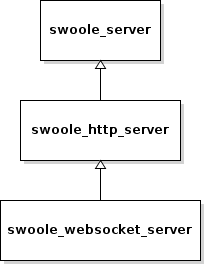
\includegraphics[scale=0.5]{swoole_server.png}
\caption{swoole\_server的继承关系}
\end{figure}

\begin{compactitem}
\item swoole\_http\_server是swoole\_server的子类,内置了Http的支持;
\item swoole\_websocket\_server是swoole\_http\_server的子类,在Http基础上内置了WebSocket的支持。
\end{compactitem}

Swoole的网络IO部分基于epoll/kqueue事件循环,因此全异步非阻塞执行,而且业务逻辑部分使用多进程同步阻塞方式来运行,从而既保证了Server能够应对高并发和大量TCP连接,又能够保证业务代码仍然可以简单地编写。





\subsection{swoole\_http\_server}




\begin{lstlisting}[language=bash]

\end{lstlisting}


\begin{lstlisting}[language=bash]

\end{lstlisting}

\begin{lstlisting}[language=bash]

\end{lstlisting}

\subsection{swoole\_websocket\_server}


\begin{lstlisting}[language=bash]

\end{lstlisting}




\begin{lstlisting}[language=bash]

\end{lstlisting}




\begin{lstlisting}[language=bash]

\end{lstlisting}




\begin{lstlisting}[language=bash]

\end{lstlisting}


\chapter{Client}

swoole\_client是TCP/UDP客户端,支持同步并发调用,也支持异步事件驱动。


\begin{lstlisting}[language=bash]

\end{lstlisting}




\begin{lstlisting}[language=bash]

\end{lstlisting}




\begin{lstlisting}[language=bash]

\end{lstlisting}


\chapter{Event}

EventLoop API\footnote{eventloop接口仅可用于socket类型的文件描述符,不能用于磁盘文件读写。},让用户可以直接操作底层的事件循环,将socket,stream,管道等Linux文件加入到事件循环中。


\section{swoole\_event}



\begin{lstlisting}[language=bash]

\end{lstlisting}




\begin{lstlisting}[language=bash]

\end{lstlisting}




\begin{lstlisting}[language=bash]

\end{lstlisting}


\chapter{Async}




\section{swoole\_async}



\begin{lstlisting}[language=bash]

\end{lstlisting}




\begin{lstlisting}[language=bash]

\end{lstlisting}




\begin{lstlisting}[language=bash]

\end{lstlisting}


\chapter{Process}


共享内存的性能虽然很好,但是存在安全问题,需要读写时加锁。

\begin{compactitem}
\item 锁的粒度过大会导致只有一个线程在运行。
\item 锁太复杂又会有死锁问题。
\end{compactitem}



\section{swoole\_process}

进程管理模块,可以方便的创建子进程,进程间通信,进程管理。

与Node.js的网络库本身没有提供多进程/多线程的实现的情况不同,swoole用户不需要自己手动管理进程的创建与回收,swoole内核根据配置文件自动完成,Node.j开发者需要自行创建进程,或者通过cluster来利用多核,否则只能使用单线程。






\begin{lstlisting}[language=bash]

\end{lstlisting}




\begin{lstlisting}[language=bash]

\end{lstlisting}




\begin{lstlisting}[language=bash]

\end{lstlisting}

\chapter{Buffer}



\section{swoole\_buffer}

强大的内存区管理工具,像C一样进行指针计算,又无需关心内存的申请和释放,而且不用担心内存越界,底层全部做好了。

\begin{lstlisting}[language=bash]

\end{lstlisting}




\begin{lstlisting}[language=bash]

\end{lstlisting}






\chapter{Table}



\section{swoole\_table}


swoole\_table是基于共享内存和自旋锁实现的超高性能内存表\footnote{swoole\_table的性能可以达到单线程每秒读写50W次。},可以彻底解决线程,进程间数据共享,加锁同步等问题。




\begin{lstlisting}[language=bash]

\end{lstlisting}





\begin{lstlisting}[language=bash]

\end{lstlisting}



















\begin{lstlisting}[language=bash]

\end{lstlisting}




\begin{lstlisting}[language=bash]

\end{lstlisting}




\begin{lstlisting}[language=bash]

\end{lstlisting}




\begin{lstlisting}[language=bash]

\end{lstlisting}




\begin{lstlisting}[language=bash]

\end{lstlisting}




\begin{lstlisting}[language=bash]

\end{lstlisting}




\begin{lstlisting}[language=bash]

\end{lstlisting}





\begin{lstlisting}[language=bash]

\end{lstlisting}




\begin{lstlisting}[language=bash]

\end{lstlisting}




\begin{lstlisting}[language=bash]

\end{lstlisting}




\begin{lstlisting}[language=bash]

\end{lstlisting}




\begin{lstlisting}[language=bash]

\end{lstlisting}




\begin{lstlisting}[language=bash]

\end{lstlisting}




\begin{lstlisting}[language=bash]

\end{lstlisting}




\begin{lstlisting}[language=bash]

\end{lstlisting}




\begin{lstlisting}[language=bash]

\end{lstlisting}




\begin{lstlisting}[language=bash]

\end{lstlisting}




\begin{lstlisting}[language=bash]

\end{lstlisting}




\begin{lstlisting}[language=bash]

\end{lstlisting}




\begin{lstlisting}[language=bash]

\end{lstlisting}




\begin{lstlisting}[language=bash]

\end{lstlisting}





\begin{lstlisting}[language=bash]

\end{lstlisting}




\begin{lstlisting}[language=bash]

\end{lstlisting}






\begin{lstlisting}[language=bash]

\end{lstlisting}




\begin{lstlisting}[language=bash]

\end{lstlisting}




\begin{lstlisting}[language=bash]

\end{lstlisting}




\begin{lstlisting}[language=bash]

\end{lstlisting}




\begin{lstlisting}[language=bash]

\end{lstlisting}




\begin{lstlisting}[language=bash]

\end{lstlisting}




\begin{lstlisting}[language=bash]

\end{lstlisting}




\begin{lstlisting}[language=bash]

\end{lstlisting}




\begin{lstlisting}[language=bash]

\end{lstlisting}




\begin{lstlisting}[language=bash]

\end{lstlisting}





\begin{lstlisting}[language=bash]

\end{lstlisting}




\begin{lstlisting}[language=bash]

\end{lstlisting}




\begin{lstlisting}[language=bash]

\end{lstlisting}




\begin{lstlisting}[language=bash]

\end{lstlisting}




\begin{lstlisting}[language=bash]

\end{lstlisting}




\begin{lstlisting}[language=bash]

\end{lstlisting}




\begin{lstlisting}[language=bash]

\end{lstlisting}




\begin{lstlisting}[language=bash]

\end{lstlisting}




\begin{lstlisting}[language=bash]

\end{lstlisting}




\begin{lstlisting}[language=bash]

\end{lstlisting}




\begin{lstlisting}[language=bash]

\end{lstlisting}




\begin{lstlisting}[language=bash]

\end{lstlisting}





\begin{lstlisting}[language=bash]

\end{lstlisting}




\begin{lstlisting}[language=bash]

\end{lstlisting}



\begin{lstlisting}[language=bash]

\end{lstlisting}




\begin{lstlisting}[language=bash]

\end{lstlisting}




\begin{lstlisting}[language=bash]

\end{lstlisting}




\begin{lstlisting}[language=bash]

\end{lstlisting}




\begin{lstlisting}[language=bash]

\end{lstlisting}




\begin{lstlisting}[language=bash]

\end{lstlisting}




\begin{lstlisting}[language=bash]

\end{lstlisting}




\begin{lstlisting}[language=bash]

\end{lstlisting}





\begin{lstlisting}[language=bash]

\end{lstlisting}




\begin{lstlisting}[language=bash]

\end{lstlisting}




\begin{lstlisting}[language=bash]

\end{lstlisting}




\begin{lstlisting}[language=bash]

\end{lstlisting}




\begin{lstlisting}[language=bash]

\end{lstlisting}




\begin{lstlisting}[language=bash]

\end{lstlisting}




\begin{lstlisting}[language=bash]

\end{lstlisting}




\begin{lstlisting}[language=bash]

\end{lstlisting}




\begin{lstlisting}[language=bash]

\end{lstlisting}




\begin{lstlisting}[language=bash]

\end{lstlisting}




\begin{lstlisting}[language=bash]

\end{lstlisting}




\begin{lstlisting}[language=bash]

\end{lstlisting}




\begin{lstlisting}[language=bash]

\end{lstlisting}




\begin{lstlisting}[language=bash]

\end{lstlisting}





\begin{lstlisting}[language=bash]

\end{lstlisting}




\begin{lstlisting}[language=bash]

\end{lstlisting}



%
\part{Server}




\chapter{Overview}

首先,软件意义上的服务器就是一个管理资源并为用户提供服务的计算机软件,通常可以分为文件服务器(能使用户在其它计算机访问文件),数据库服务器和应用程序服务器(例如TCP服务器、UDP服务器、HTTP服务器、WebSocket服务器以及异步IO和Task服务器等)。


其次,运行服务器软件的计算机一般称为网络主机(host)\footnote{服务器与主机的意义可能不同,其中主机是通过终端给用户使用的,服务器是通过网络给客户端用户使用的。},可以通过网络对外提供服务。例如,可以通过Intranet对内网提供服务,也可以通过Internet对外提供服务。

Web服务器的定义有时会引起混淆,例如可以指用于网站的计算机,也可能是指Apache或Nginx等软件,而且运行Web服务器软件的计算机可以管理网页组件和回应网页浏览器的请求。

按照服务器软件工作在客户端-服务器还是浏览器-服务器模式,可以有很多形式的服务器,例如:

\begin{compactitem}
\item 文件服务器(File Server)或网络存储设备(Network Attached Storage),例如NetWare
\item 数据库服务器(Database Server),例如Oracle,MySQL,PostgreSQL,SQL Server等
\item 邮件服务器(Mail Server),例如Sendmail、Postfix、Qmail、Microsoft Exchange、Lotus Domino等
\item 网页服务器(Web Server),例如Apache、httpd和IIS等
\item FTP服务器(FTP Server),例如Pureftpd、Proftpd、WU-ftpd、Serv-U等
\item 域名服务器(DNS Server),例如Bind9等
\item 应用程序服务器(Application Server/AP Server),例如WebLogic、JBoss和GlassFish
\item 代理服务器(Proxy Server),例如Squid cache
\item NAT服务器,例如WINS(Windows Internet Name Service)服务器
\end{compactitem}


\clearpage
\section{Echo Server} 

\begin{figure}[htbp]
\centering
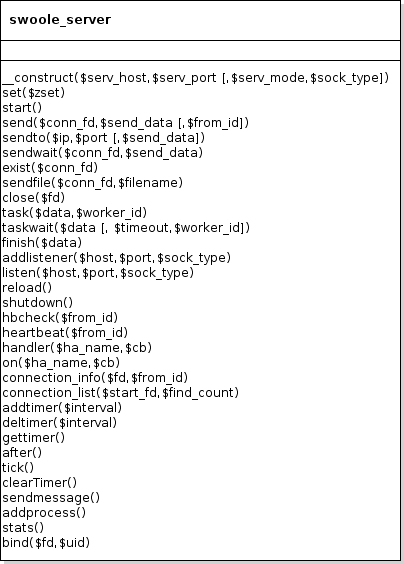
\includegraphics[scale=0.45]{class_swoole_server.png}
\caption{swoole\_server类}
\end{figure}


下面是一个基本的基于swoole的echo服务器实现,其中表示监听所有IP地址(包括 127.0.0.1、192.168.x.x 以及外网IP)。



\begin{lstlisting}[language=PHP]
<?php
// Server
class Server{
	private $serv;
	
	public function __construct(){
		$this->serv = new swoole_server("0.0.0.0",9501);
		$this->serv->set(array(
			'worker_num' => 8, // worker进程数
			'daemonize' => 0, // uint32_t, 是否守护进程化
			'max_request' => 10000, // worker进程的最大任务数
			'dispatch_mode' => 2, // 数据包分发策略,默认为2(固定模式)
			'debug_mode' => 1 // 无效参数,可以传入,不会执行
		));
		
		$this->serv->on('Start',array($this,'onStart'));
		$this->serv->on('Connect',array($this,'onConnect'));
		$this->serv->on('Receive',array($this,'onReceive'));
		$this->serv->on('Close',array($this,'onClose'));
		
		$this->serv->start();
	}
	// onStart回调在server运行前被调用
	public function onStart($serv){ 
		echo "Start\n";
	}
	// onConnect在有新客户端连接过来时被调用
	public function onConnect($serv,$fd,$from_id){ 
		$serv->send( $fd,"Hello {$fd}!" );
	}
	// onReceive函数在有数据发送到server时被调用
	public function onReceive(swoole_server $serv,$fd,$from_id,$data){
		echo "Get Message From Client {$fd}:{$data}\n";
	}
	// onClose在有客户端断开连接时被调用
	public function onClose($serv, $fd, $from_id){
		echo "Client {$fd} close connection\n";
	}
}

// 启动服务器
$server = new Server();
?>
\end{lstlisting}

创建一个swoole\_server基本分为如下三步:

\begin{compactitem}
\item 通过构造函数创建swoole\_server实例server;
\item 调用set函数设置swoole\_server实例的相关配置选项;
\item 调用on函数设置相关回调函数。
\end{compactitem}

这里,on方法的作用是注册swoole\_server的事件回调函数。

\begin{compactitem}
\item 在onStart处注册Start回调函数来启动swoole\_server实例server。
\item 在onConnect处注册Connect回调函数来让server监听新的连接。

如果有数据传入,则server可以调用send函数将处理结果发送出去。

\item 在onReceive处注册Receive回调函数来接收数据并处理。
\item 在onClose处注册Close回调函数处理客户端下线的事件。
\end{compactitem}

这里,需要注意的是启动swoole\_server实例之前,swoole\_server必须预先完成下面的操作:

\begin{compactitem}
\item 已创建了manager进程
\item 已创建了worker子进程
\item 已监听所有TCP/UDP端口
\item 已监听了定时器
\end{compactitem}

在完成上述操作后,swoole\_server的主Reactor开始接收事件,客户端可以connect到server。

onStart回调中仅允许echo、打印Log、修改进程名称,不得执行其他操作,而且onWorkerStart和onStart回调是在不同进程中并行执行的,不存在先后顺序。

在命令行中启动Echo Server的示例如下:

\begin{lstlisting}[language=PHP]
$ php server.php
Start
\end{lstlisting}

\section{Echo Client}

下面使用swoole\_client创建一个基于TCP的客户端实例,然后调用connect方法并指定同步还是模式来向指定的IP和端口发起连接请求。

\begin{compactitem}
\item 如果设置为1,则客户端使用同步阻塞模式(默认),recv和send操作都会产生网络阻塞。
\item 如果设置为0,则客户端使用异步传输模式,connect会立即返回true,但是实际上连接并未建立。
\end{compactitem}

在使用异步传输(即非阻塞socket)时,send/recv执行前必须使用swoole\_client\_select来检测是否完成了连接。

无论使用同步还是异步模式来进行数据传输,在连接成功后才可以通过recv()和send()方法来接收和发送请求。



\begin{lstlisting}[language=PHP]
<?php
// Client
class Client{
	private $client;
	
	public function __construct(){
		// 创建tcp socket
		$this->client = new swoole_client(SWOOLE_SOCK_TCP);
	}
	
	public function connect(){
		if(!$this->client->connect("127.0.0.1",9501,1)){
			echo "Error: {$fp->errMsg}[{$fp->errCode}]\n";
		}
		$message = $this->client->recv();
		echo "Get Message From Server: {$message}\n";
		
		fwrite(STDOUT,"请输入消息: ");
		$msg = trim(fgets(STDIN));
		$this->client->send($msg);
	}
}
$client = new Client();
$client->connect();
?>
\end{lstlisting}


在使用非阻塞socket时,不能在connect后使用send/recv,通过isConnected()判断也是false。只有当连接成功后,系统会自动回调onConnect,这时才可以使用send/recv。

在命令行中运行echo client的代码如下:



\begin{lstlisting}[language=PHP]
$ php client.php
Get Message From Server: Hello 1!
请输入消息:
\end{lstlisting}




\begin{lstlisting}[language=PHP]

\end{lstlisting}




\begin{lstlisting}[language=PHP]

\end{lstlisting}




\begin{lstlisting}[language=PHP]

\end{lstlisting}




\begin{lstlisting}[language=PHP]

\end{lstlisting}






\chapter{TCP}


\section{Overview}



 TCP是一种面向连接的、可靠的、基于字节流的传输层通信协议,在简化的计算机网络OSI模型中完成第四层传输层所指定的功能,用户数据报协议(UDP)则是同一层内另一个重要的传输协议。
 
 在因特网协议族(Internet protocol suite)中,TCP层是位于IP层之上,应用层之下的中间层。不同主机的应用层之间经常需要可靠的、像渠道一样的连接,但是IP层不提供这样的流机制,而是提供不可靠的包交换。

应用层向TCP层发送用于网间传输的、用8位字节表示的数据流,然后TCP把数据流分区成适当长度的报文段(通常受该计算机连接的网络的数据链路层的最大传输单元(MTU)的限制)。之后TCP把结果包传给IP层,由它来通过网络将包传送给接收端实体的TCP层。

TCP为了保证不发生丢包,就给每个包一个序号,同时序号也保证了传送到接收端实体的包的按序接收。

接收端实体对已成功收到的包发回一个相应的确认(ACK),如果发送端实体在合理的往返时延(RTT)内未收到确认,那么对应的数据包就被假设为已丢失将会被进行重传。

TCP用一个校验和函数来检验数据是否有错误,而且在发送和接收时都要计算校验和。

TCP连接包括三个状态:连接创建、数据传送和连接终止,操作系统将 TCP 连接抽象为套接字的编程接口给程序使用,因此要经历一系列的状态改变。

TCP使用了端口号(Port number)的概念来标识发送方和接收方的应用层,可能的和被正式承认的端口号有65535($2^{16}-1$)个。


对每个TCP连接的一端都有一个相关的16位的无符号端口号分配给它们,端口可以被分为三类:众所周知的、注册的和动态/私有的。

\begin{compactitem}
\item 众所周知的端口号是由因特网赋号管理局(IANA)来分配的,并且通常被用于系统一级或根进程。

众所周知的应用程序作为服务器程序来运行,并被动地侦听经常使用这些端口的连接。例如FTP、TELNET、SMTP、HTTP等。

\item 注册的端口号通常被用来作为终端用户连接服务器时短暂地使用的源端口号,但它们也可以用来标识已被第三方注册了的、被命名的服务。

\item 动态/私有的端口号在任何特定的TCP连接外不具有任何意义。

\end{compactitem}


注意,TCP并不是对所有的应用都适合,一些新的带有一些内在的脆弱性的运输层协议也被设计出来。比如,实时应用并不需要甚至无法忍受TCP的可靠传输机制。

在实时类型的应用(例如视频通话等)中,通常允许一些丢包、出错或拥塞,而不是去校正它们,因此在实时流多媒体(如因特网广播)、实时多媒体播放器和游戏、IP电话(VoIP)中可以不使用TCP。

任何不是很需要可靠性或者是想将功能减到最少的应用可以避免使用TCP,因此在很多情况下,当只需要多路复用应用服务时,用户数据报协议(UDP)可以代替TCP为应用提供服务。


\subsection{Establishment}


TCP用三路握手(three-way handshake)过程创建一个连接。在连接创建过程中,很多参数要被初始化,例如序号被初始化以保证按序传输和连接的强壮性。

一对终端同时初始化一个它们之间的连接是可能的。但通常是由一端打开一个套接字(socket)然后监听来自另一方的连接,这就是通常所指的被动打开(passive open)。服务器端被被动打开以后,用户端就能开始创建主动打开(active open)。

\begin{compactenum}
\item 客户端通过向服务器端发送一个SYN来创建一个主动打开,作为三路握手的一部分。客户端把这段连接的序号设定为随机数 A。
\item 服务器端应当为一个合法的SYN回送一个SYN/ACK。ACK 的确认码应为 A+1,SYN/ACK 包本身又有一个随机序号 B。
\item 最后,客户端再发送一个ACK。当服务端受到这个ACK的时候,就完成了三路握手,并进入了连接创建状态。此时包序号被设定为收到的确认号 A+1,而响应则为 B+1。
\end{compactenum}

\begin{figure}[htbp]
\centering
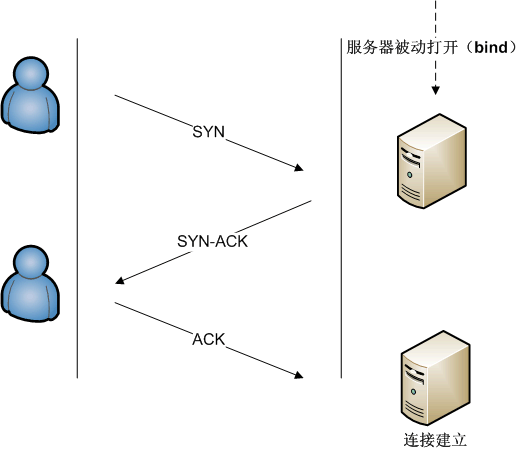
\includegraphics[scale=0.5]{Connection_TCP.png}
\caption{TCP连接的正常创建}
\end{figure}



\subsection{Transmission}

在TCP的数据传送状态,很多重要的机制保证了TCP的可靠性和强壮性,其中包括:

\begin{compactitem}
\item 使用序号,对收到的TCP报文段进行排序以及检测重复的数据;
\item 使用校验和来检测报文段的错误;
\item 使用确认和计时器来检测和纠正丢包或延时。
\end{compactitem}

在TCP的连接创建状态,两个主机的TCP层间要交换初始序号(ISN,Initial Sequence Number),而且这些序号用于标识字节流中的数据,并且还是对应用层的数据字节进行记数的整数。

通常情况下,在每个TCP报文段中都有一对序号和确认号,TCP报文发送者认为自己的字节编号为序号,而认为接收者的字节编号为确认号。

TCP报文的接收者为了确保可靠性,在接收到一定数量的连续字节流后才发送确认,其实这是对TCP的一种扩展,通常称为选择确认(Selective Acknowledgement),通过选择确认使得TCP接收者可以对乱序到达的数据块进行确认,而且每一个字节传输过后,ISN号都会递增1。


通过使用序号和确认号,TCP层可以把收到的报文段中的字节按正确的顺序交付给应用层。

序号是32位的无符号数,在它增大到$2^{32}-1$时,便会回绕到0,因此可以确保TCP中关键的一个操作——ISN的选择的强壮性和安全性。

\begin{compactenum}
\item 发送方首先发送第一个包含序列号为1(可变化)和1460字节数据的TCP报文段给接收方。接收方以一个没有数据的TCP报文段来回复(只含报头),用确认号1461来表示已完全收到并请求下一个报文段。

\item 发送方然后发送第二个包含序列号为1461和1460字节数据的TCP报文段给接收方。正常情况下,接收方以一个没有数据的TCP报文段来回复,用确认号2921(1461+1460)来表示已完全收到并请求下一个报文段。发送接收这样继续下去。

\item 然而当这些数据包都是相连的情况下,接收方没有必要每一次都回应。比如,他收到第1到5条TCP报文段,只需回应第五条就行了。在例子中第3条TCP报文段被丢失了,所以尽管他收到了第4和5条,然而他只能回应第2条。

\item 发送方在发送了第三条以后,没能收到回应,因此当定时器(timer)到期(expire)时,他重发第三条。(每次发送者发送一条TCP报文段后,都会再次启动一次时钟:RTT)。

\item 这次第三条被成功接收,接收方可以直接确认第5条,因为4,5两条已收到。

\end{compactenum}

\begin{figure}[htbp]
\centering
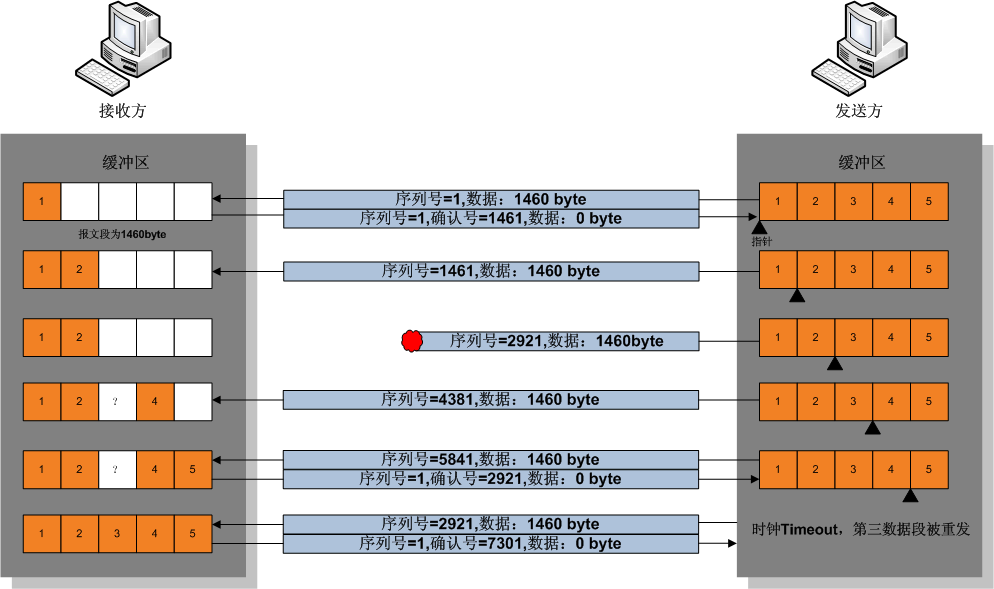
\includegraphics[scale=0.5]{Tcp_transport_example.png}
\caption{TCP数据传输}
\end{figure}

TCP的16位的校验和(checksum)的计算和检验过程如下:

发送者将TCP报文段的头部和数据部分的和计算出来,再对其求反码(一的补数),就得到了校验和,然后将结果装入报文中传输。

这里,用反码和的原因是这种方法的循环进位使校验和可以在16位、32位、64位等情况下的计算结果再叠加后相同。

接收者在收到报文后再按相同的算法计算一次校验和。这里使用的反码使得接收者不用再将校验和字段保存起来后清零,而可以直接将报文段连同校验加总。如果计算结果是全部为一,那么就表示了报文的完整性和正确性。

TCP校验和也包括了96位的伪头部,其中有源地址、目的地址、协议以及TCP的长度,从而可以避免报文被错误地路由。

按照现在的标准,TCP的校验和是一个比较脆弱的校验。出错概率高的数据链路层需要更高的能力来探测和纠正连接错误。

如果在今天重新设计TCP,很可能使用一个32位的CRC校验来纠错,而不是使用校验和。但是通过在第二层使用通常的CRC校验或更完全一点的校验可以部分地弥补这种脆弱的校验。

第二层是在TCP层和IP层之下的(比如PPP或以太网)使用了这些校验,但是这也并不意味着TCP的16位校验和是冗余的。

根据对因特网传输的观察,表明在受CRC校验保护的各跳之间,软件和硬件的错误通常也会在报文中引入错误,而端到端的TCP校验能够捕捉到很多的这种错误,这就是应用中的端到端原则。

流量控制可以避免主机分组发送得过快而使接收方来不及完全收下,因此TCP和UDP的主要不同在于:

\begin{compactitem}
\item 有序数据传输
\item 重发丢失的数据包
\item 舍弃重复的数据包
\item 无错误数据传输
\item 阻塞/流量控制
\item 面向连接(确认有创建三方交握,连接已创建才作传输)
\end{compactitem}

\subsection{Termination}

连接终止使用了四路握手过程(four-way handshake),在这个过程中每个终端的连接都能独立地被终止,因此一个典型的拆接过程需要每个终端都提供一对FIN和ACK。

\begin{figure}[htbp]
\centering
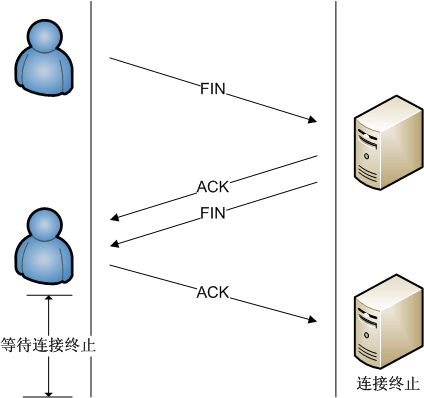
\includegraphics[scale=0.5]{Deconnection_TCP.png}
\caption{TCP连接的正常终止}
\end{figure}


\section{State Diagram}

下表为 TCP 状态码列表,以 S 指代服务器,C 指代客户端,S\&C 表示两者,S/C 表示两者之一:

\begin{figure}[htbp]
\centering
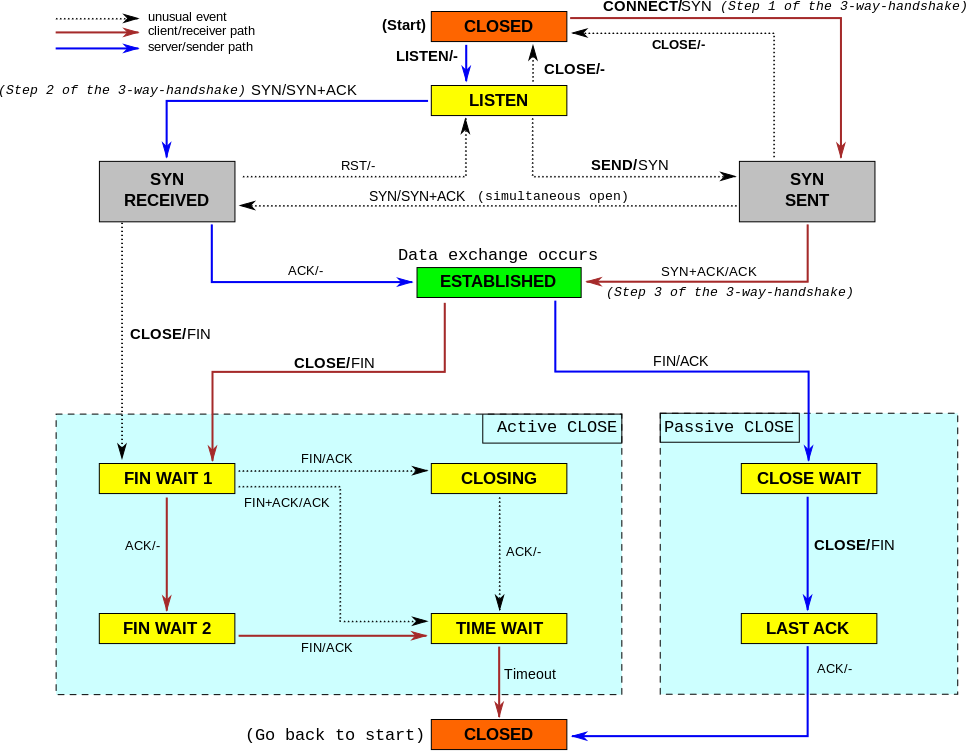
\includegraphics[scale=0.5]{Tcp_state_diagram.png}
\caption{TCP 状态码列表}
\end{figure}

\zihao{6}
\begin{longtable}{|m{70pt}|m{100pt}|m{250pt}|}
%head
\multicolumn{3}{r}{}
\tabularnewline\hline
状态码&状态&描述
\endhead
%endhead

%firsthead
\caption{TCP 状态码列表}\\
\hline
状态码&状态&描述
\endfirsthead
%endfirsthead

%foot
\multicolumn{3}{r}{}
\endfoot
%endfoot

%lastfoot
\endlastfoot
%endlastfoot

\hline
LISTEN S&侦听状态 & 等待从任意远程 TCP 端口的连接请求。\\
\hline
SYN-SENT C& 在发送连接请求后等待匹配的连接请求。&通过connect()函数向服务器发出一个同步(SYNC)信号后进入此状态。\\
\hline
SYN-RECEIVED S &  & 已经收到并发送同步(SYNC)信号之后等待确认(ACK)请求。\\
\hline
ESTABLISHED S\&C & 连接已经打开,收到的数据可以发送给用户。&数据传输步骤的正常情况。此时连接两端是平等的。\\
\hline
FIN-WAIT-1 S\&C &  & 主动关闭端调用close()函数发出FIN请求包,表示本方的数据发送全部结束,等待TCP连接另一端的确认包或FIN请求包。\\
\hline
FIN-WAIT-2 S\&C & &主动关闭端在FIN-WAIT-1状态下收到确认包,进入等待远程 TCP 的连接终止请求的半关闭状态。这时可以接收数据,但不再发送数据。\\
\hline
CLOSE-WAIT S\&C & &被动关闭端接到FIN后,就发出ACK以回应FIN请求,并进入等待本地用户的连接终止请求的半关闭状态。这时可以发送数据,但不再接收数据。\\
\hline
CLOSING S\&C & & 在发出FIN后,又收到对方发来的FIN后,进入等待对方对连接终止(FIN)的确认(ACK)的状态。\\
\hline
LAST-ACK S\&C & & 被动关闭端全部数据发送完成之后,向主动关闭端发送FIN,进入等待确认包的状态。\\
\hline
TIME-WAIT S/C &  & 主动关闭端接收到FIN后,就发送ACK包,等待足够时间\footnote{按照 RFC 793,一个连接可以在 TIME-WAIT 保证最大四分钟,即最大分段寿命(maximum segment lifetime)的2倍。}以确保被动关闭端收到了终止请求的确认包。\\
\hline
CLOSED S\&C & & 完全没有连接。\\
\hline
\end{longtable}
\zihao{5}

\clearpage

\section{TCP Server}


下面的示例创建一个TCP服务器,监听本机9501端口,当客户端Socket通过网络发送一个 hello 字符串时,服务器会回复一个 Swoole TCP Server: hello 字符串。


\begin{lstlisting}[language=PHP]
//创建swoole_server对象,在127.0.0.1监听9501端口
$serv = new swoole_server("127.0.0.1", 9501);

$serv->set(array(
    'worker_num' => 8,   //工作进程数量
    'daemonize' => 0 //是否作为守护进程
));

// 监听连接进入事件
$serv->on('connect', function ($serv, $fd){
    echo "Client:Connect.\n";
});

//监听数据发送事件
$serv->on('receive', function ($serv, $fd, $from_id, $data) {
    $serv->send($fd, 'Swoole TCP Server: '.$data);
    $serv->close($fd);
});

//监听连接关闭事件
$serv->on('close', function ($serv, $fd) {
    echo "Client: Close.\n";
});

//启动服务器
$serv->start();
\end{lstlisting}

swoole\_server是异步服务器,所以是通过监听事件的方式来编写程序的。

当对应的事件发生时底层会主动回调指定的PHP函数,例如当有新的TCP连接进入时会执行onConnect事件回调,当某个连接向服务器发送数据时会回调onReceive函数。

\begin{compactitem}
\item 服务器可以同时被成千上万个客户端连接,\texttt{\$fd}就是客户端连接的唯一标识符
\item 调用 \texttt{\$server->send()}方法向客户端连接发送数据,参数就是\texttt{\$fd}客户端标识符
\item 调用 \texttt{\$server->close()}方法可以强制关闭某个客户端连接
\item 客户端可能会主动断开连接,此时会触发onClose事件回调
\end{compactitem}

在命令行下运行server.php程序来启动Swoole TCP Server,如果启动成功后可以使用 netstat 工具看到,已经在监听9501端口,然后就可以使用telnet/netcat工具连接服务器。

\begin{lstlisting}[language=PHP]
$ php tcp_server.php 
\end{lstlisting}


\begin{compactitem}
\item 在本机使用telnet/netcat连接Swoole TCP Server:

\begin{lstlisting}[language=PHP]
$ telnet 127.0.0.1 9501
Trying 127.0.0.1...
Connected to 127.0.0.1.
Escape character is '^]'.
hello
Swoole TCP Server: hello
\end{lstlisting}

\item 在远程主机使用telnet/netcat连接Swoole TCP Server:

\begin{lstlisting}[language=PHP]
$ telnet 121.40.126.146 9501
Trying 121.40.126.146...
telnet: connect to address 121.40.126.146: Connection refused
\end{lstlisting}

\end{compactitem}




\begin{lstlisting}[language=PHP]

\end{lstlisting}




\begin{lstlisting}[language=PHP]

\end{lstlisting}




\begin{lstlisting}[language=PHP]

\end{lstlisting}







\section{TCP Client}

除了使用telnet/netcat来连接Swoole TCP Server之外,也可以自己实现TCP Client来进行连接和通信。


\begin{lstlisting}[language=PHP]
$client = new swoole_client(SWOOLE_SOCK_TCP, SWOOLE_SOCK_ASYNC);
//设置事件回调函数
$client->on("connect", function($cli) {
    $cli->send("hello world\n");
});
$client->on("receive", function($cli, $data){
    echo "Received: ".$data."\n";
});
$client->on("error", function($cli){
    echo "Connect failed\n";
});
$client->on("close", function($cli){
    echo "Connection close\n";
});
//发起网络连接
//$client->connect('127.0.0.1', 9501, 0.5);
$client->connect('121.40.126.146', 9501, 0.5);
\end{lstlisting}

\begin{compactitem}
\item SWOOLE\_SOCK\_TCP 创建tcp socket
\item SWOOLE\_SOCK\_TCP6 创建tcp ipv6 socket
\item SWOOLE\_SOCK\_UDP 创建udp socket
\item SWOOLE\_SOCK\_UDP6 创建udp ipv6 socket
\item SWOOLE\_SOCK\_SYNC 同步客户端
\item SWOOLE\_SOCK\_ASYNC 异步客户端
\end{compactitem}



在远程服务器上开启Server TCP Server:

\begin{lstlisting}[language=PHP]
$ php tcp_server.php
\end{lstlisting}

在本地计算机上执行Swoole TCP Client:

\begin{lstlisting}[language=PHP]
$ php tcp_client.php
Received: Swoole TCP Server: hello world

Connection close
\end{lstlisting}

实际上,\texttt{hello world}从远程服务器上发回,因此如果远程服务器关闭,那么就可能返回如下的错误:

\begin{lstlisting}[language=PHP]
$ php tcp_client.php
Unknown: connect to server [121.40.126.146:9501] failed. 
Error: Connection refused [111]. in Unknown on line 0

Warning: Unknown: connect to server [121.40.126.146:9501] failed. 
Error: Connection refused [111]. in Unknown on line 0

Connect failed
\end{lstlisting}

正常情况下,远程服务器上的Swoole TCP Server会产生如下的输出:


\begin{lstlisting}[language=PHP]
$ php tcp_server.php 
Client:Connect.
Client: Close.
\end{lstlisting}


\chapter{UDP}


\section{Overview}

UDP(User Datagram Protocol,用户数据报协议)是一个简单的面向数据报的传输层协议,其正式规范为 RFC 768。

在TCP/IP模型中,UDP为网络层以上和应用层以下提供了一个简单的接口。

UDP只提供数据的不可靠传递,它一旦把应用程序发给网络层的数据发送出去,就不保留数据备份,所以UDP有时候也被认为是不可靠的数据报协议,而且UDP在IP数据报的头部仅仅加入了复用和数据校验(字段)。

UDP首部字段由4个部分组成,其中两个是可选的,其中分别都是16bit的来源端口和目的端口用来标记发送和接受的应用进程。

UDP不需要应答,所以来源端口是可选的,如果来源端口不用,那么置为零。在目的端口后面是长度固定的以字节为单位的长度域,用来指定UDP数据报包括数据部分的长度,长度最小值为8byte。

首部剩下的16bit是用来对首部和数据部分一起做校验和(Checksum)的,这部分是可选的,但是在实际应用中一般都使用这一功能。

由于缺乏可靠性且属于非连接导向协定,UDP应用一般必须允许一定量的丢包、出错和复制贴上,但是有些应用(比如TFTP),如果需要则必须在应用层增加根本的可靠机制。

绝大多数UDP应用都不需要可靠机制,甚至可能因为引入可靠机制而降低性能,因此流媒体(串流技术)、即时多媒体游戏和IP电话(VoIP)一定是典型的UDP应用。如果某个应用需要很高的可靠性,那么可以用TCP来代替UDP。

由于缺乏拥塞控制(congestion control),需要基于网络的机制来减少因失控和高速UDP流量负荷而导致的拥塞崩溃效应。换句话说,因为UDP发送者不能够检测拥塞,所以像使用包队列和丢弃技术的路由器这样的网络基本设备往往就成为降低UDP过大通信量的有效工具,后来的DCCP(数据报拥塞控制协议)被设计成通过在诸如流媒体类型的高速率UDP流中,增加主机拥塞控制来减小这个潜在的问题。

基于UDP协议的关键应用在一定程度上是相似的,这些应用包括域名系统(DNS)、简单网络管理协议(SNMP)、动态主机配置协议(DHCP)、路由信息协议(RIP)和某些影音串流服务等等。


\section{UDP Server}

Swoole支持CPU Affinity设置,守护进程化,并且混合UDP/TCP多端口监听,多定时器等。

\begin{lstlisting}[language=PHP]
//创建Server对象,监听 127.0.0.1:9502端口,类型为SWOOLE_SOCK_UDP
$serv = new swoole_server("127.0.0.1", 9502, SWOOLE_PROCESS, SWOOLE_SOCK_UDP); 
$server->set(['worker_num' => 1]);

//监听数据发送事件
$server->on('Packet', function (swoole_server $serv, $data, $addr)
{
    $serv->sendto($addr['address'], $addr['port'], "Swoole UDP Server: $data" );
    var_dump( $addr, strlen($data));
});

//启动服务器
$serv->start(); 
\end{lstlisting}

UDP服务器与TCP服务器不同,UDP没有连接的概念,因此启动Server后,客户端无需Connect,直接可以向Server监听的9502端口发送数据包,服务器端对应的事件为onPacket。

\begin{compactitem}
\item \texttt{\$clientInfo}是客户端的相关信息,是一个数组,有客户端的IP和端口等内容
\item 调用 \texttt{\$server->send}方法向客户端发送数据
\end{compactitem}


在启动Swoole UDP Server后就可以使用netcat来尝试连接,或者自己实现UDP Client来连接。

\begin{lstlisting}[language=PHP]
$ php udp_server.php
$ netcat -u 127.0.0.1 9502
\end{lstlisting}




\begin{lstlisting}[language=PHP]

\end{lstlisting}






\begin{lstlisting}[language=PHP]

\end{lstlisting}


\section{UDP Client}


\begin{lstlisting}[language=PHP]
 <?php
$client = new swoole_client(SWOOLE_SOCK_UDP,SWOOLE_SOCK_SYNC);
$client->connect('127.0.0.1',9502);
$client->send("UDP Connection from bz");
echo $client->recv();
?>
\end{lstlisting}

\begin{compactitem}
\item 如果从本地执行udp\_server.php,那么首先会看到UDP服务器在等待接收客户端数据传入。
\item 如果从本地执行udp\_client.php,那么UDP客户端首先向UDP服务器发送数据,然后接收UDP服务器响应。
\item 在接收到UDP客户端发送的数据并回送响应后,UDP服务器会输出关于UDP客户端连接的数据。
\end{compactitem}


\begin{lstlisting}[language=PHP]
$ php udp_server.php

$ php udp_client.php
Swoole UDP Server: UDP Connection from bz
$ php udp_server.php
array(3) {
  ["server_socket"]=>
  int(3)
  ["address"]=>
  string(9) "127.0.0.1"
  ["port"]=>
  int(42617)
}
int(22)
\end{lstlisting}




\begin{lstlisting}[language=PHP]

\end{lstlisting}




\begin{lstlisting}[language=PHP]

\end{lstlisting}




\begin{lstlisting}[language=PHP]

\end{lstlisting}




\begin{lstlisting}[language=PHP]

\end{lstlisting}





\chapter{HTTP}


\section{Overview}

最初,设计HTTP(HyperText Transfer Protocol,超文本转移协议)的目的是为了提供一种发布和接收HTML页面的方法,并且统一使用URI(Uniform Resource Identifiers)来标识HTTP或者HTTPS协议请求的资源。


现在,HTTP已经演化为一个客户端终端(用户)和服务器端(网站)请求和应答的标准(TCP)。

\begin{compactitem}
\item 通过使用Web浏览器、网络爬虫或者其它的工具,客户端发起一个HTTP请求到服务器上指定端口(默认端口为80),我们称这个客户端为用户代理程序(user agent)。
\item 应答的HTTP服务器上存储着一些资源,比如HTML文件和图像,我们称这个应答服务器为源服务器(origin server)。
\item 在用户代理和源服务器中间可能存在多个“中间层”,比如代理服务器、网关或者隧道(tunnel)。
\end{compactitem}

尽管TCP/IP协议是互联网上最流行的应用,但是HTTP协议中并没有规定必须使用它或它支持的层,事实上HTTP可以在任何互联网协议上,或其他网络上实现。

HTTP假定其下层协议提供可靠的传输,因此任何能够提供这种保证的协议都可以被其使用,因此构建在TCP/IP协议族之上的HTTP协议使用TCP作为其传输层。

通常情况下,由HTTP客户端发起一个请求,并创建一个到服务器指定端口(默认是80端口)的TCP连接。

HTTP服务器会以守护进程形式运行,并且在对应的端口监听客户端的请求,这样一旦收到请求,服务器就会向客户端返回一个状态(比如\texttt{"HTTP/1.1 200 OK"})以及返回的内容,例如请求的文件、错误消息或者其它信息。


超文本传输协议已经演化出了很多版本,它们中的大部分都是向下兼容的。

\begin{compactitem}
\item 客户端在请求的开始告诉服务器它采用的协议版本号。

\item 服务器在响应中采用相同或者更早的协议版本。
\end{compactitem}


在HTTP 0.9和1.0\footnote{HTTP 1.0是第一个在通讯中指定版本号的HTTP协议版本,至今仍被广泛采用(特别是在代理服务器中)。}使用非持续连接,非持续连接下的每个tcp只连接一个Web对象,连接在每个请求-回应对后都会关闭,一个连接可被多个请求重复利用的保持连接机制被引入。

这种连接持续化显著地减少了请求延迟,因为客户不用在首次请求后再次进行TCP交互确认创建连接,现在在HTTP 1.1已经默认使用持续连接,不必为每个web对象创建一个新的连接,一个连接可以传送多个对象。 



HTTP/1.1相较于HTTP/1.0协议的区别主要体现在:

\begin{compactitem}
\item 缓存处理
\item 带宽优化及网络连接的使用
\item 错误通知的管理
\item 消息在网络中的发送
\item 互联网地址的维护
\item 安全性及完整性
\end{compactitem}

HTTP1.1还进行了带宽优化,例如1.1引入了分块传输编码来允许流化传输持续连接上发送的内容,取代原先的buffer式传输。

HTTP 1.1能很好地配合代理服务器工作,而且还支持以渠道方式在同时发送多个请求,以便降低线路负载,提高传输速度,HTTP渠道允许客户在上一个回应被收到前发送多重请求从而进一步减少了延迟时间。

另一项协议的改进是byte serving(字节服务),允许服务器根据客户的请求仅仅传输资源的一部分。

\begin{compactitem}
\item 在HTTP1.0,单一TCP连接内仅执行一个“客户端发送请求—服务器发送应答”周期,之后释放TCP连接。
\item 在HTTP1.1优化支持持续活跃连接:客户端连续多次发送请求、接收应答;批量多请求时,同一TCP连接在活跃(Keep-Live)间期内复用,避免重复TCP初始握手活动,减少网络负荷和响应周期。
\end{compactitem}

此外,支持应答到达前继续发送请求(通常是两个),称为“流线化”(stream)。



\subsection{Request Message}

HTTP客户端发出的请求信息包括请求行、(请求)头、空行和其他消息体。

\begin{compactitem}
\item 请求行,例如\texttt{GET /images/logo.gif HTTP/1.1}表示从/images目录下请求logo.gif这个文件。
\item (请求)头,例如\texttt{Accept-Language: en}
\item 空行
\item 其他消息体
\end{compactitem}

请求行和标题必须以<CR><LF>作为结尾,而且空行内必须只有<CR><LF>而无其他空格。

在HTTP/1.1协议中,所有的请求头,除Host外都是可选的。




\subsection{Request Method}


HTTP/1.1协议中共定义了8种方法(也叫“动作”)来以不同方式操作指定的资源。

\zihao{6}
\begin{longtable}{|m{50pt}|m{150pt}|m{250pt}|}
%head
\multicolumn{3}{r}{}
\tabularnewline\hline
方法&说明&应用
\endhead
%endhead

%firsthead
\caption{HTTP 1.1请求方法}\\
\hline
方法&说明&应用
\endfirsthead
%endfirsthead

%foot
\multicolumn{3}{r}{}
\endfoot
%endfoot

%lastfoot
\endlastfoot
%endlastfoot

\hline
OPTIONS& OPTION方法可使服务器传回该资源所支持的所有HTTP请求方法。&用'*'来代替资源名称向Web服务器发送OPTIONS请求,可以测试服务器功能是否正常运作。\\
\hline
HEAD&与GET方法一样,都是向服务器发出指定资源的请求。只不过服务器将不传回资源的本文部分。&HEAD方法的好处在于,使用这个方法可以在不必传输全部内容的情况下,就可以获取其中“关于该资源的信息”(元信息或称元数据)。\\
\hline
GET&向指定的资源发出“显示”请求。&使用GET方法应该只用在读取数据,而不应当被用于产生“副作用”的操作中(例如Web Application),还有一个原因是GET可能会被网络蜘蛛等随意访问。\\
\hline
POST&向指定资源提交数据,请求服务器进行处理(例如提交表单或者上传文件)。&数据被包含在请求本文中。这个请求可能会创建新的资源或修改现有资源,或二者皆有。\\
\hline
PUT&向指定资源位置上传其最新内容。&\\
\hline
DELETE&请求服务器删除Request-URI所标识的资源。&\\
\hline
TRACE&回显服务器收到的请求,主要用于测试或诊断。&\\
\hline
CONNECT&HTTP/1.1协议中预留给能够将连接改为渠道方式的代理服务器。&通常用于SSL加密服务器的链接(经由非加密的HTTP代理服务器)。\\
\hline
PATCH(可选)&用于将局部修改应用到资源。&由 RFC 5789 指定的方法\\
\hline
\end{longtable}
\zihao{5}


方法名称是区分大小写的,而且HTTP服务器至少应该实现GET和HEAD方法,其他方法都是可选的。

下面是一个HTTP客户端与服务器之间会话的例子,运行于www.google.com,端口80。

\begin{compactitem}
\item 客户端请求

\begin{lstlisting}[language=PHP]
GET / HTTP/1.1
Host: www.google.com
\end{lstlisting}

客户端请求的末尾有一个空行。第一行指定方法、资源路径、协议版本;第二行是在1.1版里必带的一个header作用指定主机

\item 服务器应答

\begin{lstlisting}[language=PHP]
HTTP/1.1 200 OK
Content-Length: 3059
Server: GWS/2.0
Date: Sat, 11 Jan 2003 02:44:04 GMT
Content-Type: text/html
Cache-control: private
Set-Cookie: PREF=ID=73d4aef52e57bae9:TM=1042253044:LM=1042253044:S=SMCc_HRPCQiqy
X9j; expires=Sun, 17-Jan-2038 19:14:07 GMT; path=/; domain=.google.com
Connection: keep-alive
\end{lstlisting}

服务器应答头的末尾紧跟着一个空行,并且由HTML格式的文本组成了Google的主页。

\end{compactitem}







当某个请求所针对的资源不支持对应的请求方法的时候,服务器应当返回状态码405(Method Not Allowed),当服务器不认识或者不支持对应的请求方法的时候,应当返回状态码501(Not Implemented)。


当然,所有的方法支持的实现都应当符合各自的语义定义。此外,除了上述方法,特定的HTTP服务器还能够扩展自定义的方法(例如PATCH)。



\subsection{Safe Method}


对于GET和HEAD方法而言,除了进行获取资源信息外,这些请求不应当再有其他意义。也就是说,这些方法应当被认为是“安全的”。 

客户端可能会使用其他“非安全”方法(例如POST,PUT及DELETE),应该以特殊的方式(通常是按钮而不是超链接)告知客户可能的后果(例如一个按钮控制的资金交易),或请求的操作可能是不安全的(例如某个文件将被上传或删除)。

不过,不能想当然地认为服务器在处理某个GET请求时不会产生任何副作用。

事实上,很多动态资源会把这作为其特性,这里重要的区别在于用户并没有请求这一副作用,因此不应由用户为这些副作用承担责任。




\subsection{Side Reaction}


假如在不考虑诸如错误或者过期等问题的情况下,若干次请求的副作用与单次请求相同或者根本没有副作用,那么这些请求方法就能够被视作“幂等”的。GET,HEAD,PUT和DELETE方法都有这样的幂等属性,同样由于根据协议,OPTIONS,TRACE都不应有副作用,因此也理所当然也是幂等的。

假如某个由若干个请求做成的请求序列产生的结果在重复执行这个请求序列或者其中任何一个或多个请求后仍没有发生变化,则这个请求序列便是“幂等”的。但是,可能出现若干个请求做成的请求序列是“非幂等”的,即使这个请求序列中所有执行的请求方法都是幂等的。例如,这个请求序列的结果依赖于某个会在下次执行这个序列的过程中被修改的变量。


\subsection{Status Code}


所有HTTP响应的第一行都是状态行,依次是当前HTTP版本号,3位数字组成的状态代码,以及描述状态的短语,彼此由空格分隔。

状态代码的第一个数字代表当前响应的类型:

\begin{compactitem}
\item 1xx消息——请求已被服务器接收,继续处理
\item 2xx成功——请求已成功被服务器接收、理解、并接受
\item 3xx重定向——需要后续操作才能完成这一请求
\item 4xx请求错误——请求含有词法错误或者无法被执行
\item 5xx服务器错误——服务器在处理某个正确请求时发生错误
\end{compactitem}

虽然 RFC 2616 中已经推荐了描述状态的短语,例如\texttt{"200 OK"}和\texttt{"404 Not Found"}等,但是Web开发者仍然能够自行决定采用何种短语,用以显示本地化的状态描述或者自定义信息。






\subsection{HTTPS}

目前有两种方法来创建安全超文本协议连接,分别是HTTPS URI方案和HTTP 1.1请求头(由 RFC 2817 引入)。

由于浏览器对后者的几乎没有任何支持,因此HTTPS URI方案仍是创建安全超文本协议连接的主要手段,安全超文本连接协议使用https://代替http://。




\begin{lstlisting}[language=PHP]

\end{lstlisting}




\begin{lstlisting}[language=PHP]

\end{lstlisting}


\section{HTTP Server}


\begin{lstlisting}[language=PHP]
$serv = new swoole_http_server("127.0.0.1", 9502);

$serv->on('Request', function($request, $response) {
    var_dump($request->get);
    var_dump($request->post);
    var_dump($request->cookie);
    var_dump($request->files);
    var_dump($request->header);
    var_dump($request->server);

    $response->cookie("User", "Swoole");
    $response->header("X-Server", "Swoole");
    $response->end("<h1>Hello Swoole!</h1>");
});

$serv->start();
\end{lstlisting}


\section{HTTPS Server}





\chapter{WebSocket Server}


\begin{lstlisting}[language=PHP]
<?php
/**
 * 创建WebSocket Server
 */
$serv = new swoole_websocket_server("127.0.0.1", 9502);

/**
 * 注册Server的事件回调函数open
 */
$serv->on('Open', function($server, $req) {
    echo "connection open: ".$req->fd;
});
/**
 * 注册Server的事件回调函数message
 */
$serv->on('Message', function($server, $frame) {
    echo "message: ".$frame->data;
    $server->push($frame->fd, json_encode(["hello", "world"]));
});
/**
 * 注册Server的事件回调函数close
 */
$serv->on('Close', function($server, $fd) {
    echo "connection close: ".$fd;
});

/**
 * 启动WebSocket Server
 */
$serv->start();
?>
\end{lstlisting}

\begin{figure}[htbp]
\centering
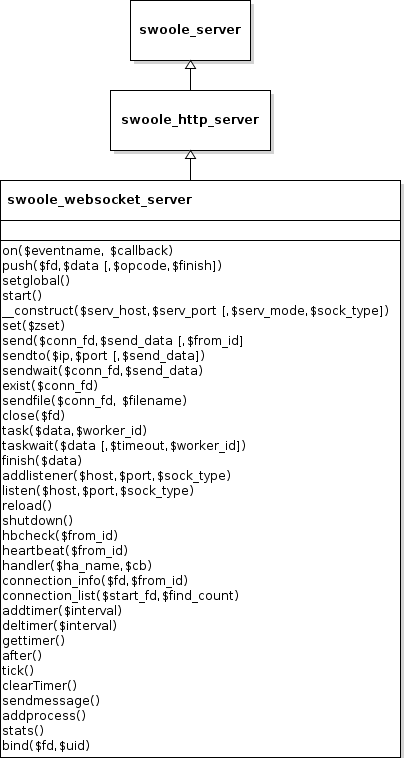
\includegraphics[scale=0.45]{class_swoole_websocket_server.png}
\caption{swoole\_websocket\_server类}
\end{figure}

\begin{compactitem}
\item \texttt{\$fd}:TCP连接的文件描述符(file description),在swoole\_server中是客户端的唯一标识符。
\item \texttt{\$from\_id}:来自于哪个reactor线程。
\item \texttt{\$conn\_fd}:网络字节序(long类型字段,IPv4的第4字节最小为1)。
\end{compactitem}


\begin{lstlisting}[language=PHP]

\end{lstlisting}


\section{WS Server}


\begin{lstlisting}[language=PHP]
<?php
/**
 * 创建WebSocket Server
 */
$wsserver = new swoole_websocket_server("127.0.0.1", 9502);

/**
 * 注册Server的事件回调函数open
 */
$wsserver->on('Open', function($server, $req) {
    echo "connection open: ".$req->fd;
});

/**
 * 注册Server的事件回调函数message
 */
$wsserver->on('Message', function($server, $frame) {
    echo "message: ".$frame->data;
    $server->push($frame->fd, json_encode(["hello", "world"]));
});

/**
 * 注册Server的事件回调函数close
 */
$wsserver->on('Close', function($server, $fd) {
    echo "connection close: ".$fd;
});

/**
 * 启动WebSocket Server
 */
$wsserver->start();
?>
\end{lstlisting}




\begin{lstlisting}[language=PHP]

\end{lstlisting}



\begin{lstlisting}[language=PHP]

\end{lstlisting}


\begin{lstlisting}[language=PHP]

\end{lstlisting}






\begin{lstlisting}[language=PHP]

\end{lstlisting}



\begin{lstlisting}[language=PHP]

\end{lstlisting}



\begin{lstlisting}[language=PHP]

\end{lstlisting}





\section{WSS Server}


\begin{lstlisting}[language=PHP]

\end{lstlisting}





\begin{lstlisting}[language=PHP]
<?php
$wssserver = new swoole_websocket_server("0.0.0.0",9527,SWOOLE_PROCESS,);
?>
\end{lstlisting}




\begin{lstlisting}[language=PHP]

\end{lstlisting}




\begin{lstlisting}[language=PHP]

\end{lstlisting}


\chapter{WebSocket Client}

\begin{lstlisting}[language=PHP]

\end{lstlisting}




\begin{lstlisting}[language=PHP]

\end{lstlisting}




\begin{lstlisting}[language=PHP]

\end{lstlisting}




\begin{lstlisting}[language=PHP]

\end{lstlisting}


\chapter{Async-IO}

\begin{lstlisting}[language=PHP]
$fp = stream_socket_client("tcp://127.0.0.1:80", $code, $msg, 3);
$http_request = "GET /index.html HTTP/1.1\r\n\r\n";
fwrite($fp, $http_request);
swoole_event_add($fp, function($fp){
    echo fread($fp, 8192);
    swoole_event_del($fp);
    fclose($fp);
});
swoole_timer_after(2000, function() {
    echo "2000ms timeout\n";
});
swoole_timer_tick(1000, function() {
    echo "1000ms interval\n";
});
\end{lstlisting}




\begin{lstlisting}[language=PHP]

\end{lstlisting}




\begin{lstlisting}[language=PHP]

\end{lstlisting}


\chapter{Task}


\begin{lstlisting}[language=PHP]
$serv = new swoole_server("127.0.0.1", 9502);
$serv->set(array('task_worker_num' => 4));
$serv->on('Receive', function($serv, $fd, $from_id, $data) {
    $task_id = $serv->task("Async");
    echo "Dispath AsyncTask: id=$task_id\n";
});
$serv->on('Task', function ($serv, $task_id, $from_id, $data) {
    echo "New AsyncTask[id=$task_id]".PHP_EOL;
    $serv->finish("$data -> OK");
});
$serv->on('Finish', function ($serv, $task_id, $data) {
    echo "AsyncTask[$task_id] Finish: $data".PHP_EOL;
});
$serv->start();
\end{lstlisting}




\begin{lstlisting}[language=PHP]

\end{lstlisting}






\begin{lstlisting}[language=PHP]

\end{lstlisting}




\begin{lstlisting}[language=PHP]

\end{lstlisting}




\begin{lstlisting}[language=PHP]

\end{lstlisting}




\begin{lstlisting}[language=PHP]

\end{lstlisting}




\begin{lstlisting}[language=PHP]

\end{lstlisting}




\begin{lstlisting}[language=PHP]

\end{lstlisting}




\begin{lstlisting}[language=PHP]

\end{lstlisting}




\begin{lstlisting}[language=PHP]

\end{lstlisting}




\begin{lstlisting}[language=PHP]

\end{lstlisting}




\begin{lstlisting}[language=PHP]

\end{lstlisting}





\begin{lstlisting}[language=PHP]

\end{lstlisting}




\begin{lstlisting}[language=PHP]

\end{lstlisting}




\begin{lstlisting}[language=PHP]

\end{lstlisting}




\begin{lstlisting}[language=PHP]

\end{lstlisting}




\begin{lstlisting}[language=PHP]

\end{lstlisting}




\begin{lstlisting}[language=PHP]

\end{lstlisting}




\begin{lstlisting}[language=PHP]

\end{lstlisting}




\begin{lstlisting}[language=PHP]

\end{lstlisting}




\begin{lstlisting}[language=PHP]

\end{lstlisting}




\begin{lstlisting}[language=PHP]

\end{lstlisting}




\begin{lstlisting}[language=PHP]

\end{lstlisting}




\begin{lstlisting}[language=PHP]

\end{lstlisting}





\begin{lstlisting}[language=PHP]

\end{lstlisting}




\begin{lstlisting}[language=PHP]

\end{lstlisting}



\begin{lstlisting}[language=PHP]

\end{lstlisting}




\begin{lstlisting}[language=PHP]

\end{lstlisting}




\begin{lstlisting}[language=PHP]

\end{lstlisting}




\begin{lstlisting}[language=PHP]

\end{lstlisting}




\begin{lstlisting}[language=PHP]

\end{lstlisting}




\begin{lstlisting}[language=PHP]

\end{lstlisting}




\begin{lstlisting}[language=PHP]

\end{lstlisting}




\begin{lstlisting}[language=PHP]

\end{lstlisting}





\begin{lstlisting}[language=PHP]

\end{lstlisting}




\begin{lstlisting}[language=PHP]

\end{lstlisting}




\begin{lstlisting}[language=PHP]

\end{lstlisting}




\begin{lstlisting}[language=PHP]

\end{lstlisting}




\begin{lstlisting}[language=PHP]

\end{lstlisting}




\begin{lstlisting}[language=PHP]

\end{lstlisting}




\begin{lstlisting}[language=PHP]

\end{lstlisting}




\begin{lstlisting}[language=PHP]

\end{lstlisting}




\begin{lstlisting}[language=PHP]

\end{lstlisting}




\begin{lstlisting}[language=PHP]

\end{lstlisting}




\begin{lstlisting}[language=PHP]

\end{lstlisting}




\begin{lstlisting}[language=PHP]

\end{lstlisting}




\begin{lstlisting}[language=PHP]

\end{lstlisting}




\begin{lstlisting}[language=PHP]

\end{lstlisting}





\begin{lstlisting}[language=PHP]

\end{lstlisting}




\begin{lstlisting}[language=PHP]

\end{lstlisting}







\begin{lstlisting}[language=PHP]

\end{lstlisting}





\begin{lstlisting}[language=PHP]

\end{lstlisting}



















\begin{lstlisting}[language=PHP]

\end{lstlisting}




\begin{lstlisting}[language=PHP]

\end{lstlisting}




\begin{lstlisting}[language=PHP]

\end{lstlisting}




\begin{lstlisting}[language=PHP]

\end{lstlisting}




\begin{lstlisting}[language=PHP]

\end{lstlisting}




\begin{lstlisting}[language=PHP]

\end{lstlisting}




\begin{lstlisting}[language=PHP]

\end{lstlisting}





\begin{lstlisting}[language=PHP]

\end{lstlisting}




\begin{lstlisting}[language=PHP]

\end{lstlisting}




\begin{lstlisting}[language=PHP]

\end{lstlisting}




\begin{lstlisting}[language=PHP]

\end{lstlisting}




\begin{lstlisting}[language=PHP]

\end{lstlisting}




\begin{lstlisting}[language=PHP]

\end{lstlisting}




\begin{lstlisting}[language=PHP]

\end{lstlisting}




\begin{lstlisting}[language=PHP]

\end{lstlisting}




\begin{lstlisting}[language=PHP]

\end{lstlisting}




\begin{lstlisting}[language=PHP]

\end{lstlisting}




\begin{lstlisting}[language=PHP]

\end{lstlisting}




\begin{lstlisting}[language=PHP]

\end{lstlisting}




\begin{lstlisting}[language=PHP]

\end{lstlisting}




\begin{lstlisting}[language=PHP]

\end{lstlisting}





\begin{lstlisting}[language=PHP]

\end{lstlisting}




\begin{lstlisting}[language=PHP]

\end{lstlisting}






\begin{lstlisting}[language=PHP]

\end{lstlisting}




\begin{lstlisting}[language=PHP]

\end{lstlisting}




\begin{lstlisting}[language=PHP]

\end{lstlisting}




\begin{lstlisting}[language=PHP]

\end{lstlisting}




\begin{lstlisting}[language=PHP]

\end{lstlisting}




\begin{lstlisting}[language=PHP]

\end{lstlisting}




\begin{lstlisting}[language=PHP]

\end{lstlisting}




\begin{lstlisting}[language=PHP]

\end{lstlisting}




\begin{lstlisting}[language=PHP]

\end{lstlisting}




\begin{lstlisting}[language=PHP]

\end{lstlisting}





\begin{lstlisting}[language=PHP]

\end{lstlisting}




\begin{lstlisting}[language=PHP]

\end{lstlisting}




\begin{lstlisting}[language=PHP]

\end{lstlisting}




\begin{lstlisting}[language=PHP]

\end{lstlisting}




\begin{lstlisting}[language=PHP]

\end{lstlisting}




\begin{lstlisting}[language=PHP]

\end{lstlisting}




\begin{lstlisting}[language=PHP]

\end{lstlisting}




\begin{lstlisting}[language=PHP]

\end{lstlisting}




\begin{lstlisting}[language=PHP]

\end{lstlisting}




\begin{lstlisting}[language=PHP]

\end{lstlisting}




\begin{lstlisting}[language=PHP]

\end{lstlisting}




\begin{lstlisting}[language=PHP]

\end{lstlisting}





\begin{lstlisting}[language=PHP]

\end{lstlisting}




\begin{lstlisting}[language=PHP]

\end{lstlisting}



\begin{lstlisting}[language=PHP]

\end{lstlisting}




\begin{lstlisting}[language=PHP]

\end{lstlisting}




\begin{lstlisting}[language=PHP]

\end{lstlisting}




\begin{lstlisting}[language=PHP]

\end{lstlisting}




\begin{lstlisting}[language=PHP]

\end{lstlisting}




\begin{lstlisting}[language=PHP]

\end{lstlisting}




\begin{lstlisting}[language=PHP]

\end{lstlisting}




\begin{lstlisting}[language=PHP]

\end{lstlisting}





\begin{lstlisting}[language=PHP]

\end{lstlisting}




\begin{lstlisting}[language=PHP]

\end{lstlisting}




\begin{lstlisting}[language=PHP]

\end{lstlisting}




\begin{lstlisting}[language=PHP]

\end{lstlisting}




\begin{lstlisting}[language=PHP]

\end{lstlisting}




\begin{lstlisting}[language=PHP]

\end{lstlisting}




\begin{lstlisting}[language=PHP]

\end{lstlisting}




\begin{lstlisting}[language=PHP]

\end{lstlisting}




\begin{lstlisting}[language=PHP]

\end{lstlisting}




\begin{lstlisting}[language=PHP]

\end{lstlisting}




\begin{lstlisting}[language=PHP]

\end{lstlisting}




\begin{lstlisting}[language=PHP]

\end{lstlisting}




\begin{lstlisting}[language=PHP]

\end{lstlisting}




\begin{lstlisting}[language=PHP]

\end{lstlisting}





\begin{lstlisting}[language=PHP]

\end{lstlisting}




\begin{lstlisting}[language=PHP]

\end{lstlisting}







\begin{lstlisting}[language=PHP]

\end{lstlisting}





\begin{lstlisting}[language=PHP]

\end{lstlisting}



















\begin{lstlisting}[language=PHP]

\end{lstlisting}




\begin{lstlisting}[language=PHP]

\end{lstlisting}




\begin{lstlisting}[language=PHP]

\end{lstlisting}




\begin{lstlisting}[language=PHP]

\end{lstlisting}




\begin{lstlisting}[language=PHP]

\end{lstlisting}




\begin{lstlisting}[language=PHP]

\end{lstlisting}




\begin{lstlisting}[language=PHP]

\end{lstlisting}





\begin{lstlisting}[language=PHP]

\end{lstlisting}




\begin{lstlisting}[language=PHP]

\end{lstlisting}




\begin{lstlisting}[language=PHP]

\end{lstlisting}




\begin{lstlisting}[language=PHP]

\end{lstlisting}




\begin{lstlisting}[language=PHP]

\end{lstlisting}




\begin{lstlisting}[language=PHP]

\end{lstlisting}




\begin{lstlisting}[language=PHP]

\end{lstlisting}




\begin{lstlisting}[language=PHP]

\end{lstlisting}




\begin{lstlisting}[language=PHP]

\end{lstlisting}




\begin{lstlisting}[language=PHP]

\end{lstlisting}




\begin{lstlisting}[language=PHP]

\end{lstlisting}




\begin{lstlisting}[language=PHP]

\end{lstlisting}




\begin{lstlisting}[language=PHP]

\end{lstlisting}




\begin{lstlisting}[language=PHP]

\end{lstlisting}





\begin{lstlisting}[language=PHP]

\end{lstlisting}




\begin{lstlisting}[language=PHP]

\end{lstlisting}






\begin{lstlisting}[language=PHP]

\end{lstlisting}




\begin{lstlisting}[language=PHP]

\end{lstlisting}




\begin{lstlisting}[language=PHP]

\end{lstlisting}




\begin{lstlisting}[language=PHP]

\end{lstlisting}




\begin{lstlisting}[language=PHP]

\end{lstlisting}




\begin{lstlisting}[language=PHP]

\end{lstlisting}




\begin{lstlisting}[language=PHP]

\end{lstlisting}




\begin{lstlisting}[language=PHP]

\end{lstlisting}




\begin{lstlisting}[language=PHP]

\end{lstlisting}




\begin{lstlisting}[language=PHP]

\end{lstlisting}





\begin{lstlisting}[language=PHP]

\end{lstlisting}




\begin{lstlisting}[language=PHP]

\end{lstlisting}




\begin{lstlisting}[language=PHP]

\end{lstlisting}




\begin{lstlisting}[language=PHP]

\end{lstlisting}




\begin{lstlisting}[language=PHP]

\end{lstlisting}




\begin{lstlisting}[language=PHP]

\end{lstlisting}




\begin{lstlisting}[language=PHP]

\end{lstlisting}




\begin{lstlisting}[language=PHP]

\end{lstlisting}




\begin{lstlisting}[language=PHP]

\end{lstlisting}




\begin{lstlisting}[language=PHP]

\end{lstlisting}




\begin{lstlisting}[language=PHP]

\end{lstlisting}




\begin{lstlisting}[language=PHP]

\end{lstlisting}





\begin{lstlisting}[language=PHP]

\end{lstlisting}




\begin{lstlisting}[language=PHP]

\end{lstlisting}



\begin{lstlisting}[language=PHP]

\end{lstlisting}




\begin{lstlisting}[language=PHP]

\end{lstlisting}




\begin{lstlisting}[language=PHP]

\end{lstlisting}




\begin{lstlisting}[language=PHP]

\end{lstlisting}




\begin{lstlisting}[language=PHP]

\end{lstlisting}




\begin{lstlisting}[language=PHP]

\end{lstlisting}




\begin{lstlisting}[language=PHP]

\end{lstlisting}




\begin{lstlisting}[language=PHP]

\end{lstlisting}





\begin{lstlisting}[language=PHP]

\end{lstlisting}




\begin{lstlisting}[language=PHP]

\end{lstlisting}




\begin{lstlisting}[language=PHP]

\end{lstlisting}




\begin{lstlisting}[language=PHP]

\end{lstlisting}




\begin{lstlisting}[language=PHP]

\end{lstlisting}




\begin{lstlisting}[language=PHP]

\end{lstlisting}




\begin{lstlisting}[language=PHP]

\end{lstlisting}




\begin{lstlisting}[language=PHP]

\end{lstlisting}




\begin{lstlisting}[language=PHP]

\end{lstlisting}




\begin{lstlisting}[language=PHP]

\end{lstlisting}




\begin{lstlisting}[language=PHP]

\end{lstlisting}




\begin{lstlisting}[language=PHP]

\end{lstlisting}




\begin{lstlisting}[language=PHP]

\end{lstlisting}




\begin{lstlisting}[language=PHP]

\end{lstlisting}





\begin{lstlisting}[language=PHP]

\end{lstlisting}




\begin{lstlisting}[language=PHP]

\end{lstlisting}








\begin{lstlisting}[language=PHP]

\end{lstlisting}





\begin{lstlisting}[language=PHP]

\end{lstlisting}



















\begin{lstlisting}[language=PHP]

\end{lstlisting}




\begin{lstlisting}[language=PHP]

\end{lstlisting}




\begin{lstlisting}[language=PHP]

\end{lstlisting}




\begin{lstlisting}[language=PHP]

\end{lstlisting}




\begin{lstlisting}[language=PHP]

\end{lstlisting}




\begin{lstlisting}[language=PHP]

\end{lstlisting}




\begin{lstlisting}[language=PHP]

\end{lstlisting}





\begin{lstlisting}[language=PHP]

\end{lstlisting}




\begin{lstlisting}[language=PHP]

\end{lstlisting}




\begin{lstlisting}[language=PHP]

\end{lstlisting}




\begin{lstlisting}[language=PHP]

\end{lstlisting}




\begin{lstlisting}[language=PHP]

\end{lstlisting}




\begin{lstlisting}[language=PHP]

\end{lstlisting}




\begin{lstlisting}[language=PHP]

\end{lstlisting}




\begin{lstlisting}[language=PHP]

\end{lstlisting}




\begin{lstlisting}[language=PHP]

\end{lstlisting}




\begin{lstlisting}[language=PHP]

\end{lstlisting}




\begin{lstlisting}[language=PHP]

\end{lstlisting}




\begin{lstlisting}[language=PHP]

\end{lstlisting}




\begin{lstlisting}[language=PHP]

\end{lstlisting}




\begin{lstlisting}[language=PHP]

\end{lstlisting}





\begin{lstlisting}[language=PHP]

\end{lstlisting}




\begin{lstlisting}[language=PHP]

\end{lstlisting}






\begin{lstlisting}[language=PHP]

\end{lstlisting}




\begin{lstlisting}[language=PHP]

\end{lstlisting}




\begin{lstlisting}[language=PHP]

\end{lstlisting}




\begin{lstlisting}[language=PHP]

\end{lstlisting}




\begin{lstlisting}[language=PHP]

\end{lstlisting}




\begin{lstlisting}[language=PHP]

\end{lstlisting}




\begin{lstlisting}[language=PHP]

\end{lstlisting}




\begin{lstlisting}[language=PHP]

\end{lstlisting}




\begin{lstlisting}[language=PHP]

\end{lstlisting}




\begin{lstlisting}[language=PHP]

\end{lstlisting}





\begin{lstlisting}[language=PHP]

\end{lstlisting}




\begin{lstlisting}[language=PHP]

\end{lstlisting}




\begin{lstlisting}[language=PHP]

\end{lstlisting}




\begin{lstlisting}[language=PHP]

\end{lstlisting}




\begin{lstlisting}[language=PHP]

\end{lstlisting}




\begin{lstlisting}[language=PHP]

\end{lstlisting}




\begin{lstlisting}[language=PHP]

\end{lstlisting}




\begin{lstlisting}[language=PHP]

\end{lstlisting}




\begin{lstlisting}[language=PHP]

\end{lstlisting}




\begin{lstlisting}[language=PHP]

\end{lstlisting}




\begin{lstlisting}[language=PHP]

\end{lstlisting}




\begin{lstlisting}[language=PHP]

\end{lstlisting}





\begin{lstlisting}[language=PHP]

\end{lstlisting}




\begin{lstlisting}[language=PHP]

\end{lstlisting}



\begin{lstlisting}[language=PHP]

\end{lstlisting}




\begin{lstlisting}[language=PHP]

\end{lstlisting}




\begin{lstlisting}[language=PHP]

\end{lstlisting}




\begin{lstlisting}[language=PHP]

\end{lstlisting}




\begin{lstlisting}[language=PHP]

\end{lstlisting}




\begin{lstlisting}[language=PHP]

\end{lstlisting}




\begin{lstlisting}[language=PHP]

\end{lstlisting}




\begin{lstlisting}[language=PHP]

\end{lstlisting}





\begin{lstlisting}[language=PHP]

\end{lstlisting}




\begin{lstlisting}[language=PHP]

\end{lstlisting}




\begin{lstlisting}[language=PHP]

\end{lstlisting}




\begin{lstlisting}[language=PHP]

\end{lstlisting}




\begin{lstlisting}[language=PHP]

\end{lstlisting}




\begin{lstlisting}[language=PHP]

\end{lstlisting}




\begin{lstlisting}[language=PHP]

\end{lstlisting}




\begin{lstlisting}[language=PHP]

\end{lstlisting}




\begin{lstlisting}[language=PHP]

\end{lstlisting}




\begin{lstlisting}[language=PHP]

\end{lstlisting}




\begin{lstlisting}[language=PHP]

\end{lstlisting}




\begin{lstlisting}[language=PHP]

\end{lstlisting}




\begin{lstlisting}[language=PHP]

\end{lstlisting}




\begin{lstlisting}[language=PHP]

\end{lstlisting}





\begin{lstlisting}[language=PHP]

\end{lstlisting}




\begin{lstlisting}[language=PHP]

\end{lstlisting}








\begin{lstlisting}[language=PHP]

\end{lstlisting}





\begin{lstlisting}[language=PHP]

\end{lstlisting}



















\begin{lstlisting}[language=PHP]

\end{lstlisting}




\begin{lstlisting}[language=PHP]

\end{lstlisting}




\begin{lstlisting}[language=PHP]

\end{lstlisting}




\begin{lstlisting}[language=PHP]

\end{lstlisting}




\begin{lstlisting}[language=PHP]

\end{lstlisting}




\begin{lstlisting}[language=PHP]

\end{lstlisting}




\begin{lstlisting}[language=PHP]

\end{lstlisting}





\begin{lstlisting}[language=PHP]

\end{lstlisting}




\begin{lstlisting}[language=PHP]

\end{lstlisting}




\begin{lstlisting}[language=PHP]

\end{lstlisting}




\begin{lstlisting}[language=PHP]

\end{lstlisting}




\begin{lstlisting}[language=PHP]

\end{lstlisting}




\begin{lstlisting}[language=PHP]

\end{lstlisting}




\begin{lstlisting}[language=PHP]

\end{lstlisting}




\begin{lstlisting}[language=PHP]

\end{lstlisting}




\begin{lstlisting}[language=PHP]

\end{lstlisting}




\begin{lstlisting}[language=PHP]

\end{lstlisting}




\begin{lstlisting}[language=PHP]

\end{lstlisting}




\begin{lstlisting}[language=PHP]

\end{lstlisting}




\begin{lstlisting}[language=PHP]

\end{lstlisting}




\begin{lstlisting}[language=PHP]

\end{lstlisting}





\begin{lstlisting}[language=PHP]

\end{lstlisting}




\begin{lstlisting}[language=PHP]

\end{lstlisting}






\begin{lstlisting}[language=PHP]

\end{lstlisting}




\begin{lstlisting}[language=PHP]

\end{lstlisting}




\begin{lstlisting}[language=PHP]

\end{lstlisting}




\begin{lstlisting}[language=PHP]

\end{lstlisting}




\begin{lstlisting}[language=PHP]

\end{lstlisting}




\begin{lstlisting}[language=PHP]

\end{lstlisting}




\begin{lstlisting}[language=PHP]

\end{lstlisting}




\begin{lstlisting}[language=PHP]

\end{lstlisting}




\begin{lstlisting}[language=PHP]

\end{lstlisting}




\begin{lstlisting}[language=PHP]

\end{lstlisting}





\begin{lstlisting}[language=PHP]

\end{lstlisting}




\begin{lstlisting}[language=PHP]

\end{lstlisting}




\begin{lstlisting}[language=PHP]

\end{lstlisting}




\begin{lstlisting}[language=PHP]

\end{lstlisting}




\begin{lstlisting}[language=PHP]

\end{lstlisting}




\begin{lstlisting}[language=PHP]

\end{lstlisting}




\begin{lstlisting}[language=PHP]

\end{lstlisting}




\begin{lstlisting}[language=PHP]

\end{lstlisting}




\begin{lstlisting}[language=PHP]

\end{lstlisting}




\begin{lstlisting}[language=PHP]

\end{lstlisting}




\begin{lstlisting}[language=PHP]

\end{lstlisting}




\begin{lstlisting}[language=PHP]

\end{lstlisting}





\begin{lstlisting}[language=PHP]

\end{lstlisting}




\begin{lstlisting}[language=PHP]

\end{lstlisting}



\begin{lstlisting}[language=PHP]

\end{lstlisting}




\begin{lstlisting}[language=PHP]

\end{lstlisting}




\begin{lstlisting}[language=PHP]

\end{lstlisting}




\begin{lstlisting}[language=PHP]

\end{lstlisting}




\begin{lstlisting}[language=PHP]

\end{lstlisting}




\begin{lstlisting}[language=PHP]

\end{lstlisting}




\begin{lstlisting}[language=PHP]

\end{lstlisting}




\begin{lstlisting}[language=PHP]

\end{lstlisting}





\begin{lstlisting}[language=PHP]

\end{lstlisting}




\begin{lstlisting}[language=PHP]

\end{lstlisting}




\begin{lstlisting}[language=PHP]

\end{lstlisting}




\begin{lstlisting}[language=PHP]

\end{lstlisting}




\begin{lstlisting}[language=PHP]

\end{lstlisting}




\begin{lstlisting}[language=PHP]

\end{lstlisting}




\begin{lstlisting}[language=PHP]

\end{lstlisting}




\begin{lstlisting}[language=PHP]

\end{lstlisting}




\begin{lstlisting}[language=PHP]

\end{lstlisting}




\begin{lstlisting}[language=PHP]

\end{lstlisting}




\begin{lstlisting}[language=PHP]

\end{lstlisting}




\begin{lstlisting}[language=PHP]

\end{lstlisting}




\begin{lstlisting}[language=PHP]

\end{lstlisting}




\begin{lstlisting}[language=PHP]

\end{lstlisting}





\begin{lstlisting}[language=PHP]

\end{lstlisting}




\begin{lstlisting}[language=PHP]

\end{lstlisting}







\begin{lstlisting}[language=PHP]

\end{lstlisting}





\begin{lstlisting}[language=PHP]

\end{lstlisting}



















\begin{lstlisting}[language=PHP]

\end{lstlisting}




\begin{lstlisting}[language=PHP]

\end{lstlisting}




\begin{lstlisting}[language=PHP]

\end{lstlisting}




\begin{lstlisting}[language=PHP]

\end{lstlisting}




\begin{lstlisting}[language=PHP]

\end{lstlisting}




\begin{lstlisting}[language=PHP]

\end{lstlisting}




\begin{lstlisting}[language=PHP]

\end{lstlisting}





\begin{lstlisting}[language=PHP]

\end{lstlisting}




\begin{lstlisting}[language=PHP]

\end{lstlisting}




\begin{lstlisting}[language=PHP]

\end{lstlisting}




\begin{lstlisting}[language=PHP]

\end{lstlisting}




\begin{lstlisting}[language=PHP]

\end{lstlisting}




\begin{lstlisting}[language=PHP]

\end{lstlisting}




\begin{lstlisting}[language=PHP]

\end{lstlisting}




\begin{lstlisting}[language=PHP]

\end{lstlisting}




\begin{lstlisting}[language=PHP]

\end{lstlisting}




\begin{lstlisting}[language=PHP]

\end{lstlisting}




\begin{lstlisting}[language=PHP]

\end{lstlisting}




\begin{lstlisting}[language=PHP]

\end{lstlisting}




\begin{lstlisting}[language=PHP]

\end{lstlisting}




\begin{lstlisting}[language=PHP]

\end{lstlisting}





\begin{lstlisting}[language=PHP]

\end{lstlisting}




\begin{lstlisting}[language=PHP]

\end{lstlisting}






\begin{lstlisting}[language=PHP]

\end{lstlisting}




\begin{lstlisting}[language=PHP]

\end{lstlisting}




\begin{lstlisting}[language=PHP]

\end{lstlisting}




\begin{lstlisting}[language=PHP]

\end{lstlisting}




\begin{lstlisting}[language=PHP]

\end{lstlisting}




\begin{lstlisting}[language=PHP]

\end{lstlisting}




\begin{lstlisting}[language=PHP]

\end{lstlisting}




\begin{lstlisting}[language=PHP]

\end{lstlisting}




\begin{lstlisting}[language=PHP]

\end{lstlisting}




\begin{lstlisting}[language=PHP]

\end{lstlisting}





\begin{lstlisting}[language=PHP]

\end{lstlisting}




\begin{lstlisting}[language=PHP]

\end{lstlisting}




\begin{lstlisting}[language=PHP]

\end{lstlisting}




\begin{lstlisting}[language=PHP]

\end{lstlisting}




\begin{lstlisting}[language=PHP]

\end{lstlisting}




\begin{lstlisting}[language=PHP]

\end{lstlisting}




\begin{lstlisting}[language=PHP]

\end{lstlisting}




\begin{lstlisting}[language=PHP]

\end{lstlisting}




\begin{lstlisting}[language=PHP]

\end{lstlisting}




\begin{lstlisting}[language=PHP]

\end{lstlisting}




\begin{lstlisting}[language=PHP]

\end{lstlisting}




\begin{lstlisting}[language=PHP]

\end{lstlisting}





\begin{lstlisting}[language=PHP]

\end{lstlisting}




\begin{lstlisting}[language=PHP]

\end{lstlisting}



\begin{lstlisting}[language=PHP]

\end{lstlisting}




\begin{lstlisting}[language=PHP]

\end{lstlisting}




\begin{lstlisting}[language=PHP]

\end{lstlisting}




\begin{lstlisting}[language=PHP]

\end{lstlisting}




\begin{lstlisting}[language=PHP]

\end{lstlisting}




\begin{lstlisting}[language=PHP]

\end{lstlisting}




\begin{lstlisting}[language=PHP]

\end{lstlisting}




\begin{lstlisting}[language=PHP]

\end{lstlisting}





\begin{lstlisting}[language=PHP]

\end{lstlisting}




\begin{lstlisting}[language=PHP]

\end{lstlisting}




\begin{lstlisting}[language=PHP]

\end{lstlisting}




\begin{lstlisting}[language=PHP]

\end{lstlisting}




\begin{lstlisting}[language=PHP]

\end{lstlisting}




\begin{lstlisting}[language=PHP]

\end{lstlisting}




\begin{lstlisting}[language=PHP]

\end{lstlisting}




\begin{lstlisting}[language=PHP]

\end{lstlisting}




\begin{lstlisting}[language=PHP]

\end{lstlisting}




\begin{lstlisting}[language=PHP]

\end{lstlisting}




\begin{lstlisting}[language=PHP]

\end{lstlisting}




\begin{lstlisting}[language=PHP]

\end{lstlisting}




\begin{lstlisting}[language=PHP]

\end{lstlisting}




\begin{lstlisting}[language=PHP]

\end{lstlisting}





\begin{lstlisting}[language=PHP]

\end{lstlisting}




\begin{lstlisting}[language=PHP]

\end{lstlisting}


%
%
\part{Process}


\chapter{Overview}


从swoole-1.7.2开始增加了一个进程管理模块Process来替代PHP的pcntl扩展。

PHP的进程控制pcntl扩展支持实现了Unix\footnote{pctl扩展模块没有非Unix平台可用的函数(即非Unix类系统不支持此模块),因此在 Windows 平台上不可用。}方式的进程创建, 程序执行, 信号处理以及进程的中断,但是pcntl提供的进程控制不能被应用在Web服务器环境,当其被用于Web服务环境时可能会带来意外的结果。

pcntl的缺陷在于其只提供了fork这样原始的接口,容易使用错误。

注意,fork是创建了一个子进程,父进程和子进程都从fork的位置开始向下继续执行,不同的是父进程执行过程中得到的fork返回值为子进程号,而子进程得到的是0。

在PHP中进程控制支持默认是关闭的,需要使用\texttt{--enable-pcntl}配置选项重新编译PHP的 CGI或CLI版本来打开进程控制支持。

PCNTL现在使用了ticks作为信号处理的回调机制,ticks在速度上远远超过了之前的处理机制。 这个变化与“用户ticks”遵循了相同的语义。您可以使用declare() 语句在程序中指定允许发生回调的位置。这使得我们对异步事件处理的开销最小化。在编译PHP时 启用pcntl将始终承担这种开销,不论您的脚本中是否真正使用了pcntl。

有一个调整是PHP 4.3.0之前的所有pcntl脚本要使其工作,要么在期望允许回调的(代码)部分使用 declare() ,要么使用declare()新的全局语法 使其在整个脚本范围有效。

\begin{compactitem}
\item pcntl\_alarm — 为进程设置一个alarm闹钟信号
\item pcntl\_errno — 别名 pcntl\_strerror
\item pcntl\_exec — 在当前进程空间执行指定程序
\item pcntl\_fork — 在当前进程当前位置产生分支(子进程)。
\item pcntl\_get_last_error — Retrieve the error number set by the last pcntl function which failed
\item pcntl\_getpriority — 获取任意进程的优先级
\item pcntl\_setpriority — 修改任意进程的优先级
\item pcntl\_signal_dispatch — 调用等待信号的处理器
\item pcntl\_signal — 安装一个信号处理器
\item pcntl\_sigprocmask — 设置或检索阻塞信号
\item pcntl\_sigtimedwait — 带超时机制的信号等待
\item pcntl\_sigwaitinfo — 等待信号
\item pcntl\_strerror — Retrieve the system error message associated with the given errno
\item pcntl\_wait — 等待或返回fork的子进程状态
\item pcntl\_waitpid — 等待或返回fork的子进程状态
\item pcntl\_wexitstatus — 返回一个中断的子进程的返回代码
\item pcntl\_wifexited — 检查状态代码是否代表一个正常的退出。
\item pcntl\_wifsignaled — 检查子进程状态码是否代表由于某个信号而中断
\item pcntl\_wifstopped — 检查子进程当前是否已经停止
\item pcntl\_wstopsig — 返回导致子进程停止的信号
\item pcntl\_wtermsig — 返回导致子进程中断的信号
\end{compactitem}


这个pcntl示例用于产生一个守护进程并可以通过信号处理进行关闭。


\begin{example}
进程控制示例
\begin{lstlisting}[language=PHP]
<?php
//定义ticks
declare(ticks=1);

//产生子进程分支
$pid = pcntl_fork();
if ($pid == -1) {
     die("could not fork"); //pcntl_fork返回-1标明创建子进程失败
} else if ($pid) {
     exit(); //父进程中pcntl_fork返回创建的子进程进程号
} else {
     // 子进程pcntl_fork返回的时0
}

// 从当前终端分离
if (posix_setsid() == -1) {
    die("could not detach from terminal");
}

// 安装信号处理器
pcntl_signal(SIGTERM, "sig_handler");
pcntl_signal(SIGHUP, "sig_handler");

// 执行无限循环任务
while (1) {
    // do something interesting here
}

function sig_handler($signo) 
{
     switch ($signo) {
         case SIGTERM:
             // 处理中断信号
             exit;
             break;
         case SIGHUP:
             // 处理重启信号
             break;
         default:
             // 处理所有其他信号
     }
}
?>
\end{lstlisting}
\end{example}

另外,System\_Daemon(\url{http://pear.php.net/package/System_Daemon})也可以用来使用PHP创建后台进程。


\begin{lstlisting}[language=PHP]
<?php
// Include PEAR's Daemon Class
require_once "System/Daemon.php";

// Bare minimum setup
System_Daemon::setOption("appName", "mydaemonname");

// Spawn Deamon!
System_Daemon::start();

// Your PHP Here!
while (true) {
    doTask();
}

// Stop daemon!
System_Daemon::stop();
?>
\end{lstlisting}



\section{Signal}



\subsection{Mac OS X}






\begin{lstlisting}[language=PHP]
SIGHUP = 1
SIGINT = 2
SIGQUIT = 3
SIGILL = 4
SIGTRAP = 5
SIGABRT = 6
SIGIOT = 6
SIGBUS = 10
SIGFPE = 8
SIGUSR1 = 30
SIGSEGV = 11
SIGUSR2 = 31
SIGPIPE = 13
SIGALRM = 14
SIGTERM = 15
SIGSTKFLT not defined 
SIGCLD not defined 
SIGCHLD = 20
SIGCONT = 19
SIGTSTP = 18
SIGTTIN = 21
SIGTTOU = 22
SIGURG = 16
SIGXCPU = 24
SIGXFSZ = 25
SIGVTALRM = 26
SIGPROF = 27
SIGWINCH = 28
SIGPOLL not defined 
SIGIO = 23
SIGPWR not defined 
SIGSYS = 12
SIGBABY = 12
SIG_BLOCK = 1
SIG_UNBLOCK = 2
SIG_SETMASK = 3
\end{lstlisting}

\subsection{Linux}



\begin{lstlisting}[language=PHP]
$ kill -l
1) SIGHUP       2) SIGINT       3) SIGQUIT      4) SIGILL       5) SIGTRAP
6) SIGABRT      7) SIGBUS       8) SIGFPE       9) SIGKILL     10) SIGUSR1
11) SIGSEGV     12) SIGUSR2     13) SIGPIPE     14) SIGALRM     15) SIGTERM
16) SIGSTKFLT   17) SIGCHLD     18) SIGCONT     19) SIGSTOP     20) SIGTSTP
21) SIGTTIN     22) SIGTTOU     23) SIGURG      24) SIGXCPU     25) SIGXFSZ
26) SIGVTALRM   27) SIGPROF     28) SIGWINCH    29) SIGIO       30) SIGPWR
31) SIGSYS      34) SIGRTMIN    35) SIGRTMIN+1  36) SIGRTMIN+2  37) SIGRTMIN+3
38) SIGRTMIN+4  39) SIGRTMIN+5  40) SIGRTMIN+6  41) SIGRTMIN+7  42) SIGRTMIN+8
43) SIGRTMIN+9  44) SIGRTMIN+10 45) SIGRTMIN+11 46) SIGRTMIN+12 47) SIGRTMIN+13
48) SIGRTMIN+14 49) SIGRTMIN+15 50) SIGRTMAX-14 51) SIGRTMAX-13 52) SIGRTMAX-12
53) SIGRTMAX-11 54) SIGRTMAX-10 55) SIGRTMAX-9  56) SIGRTMAX-8  57) SIGRTMAX-7
58) SIGRTMAX-6  59) SIGRTMAX-5  60) SIGRTMAX-4  61) SIGRTMAX-3  62) SIGRTMAX-2
63) SIGRTMAX-1  64) SIGRTMAX
\end{lstlisting}


\subsection{RedHat}


\begin{lstlisting}[language=PHP]
$ kill -l
Signal SIGHUP = 1
Signal SIGINT = 2
Signal SIGQUIT = 3
Signal SIGILL = 4
Signal SIGTRAP = 5
Signal SIGABRT = 6
Signal SIGIOT = 6
Signal SIGBUS = 7
Signal SIGFPE = 8
Signal SIGUSR1 = 10
Signal SIGSEGV = 11
Signal SIGUSR2 = 12
Signal SIGPIPE = 13
Signal SIGALRM = 14
Signal SIGTERM = 15
Signal SIGSTKFLT = 16
Signal SIGCLD = 17
Signal SIGCHLD = 17
Signal SIGCONT = 18
Signal SIGTSTP = 20
Signal SIGTTIN = 21
Signal SIGTTOU = 22
Signal SIGURG = 23
Signal SIGXCPU = 24
Signal SIGXFSZ = 25
Signal SIGVTALRM = 26
Signal SIGPROF = 27
Signal SIGWINCH = 28
Signal SIGPOLL = 29
Signal SIGIO = 29
Signal SIGPWR = 30
Signal SIGSYS = 31
Signal SIGBABY = 31
Signal SIG_BLOCK = 0
Signal SIG_UNBLOCK = 1
Signal SIG_SETMASK = 2
\end{lstlisting}


\subsection{Ubuntu}


\begin{lstlisting}[language=PHP]
$ kill -l
1) SIGHUP      2) SIGINT      3) SIGQUIT      4) SIGILL
5) SIGTRAP      6) SIGABRT      7) SIGBUS      8) SIGFPE
9) SIGKILL    10) SIGUSR1    11) SIGSEGV    12) SIGUSR2
13) SIGPIPE    14) SIGALRM    15) SIGTERM    17) SIGCHLD
18) SIGCONT    19) SIGSTOP    20) SIGTSTP    21) SIGTTIN
22) SIGTTOU    23) SIGURG      24) SIGXCPU    25) SIGXFSZ
26) SIGVTALRM  27) SIGPROF    28) SIGWINCH    29) SIGIO
30) SIGPWR      31) SIGSYS      33) SIGRTMIN    34) SIGRTMIN+1
35) SIGRTMIN+2  36) SIGRTMIN+3  37) SIGRTMIN+4  38) SIGRTMIN+5
39) SIGRTMIN+6  40) SIGRTMIN+7  41) SIGRTMIN+8  42) SIGRTMIN+9
43) SIGRTMIN+10 44) SIGRTMIN+11 45) SIGRTMIN+12 46) SIGRTMIN+13
47) SIGRTMIN+14 48) SIGRTMIN+15 49) SIGRTMAX-15 50) SIGRTMAX-14
51) SIGRTMAX-13 52) SIGRTMAX-12 53) SIGRTMAX-11 54) SIGRTMAX-10
55) SIGRTMAX-9  56) SIGRTMAX-8  57) SIGRTMAX-7  58) SIGRTMAX-6
59) SIGRTMAX-5  60) SIGRTMAX-4  61) SIGRTMAX-3  62) SIGRTMAX-2
63) SIGRTMAX-1  64) SIGRTMAX

SIG_IGN, SIG_DFL, SIG_ERR are no real signals
\end{lstlisting}


\section{Process}


pcntl本身存在很多不足,例如:

\begin{compactitem}
\item pcntl无法用在fpm/apache中,只能用于CLI\footnote{pcntl only compiles in to the CLI version of PHP, not the Apache module,and \texttt{function_exists('pcntl\_fork')} returns true just fine from the CLI, and only returns false for HTTP requests. The same is true of ALL of the \texttt{pcntl\_*()} functions.}模式。

\item pcntl没有提供进程间通信的功能
\item pcntl不支持重定向标准输入和输出
\item pcntl只提供了fork这样原始的接口,容易使用错误
\end{compactitem}

相比而言,swoole\_process提供了比pcntl更强大的功能,更易用的API,使PHP在多进程编程方面更加轻松。更重要的是,swoole\_process可以安全地用于fpm/apache环境下。

\begin{compactitem}
\item swoole\_process提供了基于unixsock的进程间通信,只需调用write/read或者push/pop即可。
\item swoole\_process支持重定向标准输入和输出,在子进程内echo不会打印到屏幕,而是写入管道,读键盘输入可以重定向为管道来读取数据。
\item swoole\_process允许用于fpm/apache的Web请求中。

\item swoole\_process配合swoole\_event模块来创建的PHP子进程可以支持异步的事件驱动模式。
\item swoole\_process提供了exec接口,创建的进程可以执行其他程序,而且与原PHP父进程之间可以方便的通信 
\end{compactitem}

例如,如果是其他类里的其他方法,可以使用匿名函数并在里面在调用对象方法。

\begin{lstlisting}[language=PHP]
$process = new \swoole_process(function(swoole_process $worker){
	GateWay::serverFunc($worker);
} ,FALSE ); 
\end{lstlisting}


\subsection{worker process}


\begin{lstlisting}[language=PHP]
$worker_num = 8;
 
for($i = 0; $i < $worker_num; $i++)
{
    $process = new swoole_process('callback_function', true);
    $pid = $process->start();
    $workers[$pid] = $process;
}
 
foreach($workers as $pid => $process)
{
    $process->write("hello worker[$pid]\n");
    echo "From Worker: ".$process->read();
}
 
for($i = 0; $i < $worker_num; $i++)
{
    $ret = swoole_process::wait();
    $pid = $ret['pid'];
    unset($workers[$pid]);
    echo "Worker Exit, PID=".$pid.PHP_EOL;
}
 
function callback_function(swoole_process $worker)
{
    //echo "Worker: start. PID=".$worker->pid."\n";
    //recv data from master
    $recv = $worker->read();
    echo "From Master: $recv\n";
 
    //send data to master
    $worker->write("hello master\n");
 
    sleep(2);
    $worker->exit(0);
}
\end{lstlisting}


\subsection{child process}

子进程事件驱动模式

\begin{lstlisting}[language=PHP]
function callback_function_async(swoole_process $worker)
{
    //echo "Worker: start. PID=".$worker->pid."\n";
    //recv data from master
    $GLOBALS['worker'] = $worker;
    swoole_event_add($worker->pipe, function($pipe) {
        $worker = $GLOBALS['worker'];
        $recv = $worker->read();
 
        echo "From Master: $recv\n";
 
        //send data to master
        $worker->write("hello master\n");
 
        sleep(2);
 
        $worker->exit(0);
    });
}
\end{lstlisting}


\subsection{python process}

PHP创建一个Python子进程,并与之通信

\begin{lstlisting}[language=PHP]
$process = new swoole_process('pyhon_process', true);
$pid = $process->start();
 
function pyhon_process(swoole_process $worker)
{
    $worker->exec('/usr/bin/python', array("echo.py"));
}
 
$process->write("hello world\n");
echo $process->read();
 
$ret = swoole_process::wait();
var_dump($ret);
\end{lstlisting}

Python程序echo.py


\begin{lstlisting}[language=PHP]
import sys
 
def main():
    s = raw_input()
    print "Python:" + s
 
main()
\end{lstlisting}





\begin{lstlisting}[language=PHP]

\end{lstlisting}




\begin{lstlisting}[language=PHP]

\end{lstlisting}




\begin{lstlisting}[language=PHP]

\end{lstlisting}




\begin{lstlisting}[language=PHP]

\end{lstlisting}




\begin{lstlisting}[language=PHP]

\end{lstlisting}




\begin{lstlisting}[language=PHP]

\end{lstlisting}




\begin{lstlisting}[language=PHP]

\end{lstlisting}




\begin{lstlisting}[language=PHP]

\end{lstlisting}




\begin{lstlisting}[language=PHP]

\end{lstlisting}




\begin{lstlisting}[language=PHP]

\end{lstlisting}




\begin{lstlisting}[language=PHP]

\end{lstlisting}




\begin{lstlisting}[language=PHP]

\end{lstlisting}





\begin{lstlisting}[language=PHP]

\end{lstlisting}




\begin{lstlisting}[language=PHP]

\end{lstlisting}



\begin{lstlisting}[language=PHP]

\end{lstlisting}




\begin{lstlisting}[language=PHP]

\end{lstlisting}




\begin{lstlisting}[language=PHP]

\end{lstlisting}




\begin{lstlisting}[language=PHP]

\end{lstlisting}




\begin{lstlisting}[language=PHP]

\end{lstlisting}




\begin{lstlisting}[language=PHP]

\end{lstlisting}




\begin{lstlisting}[language=PHP]

\end{lstlisting}




\begin{lstlisting}[language=PHP]

\end{lstlisting}





\begin{lstlisting}[language=PHP]

\end{lstlisting}




\begin{lstlisting}[language=PHP]

\end{lstlisting}




\begin{lstlisting}[language=PHP]

\end{lstlisting}




\begin{lstlisting}[language=PHP]

\end{lstlisting}




\begin{lstlisting}[language=PHP]

\end{lstlisting}




\begin{lstlisting}[language=PHP]

\end{lstlisting}




\begin{lstlisting}[language=PHP]

\end{lstlisting}




\begin{lstlisting}[language=PHP]

\end{lstlisting}




\begin{lstlisting}[language=PHP]

\end{lstlisting}




\begin{lstlisting}[language=PHP]

\end{lstlisting}




\begin{lstlisting}[language=PHP]

\end{lstlisting}




\begin{lstlisting}[language=PHP]

\end{lstlisting}




\begin{lstlisting}[language=PHP]

\end{lstlisting}




\begin{lstlisting}[language=PHP]

\end{lstlisting}





\begin{lstlisting}[language=PHP]

\end{lstlisting}




\begin{lstlisting}[language=PHP]

\end{lstlisting}







\begin{lstlisting}[language=PHP]

\end{lstlisting}





\begin{lstlisting}[language=PHP]

\end{lstlisting}



















\begin{lstlisting}[language=PHP]

\end{lstlisting}




\begin{lstlisting}[language=PHP]

\end{lstlisting}




\begin{lstlisting}[language=PHP]

\end{lstlisting}




\begin{lstlisting}[language=PHP]

\end{lstlisting}




\begin{lstlisting}[language=PHP]

\end{lstlisting}




\begin{lstlisting}[language=PHP]

\end{lstlisting}




\begin{lstlisting}[language=PHP]

\end{lstlisting}





\begin{lstlisting}[language=PHP]

\end{lstlisting}




\begin{lstlisting}[language=PHP]

\end{lstlisting}




\begin{lstlisting}[language=PHP]

\end{lstlisting}




\begin{lstlisting}[language=PHP]

\end{lstlisting}




\begin{lstlisting}[language=PHP]

\end{lstlisting}




\begin{lstlisting}[language=PHP]

\end{lstlisting}




\begin{lstlisting}[language=PHP]

\end{lstlisting}




\begin{lstlisting}[language=PHP]

\end{lstlisting}




\begin{lstlisting}[language=PHP]

\end{lstlisting}




\begin{lstlisting}[language=PHP]

\end{lstlisting}




\begin{lstlisting}[language=PHP]

\end{lstlisting}




\begin{lstlisting}[language=PHP]

\end{lstlisting}




\begin{lstlisting}[language=PHP]

\end{lstlisting}




\begin{lstlisting}[language=PHP]

\end{lstlisting}





\begin{lstlisting}[language=PHP]

\end{lstlisting}




\begin{lstlisting}[language=PHP]

\end{lstlisting}






\begin{lstlisting}[language=PHP]

\end{lstlisting}




\begin{lstlisting}[language=PHP]

\end{lstlisting}




\begin{lstlisting}[language=PHP]

\end{lstlisting}




\begin{lstlisting}[language=PHP]

\end{lstlisting}




\begin{lstlisting}[language=PHP]

\end{lstlisting}




\begin{lstlisting}[language=PHP]

\end{lstlisting}




\begin{lstlisting}[language=PHP]

\end{lstlisting}




\begin{lstlisting}[language=PHP]

\end{lstlisting}




\begin{lstlisting}[language=PHP]

\end{lstlisting}




\begin{lstlisting}[language=PHP]

\end{lstlisting}





\begin{lstlisting}[language=PHP]

\end{lstlisting}




\begin{lstlisting}[language=PHP]

\end{lstlisting}




\begin{lstlisting}[language=PHP]

\end{lstlisting}




\begin{lstlisting}[language=PHP]

\end{lstlisting}




\begin{lstlisting}[language=PHP]

\end{lstlisting}




\begin{lstlisting}[language=PHP]

\end{lstlisting}




\begin{lstlisting}[language=PHP]

\end{lstlisting}




\begin{lstlisting}[language=PHP]

\end{lstlisting}




\begin{lstlisting}[language=PHP]

\end{lstlisting}




\begin{lstlisting}[language=PHP]

\end{lstlisting}




\begin{lstlisting}[language=PHP]

\end{lstlisting}




\begin{lstlisting}[language=PHP]

\end{lstlisting}





\begin{lstlisting}[language=PHP]

\end{lstlisting}




\begin{lstlisting}[language=PHP]

\end{lstlisting}



\begin{lstlisting}[language=PHP]

\end{lstlisting}




\begin{lstlisting}[language=PHP]

\end{lstlisting}




\begin{lstlisting}[language=PHP]

\end{lstlisting}




\begin{lstlisting}[language=PHP]

\end{lstlisting}




\begin{lstlisting}[language=PHP]

\end{lstlisting}




\begin{lstlisting}[language=PHP]

\end{lstlisting}




\begin{lstlisting}[language=PHP]

\end{lstlisting}




\begin{lstlisting}[language=PHP]

\end{lstlisting}





\begin{lstlisting}[language=PHP]

\end{lstlisting}




\begin{lstlisting}[language=PHP]

\end{lstlisting}




\begin{lstlisting}[language=PHP]

\end{lstlisting}




\begin{lstlisting}[language=PHP]

\end{lstlisting}




\begin{lstlisting}[language=PHP]

\end{lstlisting}




\begin{lstlisting}[language=PHP]

\end{lstlisting}




\begin{lstlisting}[language=PHP]

\end{lstlisting}




\begin{lstlisting}[language=PHP]

\end{lstlisting}




\begin{lstlisting}[language=PHP]

\end{lstlisting}




\begin{lstlisting}[language=PHP]

\end{lstlisting}




\begin{lstlisting}[language=PHP]

\end{lstlisting}




\begin{lstlisting}[language=PHP]

\end{lstlisting}




\begin{lstlisting}[language=PHP]

\end{lstlisting}




\begin{lstlisting}[language=PHP]

\end{lstlisting}





\begin{lstlisting}[language=PHP]

\end{lstlisting}




\begin{lstlisting}[language=PHP]

\end{lstlisting}







\begin{lstlisting}[language=PHP]

\end{lstlisting}





\begin{lstlisting}[language=PHP]

\end{lstlisting}



















\begin{lstlisting}[language=PHP]

\end{lstlisting}




\begin{lstlisting}[language=PHP]

\end{lstlisting}




\begin{lstlisting}[language=PHP]

\end{lstlisting}




\begin{lstlisting}[language=PHP]

\end{lstlisting}




\begin{lstlisting}[language=PHP]

\end{lstlisting}




\begin{lstlisting}[language=PHP]

\end{lstlisting}




\begin{lstlisting}[language=PHP]

\end{lstlisting}





\begin{lstlisting}[language=PHP]

\end{lstlisting}




\begin{lstlisting}[language=PHP]

\end{lstlisting}




\begin{lstlisting}[language=PHP]

\end{lstlisting}




\begin{lstlisting}[language=PHP]

\end{lstlisting}




\begin{lstlisting}[language=PHP]

\end{lstlisting}




\begin{lstlisting}[language=PHP]

\end{lstlisting}




\begin{lstlisting}[language=PHP]

\end{lstlisting}




\begin{lstlisting}[language=PHP]

\end{lstlisting}




\begin{lstlisting}[language=PHP]

\end{lstlisting}




\begin{lstlisting}[language=PHP]

\end{lstlisting}




\begin{lstlisting}[language=PHP]

\end{lstlisting}




\begin{lstlisting}[language=PHP]

\end{lstlisting}




\begin{lstlisting}[language=PHP]

\end{lstlisting}




\begin{lstlisting}[language=PHP]

\end{lstlisting}





\begin{lstlisting}[language=PHP]

\end{lstlisting}




\begin{lstlisting}[language=PHP]

\end{lstlisting}






\begin{lstlisting}[language=PHP]

\end{lstlisting}




\begin{lstlisting}[language=PHP]

\end{lstlisting}




\begin{lstlisting}[language=PHP]

\end{lstlisting}




\begin{lstlisting}[language=PHP]

\end{lstlisting}




\begin{lstlisting}[language=PHP]

\end{lstlisting}




\begin{lstlisting}[language=PHP]

\end{lstlisting}




\begin{lstlisting}[language=PHP]

\end{lstlisting}




\begin{lstlisting}[language=PHP]

\end{lstlisting}




\begin{lstlisting}[language=PHP]

\end{lstlisting}




\begin{lstlisting}[language=PHP]

\end{lstlisting}





\begin{lstlisting}[language=PHP]

\end{lstlisting}




\begin{lstlisting}[language=PHP]

\end{lstlisting}




\begin{lstlisting}[language=PHP]

\end{lstlisting}




\begin{lstlisting}[language=PHP]

\end{lstlisting}




\begin{lstlisting}[language=PHP]

\end{lstlisting}




\begin{lstlisting}[language=PHP]

\end{lstlisting}




\begin{lstlisting}[language=PHP]

\end{lstlisting}




\begin{lstlisting}[language=PHP]

\end{lstlisting}




\begin{lstlisting}[language=PHP]

\end{lstlisting}




\begin{lstlisting}[language=PHP]

\end{lstlisting}




\begin{lstlisting}[language=PHP]

\end{lstlisting}




\begin{lstlisting}[language=PHP]

\end{lstlisting}





\begin{lstlisting}[language=PHP]

\end{lstlisting}




\begin{lstlisting}[language=PHP]

\end{lstlisting}



\begin{lstlisting}[language=PHP]

\end{lstlisting}




\begin{lstlisting}[language=PHP]

\end{lstlisting}




\begin{lstlisting}[language=PHP]

\end{lstlisting}




\begin{lstlisting}[language=PHP]

\end{lstlisting}




\begin{lstlisting}[language=PHP]

\end{lstlisting}




\begin{lstlisting}[language=PHP]

\end{lstlisting}




\begin{lstlisting}[language=PHP]

\end{lstlisting}




\begin{lstlisting}[language=PHP]

\end{lstlisting}





\begin{lstlisting}[language=PHP]

\end{lstlisting}




\begin{lstlisting}[language=PHP]

\end{lstlisting}




\begin{lstlisting}[language=PHP]

\end{lstlisting}




\begin{lstlisting}[language=PHP]

\end{lstlisting}




\begin{lstlisting}[language=PHP]

\end{lstlisting}




\begin{lstlisting}[language=PHP]

\end{lstlisting}




\begin{lstlisting}[language=PHP]

\end{lstlisting}




\begin{lstlisting}[language=PHP]

\end{lstlisting}




\begin{lstlisting}[language=PHP]

\end{lstlisting}




\begin{lstlisting}[language=PHP]

\end{lstlisting}




\begin{lstlisting}[language=PHP]

\end{lstlisting}




\begin{lstlisting}[language=PHP]

\end{lstlisting}




\begin{lstlisting}[language=PHP]

\end{lstlisting}




\begin{lstlisting}[language=PHP]

\end{lstlisting}





\begin{lstlisting}[language=PHP]

\end{lstlisting}




\begin{lstlisting}[language=PHP]

\end{lstlisting}








\begin{lstlisting}[language=PHP]

\end{lstlisting}





\begin{lstlisting}[language=PHP]

\end{lstlisting}



















\begin{lstlisting}[language=PHP]

\end{lstlisting}




\begin{lstlisting}[language=PHP]

\end{lstlisting}




\begin{lstlisting}[language=PHP]

\end{lstlisting}




\begin{lstlisting}[language=PHP]

\end{lstlisting}




\begin{lstlisting}[language=PHP]

\end{lstlisting}




\begin{lstlisting}[language=PHP]

\end{lstlisting}




\begin{lstlisting}[language=PHP]

\end{lstlisting}





\begin{lstlisting}[language=PHP]

\end{lstlisting}




\begin{lstlisting}[language=PHP]

\end{lstlisting}




\begin{lstlisting}[language=PHP]

\end{lstlisting}




\begin{lstlisting}[language=PHP]

\end{lstlisting}




\begin{lstlisting}[language=PHP]

\end{lstlisting}




\begin{lstlisting}[language=PHP]

\end{lstlisting}




\begin{lstlisting}[language=PHP]

\end{lstlisting}




\begin{lstlisting}[language=PHP]

\end{lstlisting}




\begin{lstlisting}[language=PHP]

\end{lstlisting}




\begin{lstlisting}[language=PHP]

\end{lstlisting}




\begin{lstlisting}[language=PHP]

\end{lstlisting}




\begin{lstlisting}[language=PHP]

\end{lstlisting}




\begin{lstlisting}[language=PHP]

\end{lstlisting}




\begin{lstlisting}[language=PHP]

\end{lstlisting}





\begin{lstlisting}[language=PHP]

\end{lstlisting}




\begin{lstlisting}[language=PHP]

\end{lstlisting}






\begin{lstlisting}[language=PHP]

\end{lstlisting}




\begin{lstlisting}[language=PHP]

\end{lstlisting}




\begin{lstlisting}[language=PHP]

\end{lstlisting}




\begin{lstlisting}[language=PHP]

\end{lstlisting}




\begin{lstlisting}[language=PHP]

\end{lstlisting}




\begin{lstlisting}[language=PHP]

\end{lstlisting}




\begin{lstlisting}[language=PHP]

\end{lstlisting}




\begin{lstlisting}[language=PHP]

\end{lstlisting}




\begin{lstlisting}[language=PHP]

\end{lstlisting}




\begin{lstlisting}[language=PHP]

\end{lstlisting}





\begin{lstlisting}[language=PHP]

\end{lstlisting}




\begin{lstlisting}[language=PHP]

\end{lstlisting}




\begin{lstlisting}[language=PHP]

\end{lstlisting}




\begin{lstlisting}[language=PHP]

\end{lstlisting}




\begin{lstlisting}[language=PHP]

\end{lstlisting}




\begin{lstlisting}[language=PHP]

\end{lstlisting}




\begin{lstlisting}[language=PHP]

\end{lstlisting}




\begin{lstlisting}[language=PHP]

\end{lstlisting}




\begin{lstlisting}[language=PHP]

\end{lstlisting}




\begin{lstlisting}[language=PHP]

\end{lstlisting}




\begin{lstlisting}[language=PHP]

\end{lstlisting}




\begin{lstlisting}[language=PHP]

\end{lstlisting}





\begin{lstlisting}[language=PHP]

\end{lstlisting}




\begin{lstlisting}[language=PHP]

\end{lstlisting}



\begin{lstlisting}[language=PHP]

\end{lstlisting}




\begin{lstlisting}[language=PHP]

\end{lstlisting}




\begin{lstlisting}[language=PHP]

\end{lstlisting}




\begin{lstlisting}[language=PHP]

\end{lstlisting}




\begin{lstlisting}[language=PHP]

\end{lstlisting}




\begin{lstlisting}[language=PHP]

\end{lstlisting}




\begin{lstlisting}[language=PHP]

\end{lstlisting}




\begin{lstlisting}[language=PHP]

\end{lstlisting}





\begin{lstlisting}[language=PHP]

\end{lstlisting}




\begin{lstlisting}[language=PHP]

\end{lstlisting}




\begin{lstlisting}[language=PHP]

\end{lstlisting}




\begin{lstlisting}[language=PHP]

\end{lstlisting}




\begin{lstlisting}[language=PHP]

\end{lstlisting}




\begin{lstlisting}[language=PHP]

\end{lstlisting}




\begin{lstlisting}[language=PHP]

\end{lstlisting}




\begin{lstlisting}[language=PHP]

\end{lstlisting}




\begin{lstlisting}[language=PHP]

\end{lstlisting}




\begin{lstlisting}[language=PHP]

\end{lstlisting}




\begin{lstlisting}[language=PHP]

\end{lstlisting}




\begin{lstlisting}[language=PHP]

\end{lstlisting}




\begin{lstlisting}[language=PHP]

\end{lstlisting}




\begin{lstlisting}[language=PHP]

\end{lstlisting}





\begin{lstlisting}[language=PHP]

\end{lstlisting}




\begin{lstlisting}[language=PHP]

\end{lstlisting}








\begin{lstlisting}[language=PHP]

\end{lstlisting}





\begin{lstlisting}[language=PHP]

\end{lstlisting}



















\begin{lstlisting}[language=PHP]

\end{lstlisting}




\begin{lstlisting}[language=PHP]

\end{lstlisting}




\begin{lstlisting}[language=PHP]

\end{lstlisting}




\begin{lstlisting}[language=PHP]

\end{lstlisting}




\begin{lstlisting}[language=PHP]

\end{lstlisting}




\begin{lstlisting}[language=PHP]

\end{lstlisting}




\begin{lstlisting}[language=PHP]

\end{lstlisting}





\begin{lstlisting}[language=PHP]

\end{lstlisting}




\begin{lstlisting}[language=PHP]

\end{lstlisting}




\begin{lstlisting}[language=PHP]

\end{lstlisting}




\begin{lstlisting}[language=PHP]

\end{lstlisting}




\begin{lstlisting}[language=PHP]

\end{lstlisting}




\begin{lstlisting}[language=PHP]

\end{lstlisting}




\begin{lstlisting}[language=PHP]

\end{lstlisting}




\begin{lstlisting}[language=PHP]

\end{lstlisting}




\begin{lstlisting}[language=PHP]

\end{lstlisting}




\begin{lstlisting}[language=PHP]

\end{lstlisting}




\begin{lstlisting}[language=PHP]

\end{lstlisting}




\begin{lstlisting}[language=PHP]

\end{lstlisting}




\begin{lstlisting}[language=PHP]

\end{lstlisting}




\begin{lstlisting}[language=PHP]

\end{lstlisting}





\begin{lstlisting}[language=PHP]

\end{lstlisting}




\begin{lstlisting}[language=PHP]

\end{lstlisting}






\begin{lstlisting}[language=PHP]

\end{lstlisting}




\begin{lstlisting}[language=PHP]

\end{lstlisting}




\begin{lstlisting}[language=PHP]

\end{lstlisting}




\begin{lstlisting}[language=PHP]

\end{lstlisting}




\begin{lstlisting}[language=PHP]

\end{lstlisting}




\begin{lstlisting}[language=PHP]

\end{lstlisting}




\begin{lstlisting}[language=PHP]

\end{lstlisting}




\begin{lstlisting}[language=PHP]

\end{lstlisting}




\begin{lstlisting}[language=PHP]

\end{lstlisting}




\begin{lstlisting}[language=PHP]

\end{lstlisting}





\begin{lstlisting}[language=PHP]

\end{lstlisting}




\begin{lstlisting}[language=PHP]

\end{lstlisting}




\begin{lstlisting}[language=PHP]

\end{lstlisting}




\begin{lstlisting}[language=PHP]

\end{lstlisting}




\begin{lstlisting}[language=PHP]

\end{lstlisting}




\begin{lstlisting}[language=PHP]

\end{lstlisting}




\begin{lstlisting}[language=PHP]

\end{lstlisting}




\begin{lstlisting}[language=PHP]

\end{lstlisting}




\begin{lstlisting}[language=PHP]

\end{lstlisting}




\begin{lstlisting}[language=PHP]

\end{lstlisting}




\begin{lstlisting}[language=PHP]

\end{lstlisting}




\begin{lstlisting}[language=PHP]

\end{lstlisting}





\begin{lstlisting}[language=PHP]

\end{lstlisting}




\begin{lstlisting}[language=PHP]

\end{lstlisting}



\begin{lstlisting}[language=PHP]

\end{lstlisting}




\begin{lstlisting}[language=PHP]

\end{lstlisting}




\begin{lstlisting}[language=PHP]

\end{lstlisting}




\begin{lstlisting}[language=PHP]

\end{lstlisting}




\begin{lstlisting}[language=PHP]

\end{lstlisting}




\begin{lstlisting}[language=PHP]

\end{lstlisting}




\begin{lstlisting}[language=PHP]

\end{lstlisting}




\begin{lstlisting}[language=PHP]

\end{lstlisting}





\begin{lstlisting}[language=PHP]

\end{lstlisting}




\begin{lstlisting}[language=PHP]

\end{lstlisting}




\begin{lstlisting}[language=PHP]

\end{lstlisting}




\begin{lstlisting}[language=PHP]

\end{lstlisting}




\begin{lstlisting}[language=PHP]

\end{lstlisting}




\begin{lstlisting}[language=PHP]

\end{lstlisting}




\begin{lstlisting}[language=PHP]

\end{lstlisting}




\begin{lstlisting}[language=PHP]

\end{lstlisting}




\begin{lstlisting}[language=PHP]

\end{lstlisting}




\begin{lstlisting}[language=PHP]

\end{lstlisting}




\begin{lstlisting}[language=PHP]

\end{lstlisting}




\begin{lstlisting}[language=PHP]

\end{lstlisting}




\begin{lstlisting}[language=PHP]

\end{lstlisting}




\begin{lstlisting}[language=PHP]

\end{lstlisting}





\begin{lstlisting}[language=PHP]

\end{lstlisting}




\begin{lstlisting}[language=PHP]

\end{lstlisting}







\begin{lstlisting}[language=PHP]

\end{lstlisting}





\begin{lstlisting}[language=PHP]

\end{lstlisting}



















\begin{lstlisting}[language=PHP]

\end{lstlisting}




\begin{lstlisting}[language=PHP]

\end{lstlisting}




\begin{lstlisting}[language=PHP]

\end{lstlisting}




\begin{lstlisting}[language=PHP]

\end{lstlisting}




\begin{lstlisting}[language=PHP]

\end{lstlisting}




\begin{lstlisting}[language=PHP]

\end{lstlisting}




\begin{lstlisting}[language=PHP]

\end{lstlisting}





\begin{lstlisting}[language=PHP]

\end{lstlisting}




\begin{lstlisting}[language=PHP]

\end{lstlisting}




\begin{lstlisting}[language=PHP]

\end{lstlisting}




\begin{lstlisting}[language=PHP]

\end{lstlisting}




\begin{lstlisting}[language=PHP]

\end{lstlisting}




\begin{lstlisting}[language=PHP]

\end{lstlisting}




\begin{lstlisting}[language=PHP]

\end{lstlisting}




\begin{lstlisting}[language=PHP]

\end{lstlisting}




\begin{lstlisting}[language=PHP]

\end{lstlisting}




\begin{lstlisting}[language=PHP]

\end{lstlisting}




\begin{lstlisting}[language=PHP]

\end{lstlisting}




\begin{lstlisting}[language=PHP]

\end{lstlisting}




\begin{lstlisting}[language=PHP]

\end{lstlisting}




\begin{lstlisting}[language=PHP]

\end{lstlisting}





\begin{lstlisting}[language=PHP]

\end{lstlisting}




\begin{lstlisting}[language=PHP]

\end{lstlisting}






\begin{lstlisting}[language=PHP]

\end{lstlisting}




\begin{lstlisting}[language=PHP]

\end{lstlisting}




\begin{lstlisting}[language=PHP]

\end{lstlisting}




\begin{lstlisting}[language=PHP]

\end{lstlisting}




\begin{lstlisting}[language=PHP]

\end{lstlisting}




\begin{lstlisting}[language=PHP]

\end{lstlisting}




\begin{lstlisting}[language=PHP]

\end{lstlisting}




\begin{lstlisting}[language=PHP]

\end{lstlisting}




\begin{lstlisting}[language=PHP]

\end{lstlisting}




\begin{lstlisting}[language=PHP]

\end{lstlisting}





\begin{lstlisting}[language=PHP]

\end{lstlisting}




\begin{lstlisting}[language=PHP]

\end{lstlisting}




\begin{lstlisting}[language=PHP]

\end{lstlisting}




\begin{lstlisting}[language=PHP]

\end{lstlisting}




\begin{lstlisting}[language=PHP]

\end{lstlisting}




\begin{lstlisting}[language=PHP]

\end{lstlisting}




\begin{lstlisting}[language=PHP]

\end{lstlisting}




\begin{lstlisting}[language=PHP]

\end{lstlisting}




\begin{lstlisting}[language=PHP]

\end{lstlisting}




\begin{lstlisting}[language=PHP]

\end{lstlisting}




\begin{lstlisting}[language=PHP]

\end{lstlisting}




\begin{lstlisting}[language=PHP]

\end{lstlisting}





\begin{lstlisting}[language=PHP]

\end{lstlisting}




\begin{lstlisting}[language=PHP]

\end{lstlisting}



\begin{lstlisting}[language=PHP]

\end{lstlisting}




\begin{lstlisting}[language=PHP]

\end{lstlisting}




\begin{lstlisting}[language=PHP]

\end{lstlisting}




\begin{lstlisting}[language=PHP]

\end{lstlisting}




\begin{lstlisting}[language=PHP]

\end{lstlisting}




\begin{lstlisting}[language=PHP]

\end{lstlisting}




\begin{lstlisting}[language=PHP]

\end{lstlisting}




\begin{lstlisting}[language=PHP]

\end{lstlisting}





\begin{lstlisting}[language=PHP]

\end{lstlisting}




\begin{lstlisting}[language=PHP]

\end{lstlisting}




\begin{lstlisting}[language=PHP]

\end{lstlisting}




\begin{lstlisting}[language=PHP]

\end{lstlisting}




\begin{lstlisting}[language=PHP]

\end{lstlisting}




\begin{lstlisting}[language=PHP]

\end{lstlisting}




\begin{lstlisting}[language=PHP]

\end{lstlisting}




\begin{lstlisting}[language=PHP]

\end{lstlisting}




\begin{lstlisting}[language=PHP]

\end{lstlisting}




\begin{lstlisting}[language=PHP]

\end{lstlisting}




\begin{lstlisting}[language=PHP]

\end{lstlisting}




\begin{lstlisting}[language=PHP]

\end{lstlisting}




\begin{lstlisting}[language=PHP]

\end{lstlisting}




\begin{lstlisting}[language=PHP]

\end{lstlisting}





\begin{lstlisting}[language=PHP]

\end{lstlisting}




\begin{lstlisting}[language=PHP]

\end{lstlisting}


%
%
\part{Timer}


\chapter{Overview}

\section{Countdown}

倒计时(或倒数)指用计时方式以时间减少直到计时器为零或停止的形式。




\chapter{Timer}

swoole提供了类似JavaScript的setInterval/setTimeout异步高精度定时器,精度为毫秒级。



\begin{lstlisting}[language=PHP]
//每隔2000ms触发一次
swoole_timer_tick(2000,function($timer_id){
	echo "tick-2000ms\n";
});

// 3000ms后执行该函数
swoole_timer_after(3000,function(){
	echo "after 3000ms.\n";
});
\end{lstlisting}

\begin{compactitem}
\item swoole\_timer\_tick函数就相当于setInterval,是持续触发的
\item swoole\_timer\_after函数相当于setTimeout,仅在约定的时间触发一次
\end{compactitem}

swoole\_timer\_tick/swoole\_timer\_after函数会返回一个整数,表示定时器的ID。


swoole\_timer\_clear可以用来清除定时器,参数为定时器ID。


\begin{lstlisting}[language=PHP]

\end{lstlisting}




\begin{lstlisting}[language=PHP]

\end{lstlisting}




\begin{lstlisting}[language=PHP]

\end{lstlisting}




\begin{lstlisting}[language=PHP]

\end{lstlisting}




\begin{lstlisting}[language=PHP]

\end{lstlisting}




\begin{lstlisting}[language=PHP]

\end{lstlisting}




\begin{lstlisting}[language=PHP]

\end{lstlisting}




\begin{lstlisting}[language=PHP]

\end{lstlisting}




\begin{lstlisting}[language=PHP]

\end{lstlisting}




\begin{lstlisting}[language=PHP]

\end{lstlisting}





\begin{lstlisting}[language=PHP]

\end{lstlisting}




\begin{lstlisting}[language=PHP]

\end{lstlisting}




\begin{lstlisting}[language=PHP]

\end{lstlisting}




\begin{lstlisting}[language=PHP]

\end{lstlisting}




\begin{lstlisting}[language=PHP]

\end{lstlisting}




\begin{lstlisting}[language=PHP]

\end{lstlisting}




\begin{lstlisting}[language=PHP]

\end{lstlisting}




\begin{lstlisting}[language=PHP]

\end{lstlisting}




\begin{lstlisting}[language=PHP]

\end{lstlisting}




\begin{lstlisting}[language=PHP]

\end{lstlisting}




\begin{lstlisting}[language=PHP]

\end{lstlisting}




\begin{lstlisting}[language=PHP]

\end{lstlisting}





\begin{lstlisting}[language=PHP]

\end{lstlisting}




\begin{lstlisting}[language=PHP]

\end{lstlisting}



\begin{lstlisting}[language=PHP]

\end{lstlisting}




\begin{lstlisting}[language=PHP]

\end{lstlisting}




\begin{lstlisting}[language=PHP]

\end{lstlisting}




\begin{lstlisting}[language=PHP]

\end{lstlisting}




\begin{lstlisting}[language=PHP]

\end{lstlisting}




\begin{lstlisting}[language=PHP]

\end{lstlisting}




\begin{lstlisting}[language=PHP]

\end{lstlisting}




\begin{lstlisting}[language=PHP]

\end{lstlisting}





\begin{lstlisting}[language=PHP]

\end{lstlisting}




\begin{lstlisting}[language=PHP]

\end{lstlisting}




\begin{lstlisting}[language=PHP]

\end{lstlisting}




\begin{lstlisting}[language=PHP]

\end{lstlisting}




\begin{lstlisting}[language=PHP]

\end{lstlisting}




\begin{lstlisting}[language=PHP]

\end{lstlisting}




\begin{lstlisting}[language=PHP]

\end{lstlisting}




\begin{lstlisting}[language=PHP]

\end{lstlisting}




\begin{lstlisting}[language=PHP]

\end{lstlisting}




\begin{lstlisting}[language=PHP]

\end{lstlisting}




\begin{lstlisting}[language=PHP]

\end{lstlisting}




\begin{lstlisting}[language=PHP]

\end{lstlisting}




\begin{lstlisting}[language=PHP]

\end{lstlisting}




\begin{lstlisting}[language=PHP]

\end{lstlisting}





\begin{lstlisting}[language=PHP]

\end{lstlisting}




\begin{lstlisting}[language=PHP]

\end{lstlisting}







\begin{lstlisting}[language=PHP]

\end{lstlisting}





\begin{lstlisting}[language=PHP]

\end{lstlisting}



















\begin{lstlisting}[language=PHP]

\end{lstlisting}




\begin{lstlisting}[language=PHP]

\end{lstlisting}




\begin{lstlisting}[language=PHP]

\end{lstlisting}




\begin{lstlisting}[language=PHP]

\end{lstlisting}




\begin{lstlisting}[language=PHP]

\end{lstlisting}




\begin{lstlisting}[language=PHP]

\end{lstlisting}




\begin{lstlisting}[language=PHP]

\end{lstlisting}





\begin{lstlisting}[language=PHP]

\end{lstlisting}




\begin{lstlisting}[language=PHP]

\end{lstlisting}




\begin{lstlisting}[language=PHP]

\end{lstlisting}




\begin{lstlisting}[language=PHP]

\end{lstlisting}




\begin{lstlisting}[language=PHP]

\end{lstlisting}




\begin{lstlisting}[language=PHP]

\end{lstlisting}




\begin{lstlisting}[language=PHP]

\end{lstlisting}




\begin{lstlisting}[language=PHP]

\end{lstlisting}




\begin{lstlisting}[language=PHP]

\end{lstlisting}




\begin{lstlisting}[language=PHP]

\end{lstlisting}




\begin{lstlisting}[language=PHP]

\end{lstlisting}




\begin{lstlisting}[language=PHP]

\end{lstlisting}




\begin{lstlisting}[language=PHP]

\end{lstlisting}




\begin{lstlisting}[language=PHP]

\end{lstlisting}





\begin{lstlisting}[language=PHP]

\end{lstlisting}




\begin{lstlisting}[language=PHP]

\end{lstlisting}






\begin{lstlisting}[language=PHP]

\end{lstlisting}




\begin{lstlisting}[language=PHP]

\end{lstlisting}




\begin{lstlisting}[language=PHP]

\end{lstlisting}




\begin{lstlisting}[language=PHP]

\end{lstlisting}




\begin{lstlisting}[language=PHP]

\end{lstlisting}




\begin{lstlisting}[language=PHP]

\end{lstlisting}




\begin{lstlisting}[language=PHP]

\end{lstlisting}




\begin{lstlisting}[language=PHP]

\end{lstlisting}




\begin{lstlisting}[language=PHP]

\end{lstlisting}




\begin{lstlisting}[language=PHP]

\end{lstlisting}





\begin{lstlisting}[language=PHP]

\end{lstlisting}




\begin{lstlisting}[language=PHP]

\end{lstlisting}




\begin{lstlisting}[language=PHP]

\end{lstlisting}




\begin{lstlisting}[language=PHP]

\end{lstlisting}




\begin{lstlisting}[language=PHP]

\end{lstlisting}




\begin{lstlisting}[language=PHP]

\end{lstlisting}




\begin{lstlisting}[language=PHP]

\end{lstlisting}




\begin{lstlisting}[language=PHP]

\end{lstlisting}




\begin{lstlisting}[language=PHP]

\end{lstlisting}




\begin{lstlisting}[language=PHP]

\end{lstlisting}




\begin{lstlisting}[language=PHP]

\end{lstlisting}




\begin{lstlisting}[language=PHP]

\end{lstlisting}





\begin{lstlisting}[language=PHP]

\end{lstlisting}




\begin{lstlisting}[language=PHP]

\end{lstlisting}



\begin{lstlisting}[language=PHP]

\end{lstlisting}




\begin{lstlisting}[language=PHP]

\end{lstlisting}




\begin{lstlisting}[language=PHP]

\end{lstlisting}




\begin{lstlisting}[language=PHP]

\end{lstlisting}




\begin{lstlisting}[language=PHP]

\end{lstlisting}




\begin{lstlisting}[language=PHP]

\end{lstlisting}




\begin{lstlisting}[language=PHP]

\end{lstlisting}




\begin{lstlisting}[language=PHP]

\end{lstlisting}





\begin{lstlisting}[language=PHP]

\end{lstlisting}




\begin{lstlisting}[language=PHP]

\end{lstlisting}




\begin{lstlisting}[language=PHP]

\end{lstlisting}




\begin{lstlisting}[language=PHP]

\end{lstlisting}




\begin{lstlisting}[language=PHP]

\end{lstlisting}




\begin{lstlisting}[language=PHP]

\end{lstlisting}




\begin{lstlisting}[language=PHP]

\end{lstlisting}




\begin{lstlisting}[language=PHP]

\end{lstlisting}




\begin{lstlisting}[language=PHP]

\end{lstlisting}




\begin{lstlisting}[language=PHP]

\end{lstlisting}




\begin{lstlisting}[language=PHP]

\end{lstlisting}




\begin{lstlisting}[language=PHP]

\end{lstlisting}




\begin{lstlisting}[language=PHP]

\end{lstlisting}




\begin{lstlisting}[language=PHP]

\end{lstlisting}





\begin{lstlisting}[language=PHP]

\end{lstlisting}




\begin{lstlisting}[language=PHP]

\end{lstlisting}







\begin{lstlisting}[language=PHP]

\end{lstlisting}





\begin{lstlisting}[language=PHP]

\end{lstlisting}



















\begin{lstlisting}[language=PHP]

\end{lstlisting}




\begin{lstlisting}[language=PHP]

\end{lstlisting}




\begin{lstlisting}[language=PHP]

\end{lstlisting}




\begin{lstlisting}[language=PHP]

\end{lstlisting}




\begin{lstlisting}[language=PHP]

\end{lstlisting}




\begin{lstlisting}[language=PHP]

\end{lstlisting}




\begin{lstlisting}[language=PHP]

\end{lstlisting}





\begin{lstlisting}[language=PHP]

\end{lstlisting}




\begin{lstlisting}[language=PHP]

\end{lstlisting}




\begin{lstlisting}[language=PHP]

\end{lstlisting}




\begin{lstlisting}[language=PHP]

\end{lstlisting}




\begin{lstlisting}[language=PHP]

\end{lstlisting}




\begin{lstlisting}[language=PHP]

\end{lstlisting}




\begin{lstlisting}[language=PHP]

\end{lstlisting}




\begin{lstlisting}[language=PHP]

\end{lstlisting}




\begin{lstlisting}[language=PHP]

\end{lstlisting}




\begin{lstlisting}[language=PHP]

\end{lstlisting}




\begin{lstlisting}[language=PHP]

\end{lstlisting}




\begin{lstlisting}[language=PHP]

\end{lstlisting}




\begin{lstlisting}[language=PHP]

\end{lstlisting}




\begin{lstlisting}[language=PHP]

\end{lstlisting}





\begin{lstlisting}[language=PHP]

\end{lstlisting}




\begin{lstlisting}[language=PHP]

\end{lstlisting}






\begin{lstlisting}[language=PHP]

\end{lstlisting}




\begin{lstlisting}[language=PHP]

\end{lstlisting}




\begin{lstlisting}[language=PHP]

\end{lstlisting}




\begin{lstlisting}[language=PHP]

\end{lstlisting}




\begin{lstlisting}[language=PHP]

\end{lstlisting}




\begin{lstlisting}[language=PHP]

\end{lstlisting}




\begin{lstlisting}[language=PHP]

\end{lstlisting}




\begin{lstlisting}[language=PHP]

\end{lstlisting}




\begin{lstlisting}[language=PHP]

\end{lstlisting}




\begin{lstlisting}[language=PHP]

\end{lstlisting}





\begin{lstlisting}[language=PHP]

\end{lstlisting}




\begin{lstlisting}[language=PHP]

\end{lstlisting}




\begin{lstlisting}[language=PHP]

\end{lstlisting}




\begin{lstlisting}[language=PHP]

\end{lstlisting}




\begin{lstlisting}[language=PHP]

\end{lstlisting}




\begin{lstlisting}[language=PHP]

\end{lstlisting}




\begin{lstlisting}[language=PHP]

\end{lstlisting}




\begin{lstlisting}[language=PHP]

\end{lstlisting}




\begin{lstlisting}[language=PHP]

\end{lstlisting}




\begin{lstlisting}[language=PHP]

\end{lstlisting}




\begin{lstlisting}[language=PHP]

\end{lstlisting}




\begin{lstlisting}[language=PHP]

\end{lstlisting}





\begin{lstlisting}[language=PHP]

\end{lstlisting}




\begin{lstlisting}[language=PHP]

\end{lstlisting}



\begin{lstlisting}[language=PHP]

\end{lstlisting}




\begin{lstlisting}[language=PHP]

\end{lstlisting}




\begin{lstlisting}[language=PHP]

\end{lstlisting}




\begin{lstlisting}[language=PHP]

\end{lstlisting}




\begin{lstlisting}[language=PHP]

\end{lstlisting}




\begin{lstlisting}[language=PHP]

\end{lstlisting}




\begin{lstlisting}[language=PHP]

\end{lstlisting}




\begin{lstlisting}[language=PHP]

\end{lstlisting}





\begin{lstlisting}[language=PHP]

\end{lstlisting}




\begin{lstlisting}[language=PHP]

\end{lstlisting}




\begin{lstlisting}[language=PHP]

\end{lstlisting}




\begin{lstlisting}[language=PHP]

\end{lstlisting}




\begin{lstlisting}[language=PHP]

\end{lstlisting}




\begin{lstlisting}[language=PHP]

\end{lstlisting}




\begin{lstlisting}[language=PHP]

\end{lstlisting}




\begin{lstlisting}[language=PHP]

\end{lstlisting}




\begin{lstlisting}[language=PHP]

\end{lstlisting}




\begin{lstlisting}[language=PHP]

\end{lstlisting}




\begin{lstlisting}[language=PHP]

\end{lstlisting}




\begin{lstlisting}[language=PHP]

\end{lstlisting}




\begin{lstlisting}[language=PHP]

\end{lstlisting}




\begin{lstlisting}[language=PHP]

\end{lstlisting}





\begin{lstlisting}[language=PHP]

\end{lstlisting}




\begin{lstlisting}[language=PHP]

\end{lstlisting}








\begin{lstlisting}[language=PHP]

\end{lstlisting}





\begin{lstlisting}[language=PHP]

\end{lstlisting}



















\begin{lstlisting}[language=PHP]

\end{lstlisting}




\begin{lstlisting}[language=PHP]

\end{lstlisting}




\begin{lstlisting}[language=PHP]

\end{lstlisting}




\begin{lstlisting}[language=PHP]

\end{lstlisting}




\begin{lstlisting}[language=PHP]

\end{lstlisting}




\begin{lstlisting}[language=PHP]

\end{lstlisting}




\begin{lstlisting}[language=PHP]

\end{lstlisting}





\begin{lstlisting}[language=PHP]

\end{lstlisting}




\begin{lstlisting}[language=PHP]

\end{lstlisting}




\begin{lstlisting}[language=PHP]

\end{lstlisting}




\begin{lstlisting}[language=PHP]

\end{lstlisting}




\begin{lstlisting}[language=PHP]

\end{lstlisting}




\begin{lstlisting}[language=PHP]

\end{lstlisting}




\begin{lstlisting}[language=PHP]

\end{lstlisting}




\begin{lstlisting}[language=PHP]

\end{lstlisting}




\begin{lstlisting}[language=PHP]

\end{lstlisting}




\begin{lstlisting}[language=PHP]

\end{lstlisting}




\begin{lstlisting}[language=PHP]

\end{lstlisting}




\begin{lstlisting}[language=PHP]

\end{lstlisting}




\begin{lstlisting}[language=PHP]

\end{lstlisting}




\begin{lstlisting}[language=PHP]

\end{lstlisting}





\begin{lstlisting}[language=PHP]

\end{lstlisting}




\begin{lstlisting}[language=PHP]

\end{lstlisting}






\begin{lstlisting}[language=PHP]

\end{lstlisting}




\begin{lstlisting}[language=PHP]

\end{lstlisting}




\begin{lstlisting}[language=PHP]

\end{lstlisting}




\begin{lstlisting}[language=PHP]

\end{lstlisting}




\begin{lstlisting}[language=PHP]

\end{lstlisting}




\begin{lstlisting}[language=PHP]

\end{lstlisting}




\begin{lstlisting}[language=PHP]

\end{lstlisting}




\begin{lstlisting}[language=PHP]

\end{lstlisting}




\begin{lstlisting}[language=PHP]

\end{lstlisting}




\begin{lstlisting}[language=PHP]

\end{lstlisting}





\begin{lstlisting}[language=PHP]

\end{lstlisting}




\begin{lstlisting}[language=PHP]

\end{lstlisting}




\begin{lstlisting}[language=PHP]

\end{lstlisting}




\begin{lstlisting}[language=PHP]

\end{lstlisting}




\begin{lstlisting}[language=PHP]

\end{lstlisting}




\begin{lstlisting}[language=PHP]

\end{lstlisting}




\begin{lstlisting}[language=PHP]

\end{lstlisting}




\begin{lstlisting}[language=PHP]

\end{lstlisting}




\begin{lstlisting}[language=PHP]

\end{lstlisting}




\begin{lstlisting}[language=PHP]

\end{lstlisting}




\begin{lstlisting}[language=PHP]

\end{lstlisting}




\begin{lstlisting}[language=PHP]

\end{lstlisting}





\begin{lstlisting}[language=PHP]

\end{lstlisting}




\begin{lstlisting}[language=PHP]

\end{lstlisting}



\begin{lstlisting}[language=PHP]

\end{lstlisting}




\begin{lstlisting}[language=PHP]

\end{lstlisting}




\begin{lstlisting}[language=PHP]

\end{lstlisting}




\begin{lstlisting}[language=PHP]

\end{lstlisting}




\begin{lstlisting}[language=PHP]

\end{lstlisting}




\begin{lstlisting}[language=PHP]

\end{lstlisting}




\begin{lstlisting}[language=PHP]

\end{lstlisting}




\begin{lstlisting}[language=PHP]

\end{lstlisting}





\begin{lstlisting}[language=PHP]

\end{lstlisting}




\begin{lstlisting}[language=PHP]

\end{lstlisting}




\begin{lstlisting}[language=PHP]

\end{lstlisting}




\begin{lstlisting}[language=PHP]

\end{lstlisting}




\begin{lstlisting}[language=PHP]

\end{lstlisting}




\begin{lstlisting}[language=PHP]

\end{lstlisting}




\begin{lstlisting}[language=PHP]

\end{lstlisting}




\begin{lstlisting}[language=PHP]

\end{lstlisting}




\begin{lstlisting}[language=PHP]

\end{lstlisting}




\begin{lstlisting}[language=PHP]

\end{lstlisting}




\begin{lstlisting}[language=PHP]

\end{lstlisting}




\begin{lstlisting}[language=PHP]

\end{lstlisting}




\begin{lstlisting}[language=PHP]

\end{lstlisting}




\begin{lstlisting}[language=PHP]

\end{lstlisting}





\begin{lstlisting}[language=PHP]

\end{lstlisting}




\begin{lstlisting}[language=PHP]

\end{lstlisting}








\begin{lstlisting}[language=PHP]

\end{lstlisting}





\begin{lstlisting}[language=PHP]

\end{lstlisting}



















\begin{lstlisting}[language=PHP]

\end{lstlisting}




\begin{lstlisting}[language=PHP]

\end{lstlisting}




\begin{lstlisting}[language=PHP]

\end{lstlisting}




\begin{lstlisting}[language=PHP]

\end{lstlisting}




\begin{lstlisting}[language=PHP]

\end{lstlisting}




\begin{lstlisting}[language=PHP]

\end{lstlisting}




\begin{lstlisting}[language=PHP]

\end{lstlisting}





\begin{lstlisting}[language=PHP]

\end{lstlisting}




\begin{lstlisting}[language=PHP]

\end{lstlisting}




\begin{lstlisting}[language=PHP]

\end{lstlisting}




\begin{lstlisting}[language=PHP]

\end{lstlisting}




\begin{lstlisting}[language=PHP]

\end{lstlisting}




\begin{lstlisting}[language=PHP]

\end{lstlisting}




\begin{lstlisting}[language=PHP]

\end{lstlisting}




\begin{lstlisting}[language=PHP]

\end{lstlisting}




\begin{lstlisting}[language=PHP]

\end{lstlisting}




\begin{lstlisting}[language=PHP]

\end{lstlisting}




\begin{lstlisting}[language=PHP]

\end{lstlisting}




\begin{lstlisting}[language=PHP]

\end{lstlisting}




\begin{lstlisting}[language=PHP]

\end{lstlisting}




\begin{lstlisting}[language=PHP]

\end{lstlisting}





\begin{lstlisting}[language=PHP]

\end{lstlisting}




\begin{lstlisting}[language=PHP]

\end{lstlisting}






\begin{lstlisting}[language=PHP]

\end{lstlisting}




\begin{lstlisting}[language=PHP]

\end{lstlisting}




\begin{lstlisting}[language=PHP]

\end{lstlisting}




\begin{lstlisting}[language=PHP]

\end{lstlisting}




\begin{lstlisting}[language=PHP]

\end{lstlisting}




\begin{lstlisting}[language=PHP]

\end{lstlisting}




\begin{lstlisting}[language=PHP]

\end{lstlisting}




\begin{lstlisting}[language=PHP]

\end{lstlisting}




\begin{lstlisting}[language=PHP]

\end{lstlisting}




\begin{lstlisting}[language=PHP]

\end{lstlisting}





\begin{lstlisting}[language=PHP]

\end{lstlisting}




\begin{lstlisting}[language=PHP]

\end{lstlisting}




\begin{lstlisting}[language=PHP]

\end{lstlisting}




\begin{lstlisting}[language=PHP]

\end{lstlisting}




\begin{lstlisting}[language=PHP]

\end{lstlisting}




\begin{lstlisting}[language=PHP]

\end{lstlisting}




\begin{lstlisting}[language=PHP]

\end{lstlisting}




\begin{lstlisting}[language=PHP]

\end{lstlisting}




\begin{lstlisting}[language=PHP]

\end{lstlisting}




\begin{lstlisting}[language=PHP]

\end{lstlisting}




\begin{lstlisting}[language=PHP]

\end{lstlisting}




\begin{lstlisting}[language=PHP]

\end{lstlisting}





\begin{lstlisting}[language=PHP]

\end{lstlisting}




\begin{lstlisting}[language=PHP]

\end{lstlisting}



\begin{lstlisting}[language=PHP]

\end{lstlisting}




\begin{lstlisting}[language=PHP]

\end{lstlisting}




\begin{lstlisting}[language=PHP]

\end{lstlisting}




\begin{lstlisting}[language=PHP]

\end{lstlisting}




\begin{lstlisting}[language=PHP]

\end{lstlisting}




\begin{lstlisting}[language=PHP]

\end{lstlisting}




\begin{lstlisting}[language=PHP]

\end{lstlisting}




\begin{lstlisting}[language=PHP]

\end{lstlisting}





\begin{lstlisting}[language=PHP]

\end{lstlisting}




\begin{lstlisting}[language=PHP]

\end{lstlisting}




\begin{lstlisting}[language=PHP]

\end{lstlisting}




\begin{lstlisting}[language=PHP]

\end{lstlisting}




\begin{lstlisting}[language=PHP]

\end{lstlisting}




\begin{lstlisting}[language=PHP]

\end{lstlisting}




\begin{lstlisting}[language=PHP]

\end{lstlisting}




\begin{lstlisting}[language=PHP]

\end{lstlisting}




\begin{lstlisting}[language=PHP]

\end{lstlisting}




\begin{lstlisting}[language=PHP]

\end{lstlisting}




\begin{lstlisting}[language=PHP]

\end{lstlisting}




\begin{lstlisting}[language=PHP]

\end{lstlisting}




\begin{lstlisting}[language=PHP]

\end{lstlisting}




\begin{lstlisting}[language=PHP]

\end{lstlisting}





\begin{lstlisting}[language=PHP]

\end{lstlisting}




\begin{lstlisting}[language=PHP]

\end{lstlisting}







\begin{lstlisting}[language=PHP]

\end{lstlisting}





\begin{lstlisting}[language=PHP]

\end{lstlisting}



















\begin{lstlisting}[language=PHP]

\end{lstlisting}




\begin{lstlisting}[language=PHP]

\end{lstlisting}




\begin{lstlisting}[language=PHP]

\end{lstlisting}




\begin{lstlisting}[language=PHP]

\end{lstlisting}




\begin{lstlisting}[language=PHP]

\end{lstlisting}




\begin{lstlisting}[language=PHP]

\end{lstlisting}




\begin{lstlisting}[language=PHP]

\end{lstlisting}





\begin{lstlisting}[language=PHP]

\end{lstlisting}




\begin{lstlisting}[language=PHP]

\end{lstlisting}




\begin{lstlisting}[language=PHP]

\end{lstlisting}




\begin{lstlisting}[language=PHP]

\end{lstlisting}




\begin{lstlisting}[language=PHP]

\end{lstlisting}




\begin{lstlisting}[language=PHP]

\end{lstlisting}




\begin{lstlisting}[language=PHP]

\end{lstlisting}




\begin{lstlisting}[language=PHP]

\end{lstlisting}




\begin{lstlisting}[language=PHP]

\end{lstlisting}




\begin{lstlisting}[language=PHP]

\end{lstlisting}




\begin{lstlisting}[language=PHP]

\end{lstlisting}




\begin{lstlisting}[language=PHP]

\end{lstlisting}




\begin{lstlisting}[language=PHP]

\end{lstlisting}




\begin{lstlisting}[language=PHP]

\end{lstlisting}





\begin{lstlisting}[language=PHP]

\end{lstlisting}




\begin{lstlisting}[language=PHP]

\end{lstlisting}






\begin{lstlisting}[language=PHP]

\end{lstlisting}




\begin{lstlisting}[language=PHP]

\end{lstlisting}




\begin{lstlisting}[language=PHP]

\end{lstlisting}




\begin{lstlisting}[language=PHP]

\end{lstlisting}




\begin{lstlisting}[language=PHP]

\end{lstlisting}




\begin{lstlisting}[language=PHP]

\end{lstlisting}




\begin{lstlisting}[language=PHP]

\end{lstlisting}




\begin{lstlisting}[language=PHP]

\end{lstlisting}




\begin{lstlisting}[language=PHP]

\end{lstlisting}




\begin{lstlisting}[language=PHP]

\end{lstlisting}





\begin{lstlisting}[language=PHP]

\end{lstlisting}




\begin{lstlisting}[language=PHP]

\end{lstlisting}




\begin{lstlisting}[language=PHP]

\end{lstlisting}




\begin{lstlisting}[language=PHP]

\end{lstlisting}




\begin{lstlisting}[language=PHP]

\end{lstlisting}




\begin{lstlisting}[language=PHP]

\end{lstlisting}




\begin{lstlisting}[language=PHP]

\end{lstlisting}




\begin{lstlisting}[language=PHP]

\end{lstlisting}




\begin{lstlisting}[language=PHP]

\end{lstlisting}




\begin{lstlisting}[language=PHP]

\end{lstlisting}




\begin{lstlisting}[language=PHP]

\end{lstlisting}




\begin{lstlisting}[language=PHP]

\end{lstlisting}





\begin{lstlisting}[language=PHP]

\end{lstlisting}




\begin{lstlisting}[language=PHP]

\end{lstlisting}



\begin{lstlisting}[language=PHP]

\end{lstlisting}




\begin{lstlisting}[language=PHP]

\end{lstlisting}




\begin{lstlisting}[language=PHP]

\end{lstlisting}




\begin{lstlisting}[language=PHP]

\end{lstlisting}




\begin{lstlisting}[language=PHP]

\end{lstlisting}




\begin{lstlisting}[language=PHP]

\end{lstlisting}




\begin{lstlisting}[language=PHP]

\end{lstlisting}




\begin{lstlisting}[language=PHP]

\end{lstlisting}





\begin{lstlisting}[language=PHP]

\end{lstlisting}




\begin{lstlisting}[language=PHP]

\end{lstlisting}




\begin{lstlisting}[language=PHP]

\end{lstlisting}




\begin{lstlisting}[language=PHP]

\end{lstlisting}




\begin{lstlisting}[language=PHP]

\end{lstlisting}




\begin{lstlisting}[language=PHP]

\end{lstlisting}




\begin{lstlisting}[language=PHP]

\end{lstlisting}




\begin{lstlisting}[language=PHP]

\end{lstlisting}




\begin{lstlisting}[language=PHP]

\end{lstlisting}




\begin{lstlisting}[language=PHP]

\end{lstlisting}




\begin{lstlisting}[language=PHP]

\end{lstlisting}




\begin{lstlisting}[language=PHP]

\end{lstlisting}




\begin{lstlisting}[language=PHP]

\end{lstlisting}




\begin{lstlisting}[language=PHP]

\end{lstlisting}





\begin{lstlisting}[language=PHP]

\end{lstlisting}




\begin{lstlisting}[language=PHP]

\end{lstlisting}
%
%
\part{ASYNC}


\chapter{Overview}


计算机的通信方式包括并行(Parallel)通信和串行(Serial)通信。


\section{Serial Communication}

在远程通信和计算机科学中,串行通信(Serial communication)是指在计算机总线或其他数据通道上,每次传输一个位元数据,并连续进行以上单次过程的通信方式。

串行通信被用于长距离通信以及大多数计算机网络,在这些应用场合里,电缆和同步化使并行通信实际应用面临困难。

凭借着串行通信改善的信号完整性和传播速度,串行通信总线正在变得越来越普遍,甚至在短程距离的应用中,其优越性已经开始超越并行总线不需要串行化元件(serializer),并解决了时钟偏移(Clock skew)、互联密度(interconnect density)等缺点。例如,PCI到PCI Express的升级就是一个串行通信的例子。

最初,如果集成电路具有更多的引脚的话,那么它的价格通常会更加昂贵。为了减少封装中的引脚数,许多集成电路在速度不是特别重要的情况下,使用串行总线来传输数据。这样的低价串行总线的例子有摩尔斯电码、以太网、MIDI、USB、IEEE 1394、PCI Express、SATA、SPI、I$^2$C、UNI/O和1-Wire等\footnote{具体来说,串行通信架构的例子包括摩尔斯电码(用于电报)、RS-232(低速,用于串行接口)、RS-422、RS-423、RS-485、I$^2$C、SPI、ARINC 818Avionics数字视频总线、通用串行总线(中速,用于连接计算机和多种外部设备)、IEEE 1394、以太网、纤维管路(高速,用于连接计算机和大容量存储器)、InfiniBand(超高速,在规模上类似于PCI接口)、MIDI数字乐器控制、DMX512舞台灯光控制、SDI-12工业传感器协议、串行SCSI、SATA、SpaceWire航天器通信网络、HyperTransport、PCI Express、同步光网络(光纤高速传输)、T-1和E-1变体(通过铜线对的高速通信)、MIL-STD-1553A/B。}。

在计算机之间、计算机内部各部分之间,通信可以以串行和并行的方式进行。一个并行连接通过多个通道(例如导线、印制电路布线和光纤)在同一时间内传播多个数据流,而一个串行在同一时间内只连接传输一个数据流。

虽然串行连接单个时钟周期能够传输的数据比并行数据更少,前者传输能力看起来比后者要弱一些,实际的情况却常常是串行通信可以比并行通信更容易提高通信时钟频率,从而提高数据的传输速率。

有以下一些因素允许串行通信具有更高的通信时钟频率:

\begin{compactitem}
\item 无需考虑不同通道的时钟脉冲相位差(clock skew);
\item 串行连接所需的物理介质,例如电缆和光纤,少于并行通信,从而减少占用空间的体积;
\item 串扰的问题可以得到大幅度缓解。
\end{compactitem}

在许多情况里,串行通信都凭借其更低廉的部署成本成为更佳的选择,尤其是在远距离传输中,而且许多集成电路都具有串行通信接口来减少引脚数量来节约成本。





\section{Parallel Communication}

与串行通信对应的是并行通信,它在串行端口上通过一次同时传输若干位元数据的方式进行通信。

具体来说,并行通信是指8位数据同时通过并行线进行传送,这样数据传送速度大大提高,但是并行传送的线路长度受到限制,长度增加导致干扰也会增加,数据也就容易出错,因此并行通信通常用于单机。



\section{Network}

计算机科学中的异步通信(Asynchronous conferencing)特指以计算机为媒介,沟通,协作和学习,在互动贡献者中有一定延迟的技术。与之相对的是同步通信,广泛应用于各种“聊天”系统的用户“实时”同步通信。


异步传输模式(Asynchronous Transfer Mode,ATM)又叫信元中继,采用电路交换的方式,并以信元(cell)为单位。每个信元长53字节,其中报头占了5字节。

ATM能够比较理想地实现各种QoS,既能够支持有连接的业务,又能支持无连接的业务,因此成为了宽带ISDN(B-ISDN)技术的典范。

作为一种交换技术,ATM在发送数据时,先将数字数据切割成多个固定长度的数据包,之后利用光纤或DS1/ DS3发送。到达目的地后,再重新组合。

ATM网络可同时将声音、视频及数据集成在一起,从而可以针对各种信息型态提供最佳的传输环境。

HTTP/2是HTTP 1.1基于SPDY协议的更新\footnote{httpbis工作小组最初考虑了Google的SPDY协议、微软的SM协议和Network-Friendly HTTP更新,Facebook对各方案进行了评价并最终推荐了SPDY协议,HTTP 2.0的首个草稿于2012年11月发布,其内容基本和SPDY协议相同。},其目标包括异步连接复用,头压缩和请求反馈管线化并保留与HTTP 1.1的完全语义兼容。


\subsection{Protocol}







\section{Process}


进程(process)是计算机中已运行程序的实体,也是分时系统的基本运作单位。

\begin{compactitem}
\item 在面向进程设计的系统(例如早期的UNIX,Linux 2.4及更早的版本),进程是程序的基本执行实体。
\item 在面向线程设计的系统(例如当代多数操作系统、Linux 2.6及更新的版本),进程本身不是基本运行单位,而是线程的容器。
\end{compactitem}

程序本身只是指令、数据及其组织形式的描述,如果程序没有被计算机执行,那么程序就只是硬盘上的一个文件而已,操作系统在计算机关闭后也仅仅是硬盘上的一组文件。

进程才是程序(那些指令和数据)的真正运行实例,若干进程有可能与同一个程序相关系,而且每个进程都可以以同步(循序)或异步(平行)的方式独立运行。

现代计算机系统可在同一段时间内以进程的形式将多个程序加载到存储器中,并通过时间共享(或称时分复用)来在一个处理器上表现出同时(平行性)运行的感觉。

多线程是每一个线程都代表一个进程内的一个独立执行上下文,因此使用多线程技术的操作系统或计算机架构可以让同样程序的平行线程真正同时运行在在多CPU主机或网络上(以及在不同的CPU上)。

\begin{compactitem}
\item 在批处理系统中,进程称为工作(jobs);
\item 在分时系统中,进程称为用户程序(user progams)或任务(tasks)。
\item 在多数情况,工作与进程是同义词,但进程(process)已较为人接受。
\end{compactitem}

当用户下达运行程序的命令后,就会产生进程。同一程序可产生多个进程(一对多关系),这样就可以允许同时有多位用户运行同一程序,却不会相冲突。

进程需要一些资源才能完成工作,例如CPU使用时间、存储器、文件以及I/O设备,并且为依序逐一进行,因此每个CPU核心任何时间内仅能运行一个进程。

具体来说,一个计算机系统进程包括(或者说“拥有”)下列数据:

\begin{compactitem}
\item 那个程序的可运行机器码的一个在存储器的映像。\
\item 分配到的存储器(通常是虚拟的一个存储器区域)。存储器的内容包括可运行代码、特定于进程的数据(输入、输出)、调用堆栈、堆栈(用于保存运行时运输中途产生的数据)。
\item 分配给该进程的资源的操作系统描述符,诸如文件描述符(Unix术语)或文件句柄(Windows)、数据源和数据终端。

\item 安全特性,诸如进程拥有者和进程的权限集(可以容许的操作)。

\item 处理器状态(内文),诸如寄存器内容、物理存储器定址等。当进程正在运行时,状态通常存储在寄存器,其他情况在存储器。
\end{compactitem}

进程在运行时,状态(state)会改变,可以将进程状态理解为进程当前的动作:

\begin{compactitem}
\item 新生(new):进程新产生中。
\item 运行(running):正在运行。
\item 等待(waiting):等待某事发生,例如等待用户输入完成。亦称“阻塞”(blocked)
\item 就绪(ready):排班中,等待CPU。
\item 结束(terminated):完成运行。
\end{compactitem}

进程的各个状态名称可能随不同操作系统而不同,例如对于单CPU系统,任何时间可能有多个进程为等待、就绪,但是必定仅有一个进程在运行。

\subsection{IPC}

IPC(Inter-Process Communication,进程间通信)指至少两个进程或线程间传送数据或信号的一些技术或方法。

最初,进程是计算机系统分配资源的最小单位(严格说来是线程),每个进程都有自己的一部分独立的系统资源,彼此是隔离的。

后来,为了能使不同的进程互相访问资源并进行协调工作,才有了进程间通信。

在一个典型的例子中,使用进程间通信的两个应用可以被分类为客户端和服务器,其中客户端进程请求数据,服务端回复客户端的数据请求。

另外,有一些应用(例如分布式计算)本身既是服务器又是客户端,这些进程可以运行在同一台计算机上或网络连接的不同计算机上。

具体来说,进程间通信技术包括消息传递、同步、共享内存和远程过程调用,而且IPC已经成为一种标准的Unix通信机制,其实现机制如下:


\begin{longtable}{|m{180pt}|m{250pt}|}
%head
\multicolumn{2}{r}{}
\tabularnewline\hline
方法&提供方(操作系统或其他环境)
\endhead
%endhead

%firsthead
\caption{主要的 IPC 方法}\\
\hline
参数名称&提供方(操作系统或其他环境)
\endfirsthead
%endfirsthead

%foot
\multicolumn{2}{r}{}
\endfoot
%endfoot

%lastfoot
\endlastfoot
%endlastfoot

\hline
文件(File)				&多数操作系统\\
\hline
信号(Signals)			&多数操作系统\\
\hline
套接字(Sockets)&多数操作系统\\
\hline
消息队列(Message queue)&多数操作系统\\
\hline
管道(Pipeline)			&所有的 POSIX 系统, Windows\\
\hline
命名管道()			&所有的 POSIX 系统, Windows\\
\hline
信号量(Semaphore)	&所有的 POSIX 系统, Windows\\
\hline
共享内存(Shared Memory)&所有的 POSIX 系统, Windows\\
\hline
消息传递(Message passing,不共享)&用于 MPI规范,Java RMI, CORBA, MSMQ, MailSlot 以及其他\\
\hline
内存映射文件(Memory-mapped file)&所有的 POSIX 系统, Windows\\
\hline
\end{longtable}



进程间通信可以实现信息共享,例如Web服务器中通过浏览器使用进程间通信来共享Web文件(网页等)和多媒体。

进程间通信可以加速数据处理,例如维基百科使用通过进程间通信进行交流的多服务器来满足用户的请求。

进程间通信还可以实现模块化和私有权分离。

不过,与直接共享内存地址空间的多线程技术相比,进程间通信需要采用某种形式的内核开销,导致降低性能。

最后,几乎大部分IPC都不是程序设计的自然扩展,往往戏剧性增加了程序复杂度。







\section{Thread}

线程(thread)是操作系统能够进行运算调度的最小单位,它被包含在进程之中,是进程中的实际运作单位。

一条线程指的是进程中一个单一顺序的控制流,一个进程中可以并发多个线程,每条线程并行执行不同的任务。

在Unix System V及SunOS中,线程也被称为轻量进程(lightweight processes),但是实际上轻量进程更多指内核线程(kernel thread),而把用户线程(user thread)称为线程。

作为独立调度和分派的基本单位,线程可以操作系统内核调度的内核线程(例如Win32线程),由用户进程自行调度的用户线程(例如Linux平台的POSIX Thread),或者由内核与用户进程(例如Windows 7的线程)等,进行混合调度。

同一进程中的多条线程将共享该进程中的全部系统资源,例如虚拟地址空间,文件描述符和信号处理等,但是同一进程中的多个线程有各自的调用栈(call stack),自己的寄存器环境(register context),自己的线程本地存储(thread-local storage)。



一个进程可以有很多线程,每条线程并行执行不同的任务。

在多核或多CPU,或支持Hyper-threading的CPU上使用多线程程序设计的好处是显而易见,即提高了程序的执行吞吐率。

在单CPU单核的计算机上,使用多线程技术,也可以把进程中负责IO处理、人机交互而常备阻塞的部分与密集计算的部分分开来执行,编写专门的workhorse线程执行密集计算,从而提高了程序的执行效率。

与进程的状态不同,线程有四种基本状态,分别为:

\begin{compactitem}
\item 产生(spawn)
\item 中断(block)
\item 非中断(unblock)
\item 结束(finish)
\end{compactitem}

\subsection{UNIX  International}

SUN Solaris操作系统使用的线程叫做UNIX International线程,支持内核线程、轻权进程和用户线程。

一个进程可有大量用户线程,大量用户线程复用少量的轻权进程,轻权进程与内核线程一一对应。用户级线程在调用核心服务时(如文件读写),需要“捆绑(bound)”在一个lwp上。

\begin{compactitem}
\item 永久捆绑(一个LWP固定被一个用户级线程占用,该LWP移到LWP池之外);
\item 临时捆绑(从LWP池中临时分配一个未被占用的LWP)
\end{compactitem}

在调用系统服务时,如果所有LWP已被其他用户级线程所占用(捆绑),则该线程阻塞直到有可用的LWP。如果LWP执行系统线程时阻塞(如read()调用),则当前捆绑在LWP上的用户级线程也阻塞。

UNIX International线程的头文件是<thread.h>。

\begin{compactitem}
\item 创建用户级线程

\begin{lstlisting}[language=PHP]
int thr_create(void * stack_base, size_t stack_size, void *(*start_routine,void *), void * arg, long flags, thread_t * new_thr);
\end{lstlisting}

其中flags包括:THR\_BOUND(永久捆绑), THR\_NEW\_LWP(创建新LWP放入LWP池),若两者同时指定则创建两个新LWP,一个永久捆绑而另一个放入LWP池。

\item 等待用户级线程

\begin{lstlisting}[language=PHP]
int thr_join(thread_t wait_for, thread_t *dead, void **status);
\end{lstlisting}

\item 挂起用户级线程

\begin{lstlisting}[language=PHP]
int thr_suspend(thread_t thr);
\end{lstlisting}

\item 继续用户级线程

\begin{lstlisting}[language=PHP]
int thr_continue(thread_t thr);
\end{lstlisting}

\item 退出用户级线程

\begin{lstlisting}[language=PHP]
void thr_exit(void *status);
\end{lstlisting}

\item 返回当前用户级线程的线程标识符

\begin{lstlisting}[language=PHP]
thread_t thr_self( void );
\end{lstlisting}

\end{compactitem}

\subsection{POSIX Thread}

POSIX线程(POSIX threads),简称Pthreads,是线程的POSIX标准。该标准定义了创建和操纵线程的一整套API。


在类Unix操作系统(Unix、Linux、Mac OS X等)中,都使用Pthreads作为操作系统的线程,Windows操作系统也有其移植版pthreads-win32。

Pthreads定义了一套C语言的类型、函数与常量,它以pthread.h头文件和一个线程库实现。

Pthreads API中大致共有100个函数调用,全都以"pthread\_"开头,并可以分为四类:

\begin{compactitem}
\item 线程管理,例如创建线程,等待(join)线程,查询线程状态等。
\item Mutex:创建、摧毁、锁定、解锁、设置属性等操作
\item 条件变量(Condition Variable):创建、摧毁、等待、通知、设置与查询属性等操作
\item 使用了读写锁的线程间的同步管理
\end{compactitem}

POSIX的Semaphore API可以和Pthreads协同工作,但这并不是Pthreads的标准,因而这部分API是以\texttt{"sem\_"}打头,而非\texttt{"pthread\_"}。



\begin{compactitem}
\item 创建用户级线程

\begin{lstlisting}[language=PHP]
int pthread_create(pthread_t * thread, const pthread_attr_t * attr, void *(*start_routine)(void *), void *arg);
\end{lstlisting}

\item 等待用户级线程

\begin{lstlisting}[language=PHP]
int pthread_join(pthread_t thread, void ** retval);
\end{lstlisting}

\item 退出用户级线程

\begin{lstlisting}[language=PHP]
void pthread_exit(void *retval);
\end{lstlisting}

\item 返回当前用户级线程的线程标识符

\begin{lstlisting}[language=PHP]
pthread_t pthread_self(void);
\end{lstlisting}

\item 用户级线程的取消

\begin{lstlisting}[language=PHP]
int pthread_cancel(pthread_t thread);
\end{lstlisting}

\end{compactitem}


\subsection{Win32 Thread}

Win32线程是Windows API的一部分,其上下文包括寄存器、核心栈、线程环境块和用户栈。

Win32线程的头文件是<Windows.h>,仅适用于Windows操作系统。



\begin{compactitem}
\item 创建用户级线程

\begin{lstlisting}[language=PHP]
HANDLE WINAPI CreateThread(LPSECURITY_ATTRIBUTES lpThreadAttributes, SIZE_T dwStackSize, LPTHREAD_START_ROUTINE lpStartAddress, LPVOID lpParameter, DWORD dwCreationFlags, LPDWORD lpThreadId);
\end{lstlisting}

\item 结束本线程

\begin{lstlisting}[language=PHP]
VOID WINAPI ExitThread(DWORD dwExitCode);
\end{lstlisting}



\item 挂起指定的线程

\begin{lstlisting}[language=PHP]
DWORD WINAPI SuspendThread( HANDLE hThread );
\end{lstlisting}

\item 恢复指定线程运行

\begin{lstlisting}[language=PHP]
DWORD WINAPI ResumeThread(HANDLE hThread);
\end{lstlisting}



\item 等待线程运行完毕

\begin{lstlisting}[language=PHP]
DWORD WINAPI WaitForSingleObject(HANDLE hHandle, DWORD dwMilliseconds);
\end{lstlisting}

\item 返回当前线程的线程标识符

\begin{lstlisting}[language=PHP]
DWORD WINAPI GetCurrentThreadId(void);
\end{lstlisting}

\item 返回当前线程的线程句柄

\begin{lstlisting}[language=PHP]
HANDLE WINAPI GetCurrentThread(void);
\end{lstlisting}

\end{compactitem}

\subsection{C++11 Thread}

2011年8月12日,国际标准化组织(ISO)发布了第三个C++标准,即ISO/IEC 14882:2011,简称ISO C++ 11标准。该标准第一次把线程的概念引入C++标准库。Windows平台运行的VS2012和Linux平台运行的g++4.7,都完美支持C++11线程。

C++ 11线程的头文件是<thread>

\begin{compactitem}
\item 创建线程

\begin{lstlisting}[language=PHP]
std::thread::thread(Function&& f, Args&&... args);
\end{lstlisting}

\item 等待线程结束

\begin{lstlisting}[language=PHP]
std::thread::join();
\end{lstlisting}

\item 脱离线程控制

\begin{lstlisting}[language=PHP]
std::thread::detach();
\end{lstlisting}


\item 交换线程

\begin{lstlisting}[language=PHP]
std::thread::swap(thread& other);
\end{lstlisting}
\end{compactitem}


\subsection{C11 Thread}


2011年12月8日,国际标准化组织(ISO)发布了第三个C语言标准,即ISO 9899:2011,简称ISO C 11标准。该标准第一次把线程的概念引入C语言标准库。

C11线程仅仅是个“建议标准”,也就是说100\%遵守C11标准的C编译器是可以不支持C11线程的。根据C11标准的规定,只要编译器预定义了\_\_STDC\_NO\_THREADS\_\_宏,就可以没有<threads.h>头文件,自然也就也没有下列函数。

C11线程的头文件是<threads.h>

\begin{compactitem}
\item 创建线程

\begin{lstlisting}[language=PHP]
int thrd_create(thrd_t *thr, thrd_start_t func, void *arg);
\end{lstlisting}


\item 结束本线程

\begin{lstlisting}[language=PHP]
_Noreturn void thrd_exit( int res );
\end{lstlisting}

\item 等待线程运行完毕

\begin{lstlisting}[language=PHP]
int thrd_join(thrd_t thr, int *res);
\end{lstlisting}

\item 返回当前线程的线程标识符

\begin{lstlisting}[language=PHP]
thrd_t thrd_current();
\end{lstlisting}
\end{compactitem}

\subsection{Java Thread}

\begin{compactitem}
\item 最简单的情况是,Thread/Runnable的run()方法运行完毕,自行终止。
\item 对于更复杂的情况,比如有循环,则可以增加终止标记变量和任务终止的检查点。
\item 最常见的情况,也是为了解决阻塞不能执行检查点的问题,用中断来结束线程,但中断只是请求,并不能完全保证线程被终止,需要执行线程协同处理。
\item IO阻塞和等锁情况下需要通过特殊方式进行处理。
\item 使用Future类的cancel()方法调用。
\item 调用线程池执行器的shutdown()和shutdownNow()方法。
\item 守护线程会在非守护线程都结束时自动终止。
\item Thread有stop()方法,但已不推荐使用。
\end{compactitem}


\subsection{Multi Thread}

多线程(multithreading)是指从软件或者硬件上实现多个线程并发执行的技术。

具有多线程能力的计算机因有硬件支持而能够在同一时间执行多于一个线程,进而提升整体处理性能,具有多线程能力的系统包括对称多处理机、多核心处理器以及芯片级多处理(Chip-level multithreading)或同时多线程(Simultaneous multithreading)处理器。

程序代码中存在的数据及控制依赖关系使得单线程中所能发掘的指令并行潜力是有限的,因此为了发掘有限的指令级并行潜力而一味强化乱序执行和分支预测,以至于处理器复杂度和功耗急剧上升,有时候是得不偿失的。

现代微处理器多采用硬件多线程技术来发掘线程之间的线程级并行潜力,这样就允许在接口转换的专业领域运算能力大幅提升。

\begin{compactitem}
\item 既使这样做对于提升单一程序或是线程的性能相当困难,但是目前多数的系统都是使用多任务的方式作业。
\item 能够明显的提升整体系统运算能力,总体吞吐量获得提升。
\end{compactitem}



即便处理器只能运行一个线程,操作系统也可以通过快速的在不同线程之间进行切换,由于时间间隔很小,来给用户造成一种多个线程同时运行的假象。这样的程序运行机制被称为软件多线程。例如,微软的Windows作业系统和Linux就是在各个不同的执行绪间来回切换,被称为单用户多任务作业系统,但是DOS这类文字接口作业系统在一个时间只能处理一项工作,因此被视为单用户单任务系统。

除此之外,许多系统及处理器也支持硬件多线程技术。例如,对称多处理机(SMP)系统具有多个处理器,所以具有真正的同时执行多个线程的能力,CMP技术通过在一块芯片上集成多个核心(Core)也具有真正的多线程能力。

CMT技术则稍有不同,有的是依靠硬件执行线程切换来获得多线程能力,操作系统不再负责线程切换,因而这部分开销可以减少甚至消除,这方面典型的例子是Sun的UltraSPARC T1,它同时综合了CMP和CMT,微软的Windows 2000以后的操作系统皆支持多线程与超线程技术。

对于现在的两种提升运算能力的主要技术多进程和多线程,当共享硬件资源(例如缓存或是TLB)时多线程会造成干预,而且单线程的运行时间可能不会因为多线程而变短,不过硬件侦测技术有可能改变这一状况。

多线程的硬件支持会牵涉到软件支持,如此程序与操作系统就需要比多过程化更大幅度的修改。

在粗粒度交替多线程系统中,一个线程持续运行直到该线程被一个事件挡住而制造出长时间的延迟(可能是内存load/store操作,或者程序分支操作)。该延迟通常是因缓存失败而从核心外的内存读写,而这动作会使用到几百个CPU周期才能将数据回传。与其要等待延迟的时间,线程化处理器会切换运行到另一个已就绪的线程。只要当之前线程中的数据送达后,上一个线程就会变成已就绪的线程。这种方法来自各个线程的指令交替执行,可以有效的掩盖内存访问时延,填补流水线空洞。

举例来说:

\begin{compactenum}
\item 周期 i :接收线程 A 的指令 j
\item 周期 i+1:接收线程 A 的指令 j+1
\item 周期 i+2:接收线程 A 的指令 j+2,而这指令缓存失败
\item 周期 i+3:线程调度器介入,切换到线程 B
\item 周期 i+4:接收线程 B 的指令 k
\item 周期 i+5:接收线程 B 的指令 k+1
\end{compactenum}

在概念上,粗粒度交替多线程系统与实时操作系统中使用的合作式多任务类似,在该任务需要为一个事件等待一段时间的时候会主动放弃运行时段。

粗粒度交替多线程系统的硬件支持的目标是允许在挡住的线程与已就绪的线程中快速切换。为了要达成这个目标,硬件成本将复制程序看得见的寄存器与一些处理器控制寄存器(像是程序计算器)。从一个线程切换到另一个线程对硬件来讲意谓著从一个寄存器复制到另一个。

\begin{compactitem}
\item 线程切换能够在一个 CPU 周期内完成(实际上可以没有开销,上个周期在运行线程A,下个周期就已在运行线程B)。
\item 每个线程是独自运行的,没有其他线程与目前共享硬件资源。对操作系统来说,通常每个虚拟线程都被视做一个处理器。这样就不需要很大的软件变更(像是特别写支持多线程的操作系统)。
\end{compactitem}

为了要在各个现行中的线程有效率的切换,每个现行中的线程需要有自己的暂存设置(register set)。像是为了能在两个线程中快速切换,硬件的寄存器需要两次例示(instantiated)。

许多微控制器与嵌入式处理器有多重的寄存器列,就能够在中断时快速环境切换,这样架构可以视为程序的线程与中断线程之间的块状多线程处理。


细粒度交替式多线程系统提供了更高性能的多线程做法,所有 CPU 周期轮流切换至不同的线程,来自各线程的指令按顺序交替执行,整个执行过程很像桶形处理器(Barrel Processor)。

\begin{compactenum}
\item 周期 i :接收线程 A 的一个指令
\item 周期 i+1:接收线程 B 的一个指令
\item 周期 i+2:接收线程 C 的一个指令
\end{compactenum}

细粒度交替式多线程的效果是会将所有从运行管线中的数据从属(data dependency)关系移除掉。因为每个线程是相对独立,管线中的一个指令层次结构需要从已跑完管线中的较旧指令代入输出的机会就相对的变小了。

在概念上,细粒度交替式多线程与操作系统的核心先占多任务(pre-exemptive multitasking)相似。

除了讨论块状多线程的硬件成本,交错式多线程也因每层管线需要追踪运行中指令的线程代码而增加硬件成本。而且,当越来越多的线程同时在管线中运行,像是缓存与 TLB 等共享资源也要加大来避免不同线程之间的冲突。

目前,最先进的多线程技术是应用在超标量处理器上的同步多线程,超标量处理器内在每个CPU周期中,单独一个线程会发布众多的指令。应用同步多线程(SMT)之后,超标量处理器就可以在每个CPU周期中,从多个线程中发布指令。辨识到任何一个单一线程拥有有限数量的指令平行处理,这种类型的多线程是试着利用并行的方式跨越多线程,以减少浪费与闲置的资源。 举例来说:

\begin{compactenum}
\item 周期 i:线程 A 的 j 指令 与 j+1 指令,还有 B 线程的指令 k 同时发布
\item 周期 i+1:线程 A 的 j+2 指令、线程 B 的 k+1指令,与线程 C 的 m 指令同时发布
\item 周期 i+2:线程 A 的 j+3 指令,与线程 C 的 m+1 与 m+2 指令同时发布
\end{compactenum}

交错式多线程如果不计硬件成本,SMT在每个管线层次结构的追踪线程指令会有多余的花费,而且缓存与TLB等共享的资源可能会因为多出来的线程而变得更大。


在大多数研究领域内是要求线程调度器要能够快速选择其中一个已就绪线程去运行,而不是一个一个运行而降低效率。所以要让调度器去分辨线程的优先级是很重要的。而线程调度器可能是以硬件、软件,或是软硬件并存的形式存在。

另一个研究领域则是要研究何种事件(缓存失败、内部运行续连系、使用DMA等)会造成线程切换。

如果多线程的方案会复制所有软件可见的状态,包括特许的控制登录、TLB 等,那就能够让虚拟机去创造各式线程,这样就允许在相同的处理器中每个线程跑各自的操作系统。换句话说,如果只有存储了用户模式的状态,就能够让相同的裸晶大小的芯片在一段时间内处理更多的线程。

\subsection{Thread Pool}

线程池(Thread Pool)是一种成熟的线程使用模式, 实现有领导者与跟随者模式和半同步半异步模式。

线程池的伸缩性对性能有较大的影响。

\begin{compactitem}
\item 创建太多线程,将会浪费一定的资源,有些线程未被充分使用。
\item 销毁太多线程,将导致之后浪费时间再次创建它们。
\item 创建线程太慢,将会导致长时间的等待,性能变差。
\item 销毁线程太慢,导致其它线程资源饥饿。
\end{compactitem}

\section{Interrupt}

在计算机科学中,中断(Interrupt)是指处理器接收到来自硬件或软件的信号,提示发生了某个事件,应该被注意,这种情况就称为中断。

通常,在接收到来自外围硬件(相对于中央处理器和内存)的异步信号,或来自软件的同步信号之后,处理器将会进行相应的硬件/软件处理。发出这样的信号称为进行中断请求(interrupt request,IRQ)。

\begin{compactitem}
\item 硬件中断导致处理器通过一个运行信息切换(context switch)来保存执行状态(以程序计数器和程序状态字等寄存器信息为主)。

\begin{compactenum}
\item 可屏蔽中断(maskable interrupt)。硬件中断的一类,可通过在中断屏蔽寄存器中设定位掩码来关闭。
\item 非可屏蔽中断(non-maskable interrupt,NMI)。硬件中断的一类,无法通过在中断屏蔽寄存器中设定位掩码来关闭。典型例子是时钟中断(一个硬件时钟以恒定频率—如50Hz—发出的中断)。
\item 处理器间中断(interprocessor interrupt)。一种特殊的硬件中断。由处理器发出,被其它处理器接收。仅见于多处理器系统,以便于处理器间通信或同步。
\item 伪中断(spurious interrupt)。一类不希望被产生的硬件中断。发生的原因有很多种,如中断线路上电气信号异常,或是中断请求设备本身有问题。
\end{compactenum}

\item 软件中断则通常作为CPU指令集中的一个指令,以可编程的方式直接指示这种运行信息切换,并将处理导向一段中断处理代码。

\begin{compactenum}
\item 软件中断。是一条CPU指令,用以自陷一个中断。由于软中断指令通常要运行一个切换CPU至内核态(Kernel Mode/Ring 0)的子例程,它常被用作实现系统调用(System call)。
\end{compactenum}

\end{compactitem}

处理器通常含有一个内部中断屏蔽位,并允许通过软件来设定。一旦被设定,所有外部中断都将被系统忽略。这个屏蔽位的访问速度显然快于中断控制器上的中断屏蔽寄存器,因此可提供更快速地中断屏蔽控制。

如果一个中断使得机器处于一种确定状态,则称为精确中断(precise interrupt)。精确中断须保证:

\begin{compactitem}
\item 程序计数器的值被保存在已知位置。
\item 程序计数器所指向的指令之前的所有指令已被执行完毕。
\item 程序计数器所指向的指令之后的所有指令不可被执行。

如果中断信号到来后而转入处理前发生了任何针对寄存器/内存的更改,都必须予以还原。
\item 程序计数器所指向的指令地执行状态已知。
\end{compactitem}


如果无法满足以上条件,此中断被称作非精确中断(imprecise interrupt)。

中断在计算机多任务处理(尤其是实时系统)中特别有用,这样的系统(包括运行于其上的操作系统)也被称为“中断驱动的”(interrupt-driven)。


中断的典型应用包括系统时钟、磁盘输入输出操作、断电信号以及软件自陷等。‘

\begin{compactitem}
\item 系统时钟通过一个计数器(多基于某种振动频率)定期向CPU发出中断,CPU通过专门的时钟中断处理程序来保持计时。现代操作系统对系统时钟的另一个主要应用是为进程切换提供时机。一旦时钟中断发生,程序计数器会被自动压栈,而此时操作系统就有机会将程序状态及内存映像转存至别处,并调用进程调度程序来选择下一个进程,并将其进程状态,包括程序计数器,导入寄存器。这样下一个程序就可以运行。应注意进程调度程序的调度时机不止于时钟中断。
\item 磁盘中断标识某个磁盘设备完成了数据的发送/接收。磁盘中断发生后,等待这个中断的进程可以(但未必,这取决于进程调度程序当时的判断)继续执行。
\item 断电中断指示计算机能源即将丧失,计算机可以相应中断程序作有序的关机处理。
\end{compactitem}

INTEL公司于20世纪70年代末推出的16位处理器8086A在中断处理上引入的特色为后续INTEL处理器所共有。

\begin{compactitem}
\item pin(引脚)

8086A提供两个中断引脚:第17引脚NMI和第18引脚INTR,其中的前者用于接收非可屏蔽中断,后者则接收可屏蔽中断。

通常情况下,INTR引脚与中断控制器(如8259A)相连,后者再分别与各设备的中断请求引脚连接。

除了INTR外,8086A还将自身的16位地址总线(配合M/IO引脚并通过译码器)及8位数据总线与8259A连接,并将INTA引脚与8259A的同名引脚相连。

\item interrupt vector table(中断矢量表)

在存储器地址空间中,规定最低的1K空间(即00000H到003FFH)为中断矢量表。

全表共含256个中断矢量,每个矢量的长度为4字节,包含中断处理程序的起始地址。共有从0到255共256个中断类型码,每个中断类型码对应的中断矢量所在地址为该类型码乘以4。

举例来说,如果中断类型码为1,则对应中断矢量所在地址为00004H;如果中断类型码为33,则对应中断矢量所在地址为00084H。这样,如果已知一个中断类型码,则需要通过两次地址转换(中断类型码到中断矢量表地址;中断矢量表地址到中断处理程序地址)才能到达中断处理程序。

另外,应该注意每一个中断矢量所包含的地址是以低二字节存储偏移量,高二字节存储段地址的形式存储目标地址值的。

在全部256个中断中,前32个(0-31)为硬件系统所预留。后224个可由用户设定。在初始化8259A时,可设定其上各中断引脚(共8条)对应的中断类型码。同时,将对应此中断之处理程序的起始地址保存在该中断类型码乘4的地址位中,作为中断矢量。

在INTEL后续的32位CPU中,使用中断描述符表来代替中断矢量表。中断描述符表的起始地址由中断描述符表寄存器(IDTR)来定位,因此不再限于底部1K位置。另一方面,中断描述符表的每一个项目——称作门描述符——除了含有中断处理程序地址信息外,还包括许多属性/类型位。

门描述符分为三类:任务门、中断门和自陷门,CPU对不同的门有不同的调用(处理)方式。

\end{compactitem}

在实际运行中,一旦设备通过某引脚N向8259A发出中断指令,后者便向8086A的INTR引脚发送中断信号。8086A通过INTA引脚通知8259A中断有效(这个过程实际上还包括对此8259A的选址),后者即通过地址总线将对应引脚N的中断类型码(已预先存好,见上节)发送给CPU。CPU得到中断类型码后,先进行现场保护,主要包括:

\begin{compactenum}
\item 状态寄存器FLAGS压栈(同时堆栈寄存器SP-2);
\item 关闭中断(将FLAGS寄存器的IF位置零);
\item 将当前代码段寄存器CS和程序计数器IP压栈(同时堆栈寄存器SP-4)。
\end{compactenum}

现场保护完成后,CPU开始按照前述的两步骤翻译中断程序入口地址。在得到中断处理程序地址之后但调用中断处理程序之前,CPU会再检查一下NMI引脚是否有信号,以防在刚才的处理过程中忽略了可能的NMI中断。NMI的优先级始终高于INTR。

中断处理程序虽然是由程序员编写,但须循一定规范。作为例程,中断处理程序应该先将各寄存器信息(除了IP和CS,此二寄存器现已指向当前中断程序)压入堆栈予以保存,这样才能在中断处理程序内部使用这些寄存器。在程序结束时,应该按与压栈保护时相反的顺序弹出各寄存器的值。中断程序的最后一句始终是IRET指令,这条指令将栈顶6个字节分别弹出并存入IP、CS和FLAGS寄存器,完成了现场的还原。

当然,如果是操作系统的中断处理程序,则未必——通常不会——还原中断前的状态。这样的中断处理程序通常会在调用完寄存器保存例程后,调用进程调度程序(多由高级语言编写),并决定下一个运行的进程。随后将此进程的寄存器信息(上次中断时保存下来的)存入寄存器并返回。在中断程序结束之后,主程序也发生了改变。

一些与中断控制相关的指令包括:

\begin{compactenum}
\item \texttt{CLI} 关闭中断(实为将FLAGS的IF位置0)。
\item \texttt{STI} 开启中断(实为将FLAGS的IF位置1)。
\item \texttt{INT n} 调用中断子程序,n为中断类型码。DOS系统有一个系统调用API即为\texttt{INT 21H}。
\item \texttt{INT0} 先判别FLAGS的OF位是否为1,如是则直接调用类型为4的中断子程序,用以处理溢出中断。
\item \texttt{IRET} 将栈顶6个字节分别弹出并存入IP、CS和FLAGS寄存器,用以返回中断现场。
\end{compactenum}





\subsection{Level-triggered}


在依状态触发的中断系统中,一个等待响应的中断会在中断请求线路上以特定的电平标识,如高电平(1)或低电平(0)。当一个设备希望发送中断信号时,它驱动中断请求线路至相应的电平,并在CPU发出强制停止命令或处理所请求的中断事件之前始终保持。

一般而言,处理器在总线周期的特定时点响应中断的输出/ 输入。如果在某次采样时刻中断尚未被激活,则在下一次采样前,处理器都不会认为有中断发生。可以应用这个特性,避免响应在噪音较高的线路上出现的伪中断。

中断设备可被设计成与其他设备共享一条状态触发中断线路。中断线路应该包含一个特定的升/降压电阻,用于在无中断请求时为线路电平复位。中断设备在请求中断时会保持中断线路为有效电平,而没有请求中断时则令该线路置空。只要有一个或以上的设备发出中断信号,线路都会处于有效的电平。

由于可共享线路的便利,一些应用倾向于使用该类中断。当CPU检测到中断线路被断言后,就会逐一检查各共享设备,直至发现请求设备并处理之。当处理完毕后,继续检查中断线路,倘中断线路仍为有效电平则重复之前的步骤。在检查中断设备的顺序上也可做一定规划,比如优先检查那些频繁请求中断的设备,以加快中断处理,改善系统性能。

此类中断模式也有严重问题。只要还有任何设备的中断请求未被处理,线路就会一直保持有效电平状态,而这将导致CPU没有机会去探查其他设备所发生的状态变化。推迟服务低优先级设备也不可行,因为这会防止对高优先级设备的探查。倘若在线路上有一个设备持续发送请求而CPU不知道怎样对其进行服务,则这个设备就会持久并排他地占有中断线路。

早期的PCI(外设互连标准)标准出于上述效率层面的理由规定其周边须使用状态触发中断。

\subsection{Edge-triggered}

在依边沿触发的中断系统中,中断设备通过向中断线路发送一个脉冲来表示其中断请求。脉冲可以为上升沿或下降沿。在发送完脉冲后设备立即释放中断线路。如果这个脉冲太短,以至于I/O轮询不足以确保知悉其存在,则有必要使用专门的硬件设备来辅助对边沿触发的探查。

中断设备可被设计成与其他设备共享一条边沿触发中断线路。中断线路应该包含一个特定的上拉/下拉电阻,用于在无中断请求时为线路电平复位。设备通过发送一个脉冲作为其中断信号。如果多个设备在近乎相同的时间内发送脉冲,则会在线路上合并成一个信号。为防止中断丢失,CPU必须在一个脉冲之后的下一个边沿(如果脉冲为上升沿则其下一个边沿就是下降沿)立即触发。收到中断请求后CPU立即查询各中断设备以定位中断源。

边沿触发中断不会遭受状态触发中断在共享中断引脚时所遇到的问题。低优先级设备的服务可被任意推迟,而高优先级设备的中断请求仍会被CPU收到。一个即便是频繁发生的伪中断也不会影响正常设备的中断请求。但是,边沿触发中断容易丢失,特别是当中断被有意屏蔽时。在不引入锁存器的情况下,在屏蔽时段发送的中断信号不可能被恢复。在早期的计算机系统中因为中断丢失而导致处理不能继续的情况时有发生。现代中断硬件多包含有一个或一组中断状态锁存器,用以暂存一逝而过的中断请求。在对边沿触发中断硬件进行编程时,应检查这些中断状态寄存器以确保请求事件不会丢失。

已经过时的ISA(工业标准架构)标准使用边沿触发中断,但不规定其实现必须能够共享线路。


\subsection{Hybrid}


一些系统使用状态触发与边沿触发兼顾的混合中断模式。其硬件不但探测脉冲,也验证中断信号是否保持一段时间。

非可屏蔽中断多使用混合模式。由于非可屏蔽中断多与重要的系统异常事件相关,十分有必要确保对其中断信号的捕捉快速而正确。这种两步骤探查方式能够有效减轻错误中断或遗失中断给系统带来的影响。


\subsection{Message-signaled}


消息信号式中断并不直接通过对特定物理线路进行断言/发送脉冲来通知一个中断。这类中断设备通过在某种通讯媒介(一般是计算机总线)上发送一个有逻辑含义的消息(一串/排比特码)来实现中断请求。中断消息可以是通讯总线协议中专门为中断预留的类型,也可以是一个现有的类型,如内存写操作。

消息信号式中断在行为上与边沿触发中断类似,因为它们都是发送一个瞬间的信号。中断处理软件的对此类中断的处理方式也类似于边沿触发中断:如果两个消息相同,则可以合并。消息信号中断矢量(中断处理程序的地址)也可以共享,就如同物理线路可以被共享一般。

由于中断消息的识别基于特定的比特码序列而不是物理线路上的单个信号,可以有效地通过设定不同的中断比特码来划分和处理不同类型的中断。另外,使用串行或并行总线都可以传递中断消息。

由于无论状态触发还是边沿触发都在使用共享线路时存在线路竞争问题,而物理线路数本身也是稀缺资源,不可能被各中断源分别独占,所以消息信号中断是一个解决此问题的较好替代方案。消息信号中断的本质差别在于其中断请求运行在单纯的物理线路之上,具有特定的逻辑含义。这种区别好比计算机网络体系中第一层(物理层)和第二层(链路层)的差别。使用具有逻辑含义的中断请求,可以把诸请求区分开来,形成多条虚通路,而运行于一条物理总线之上。

PCI Express串行总线标准即使用消息信号模式的中断。

\subsection{Doorbell}







\section{Polling}


尽管中断可以提高计算机处理性能,但是过于密集的中断请求/响应反而会影响系统性能,这类情形被称作中断风暴(interrupt storm),与中断处理相对的是轮询(Polling)。




轮询(Polling)是一种CPU决策如何提供周边设备服务的方式,又称“程控输出入”(Programmed I/O),其过程是由CPU定时发出询问,依序询问每一个周边设备是否需要其服务,有即给予服务,服务结束后再问下一个周边,接着不断周而复始,问题是虽然轮询法实现容易,但是效率偏低。

中断是用以提高计算机工作效率、增强计算机功能的一项重要技术。最初引入硬件中断,只是出于性能上的考量。如果计算机系统没有中断,则处理器与外部设备通信时,它必须在向该设备发出指令后进行忙等待(Busy waiting),反复轮询该设备是否完成了动作并返回结果,从而造成了大量处理器周期被浪费。

引入中断以后,当处理器发出设备请求后就可以立即返回以处理其他任务,而当设备完成动作后,发送中断信号给处理器,后者就可以再回过头获取处理结果。这样,在设备进行处理的周期内,处理器可以执行其他一些有意义的工作,而只付出一些很小的切换所引发的时间代价。后来被用于CPU外部与内部紧急事件的处理、机器故障的处理、时间控制等多个方面,并产生通过软件方式进入中断处理(软中断)的概念。

在硬件实现上,中断可以是一个包含控制线路的独立系统,也可以被集成进存储器子系统中。对于前者,在IBM个人机上,广泛使用可编程中断控制器(Programmable Interrupt Controller,PIC)来负责中断响应和处理。PIC被连接在若干中断请求设备和处理器的中断引脚之间,从而实现对处理器中断请求线路(多为一针或两针)的复用。

作为另一种中断实现的形式,即存储器子系统实现方式,可以将中断端口映射到存储器的地址空间,这样对特定存储器地址的访问实际上是中断请求。





\section{Signal}

在计算机科学中,信号(Signals)是Unix、类Unix以及其他POSIX兼容的操作系统中进程间通讯的一种有限制的方式。

信号是一种异步的通知机制,用来提醒进程一个事件已经发生。当一个信号发送给一个进程,操作系统中断了进程正常的控制流程,此时,任何非原子操作都将被中断。如果进程定义了信号的处理函数,那么它将被执行,否则就执行默认的处理函数。

在一个运行的程序的控制终端键入特定的组合键可以向它发送某些信号:

\begin{compactitem}
\item Ctrl-C发送INT信号(SIGINT):默认情况下,这会导致进程终止。
\item Ctrl-Z发送TSTP信号(SIGTSTP):默认情况下,这会导致进程挂起。
\item Ctrl-\textbackslash 发送QUIT信号(SIGQUIT):默认情况下,这会导致进程终止并且将内存中的信息转储到硬盘(核心转储)。
\item 这些组合键可以通过stty命令来修改。
\end{compactitem}

kill()系统调用会在权限允许的情况下向进程发送特定的信号,类似地kill命令允许用户向进程发送信号,raise(3)库函数可以将特定信号发送给当前进程。

另外,除数为零、段错误等异常也会产生信号(这里分别是SIGFPE和SIGSEGV,默认都会导致进程终止和核心转储)。

内核可以向进程发送信号以告知它一个事件发生了。例如,当进程将数据写入一个已经被关闭的渠道是将会收到SIGPIPE信号,默认情况下会使进程关闭。

信号处理函数可以通过signal()系统调用来设置。如果没有为一个信号设置对应的处理函数,就会使用默认的处理函数,否则信号就被进程截获并调用相应的处理函数。

在没有处理函数的情况下,程序可以指定两种行为:忽略这个信号(SIG\_IGN)或者用默认的处理函数(SIG\_DFL),但是有两个信号是无法被截获并处理的:SIGKILL和SIGSTOP。

竞态条件的存在和信号本身的异步特性使信号的处理有弱点,所以在处理一个信号的过程中,进程可能收到另一个信号(甚至是相同的信号)。

sigprocmask()系统调用可以用来阻塞和恢复信号的传递,信号可以造成进程中系统调用的中断,并在信号处理完后重新开始未完成的系统调用。

在实践中,信号处理函数应该没有任何不想要的副作用,比如errno的改变、信号掩码的改变、信号处理方法的改变,以及其他全局进程性质的改变。在信号处理函数内使用不可重入函数(例如malloc和printf)也是不安全的。

进程的运行也可能导致硬件异常,例如,在类Unix系统中将一个数除以零,或者出现TLB不命中都会自动运行内核的异常处理程序。

对于某些异常如页缺失,内核有足够的信息来处理完并恢复进程的运行。但是对于另外一些异常,内核不能处理而只能通过发送信号把异常交给进程自己处理。例如,在x86架构的CPU上,如果一个进程尝试将一个数除以零,将会产生divide error异常,并使内核向出错的进程发送SIGFPE信号。相似地,如果一个进程尝试访问虚拟地址空间以外的内存,内核将向进程发送SIGSEGV信号。异常与信号的具体对应关系在不同的CPU架构上是不同的。



\section{Queue}


\subsection{Message Passing}

在计算机科学中,消息传递(Message passing)是一种通讯的形式,其主要的数学模型为参与者模式、π-calculus,并且应用在并发计算、并行计算、面向对象程序设计与进程间通讯中,进程或对象以发送及接收消息的方式来达成同步。

不同于传统程序设计通过名字直接调用(invoking)一个进程、子例程或者函数,消息传递直接发送消息给一个进程,依赖进程或基础框架来调用实际执行的代码,并且可以分为同步方式与异步方式。

消息传递是一种通讯范型,在这种模型中由一个传信者将消息(messages)送给一个或多个收信者。

根据操作系统与编程语言的支持,消息的形式有所不同,常见的有方法(method)、信号(signals)与数据包(data packets)。

实际应用的消息传递系统有开放网络运算远程过程调用(ONC RPC)、CORBA、Java RMI、Distributed COM、SOAP。



\subsection{Messager Queue}


在计算机科学中,消息队列(Message queue)是一种进程间通信或同一进程的不同线程间的通信方式,软件的队列用来处理一系列的输入,通常是来自使用者。

消息队列提供了异步的通信协议,每一个队列中的记录包含详细说明的信息,包含发生的时间,输入装置的种类,以及特定的输入参数,也就是说消息的发送者和接收者不需要同时与消息队列交互,这样消息就会保存在队列中,直到接收者取回它。

一个 WIMP 环境(例如Microsoft Windows)可以通过优先的某些形式(通常是事件的时间或是重要性的顺序)来存储使用者产生的事件到一个事件队列中,然后系统把每个事件从事件队列中传递给目标的应用程序。


目前,有很多消息队列有很多开源的实现,包括JBoss Messaging、JORAM、Apache ActiveMQ、Sun Open Message Queue、Apache Qpid和HTTPSQS等。

实际上,消息队列常常保存在链表结构中,因此消息队列有大小限制,只有拥有权限的进程可以向消息队列中写入或读取消息。

消息队列本身是异步的,它允许接收者在消息发送很长时间后再取回消息,这导致了和大多数通信协议的不同。例如,HTTP协议就是同步的,客户端在发出请求后必须等待服务器回应。

不过,在很多情况下我们需要异步\footnote{消息队列非常独特,其本质就是一个消息的链表,因此两个进程不必同时存在,一个进程可以发送一个消息并退出,而该消息可以在数天后才被另一个进程获得。}的通信协议。例如,一个进程通知另一个进程发生了一个事件,但是不需要等待回应。

消息队列的异步特点也造成了一个缺点,就是接收者必须轮询消息队列,才能收到最近的消息。

\begin{compactitem}
\item 和信号相比,消息队列能够传递更多的信息。
\item 与管道相比,消息队列提供了有格式的数据。
\end{compactitem}


\subsection{Messager Service}

Java消息服务(Java Message Service,JMS)应用程序接口是一个Java平台中关于面向消息中间件(MOM)的API,用于在两个应用程序之间,或分布式系统中发送消息,进行异步通信。

Java消息服务本身是一个与具体平台无关的API,绝大多数MOM提供商都对JMS提供支持。

Java消息服务的规范包括两种消息模式,点对点和发布者/订阅者,用户可以在他们的分布式软件中实现面向消息的操作,这些操作将具有不同面向消息中间件产品的可移植性。

Java消息服务支持同步和异步的消息处理,在某些场景下,异步消息是必要的,而且在其他场景下异步消息可能比同步消息操作更加便利。

Java消息服务支持面向事件的方法接收消息,事件驱动的程序设计现在被广泛认为是一种富有成效的程序设计范例,这样在应用系统开发时,Java消息服务可以推迟选择面对消息中间件产品,也可以在不同的面对消息中间件切换。

JMS由以下元素组成:

\begin{compactitem}
\item JMS提供者
连接面向消息中间件的,JMS接口的一个实现。提供者可以是Java平台的JMS实现,也可以是非Java平台的面向消息中间件的适配器。
\item JMS客户
生产或消费消息的基于Java的应用程序或对象。
\item JMS生产者
创建并发送消息的JMS客户。
\item JMS消费者
接收消息的JMS客户。
\item JMS消息
包括可以在JMS客户之间传递的数据的对象
\item JMS队列
一个容纳那些被发送的等待阅读的消息的区域。队列暗示,这些消息将按照顺序发送。一旦一个消息被阅读,该消息将被从队列中移走。
\item JMS主题
一种支持发送消息给多个订阅者的机制。
\end{compactitem}

Java消息服务应用程序结构支持两种模型:

\begin{compactitem}
\item 点对点或队列模型
\item 发布/订阅模型
\end{compactitem}

在点对点或队列模型下,一个生产者向一个特定的队列发布消息,一个消费者从该队列中读取消息。这里,生产者知道消费者的队列,并直接将消息发送到消费者的队列,因此这种模式被概括为:

\begin{compactitem}
\item 只有一个消费者将获得消息
\item 生产者不需要在接收者消费该消息期间处于运行状态,接收者也同样不需要在消息发送时处于运行状态。
\item 每一个成功处理的消息都由接收者签收
\end{compactitem}

发布者/订阅者模型支持向一个特定的消息主题发布消息,0或多个订阅者可能对接收来自特定消息主题的消息感兴趣。

在发布者/订阅者模型下,发布者和订阅者彼此不知道对方,因此这种模式好比是匿名公告板,可以被概括为:

\begin{compactitem}
\item 多个消费者可以获得消息
\item 在发布者和订阅者之间存在时间依赖性。发布者需要建立一个订阅(subscription),以便客户能够购订阅。订阅者必须保持持续的活动状态以接收消息,除非订阅者建立了持久的订阅。在那种情况下,在订阅者未连接时发布的消息将在订阅者重新连接时重新发布。
\end{compactitem}

JMS提供了将应用与提供数据的传输层相分离的方式,同一组Java类可以通过JNDI中关于提供者的信息,连接不同的JMS提供者。这一组类首先使用一个连接工厂以连接到队列或主题,然后发送或发布消息。在接收端,客户接收或订阅这些消息。

Java消息服务的API在javax.jms包中提供,具体内容包括:

\begin{compactitem}
\item ConnectionFactory 接口(连接工厂)

用户用来创建到JMS提供者的连接的被管对象。JMS客户通过可移植的接口访问连接,这样当下层的实现改变时,代码不需要进行修改。 管理员在JNDI名字空间中配置连接工厂,这样,JMS客户才能够查找到它们。根据消息类型的不同,用户将使用队列连接工厂,或者主题连接工厂。



\item Connection 接口(连接)

连接代表了应用程序和消息服务器之间的通信链路。在获得了连接工厂后,就可以创建一个与JMS提供者的连接。根据不同的连接类型,连接允许用户创建会话,以发送和接收队列和主题到目标。



\item Destination 接口(目标)

目标是一个包装了消息目标标识符的被管对象,消息目标是指消息发布和接收的地点,或者是队列,或者是主题。JMS管理员创建这些对象,然后用户通过JNDI发现它们。和连接工厂一样,管理员可以创建两种类型的目标,点对点模型的队列,以及发布者/订阅者模型的主题。



\item MessageConsumer 接口(消息消费者)

由会话创建的对象,用于接收发送到目标的消息。消费者可以同步地(阻塞模式),或异步(非阻塞)接收队列和主题类型的消息。



\item MessageProducer 接口(消息生产者)

由会话创建的对象,用于发送消息到目标。用户可以创建某个目标的发送者,也可以创建一个通用的发送者,在发送消息时指定目标。



\item Message 接口(消息)

是在消费者和生产者之间传送的对象,也就是说从一个应用程序创送到另一个应用程序。一个消息有三个主要部分:

\begin{compactenum}
\item 消息头(必须):包含用于识别和为消息寻找路由的操作设置。
\item 一组消息属性(可选):包含额外的属性,支持其他提供者和用户的兼容。可以创建定制的字段和过滤器(消息选择器)。
\item 一个消息体(可选):允许用户创建五种类型的消息(文本消息,映射消息,字节消息,流消息和对象消息)。
\end{compactenum}

消息接口非常灵活,并提供了许多方式来定制消息的内容。

\item Session 接口(会话)

表示一个单线程的上下文,用于发送和接收消息。由于会话是单线程的,所以消息是连续的,就是说消息是按照发送的顺序一个一个接收的。会话的好处是它支持事务。如果用户选择了事务支持,会话上下文将保存一组消息,直到事务被提交才发送这些消息。在提交事务之前,用户可以使用回滚操作取消这些消息。一个会话允许用户创建消息生产者来发送消息,创建消息消费者来接收消息。

\end{compactitem}

要使用Java消息服务,必须要有一个JMS提供者来管理会话和队列。现在既有开源的提供者也有专有的提供者。

如果计划在一个服务器集群中运行程序,需要检查提供者是否实现了对负载均衡和故障恢复的支持。

\section{Async}


\subsection{AJAX}

AJAX(Asynchronous JavaScript and XML,异步的JavaScript与XML技术)综合了多项技术来支持浏览器端的网页开发。

与传统的Web应用允许用户端填写表单(form)并提交不同,当用户提交表单时就向Web服务器发送一个请求,服务器接收并处理传来的表单,然后送回一个新的网页,这个做法浪费了许多带宽。

在前后两个页面中的大部分HTML码往往是相同的,每次应用的沟通都需要向服务器发送请求,应用的回应时间依赖于服务器的回应时间,因此这也导致了用户界面的回应比本机应用慢得多。

AJAX应用可以仅向服务器发送并取回必须的数据,并在客户端采用JavaScript处理来自服务器的回应,在服务器和浏览器之间交换的数据大量减少(大约只有原来的5\%),因此服务器回应更快了。同时,很多的处理工作可以在发出请求的客户端机器上完成,因此Web服务器的负荷也减少了。

类似于DHTML或LAMP,AJAX不是指一种单一的技术,而是有机地利用了一系列相关的技术。例如,虽然其名称包含XML,但实际上数据格式可以由JSON代替以进一步减少数据量,形成所谓的AJAJ。

客户端与服务器也可以不需要异步,例如一些基于AJAX的“派生/合成”式(derivative/composite)的技术也正在出现,如AFLAX。





\subsection{Method}

异步方法调用或异步方法模式是(多线程)面向对象程序设计中用于异步调用对象的潜在的长期运行方法的一种设计模式。

异步方法调用等价于Allan Vermeulen提出的IOU模式,基于事件的异步模式是异步方法调用的一个变种,开销更大但能更好的表现软件组件对象。

.NET框架和Java中的java.util.concurrent.FutureTask类中使用的基于事件的异步模式使用事件来解决同样的问题,而且异步事件处理函数库libevent通过一组API来让用户可以设定某些事件发生时所执行的函数,也就是说,libevent可以用来取代网络服务器所使用的事件循环检查框架。



具体来说,libevent支持poll、select、/dev/pool、kqueue和epoll等方式来判断IO事件,这样libevent就省略了对网络的处理,并且拥有不错的性能,因此被memcached和tor等软件作为网络底层的函数库。

大部分编程语言中对方法的调用是同步执行的。例如,在线程执行体内(即线程的调用函数中),方法的调用就是同步执行的。

如果方法需要很长的时间来完成,比方说从Internet加载数据的方法,调用者线程将被阻塞直到方法调用完成。如果不希望调用被阻塞,则可以通过创建新的worker线程并在worker线程中调用方法,在大多数编程环中上这样做可能需要很长的一段代码,尤其是需要小心处理线程过多的额外开销。

异步方法调用它通过使用一种立即返回的异步的变体并提供额外的方法来支持接受完成通知以及完成等待改进长期运行的(同步)方法。

活动对象(active object)设计模式通常使用异步方法调用,异步方法调用的一个替代方案是同步的方法调用和未来对象(future object)模式。



在Web浏览器的实现上可以采用异步方法调用,例如浏览器需要在Web页面中的图像加载完成之前将页面显示出来。


\subsection{Pattern}

在计算机科学中,参与者模式(Actor model)是一种并发运算上的模型。

“参与者”是一种程序上的抽象概念,被视为并发运算的基本单元:当一个参与者接收到一则消息,它可以做出一些决策、创建更多的参与者、发送更多的消息、决定要如何回答接下来的消息。

参与者模型推崇的哲学是“一切皆是参与者”,与面向对象编程的“一切皆是对象”类似,但是面向对象编程通常是顺序执行的,而参与者模型是并行执行的。

参与者是一个运算实体,回应接受到的消息,同时并行的:

\begin{compactitem}
\item 发送有限数量的消息给其他参与者;
\item 创建有限数量的新参与者;
\item 指定接受到下一个消息时的行为。
\end{compactitem}

以上操作不含有顺序执行的假设,因此可以并行进行。

发送者与已经发送的消息解耦是参与者模型的根本优势,这样就允许进行异步通信,同时满足消息传递的控制结构。

消息接收者是通过地址区分的,有时也被称作“邮件地址”,因此参与者只能和它拥有地址的参与者通信,它可以通过接受到的信息获取地址,或者获取它创建的参与者的地址。

参与者模型的特征是,参与者内部或之间进行并行计算,参与者可以动态创建,参与者地址包含在消息中,交互只有通过直接的异步消息通信,不限制消息到达的顺序。



\subsection{Task}



在Server程序中如果需要执行一下很耗时的操作,比如一个聊天服务器发送广播,Web服务器中发送邮件。如果直接去执行这些函数就会阻塞当前进程,导致服务器响应变慢。

与旧版本(<=2.2)的Apache不同,nginx不采用每客户机一线程的设计模型,而是充分使用异步逻辑来削减上下文调度开销,所以并发服务能力更强,可以支持大量的平行连接。

PHP-FPM自PHP-5.3.3起开始加入到了PHP核心,编译时加上\texttt{--enable-fpm}就可以提供支持,然后PHP-FPM以守护进程在后台运行,在Nginx响应请求后,自行处理静态请求,PHP请求则经过\texttt{fastcgi\_pass}交由PHP-FPM处理并在处理完毕后返回,因此Nginx和PHP-FPM的组合成为了一种稳定、高效的PHP运行方式,效率要比传统的Apache和mod\_php高出不少。

Node.js提供事件驱动和非阻塞I/O API,其设计目标是任何需要操作I/O的函数都使用回调函数,可以优化应用程序的吞吐量和规模,这些技术通常被用于实时应用程序。

libuv是一个网络和文件系统功能的抽象层,既可以用于Windows又可以用于符合POSIX标准的系统(例如Linux、OS X和Unix),同时Node.js使用libuv来处理异步事件,而且V8提供了JavaScript的实时运行环境。

\begin{lstlisting}[language=PHP]
var http = require('http');

http.createServer(function(request, response){
	response.writeHead(200,{'Content-Type': 'text/plain'});
	resposne.end('Hello World\n');
}).listen(8000);

console.log('Server running at http://127.0.0.1:8000/');
\end{lstlisting}

基于Node.js也可以实现简单的TCP服务器,并监听端口7000来输出(echo)之前输入的消息:

\begin{lstlisting}[language=PHP]
var net = require('net');

net.createServer(function (stream){
	stream.write('hello\n');
	
	stream.on('end',function(){
		stream.end('goodbye\r\n');
	});
	stream.pipe(stream);
}).listen(7000);
\end{lstlisting}

Redis数据库将全部的数据存储在内存中,并且使用快照以半持久耐用模式将数据集以异步方式从内存以RDB格式写入硬盘。

Swoole提供了异步任务处理的功能,可以投递一个异步任务到TaskWorker进程池中执行,不影响当前请求的处理速度。

基于第一个TCP服务器,只需要增加onTask和onFinish2个事件回调函数就可以实现异步任务处理。



\begin{lstlisting}[language=PHP]
//创建swoole_server对象,在127.0.0.1监听9501端口
$tcpserver = new swoole_server("127.0.0.1", 9501);

$tcpserver->set(array(
    'worker_num' => 8,   //工作进程数量
    'daemonize' => 0, //是否作为守护进程
    'task_worker_num' => 4 // 设置异步任务的工作进程数量
));

// 监听连接进入事件
$tcpserver->on('connect', function ($tcpserver, $fd){
    echo "Client:Connect.\n";
});

//监听数据发送事件
$tcpserver->on('receive', function ($tcpserver, $fd, $from_id, $data) {
    $tcpserver->send($fd, 'Swoole TCP Server: '.$data);
    // //投递异步任务
    $task_id = $tcpserver->task($data);
    echo "Dispatch AsyncTask: id = $task_id\n";
    $tcpserver->close($fd);
});

// 处理异步任务
$tcpserver->on('task',function($tcpserver,$task_id,$fram_id,$data){
	echo "New AsyncTask[id=$task_id]" . PHP_EOL;
	// 返回任务执行的结果
	$tcpserver->finish("$data-> OK");
});

// 处理异步任务的结果
$tcpserver->on('finish',function($tcpserver,$task_id,$data){
	echo "AsyncTask[$task_id] Finish: $data" . PHP_EOL;
});

//监听连接关闭事件
$tcpserver->on('close', function ($tcpserver, $fd) {
    echo "Client: Close.\n";
});

//启动服务器
$tcpserver->start();
\end{lstlisting}


另外,需要设置task进程数量,可以根据任务的耗时和任务量配置适量的task进程。


在异步处理任务过程中,调用\texttt{\$tcpserver->task()}后,程序立即返回,继续向下执行代码。onTask回调函数Task在进程池内被异步执行,执行完成后调用\texttt{\$tcpserver->finish()}返回结果。

注意,finish操作是可选的,也可以不返回任何结果。




%
%
\part{Memory}


\chapter{Overview}




\chapter{Lock}




\begin{lstlisting}[language=PHP]

\end{lstlisting}




\begin{lstlisting}[language=PHP]

\end{lstlisting}




\begin{lstlisting}[language=PHP]

\end{lstlisting}




\begin{lstlisting}[language=PHP]

\end{lstlisting}




\begin{lstlisting}[language=PHP]

\end{lstlisting}




\begin{lstlisting}[language=PHP]

\end{lstlisting}




\begin{lstlisting}[language=PHP]

\end{lstlisting}




\begin{lstlisting}[language=PHP]

\end{lstlisting}




\begin{lstlisting}[language=PHP]

\end{lstlisting}




\begin{lstlisting}[language=PHP]

\end{lstlisting}




\begin{lstlisting}[language=PHP]

\end{lstlisting}




\begin{lstlisting}[language=PHP]

\end{lstlisting}





\begin{lstlisting}[language=PHP]

\end{lstlisting}




\begin{lstlisting}[language=PHP]

\end{lstlisting}



\begin{lstlisting}[language=PHP]

\end{lstlisting}




\begin{lstlisting}[language=PHP]

\end{lstlisting}




\begin{lstlisting}[language=PHP]

\end{lstlisting}




\begin{lstlisting}[language=PHP]

\end{lstlisting}




\begin{lstlisting}[language=PHP]

\end{lstlisting}




\begin{lstlisting}[language=PHP]

\end{lstlisting}




\begin{lstlisting}[language=PHP]

\end{lstlisting}




\begin{lstlisting}[language=PHP]

\end{lstlisting}





\begin{lstlisting}[language=PHP]

\end{lstlisting}




\begin{lstlisting}[language=PHP]

\end{lstlisting}




\begin{lstlisting}[language=PHP]

\end{lstlisting}




\begin{lstlisting}[language=PHP]

\end{lstlisting}




\begin{lstlisting}[language=PHP]

\end{lstlisting}




\begin{lstlisting}[language=PHP]

\end{lstlisting}




\begin{lstlisting}[language=PHP]

\end{lstlisting}




\begin{lstlisting}[language=PHP]

\end{lstlisting}




\begin{lstlisting}[language=PHP]

\end{lstlisting}




\begin{lstlisting}[language=PHP]

\end{lstlisting}




\begin{lstlisting}[language=PHP]

\end{lstlisting}




\begin{lstlisting}[language=PHP]

\end{lstlisting}




\begin{lstlisting}[language=PHP]

\end{lstlisting}




\begin{lstlisting}[language=PHP]

\end{lstlisting}





\begin{lstlisting}[language=PHP]

\end{lstlisting}




\begin{lstlisting}[language=PHP]

\end{lstlisting}







\begin{lstlisting}[language=PHP]

\end{lstlisting}





\begin{lstlisting}[language=PHP]

\end{lstlisting}



















\begin{lstlisting}[language=PHP]

\end{lstlisting}




\begin{lstlisting}[language=PHP]

\end{lstlisting}




\begin{lstlisting}[language=PHP]

\end{lstlisting}




\begin{lstlisting}[language=PHP]

\end{lstlisting}




\begin{lstlisting}[language=PHP]

\end{lstlisting}




\begin{lstlisting}[language=PHP]

\end{lstlisting}




\begin{lstlisting}[language=PHP]

\end{lstlisting}





\begin{lstlisting}[language=PHP]

\end{lstlisting}




\begin{lstlisting}[language=PHP]

\end{lstlisting}




\begin{lstlisting}[language=PHP]

\end{lstlisting}




\begin{lstlisting}[language=PHP]

\end{lstlisting}




\begin{lstlisting}[language=PHP]

\end{lstlisting}




\begin{lstlisting}[language=PHP]

\end{lstlisting}




\begin{lstlisting}[language=PHP]

\end{lstlisting}




\begin{lstlisting}[language=PHP]

\end{lstlisting}




\begin{lstlisting}[language=PHP]

\end{lstlisting}




\begin{lstlisting}[language=PHP]

\end{lstlisting}




\begin{lstlisting}[language=PHP]

\end{lstlisting}




\begin{lstlisting}[language=PHP]

\end{lstlisting}




\begin{lstlisting}[language=PHP]

\end{lstlisting}




\begin{lstlisting}[language=PHP]

\end{lstlisting}





\begin{lstlisting}[language=PHP]

\end{lstlisting}




\begin{lstlisting}[language=PHP]

\end{lstlisting}






\begin{lstlisting}[language=PHP]

\end{lstlisting}




\begin{lstlisting}[language=PHP]

\end{lstlisting}




\begin{lstlisting}[language=PHP]

\end{lstlisting}




\begin{lstlisting}[language=PHP]

\end{lstlisting}




\begin{lstlisting}[language=PHP]

\end{lstlisting}




\begin{lstlisting}[language=PHP]

\end{lstlisting}




\begin{lstlisting}[language=PHP]

\end{lstlisting}




\begin{lstlisting}[language=PHP]

\end{lstlisting}




\begin{lstlisting}[language=PHP]

\end{lstlisting}




\begin{lstlisting}[language=PHP]

\end{lstlisting}





\begin{lstlisting}[language=PHP]

\end{lstlisting}




\begin{lstlisting}[language=PHP]

\end{lstlisting}




\begin{lstlisting}[language=PHP]

\end{lstlisting}




\begin{lstlisting}[language=PHP]

\end{lstlisting}




\begin{lstlisting}[language=PHP]

\end{lstlisting}




\begin{lstlisting}[language=PHP]

\end{lstlisting}




\begin{lstlisting}[language=PHP]

\end{lstlisting}




\begin{lstlisting}[language=PHP]

\end{lstlisting}




\begin{lstlisting}[language=PHP]

\end{lstlisting}




\begin{lstlisting}[language=PHP]

\end{lstlisting}




\begin{lstlisting}[language=PHP]

\end{lstlisting}




\begin{lstlisting}[language=PHP]

\end{lstlisting}





\begin{lstlisting}[language=PHP]

\end{lstlisting}




\begin{lstlisting}[language=PHP]

\end{lstlisting}



\begin{lstlisting}[language=PHP]

\end{lstlisting}




\begin{lstlisting}[language=PHP]

\end{lstlisting}




\begin{lstlisting}[language=PHP]

\end{lstlisting}




\begin{lstlisting}[language=PHP]

\end{lstlisting}




\begin{lstlisting}[language=PHP]

\end{lstlisting}




\begin{lstlisting}[language=PHP]

\end{lstlisting}




\begin{lstlisting}[language=PHP]

\end{lstlisting}




\begin{lstlisting}[language=PHP]

\end{lstlisting}





\begin{lstlisting}[language=PHP]

\end{lstlisting}




\begin{lstlisting}[language=PHP]

\end{lstlisting}




\begin{lstlisting}[language=PHP]

\end{lstlisting}




\begin{lstlisting}[language=PHP]

\end{lstlisting}




\begin{lstlisting}[language=PHP]

\end{lstlisting}




\begin{lstlisting}[language=PHP]

\end{lstlisting}




\begin{lstlisting}[language=PHP]

\end{lstlisting}




\begin{lstlisting}[language=PHP]

\end{lstlisting}




\begin{lstlisting}[language=PHP]

\end{lstlisting}




\begin{lstlisting}[language=PHP]

\end{lstlisting}




\begin{lstlisting}[language=PHP]

\end{lstlisting}




\begin{lstlisting}[language=PHP]

\end{lstlisting}




\begin{lstlisting}[language=PHP]

\end{lstlisting}




\begin{lstlisting}[language=PHP]

\end{lstlisting}





\begin{lstlisting}[language=PHP]

\end{lstlisting}




\begin{lstlisting}[language=PHP]

\end{lstlisting}







\begin{lstlisting}[language=PHP]

\end{lstlisting}





\begin{lstlisting}[language=PHP]

\end{lstlisting}



















\begin{lstlisting}[language=PHP]

\end{lstlisting}




\begin{lstlisting}[language=PHP]

\end{lstlisting}




\begin{lstlisting}[language=PHP]

\end{lstlisting}




\begin{lstlisting}[language=PHP]

\end{lstlisting}




\begin{lstlisting}[language=PHP]

\end{lstlisting}




\begin{lstlisting}[language=PHP]

\end{lstlisting}




\begin{lstlisting}[language=PHP]

\end{lstlisting}





\begin{lstlisting}[language=PHP]

\end{lstlisting}




\begin{lstlisting}[language=PHP]

\end{lstlisting}




\begin{lstlisting}[language=PHP]

\end{lstlisting}




\begin{lstlisting}[language=PHP]

\end{lstlisting}




\begin{lstlisting}[language=PHP]

\end{lstlisting}




\begin{lstlisting}[language=PHP]

\end{lstlisting}




\begin{lstlisting}[language=PHP]

\end{lstlisting}




\begin{lstlisting}[language=PHP]

\end{lstlisting}




\begin{lstlisting}[language=PHP]

\end{lstlisting}




\begin{lstlisting}[language=PHP]

\end{lstlisting}




\begin{lstlisting}[language=PHP]

\end{lstlisting}




\begin{lstlisting}[language=PHP]

\end{lstlisting}




\begin{lstlisting}[language=PHP]

\end{lstlisting}




\begin{lstlisting}[language=PHP]

\end{lstlisting}





\begin{lstlisting}[language=PHP]

\end{lstlisting}




\begin{lstlisting}[language=PHP]

\end{lstlisting}






\begin{lstlisting}[language=PHP]

\end{lstlisting}




\begin{lstlisting}[language=PHP]

\end{lstlisting}




\begin{lstlisting}[language=PHP]

\end{lstlisting}




\begin{lstlisting}[language=PHP]

\end{lstlisting}




\begin{lstlisting}[language=PHP]

\end{lstlisting}




\begin{lstlisting}[language=PHP]

\end{lstlisting}




\begin{lstlisting}[language=PHP]

\end{lstlisting}




\begin{lstlisting}[language=PHP]

\end{lstlisting}




\begin{lstlisting}[language=PHP]

\end{lstlisting}




\begin{lstlisting}[language=PHP]

\end{lstlisting}





\begin{lstlisting}[language=PHP]

\end{lstlisting}




\begin{lstlisting}[language=PHP]

\end{lstlisting}




\begin{lstlisting}[language=PHP]

\end{lstlisting}




\begin{lstlisting}[language=PHP]

\end{lstlisting}




\begin{lstlisting}[language=PHP]

\end{lstlisting}




\begin{lstlisting}[language=PHP]

\end{lstlisting}




\begin{lstlisting}[language=PHP]

\end{lstlisting}




\begin{lstlisting}[language=PHP]

\end{lstlisting}




\begin{lstlisting}[language=PHP]

\end{lstlisting}




\begin{lstlisting}[language=PHP]

\end{lstlisting}




\begin{lstlisting}[language=PHP]

\end{lstlisting}




\begin{lstlisting}[language=PHP]

\end{lstlisting}





\begin{lstlisting}[language=PHP]

\end{lstlisting}




\begin{lstlisting}[language=PHP]

\end{lstlisting}



\begin{lstlisting}[language=PHP]

\end{lstlisting}




\begin{lstlisting}[language=PHP]

\end{lstlisting}




\begin{lstlisting}[language=PHP]

\end{lstlisting}




\begin{lstlisting}[language=PHP]

\end{lstlisting}




\begin{lstlisting}[language=PHP]

\end{lstlisting}




\begin{lstlisting}[language=PHP]

\end{lstlisting}




\begin{lstlisting}[language=PHP]

\end{lstlisting}




\begin{lstlisting}[language=PHP]

\end{lstlisting}





\begin{lstlisting}[language=PHP]

\end{lstlisting}




\begin{lstlisting}[language=PHP]

\end{lstlisting}




\begin{lstlisting}[language=PHP]

\end{lstlisting}




\begin{lstlisting}[language=PHP]

\end{lstlisting}




\begin{lstlisting}[language=PHP]

\end{lstlisting}




\begin{lstlisting}[language=PHP]

\end{lstlisting}




\begin{lstlisting}[language=PHP]

\end{lstlisting}




\begin{lstlisting}[language=PHP]

\end{lstlisting}




\begin{lstlisting}[language=PHP]

\end{lstlisting}




\begin{lstlisting}[language=PHP]

\end{lstlisting}




\begin{lstlisting}[language=PHP]

\end{lstlisting}




\begin{lstlisting}[language=PHP]

\end{lstlisting}




\begin{lstlisting}[language=PHP]

\end{lstlisting}




\begin{lstlisting}[language=PHP]

\end{lstlisting}





\begin{lstlisting}[language=PHP]

\end{lstlisting}




\begin{lstlisting}[language=PHP]

\end{lstlisting}








\begin{lstlisting}[language=PHP]

\end{lstlisting}





\begin{lstlisting}[language=PHP]

\end{lstlisting}



















\begin{lstlisting}[language=PHP]

\end{lstlisting}




\begin{lstlisting}[language=PHP]

\end{lstlisting}




\begin{lstlisting}[language=PHP]

\end{lstlisting}




\begin{lstlisting}[language=PHP]

\end{lstlisting}




\begin{lstlisting}[language=PHP]

\end{lstlisting}




\begin{lstlisting}[language=PHP]

\end{lstlisting}




\begin{lstlisting}[language=PHP]

\end{lstlisting}





\begin{lstlisting}[language=PHP]

\end{lstlisting}




\begin{lstlisting}[language=PHP]

\end{lstlisting}




\begin{lstlisting}[language=PHP]

\end{lstlisting}




\begin{lstlisting}[language=PHP]

\end{lstlisting}




\begin{lstlisting}[language=PHP]

\end{lstlisting}




\begin{lstlisting}[language=PHP]

\end{lstlisting}




\begin{lstlisting}[language=PHP]

\end{lstlisting}




\begin{lstlisting}[language=PHP]

\end{lstlisting}




\begin{lstlisting}[language=PHP]

\end{lstlisting}




\begin{lstlisting}[language=PHP]

\end{lstlisting}




\begin{lstlisting}[language=PHP]

\end{lstlisting}




\begin{lstlisting}[language=PHP]

\end{lstlisting}




\begin{lstlisting}[language=PHP]

\end{lstlisting}




\begin{lstlisting}[language=PHP]

\end{lstlisting}





\begin{lstlisting}[language=PHP]

\end{lstlisting}




\begin{lstlisting}[language=PHP]

\end{lstlisting}






\begin{lstlisting}[language=PHP]

\end{lstlisting}




\begin{lstlisting}[language=PHP]

\end{lstlisting}




\begin{lstlisting}[language=PHP]

\end{lstlisting}




\begin{lstlisting}[language=PHP]

\end{lstlisting}




\begin{lstlisting}[language=PHP]

\end{lstlisting}




\begin{lstlisting}[language=PHP]

\end{lstlisting}




\begin{lstlisting}[language=PHP]

\end{lstlisting}




\begin{lstlisting}[language=PHP]

\end{lstlisting}




\begin{lstlisting}[language=PHP]

\end{lstlisting}




\begin{lstlisting}[language=PHP]

\end{lstlisting}





\begin{lstlisting}[language=PHP]

\end{lstlisting}




\begin{lstlisting}[language=PHP]

\end{lstlisting}




\begin{lstlisting}[language=PHP]

\end{lstlisting}




\begin{lstlisting}[language=PHP]

\end{lstlisting}




\begin{lstlisting}[language=PHP]

\end{lstlisting}




\begin{lstlisting}[language=PHP]

\end{lstlisting}




\begin{lstlisting}[language=PHP]

\end{lstlisting}




\begin{lstlisting}[language=PHP]

\end{lstlisting}




\begin{lstlisting}[language=PHP]

\end{lstlisting}




\begin{lstlisting}[language=PHP]

\end{lstlisting}




\begin{lstlisting}[language=PHP]

\end{lstlisting}




\begin{lstlisting}[language=PHP]

\end{lstlisting}





\begin{lstlisting}[language=PHP]

\end{lstlisting}




\begin{lstlisting}[language=PHP]

\end{lstlisting}



\begin{lstlisting}[language=PHP]

\end{lstlisting}




\begin{lstlisting}[language=PHP]

\end{lstlisting}




\begin{lstlisting}[language=PHP]

\end{lstlisting}




\begin{lstlisting}[language=PHP]

\end{lstlisting}




\begin{lstlisting}[language=PHP]

\end{lstlisting}




\begin{lstlisting}[language=PHP]

\end{lstlisting}




\begin{lstlisting}[language=PHP]

\end{lstlisting}




\begin{lstlisting}[language=PHP]

\end{lstlisting}





\begin{lstlisting}[language=PHP]

\end{lstlisting}




\begin{lstlisting}[language=PHP]

\end{lstlisting}




\begin{lstlisting}[language=PHP]

\end{lstlisting}




\begin{lstlisting}[language=PHP]

\end{lstlisting}




\begin{lstlisting}[language=PHP]

\end{lstlisting}




\begin{lstlisting}[language=PHP]

\end{lstlisting}




\begin{lstlisting}[language=PHP]

\end{lstlisting}




\begin{lstlisting}[language=PHP]

\end{lstlisting}




\begin{lstlisting}[language=PHP]

\end{lstlisting}




\begin{lstlisting}[language=PHP]

\end{lstlisting}




\begin{lstlisting}[language=PHP]

\end{lstlisting}




\begin{lstlisting}[language=PHP]

\end{lstlisting}




\begin{lstlisting}[language=PHP]

\end{lstlisting}




\begin{lstlisting}[language=PHP]

\end{lstlisting}





\begin{lstlisting}[language=PHP]

\end{lstlisting}




\begin{lstlisting}[language=PHP]

\end{lstlisting}








\begin{lstlisting}[language=PHP]

\end{lstlisting}





\begin{lstlisting}[language=PHP]

\end{lstlisting}



















\begin{lstlisting}[language=PHP]

\end{lstlisting}




\begin{lstlisting}[language=PHP]

\end{lstlisting}




\begin{lstlisting}[language=PHP]

\end{lstlisting}




\begin{lstlisting}[language=PHP]

\end{lstlisting}




\begin{lstlisting}[language=PHP]

\end{lstlisting}




\begin{lstlisting}[language=PHP]

\end{lstlisting}




\begin{lstlisting}[language=PHP]

\end{lstlisting}





\begin{lstlisting}[language=PHP]

\end{lstlisting}




\begin{lstlisting}[language=PHP]

\end{lstlisting}




\begin{lstlisting}[language=PHP]

\end{lstlisting}




\begin{lstlisting}[language=PHP]

\end{lstlisting}




\begin{lstlisting}[language=PHP]

\end{lstlisting}




\begin{lstlisting}[language=PHP]

\end{lstlisting}




\begin{lstlisting}[language=PHP]

\end{lstlisting}




\begin{lstlisting}[language=PHP]

\end{lstlisting}




\begin{lstlisting}[language=PHP]

\end{lstlisting}




\begin{lstlisting}[language=PHP]

\end{lstlisting}




\begin{lstlisting}[language=PHP]

\end{lstlisting}




\begin{lstlisting}[language=PHP]

\end{lstlisting}




\begin{lstlisting}[language=PHP]

\end{lstlisting}




\begin{lstlisting}[language=PHP]

\end{lstlisting}





\begin{lstlisting}[language=PHP]

\end{lstlisting}




\begin{lstlisting}[language=PHP]

\end{lstlisting}






\begin{lstlisting}[language=PHP]

\end{lstlisting}




\begin{lstlisting}[language=PHP]

\end{lstlisting}




\begin{lstlisting}[language=PHP]

\end{lstlisting}




\begin{lstlisting}[language=PHP]

\end{lstlisting}




\begin{lstlisting}[language=PHP]

\end{lstlisting}




\begin{lstlisting}[language=PHP]

\end{lstlisting}




\begin{lstlisting}[language=PHP]

\end{lstlisting}




\begin{lstlisting}[language=PHP]

\end{lstlisting}




\begin{lstlisting}[language=PHP]

\end{lstlisting}




\begin{lstlisting}[language=PHP]

\end{lstlisting}





\begin{lstlisting}[language=PHP]

\end{lstlisting}




\begin{lstlisting}[language=PHP]

\end{lstlisting}




\begin{lstlisting}[language=PHP]

\end{lstlisting}




\begin{lstlisting}[language=PHP]

\end{lstlisting}




\begin{lstlisting}[language=PHP]

\end{lstlisting}




\begin{lstlisting}[language=PHP]

\end{lstlisting}




\begin{lstlisting}[language=PHP]

\end{lstlisting}




\begin{lstlisting}[language=PHP]

\end{lstlisting}




\begin{lstlisting}[language=PHP]

\end{lstlisting}




\begin{lstlisting}[language=PHP]

\end{lstlisting}




\begin{lstlisting}[language=PHP]

\end{lstlisting}




\begin{lstlisting}[language=PHP]

\end{lstlisting}





\begin{lstlisting}[language=PHP]

\end{lstlisting}




\begin{lstlisting}[language=PHP]

\end{lstlisting}



\begin{lstlisting}[language=PHP]

\end{lstlisting}




\begin{lstlisting}[language=PHP]

\end{lstlisting}




\begin{lstlisting}[language=PHP]

\end{lstlisting}




\begin{lstlisting}[language=PHP]

\end{lstlisting}




\begin{lstlisting}[language=PHP]

\end{lstlisting}




\begin{lstlisting}[language=PHP]

\end{lstlisting}




\begin{lstlisting}[language=PHP]

\end{lstlisting}




\begin{lstlisting}[language=PHP]

\end{lstlisting}





\begin{lstlisting}[language=PHP]

\end{lstlisting}




\begin{lstlisting}[language=PHP]

\end{lstlisting}




\begin{lstlisting}[language=PHP]

\end{lstlisting}




\begin{lstlisting}[language=PHP]

\end{lstlisting}




\begin{lstlisting}[language=PHP]

\end{lstlisting}




\begin{lstlisting}[language=PHP]

\end{lstlisting}




\begin{lstlisting}[language=PHP]

\end{lstlisting}




\begin{lstlisting}[language=PHP]

\end{lstlisting}




\begin{lstlisting}[language=PHP]

\end{lstlisting}




\begin{lstlisting}[language=PHP]

\end{lstlisting}




\begin{lstlisting}[language=PHP]

\end{lstlisting}




\begin{lstlisting}[language=PHP]

\end{lstlisting}




\begin{lstlisting}[language=PHP]

\end{lstlisting}




\begin{lstlisting}[language=PHP]

\end{lstlisting}





\begin{lstlisting}[language=PHP]

\end{lstlisting}




\begin{lstlisting}[language=PHP]

\end{lstlisting}







\begin{lstlisting}[language=PHP]

\end{lstlisting}





\begin{lstlisting}[language=PHP]

\end{lstlisting}



















\begin{lstlisting}[language=PHP]

\end{lstlisting}




\begin{lstlisting}[language=PHP]

\end{lstlisting}




\begin{lstlisting}[language=PHP]

\end{lstlisting}




\begin{lstlisting}[language=PHP]

\end{lstlisting}




\begin{lstlisting}[language=PHP]

\end{lstlisting}




\begin{lstlisting}[language=PHP]

\end{lstlisting}




\begin{lstlisting}[language=PHP]

\end{lstlisting}





\begin{lstlisting}[language=PHP]

\end{lstlisting}




\begin{lstlisting}[language=PHP]

\end{lstlisting}




\begin{lstlisting}[language=PHP]

\end{lstlisting}




\begin{lstlisting}[language=PHP]

\end{lstlisting}




\begin{lstlisting}[language=PHP]

\end{lstlisting}




\begin{lstlisting}[language=PHP]

\end{lstlisting}




\begin{lstlisting}[language=PHP]

\end{lstlisting}




\begin{lstlisting}[language=PHP]

\end{lstlisting}




\begin{lstlisting}[language=PHP]

\end{lstlisting}




\begin{lstlisting}[language=PHP]

\end{lstlisting}




\begin{lstlisting}[language=PHP]

\end{lstlisting}




\begin{lstlisting}[language=PHP]

\end{lstlisting}




\begin{lstlisting}[language=PHP]

\end{lstlisting}




\begin{lstlisting}[language=PHP]

\end{lstlisting}





\begin{lstlisting}[language=PHP]

\end{lstlisting}




\begin{lstlisting}[language=PHP]

\end{lstlisting}






\begin{lstlisting}[language=PHP]

\end{lstlisting}




\begin{lstlisting}[language=PHP]

\end{lstlisting}




\begin{lstlisting}[language=PHP]

\end{lstlisting}




\begin{lstlisting}[language=PHP]

\end{lstlisting}




\begin{lstlisting}[language=PHP]

\end{lstlisting}




\begin{lstlisting}[language=PHP]

\end{lstlisting}




\begin{lstlisting}[language=PHP]

\end{lstlisting}




\begin{lstlisting}[language=PHP]

\end{lstlisting}




\begin{lstlisting}[language=PHP]

\end{lstlisting}




\begin{lstlisting}[language=PHP]

\end{lstlisting}





\begin{lstlisting}[language=PHP]

\end{lstlisting}




\begin{lstlisting}[language=PHP]

\end{lstlisting}




\begin{lstlisting}[language=PHP]

\end{lstlisting}




\begin{lstlisting}[language=PHP]

\end{lstlisting}




\begin{lstlisting}[language=PHP]

\end{lstlisting}




\begin{lstlisting}[language=PHP]

\end{lstlisting}




\begin{lstlisting}[language=PHP]

\end{lstlisting}




\begin{lstlisting}[language=PHP]

\end{lstlisting}




\begin{lstlisting}[language=PHP]

\end{lstlisting}




\begin{lstlisting}[language=PHP]

\end{lstlisting}




\begin{lstlisting}[language=PHP]

\end{lstlisting}




\begin{lstlisting}[language=PHP]

\end{lstlisting}





\begin{lstlisting}[language=PHP]

\end{lstlisting}




\begin{lstlisting}[language=PHP]

\end{lstlisting}



\begin{lstlisting}[language=PHP]

\end{lstlisting}




\begin{lstlisting}[language=PHP]

\end{lstlisting}




\begin{lstlisting}[language=PHP]

\end{lstlisting}




\begin{lstlisting}[language=PHP]

\end{lstlisting}




\begin{lstlisting}[language=PHP]

\end{lstlisting}




\begin{lstlisting}[language=PHP]

\end{lstlisting}




\begin{lstlisting}[language=PHP]

\end{lstlisting}




\begin{lstlisting}[language=PHP]

\end{lstlisting}





\begin{lstlisting}[language=PHP]

\end{lstlisting}




\begin{lstlisting}[language=PHP]

\end{lstlisting}




\begin{lstlisting}[language=PHP]

\end{lstlisting}




\begin{lstlisting}[language=PHP]

\end{lstlisting}




\begin{lstlisting}[language=PHP]

\end{lstlisting}




\begin{lstlisting}[language=PHP]

\end{lstlisting}




\begin{lstlisting}[language=PHP]

\end{lstlisting}




\begin{lstlisting}[language=PHP]

\end{lstlisting}




\begin{lstlisting}[language=PHP]

\end{lstlisting}




\begin{lstlisting}[language=PHP]

\end{lstlisting}




\begin{lstlisting}[language=PHP]

\end{lstlisting}




\begin{lstlisting}[language=PHP]

\end{lstlisting}




\begin{lstlisting}[language=PHP]

\end{lstlisting}




\begin{lstlisting}[language=PHP]

\end{lstlisting}





\begin{lstlisting}[language=PHP]

\end{lstlisting}




\begin{lstlisting}[language=PHP]

\end{lstlisting}


\chapter{Buffer}





\begin{lstlisting}[language=PHP]

\end{lstlisting}




\begin{lstlisting}[language=PHP]

\end{lstlisting}




\begin{lstlisting}[language=PHP]

\end{lstlisting}




\begin{lstlisting}[language=PHP]

\end{lstlisting}




\begin{lstlisting}[language=PHP]

\end{lstlisting}




\begin{lstlisting}[language=PHP]

\end{lstlisting}




\begin{lstlisting}[language=PHP]

\end{lstlisting}




\begin{lstlisting}[language=PHP]

\end{lstlisting}




\begin{lstlisting}[language=PHP]

\end{lstlisting}




\begin{lstlisting}[language=PHP]

\end{lstlisting}




\begin{lstlisting}[language=PHP]

\end{lstlisting}




\begin{lstlisting}[language=PHP]

\end{lstlisting}





\begin{lstlisting}[language=PHP]

\end{lstlisting}




\begin{lstlisting}[language=PHP]

\end{lstlisting}



\begin{lstlisting}[language=PHP]

\end{lstlisting}




\begin{lstlisting}[language=PHP]

\end{lstlisting}




\begin{lstlisting}[language=PHP]

\end{lstlisting}




\begin{lstlisting}[language=PHP]

\end{lstlisting}




\begin{lstlisting}[language=PHP]

\end{lstlisting}




\begin{lstlisting}[language=PHP]

\end{lstlisting}




\begin{lstlisting}[language=PHP]

\end{lstlisting}




\begin{lstlisting}[language=PHP]

\end{lstlisting}





\begin{lstlisting}[language=PHP]

\end{lstlisting}




\begin{lstlisting}[language=PHP]

\end{lstlisting}




\begin{lstlisting}[language=PHP]

\end{lstlisting}




\begin{lstlisting}[language=PHP]

\end{lstlisting}




\begin{lstlisting}[language=PHP]

\end{lstlisting}




\begin{lstlisting}[language=PHP]

\end{lstlisting}




\begin{lstlisting}[language=PHP]

\end{lstlisting}




\begin{lstlisting}[language=PHP]

\end{lstlisting}




\begin{lstlisting}[language=PHP]

\end{lstlisting}




\begin{lstlisting}[language=PHP]

\end{lstlisting}




\begin{lstlisting}[language=PHP]

\end{lstlisting}




\begin{lstlisting}[language=PHP]

\end{lstlisting}




\begin{lstlisting}[language=PHP]

\end{lstlisting}




\begin{lstlisting}[language=PHP]

\end{lstlisting}





\begin{lstlisting}[language=PHP]

\end{lstlisting}




\begin{lstlisting}[language=PHP]

\end{lstlisting}







\begin{lstlisting}[language=PHP]

\end{lstlisting}





\begin{lstlisting}[language=PHP]

\end{lstlisting}



















\begin{lstlisting}[language=PHP]

\end{lstlisting}




\begin{lstlisting}[language=PHP]

\end{lstlisting}




\begin{lstlisting}[language=PHP]

\end{lstlisting}




\begin{lstlisting}[language=PHP]

\end{lstlisting}




\begin{lstlisting}[language=PHP]

\end{lstlisting}




\begin{lstlisting}[language=PHP]

\end{lstlisting}




\begin{lstlisting}[language=PHP]

\end{lstlisting}





\begin{lstlisting}[language=PHP]

\end{lstlisting}




\begin{lstlisting}[language=PHP]

\end{lstlisting}




\begin{lstlisting}[language=PHP]

\end{lstlisting}




\begin{lstlisting}[language=PHP]

\end{lstlisting}




\begin{lstlisting}[language=PHP]

\end{lstlisting}




\begin{lstlisting}[language=PHP]

\end{lstlisting}




\begin{lstlisting}[language=PHP]

\end{lstlisting}




\begin{lstlisting}[language=PHP]

\end{lstlisting}




\begin{lstlisting}[language=PHP]

\end{lstlisting}




\begin{lstlisting}[language=PHP]

\end{lstlisting}




\begin{lstlisting}[language=PHP]

\end{lstlisting}




\begin{lstlisting}[language=PHP]

\end{lstlisting}




\begin{lstlisting}[language=PHP]

\end{lstlisting}




\begin{lstlisting}[language=PHP]

\end{lstlisting}





\begin{lstlisting}[language=PHP]

\end{lstlisting}




\begin{lstlisting}[language=PHP]

\end{lstlisting}






\begin{lstlisting}[language=PHP]

\end{lstlisting}




\begin{lstlisting}[language=PHP]

\end{lstlisting}




\begin{lstlisting}[language=PHP]

\end{lstlisting}




\begin{lstlisting}[language=PHP]

\end{lstlisting}




\begin{lstlisting}[language=PHP]

\end{lstlisting}




\begin{lstlisting}[language=PHP]

\end{lstlisting}




\begin{lstlisting}[language=PHP]

\end{lstlisting}




\begin{lstlisting}[language=PHP]

\end{lstlisting}




\begin{lstlisting}[language=PHP]

\end{lstlisting}




\begin{lstlisting}[language=PHP]

\end{lstlisting}





\begin{lstlisting}[language=PHP]

\end{lstlisting}




\begin{lstlisting}[language=PHP]

\end{lstlisting}




\begin{lstlisting}[language=PHP]

\end{lstlisting}




\begin{lstlisting}[language=PHP]

\end{lstlisting}




\begin{lstlisting}[language=PHP]

\end{lstlisting}




\begin{lstlisting}[language=PHP]

\end{lstlisting}




\begin{lstlisting}[language=PHP]

\end{lstlisting}




\begin{lstlisting}[language=PHP]

\end{lstlisting}




\begin{lstlisting}[language=PHP]

\end{lstlisting}




\begin{lstlisting}[language=PHP]

\end{lstlisting}




\begin{lstlisting}[language=PHP]

\end{lstlisting}




\begin{lstlisting}[language=PHP]

\end{lstlisting}





\begin{lstlisting}[language=PHP]

\end{lstlisting}




\begin{lstlisting}[language=PHP]

\end{lstlisting}



\begin{lstlisting}[language=PHP]

\end{lstlisting}




\begin{lstlisting}[language=PHP]

\end{lstlisting}




\begin{lstlisting}[language=PHP]

\end{lstlisting}




\begin{lstlisting}[language=PHP]

\end{lstlisting}




\begin{lstlisting}[language=PHP]

\end{lstlisting}




\begin{lstlisting}[language=PHP]

\end{lstlisting}




\begin{lstlisting}[language=PHP]

\end{lstlisting}




\begin{lstlisting}[language=PHP]

\end{lstlisting}





\begin{lstlisting}[language=PHP]

\end{lstlisting}




\begin{lstlisting}[language=PHP]

\end{lstlisting}




\begin{lstlisting}[language=PHP]

\end{lstlisting}




\begin{lstlisting}[language=PHP]

\end{lstlisting}




\begin{lstlisting}[language=PHP]

\end{lstlisting}




\begin{lstlisting}[language=PHP]

\end{lstlisting}




\begin{lstlisting}[language=PHP]

\end{lstlisting}




\begin{lstlisting}[language=PHP]

\end{lstlisting}




\begin{lstlisting}[language=PHP]

\end{lstlisting}




\begin{lstlisting}[language=PHP]

\end{lstlisting}




\begin{lstlisting}[language=PHP]

\end{lstlisting}




\begin{lstlisting}[language=PHP]

\end{lstlisting}




\begin{lstlisting}[language=PHP]

\end{lstlisting}




\begin{lstlisting}[language=PHP]

\end{lstlisting}





\begin{lstlisting}[language=PHP]

\end{lstlisting}




\begin{lstlisting}[language=PHP]

\end{lstlisting}







\begin{lstlisting}[language=PHP]

\end{lstlisting}





\begin{lstlisting}[language=PHP]

\end{lstlisting}



















\begin{lstlisting}[language=PHP]

\end{lstlisting}




\begin{lstlisting}[language=PHP]

\end{lstlisting}




\begin{lstlisting}[language=PHP]

\end{lstlisting}




\begin{lstlisting}[language=PHP]

\end{lstlisting}




\begin{lstlisting}[language=PHP]

\end{lstlisting}




\begin{lstlisting}[language=PHP]

\end{lstlisting}




\begin{lstlisting}[language=PHP]

\end{lstlisting}





\begin{lstlisting}[language=PHP]

\end{lstlisting}




\begin{lstlisting}[language=PHP]

\end{lstlisting}




\begin{lstlisting}[language=PHP]

\end{lstlisting}




\begin{lstlisting}[language=PHP]

\end{lstlisting}




\begin{lstlisting}[language=PHP]

\end{lstlisting}




\begin{lstlisting}[language=PHP]

\end{lstlisting}




\begin{lstlisting}[language=PHP]

\end{lstlisting}




\begin{lstlisting}[language=PHP]

\end{lstlisting}




\begin{lstlisting}[language=PHP]

\end{lstlisting}




\begin{lstlisting}[language=PHP]

\end{lstlisting}




\begin{lstlisting}[language=PHP]

\end{lstlisting}




\begin{lstlisting}[language=PHP]

\end{lstlisting}




\begin{lstlisting}[language=PHP]

\end{lstlisting}




\begin{lstlisting}[language=PHP]

\end{lstlisting}





\begin{lstlisting}[language=PHP]

\end{lstlisting}




\begin{lstlisting}[language=PHP]

\end{lstlisting}






\begin{lstlisting}[language=PHP]

\end{lstlisting}




\begin{lstlisting}[language=PHP]

\end{lstlisting}




\begin{lstlisting}[language=PHP]

\end{lstlisting}




\begin{lstlisting}[language=PHP]

\end{lstlisting}




\begin{lstlisting}[language=PHP]

\end{lstlisting}




\begin{lstlisting}[language=PHP]

\end{lstlisting}




\begin{lstlisting}[language=PHP]

\end{lstlisting}




\begin{lstlisting}[language=PHP]

\end{lstlisting}




\begin{lstlisting}[language=PHP]

\end{lstlisting}




\begin{lstlisting}[language=PHP]

\end{lstlisting}





\begin{lstlisting}[language=PHP]

\end{lstlisting}




\begin{lstlisting}[language=PHP]

\end{lstlisting}




\begin{lstlisting}[language=PHP]

\end{lstlisting}




\begin{lstlisting}[language=PHP]

\end{lstlisting}




\begin{lstlisting}[language=PHP]

\end{lstlisting}




\begin{lstlisting}[language=PHP]

\end{lstlisting}




\begin{lstlisting}[language=PHP]

\end{lstlisting}




\begin{lstlisting}[language=PHP]

\end{lstlisting}




\begin{lstlisting}[language=PHP]

\end{lstlisting}




\begin{lstlisting}[language=PHP]

\end{lstlisting}




\begin{lstlisting}[language=PHP]

\end{lstlisting}




\begin{lstlisting}[language=PHP]

\end{lstlisting}





\begin{lstlisting}[language=PHP]

\end{lstlisting}




\begin{lstlisting}[language=PHP]

\end{lstlisting}



\begin{lstlisting}[language=PHP]

\end{lstlisting}




\begin{lstlisting}[language=PHP]

\end{lstlisting}




\begin{lstlisting}[language=PHP]

\end{lstlisting}




\begin{lstlisting}[language=PHP]

\end{lstlisting}




\begin{lstlisting}[language=PHP]

\end{lstlisting}




\begin{lstlisting}[language=PHP]

\end{lstlisting}




\begin{lstlisting}[language=PHP]

\end{lstlisting}




\begin{lstlisting}[language=PHP]

\end{lstlisting}





\begin{lstlisting}[language=PHP]

\end{lstlisting}




\begin{lstlisting}[language=PHP]

\end{lstlisting}




\begin{lstlisting}[language=PHP]

\end{lstlisting}




\begin{lstlisting}[language=PHP]

\end{lstlisting}




\begin{lstlisting}[language=PHP]

\end{lstlisting}




\begin{lstlisting}[language=PHP]

\end{lstlisting}




\begin{lstlisting}[language=PHP]

\end{lstlisting}




\begin{lstlisting}[language=PHP]

\end{lstlisting}




\begin{lstlisting}[language=PHP]

\end{lstlisting}




\begin{lstlisting}[language=PHP]

\end{lstlisting}




\begin{lstlisting}[language=PHP]

\end{lstlisting}




\begin{lstlisting}[language=PHP]

\end{lstlisting}




\begin{lstlisting}[language=PHP]

\end{lstlisting}




\begin{lstlisting}[language=PHP]

\end{lstlisting}





\begin{lstlisting}[language=PHP]

\end{lstlisting}




\begin{lstlisting}[language=PHP]

\end{lstlisting}








\begin{lstlisting}[language=PHP]

\end{lstlisting}





\begin{lstlisting}[language=PHP]

\end{lstlisting}



















\begin{lstlisting}[language=PHP]

\end{lstlisting}




\begin{lstlisting}[language=PHP]

\end{lstlisting}




\begin{lstlisting}[language=PHP]

\end{lstlisting}




\begin{lstlisting}[language=PHP]

\end{lstlisting}




\begin{lstlisting}[language=PHP]

\end{lstlisting}




\begin{lstlisting}[language=PHP]

\end{lstlisting}




\begin{lstlisting}[language=PHP]

\end{lstlisting}





\begin{lstlisting}[language=PHP]

\end{lstlisting}




\begin{lstlisting}[language=PHP]

\end{lstlisting}




\begin{lstlisting}[language=PHP]

\end{lstlisting}




\begin{lstlisting}[language=PHP]

\end{lstlisting}




\begin{lstlisting}[language=PHP]

\end{lstlisting}




\begin{lstlisting}[language=PHP]

\end{lstlisting}




\begin{lstlisting}[language=PHP]

\end{lstlisting}




\begin{lstlisting}[language=PHP]

\end{lstlisting}




\begin{lstlisting}[language=PHP]

\end{lstlisting}




\begin{lstlisting}[language=PHP]

\end{lstlisting}




\begin{lstlisting}[language=PHP]

\end{lstlisting}




\begin{lstlisting}[language=PHP]

\end{lstlisting}




\begin{lstlisting}[language=PHP]

\end{lstlisting}




\begin{lstlisting}[language=PHP]

\end{lstlisting}





\begin{lstlisting}[language=PHP]

\end{lstlisting}




\begin{lstlisting}[language=PHP]

\end{lstlisting}






\begin{lstlisting}[language=PHP]

\end{lstlisting}




\begin{lstlisting}[language=PHP]

\end{lstlisting}




\begin{lstlisting}[language=PHP]

\end{lstlisting}




\begin{lstlisting}[language=PHP]

\end{lstlisting}




\begin{lstlisting}[language=PHP]

\end{lstlisting}




\begin{lstlisting}[language=PHP]

\end{lstlisting}




\begin{lstlisting}[language=PHP]

\end{lstlisting}




\begin{lstlisting}[language=PHP]

\end{lstlisting}




\begin{lstlisting}[language=PHP]

\end{lstlisting}




\begin{lstlisting}[language=PHP]

\end{lstlisting}





\begin{lstlisting}[language=PHP]

\end{lstlisting}




\begin{lstlisting}[language=PHP]

\end{lstlisting}




\begin{lstlisting}[language=PHP]

\end{lstlisting}




\begin{lstlisting}[language=PHP]

\end{lstlisting}




\begin{lstlisting}[language=PHP]

\end{lstlisting}




\begin{lstlisting}[language=PHP]

\end{lstlisting}




\begin{lstlisting}[language=PHP]

\end{lstlisting}




\begin{lstlisting}[language=PHP]

\end{lstlisting}




\begin{lstlisting}[language=PHP]

\end{lstlisting}




\begin{lstlisting}[language=PHP]

\end{lstlisting}




\begin{lstlisting}[language=PHP]

\end{lstlisting}




\begin{lstlisting}[language=PHP]

\end{lstlisting}





\begin{lstlisting}[language=PHP]

\end{lstlisting}




\begin{lstlisting}[language=PHP]

\end{lstlisting}



\begin{lstlisting}[language=PHP]

\end{lstlisting}




\begin{lstlisting}[language=PHP]

\end{lstlisting}




\begin{lstlisting}[language=PHP]

\end{lstlisting}




\begin{lstlisting}[language=PHP]

\end{lstlisting}




\begin{lstlisting}[language=PHP]

\end{lstlisting}




\begin{lstlisting}[language=PHP]

\end{lstlisting}




\begin{lstlisting}[language=PHP]

\end{lstlisting}




\begin{lstlisting}[language=PHP]

\end{lstlisting}





\begin{lstlisting}[language=PHP]

\end{lstlisting}




\begin{lstlisting}[language=PHP]

\end{lstlisting}




\begin{lstlisting}[language=PHP]

\end{lstlisting}




\begin{lstlisting}[language=PHP]

\end{lstlisting}




\begin{lstlisting}[language=PHP]

\end{lstlisting}




\begin{lstlisting}[language=PHP]

\end{lstlisting}




\begin{lstlisting}[language=PHP]

\end{lstlisting}




\begin{lstlisting}[language=PHP]

\end{lstlisting}




\begin{lstlisting}[language=PHP]

\end{lstlisting}




\begin{lstlisting}[language=PHP]

\end{lstlisting}




\begin{lstlisting}[language=PHP]

\end{lstlisting}




\begin{lstlisting}[language=PHP]

\end{lstlisting}




\begin{lstlisting}[language=PHP]

\end{lstlisting}




\begin{lstlisting}[language=PHP]

\end{lstlisting}





\begin{lstlisting}[language=PHP]

\end{lstlisting}




\begin{lstlisting}[language=PHP]

\end{lstlisting}








\begin{lstlisting}[language=PHP]

\end{lstlisting}





\begin{lstlisting}[language=PHP]

\end{lstlisting}



















\begin{lstlisting}[language=PHP]

\end{lstlisting}




\begin{lstlisting}[language=PHP]

\end{lstlisting}




\begin{lstlisting}[language=PHP]

\end{lstlisting}




\begin{lstlisting}[language=PHP]

\end{lstlisting}




\begin{lstlisting}[language=PHP]

\end{lstlisting}




\begin{lstlisting}[language=PHP]

\end{lstlisting}




\begin{lstlisting}[language=PHP]

\end{lstlisting}





\begin{lstlisting}[language=PHP]

\end{lstlisting}




\begin{lstlisting}[language=PHP]

\end{lstlisting}




\begin{lstlisting}[language=PHP]

\end{lstlisting}




\begin{lstlisting}[language=PHP]

\end{lstlisting}




\begin{lstlisting}[language=PHP]

\end{lstlisting}




\begin{lstlisting}[language=PHP]

\end{lstlisting}




\begin{lstlisting}[language=PHP]

\end{lstlisting}




\begin{lstlisting}[language=PHP]

\end{lstlisting}




\begin{lstlisting}[language=PHP]

\end{lstlisting}




\begin{lstlisting}[language=PHP]

\end{lstlisting}




\begin{lstlisting}[language=PHP]

\end{lstlisting}




\begin{lstlisting}[language=PHP]

\end{lstlisting}




\begin{lstlisting}[language=PHP]

\end{lstlisting}




\begin{lstlisting}[language=PHP]

\end{lstlisting}





\begin{lstlisting}[language=PHP]

\end{lstlisting}




\begin{lstlisting}[language=PHP]

\end{lstlisting}






\begin{lstlisting}[language=PHP]

\end{lstlisting}




\begin{lstlisting}[language=PHP]

\end{lstlisting}




\begin{lstlisting}[language=PHP]

\end{lstlisting}




\begin{lstlisting}[language=PHP]

\end{lstlisting}




\begin{lstlisting}[language=PHP]

\end{lstlisting}




\begin{lstlisting}[language=PHP]

\end{lstlisting}




\begin{lstlisting}[language=PHP]

\end{lstlisting}




\begin{lstlisting}[language=PHP]

\end{lstlisting}




\begin{lstlisting}[language=PHP]

\end{lstlisting}




\begin{lstlisting}[language=PHP]

\end{lstlisting}





\begin{lstlisting}[language=PHP]

\end{lstlisting}




\begin{lstlisting}[language=PHP]

\end{lstlisting}




\begin{lstlisting}[language=PHP]

\end{lstlisting}




\begin{lstlisting}[language=PHP]

\end{lstlisting}




\begin{lstlisting}[language=PHP]

\end{lstlisting}




\begin{lstlisting}[language=PHP]

\end{lstlisting}




\begin{lstlisting}[language=PHP]

\end{lstlisting}




\begin{lstlisting}[language=PHP]

\end{lstlisting}




\begin{lstlisting}[language=PHP]

\end{lstlisting}




\begin{lstlisting}[language=PHP]

\end{lstlisting}




\begin{lstlisting}[language=PHP]

\end{lstlisting}




\begin{lstlisting}[language=PHP]

\end{lstlisting}





\begin{lstlisting}[language=PHP]

\end{lstlisting}




\begin{lstlisting}[language=PHP]

\end{lstlisting}



\begin{lstlisting}[language=PHP]

\end{lstlisting}




\begin{lstlisting}[language=PHP]

\end{lstlisting}




\begin{lstlisting}[language=PHP]

\end{lstlisting}




\begin{lstlisting}[language=PHP]

\end{lstlisting}




\begin{lstlisting}[language=PHP]

\end{lstlisting}




\begin{lstlisting}[language=PHP]

\end{lstlisting}




\begin{lstlisting}[language=PHP]

\end{lstlisting}




\begin{lstlisting}[language=PHP]

\end{lstlisting}





\begin{lstlisting}[language=PHP]

\end{lstlisting}




\begin{lstlisting}[language=PHP]

\end{lstlisting}




\begin{lstlisting}[language=PHP]

\end{lstlisting}




\begin{lstlisting}[language=PHP]

\end{lstlisting}




\begin{lstlisting}[language=PHP]

\end{lstlisting}




\begin{lstlisting}[language=PHP]

\end{lstlisting}




\begin{lstlisting}[language=PHP]

\end{lstlisting}




\begin{lstlisting}[language=PHP]

\end{lstlisting}




\begin{lstlisting}[language=PHP]

\end{lstlisting}




\begin{lstlisting}[language=PHP]

\end{lstlisting}




\begin{lstlisting}[language=PHP]

\end{lstlisting}




\begin{lstlisting}[language=PHP]

\end{lstlisting}




\begin{lstlisting}[language=PHP]

\end{lstlisting}




\begin{lstlisting}[language=PHP]

\end{lstlisting}





\begin{lstlisting}[language=PHP]

\end{lstlisting}




\begin{lstlisting}[language=PHP]

\end{lstlisting}







\begin{lstlisting}[language=PHP]

\end{lstlisting}





\begin{lstlisting}[language=PHP]

\end{lstlisting}



















\begin{lstlisting}[language=PHP]

\end{lstlisting}




\begin{lstlisting}[language=PHP]

\end{lstlisting}




\begin{lstlisting}[language=PHP]

\end{lstlisting}




\begin{lstlisting}[language=PHP]

\end{lstlisting}




\begin{lstlisting}[language=PHP]

\end{lstlisting}




\begin{lstlisting}[language=PHP]

\end{lstlisting}




\begin{lstlisting}[language=PHP]

\end{lstlisting}





\begin{lstlisting}[language=PHP]

\end{lstlisting}




\begin{lstlisting}[language=PHP]

\end{lstlisting}




\begin{lstlisting}[language=PHP]

\end{lstlisting}




\begin{lstlisting}[language=PHP]

\end{lstlisting}




\begin{lstlisting}[language=PHP]

\end{lstlisting}




\begin{lstlisting}[language=PHP]

\end{lstlisting}




\begin{lstlisting}[language=PHP]

\end{lstlisting}




\begin{lstlisting}[language=PHP]

\end{lstlisting}




\begin{lstlisting}[language=PHP]

\end{lstlisting}




\begin{lstlisting}[language=PHP]

\end{lstlisting}




\begin{lstlisting}[language=PHP]

\end{lstlisting}




\begin{lstlisting}[language=PHP]

\end{lstlisting}




\begin{lstlisting}[language=PHP]

\end{lstlisting}




\begin{lstlisting}[language=PHP]

\end{lstlisting}





\begin{lstlisting}[language=PHP]

\end{lstlisting}




\begin{lstlisting}[language=PHP]

\end{lstlisting}






\begin{lstlisting}[language=PHP]

\end{lstlisting}




\begin{lstlisting}[language=PHP]

\end{lstlisting}




\begin{lstlisting}[language=PHP]

\end{lstlisting}




\begin{lstlisting}[language=PHP]

\end{lstlisting}




\begin{lstlisting}[language=PHP]

\end{lstlisting}




\begin{lstlisting}[language=PHP]

\end{lstlisting}




\begin{lstlisting}[language=PHP]

\end{lstlisting}




\begin{lstlisting}[language=PHP]

\end{lstlisting}




\begin{lstlisting}[language=PHP]

\end{lstlisting}




\begin{lstlisting}[language=PHP]

\end{lstlisting}





\begin{lstlisting}[language=PHP]

\end{lstlisting}




\begin{lstlisting}[language=PHP]

\end{lstlisting}




\begin{lstlisting}[language=PHP]

\end{lstlisting}




\begin{lstlisting}[language=PHP]

\end{lstlisting}




\begin{lstlisting}[language=PHP]

\end{lstlisting}




\begin{lstlisting}[language=PHP]

\end{lstlisting}




\begin{lstlisting}[language=PHP]

\end{lstlisting}




\begin{lstlisting}[language=PHP]

\end{lstlisting}




\begin{lstlisting}[language=PHP]

\end{lstlisting}




\begin{lstlisting}[language=PHP]

\end{lstlisting}




\begin{lstlisting}[language=PHP]

\end{lstlisting}




\begin{lstlisting}[language=PHP]

\end{lstlisting}





\begin{lstlisting}[language=PHP]

\end{lstlisting}




\begin{lstlisting}[language=PHP]

\end{lstlisting}



\begin{lstlisting}[language=PHP]

\end{lstlisting}




\begin{lstlisting}[language=PHP]

\end{lstlisting}




\begin{lstlisting}[language=PHP]

\end{lstlisting}




\begin{lstlisting}[language=PHP]

\end{lstlisting}




\begin{lstlisting}[language=PHP]

\end{lstlisting}




\begin{lstlisting}[language=PHP]

\end{lstlisting}




\begin{lstlisting}[language=PHP]

\end{lstlisting}




\begin{lstlisting}[language=PHP]

\end{lstlisting}





\begin{lstlisting}[language=PHP]

\end{lstlisting}




\begin{lstlisting}[language=PHP]

\end{lstlisting}




\begin{lstlisting}[language=PHP]

\end{lstlisting}




\begin{lstlisting}[language=PHP]

\end{lstlisting}




\begin{lstlisting}[language=PHP]

\end{lstlisting}




\begin{lstlisting}[language=PHP]

\end{lstlisting}




\begin{lstlisting}[language=PHP]

\end{lstlisting}




\begin{lstlisting}[language=PHP]

\end{lstlisting}




\begin{lstlisting}[language=PHP]

\end{lstlisting}




\begin{lstlisting}[language=PHP]

\end{lstlisting}




\begin{lstlisting}[language=PHP]

\end{lstlisting}




\begin{lstlisting}[language=PHP]

\end{lstlisting}




\begin{lstlisting}[language=PHP]

\end{lstlisting}




\begin{lstlisting}[language=PHP]

\end{lstlisting}





\begin{lstlisting}[language=PHP]

\end{lstlisting}




\begin{lstlisting}[language=PHP]

\end{lstlisting}



\chapter{Table}


swoole\_table一个基于共享内存和锁实现的超高性能\footnote{swoole_table-0.1版本,单进程压测每秒可读写50W次左右。}的并发数据结构,可以用于解决多进程/多线程数据共享和同步加锁问题。


\begin{compactitem}
\item 性能强悍,单线程每秒可读写50万次。8核机器8线程可以支持每秒并发读写400万次。
\item 无需加锁,swoole\_table内置行锁自旋锁,所有操作均是多线程/多进程安全。用户层完全不需要考虑数据同步问题。
\item 支持多进程,swoole\_table可以用于多进程之间共享数据。
\end{compactitem}

swoole\_table使用行锁,而不是全局锁,仅当2个进程在同一CPU时间,并发读取同一条数据才会进行发生抢锁。

实验性质的swoole\_table模块不建议在生产环境中使用,应该继续使用Redis/Apc/Yac作为数据共享层。

\section{Countable}

swoole_table类实现了迭代器和Countable接口,可以使用foreach进行遍历,并使用count计算当前行数。

\begin{lstlisting}[language=PHP]
foreach($table as $row){
	var_dump($row)
}
echo count($table);
\end{lstlisting}


后续的swoole\_table会增加incr方法,用于内存级计数器。




\begin{lstlisting}[language=PHP]

\end{lstlisting}




\begin{lstlisting}[language=PHP]

\end{lstlisting}




\begin{lstlisting}[language=PHP]

\end{lstlisting}




\begin{lstlisting}[language=PHP]

\end{lstlisting}




\begin{lstlisting}[language=PHP]

\end{lstlisting}




\begin{lstlisting}[language=PHP]

\end{lstlisting}




\begin{lstlisting}[language=PHP]

\end{lstlisting}




\begin{lstlisting}[language=PHP]

\end{lstlisting}




\begin{lstlisting}[language=PHP]

\end{lstlisting}




\begin{lstlisting}[language=PHP]

\end{lstlisting}




\begin{lstlisting}[language=PHP]

\end{lstlisting}





\begin{lstlisting}[language=PHP]

\end{lstlisting}




\begin{lstlisting}[language=PHP]

\end{lstlisting}



\begin{lstlisting}[language=PHP]

\end{lstlisting}




\begin{lstlisting}[language=PHP]

\end{lstlisting}




\begin{lstlisting}[language=PHP]

\end{lstlisting}




\begin{lstlisting}[language=PHP]

\end{lstlisting}




\begin{lstlisting}[language=PHP]

\end{lstlisting}




\begin{lstlisting}[language=PHP]

\end{lstlisting}




\begin{lstlisting}[language=PHP]

\end{lstlisting}




\begin{lstlisting}[language=PHP]

\end{lstlisting}





\begin{lstlisting}[language=PHP]

\end{lstlisting}




\begin{lstlisting}[language=PHP]

\end{lstlisting}




\begin{lstlisting}[language=PHP]

\end{lstlisting}




\begin{lstlisting}[language=PHP]

\end{lstlisting}




\begin{lstlisting}[language=PHP]

\end{lstlisting}




\begin{lstlisting}[language=PHP]

\end{lstlisting}




\begin{lstlisting}[language=PHP]

\end{lstlisting}




\begin{lstlisting}[language=PHP]

\end{lstlisting}




\begin{lstlisting}[language=PHP]

\end{lstlisting}




\begin{lstlisting}[language=PHP]

\end{lstlisting}




\begin{lstlisting}[language=PHP]

\end{lstlisting}




\begin{lstlisting}[language=PHP]

\end{lstlisting}




\begin{lstlisting}[language=PHP]

\end{lstlisting}




\begin{lstlisting}[language=PHP]

\end{lstlisting}





\begin{lstlisting}[language=PHP]

\end{lstlisting}




\begin{lstlisting}[language=PHP]

\end{lstlisting}







\begin{lstlisting}[language=PHP]

\end{lstlisting}





\begin{lstlisting}[language=PHP]

\end{lstlisting}



















\begin{lstlisting}[language=PHP]

\end{lstlisting}




\begin{lstlisting}[language=PHP]

\end{lstlisting}




\begin{lstlisting}[language=PHP]

\end{lstlisting}




\begin{lstlisting}[language=PHP]

\end{lstlisting}




\begin{lstlisting}[language=PHP]

\end{lstlisting}




\begin{lstlisting}[language=PHP]

\end{lstlisting}




\begin{lstlisting}[language=PHP]

\end{lstlisting}





\begin{lstlisting}[language=PHP]

\end{lstlisting}




\begin{lstlisting}[language=PHP]

\end{lstlisting}




\begin{lstlisting}[language=PHP]

\end{lstlisting}




\begin{lstlisting}[language=PHP]

\end{lstlisting}




\begin{lstlisting}[language=PHP]

\end{lstlisting}




\begin{lstlisting}[language=PHP]

\end{lstlisting}




\begin{lstlisting}[language=PHP]

\end{lstlisting}




\begin{lstlisting}[language=PHP]

\end{lstlisting}




\begin{lstlisting}[language=PHP]

\end{lstlisting}




\begin{lstlisting}[language=PHP]

\end{lstlisting}




\begin{lstlisting}[language=PHP]

\end{lstlisting}




\begin{lstlisting}[language=PHP]

\end{lstlisting}




\begin{lstlisting}[language=PHP]

\end{lstlisting}




\begin{lstlisting}[language=PHP]

\end{lstlisting}





\begin{lstlisting}[language=PHP]

\end{lstlisting}




\begin{lstlisting}[language=PHP]

\end{lstlisting}






\begin{lstlisting}[language=PHP]

\end{lstlisting}




\begin{lstlisting}[language=PHP]

\end{lstlisting}




\begin{lstlisting}[language=PHP]

\end{lstlisting}




\begin{lstlisting}[language=PHP]

\end{lstlisting}




\begin{lstlisting}[language=PHP]

\end{lstlisting}




\begin{lstlisting}[language=PHP]

\end{lstlisting}




\begin{lstlisting}[language=PHP]

\end{lstlisting}




\begin{lstlisting}[language=PHP]

\end{lstlisting}




\begin{lstlisting}[language=PHP]

\end{lstlisting}




\begin{lstlisting}[language=PHP]

\end{lstlisting}





\begin{lstlisting}[language=PHP]

\end{lstlisting}




\begin{lstlisting}[language=PHP]

\end{lstlisting}




\begin{lstlisting}[language=PHP]

\end{lstlisting}




\begin{lstlisting}[language=PHP]

\end{lstlisting}




\begin{lstlisting}[language=PHP]

\end{lstlisting}




\begin{lstlisting}[language=PHP]

\end{lstlisting}




\begin{lstlisting}[language=PHP]

\end{lstlisting}




\begin{lstlisting}[language=PHP]

\end{lstlisting}




\begin{lstlisting}[language=PHP]

\end{lstlisting}




\begin{lstlisting}[language=PHP]

\end{lstlisting}




\begin{lstlisting}[language=PHP]

\end{lstlisting}




\begin{lstlisting}[language=PHP]

\end{lstlisting}





\begin{lstlisting}[language=PHP]

\end{lstlisting}




\begin{lstlisting}[language=PHP]

\end{lstlisting}



\begin{lstlisting}[language=PHP]

\end{lstlisting}




\begin{lstlisting}[language=PHP]

\end{lstlisting}




\begin{lstlisting}[language=PHP]

\end{lstlisting}




\begin{lstlisting}[language=PHP]

\end{lstlisting}




\begin{lstlisting}[language=PHP]

\end{lstlisting}




\begin{lstlisting}[language=PHP]

\end{lstlisting}




\begin{lstlisting}[language=PHP]

\end{lstlisting}




\begin{lstlisting}[language=PHP]

\end{lstlisting}





\begin{lstlisting}[language=PHP]

\end{lstlisting}




\begin{lstlisting}[language=PHP]

\end{lstlisting}




\begin{lstlisting}[language=PHP]

\end{lstlisting}




\begin{lstlisting}[language=PHP]

\end{lstlisting}




\begin{lstlisting}[language=PHP]

\end{lstlisting}




\begin{lstlisting}[language=PHP]

\end{lstlisting}




\begin{lstlisting}[language=PHP]

\end{lstlisting}




\begin{lstlisting}[language=PHP]

\end{lstlisting}




\begin{lstlisting}[language=PHP]

\end{lstlisting}




\begin{lstlisting}[language=PHP]

\end{lstlisting}




\begin{lstlisting}[language=PHP]

\end{lstlisting}




\begin{lstlisting}[language=PHP]

\end{lstlisting}




\begin{lstlisting}[language=PHP]

\end{lstlisting}




\begin{lstlisting}[language=PHP]

\end{lstlisting}





\begin{lstlisting}[language=PHP]

\end{lstlisting}




\begin{lstlisting}[language=PHP]

\end{lstlisting}







\begin{lstlisting}[language=PHP]

\end{lstlisting}





\begin{lstlisting}[language=PHP]

\end{lstlisting}



















\begin{lstlisting}[language=PHP]

\end{lstlisting}




\begin{lstlisting}[language=PHP]

\end{lstlisting}




\begin{lstlisting}[language=PHP]

\end{lstlisting}




\begin{lstlisting}[language=PHP]

\end{lstlisting}




\begin{lstlisting}[language=PHP]

\end{lstlisting}




\begin{lstlisting}[language=PHP]

\end{lstlisting}




\begin{lstlisting}[language=PHP]

\end{lstlisting}





\begin{lstlisting}[language=PHP]

\end{lstlisting}




\begin{lstlisting}[language=PHP]

\end{lstlisting}




\begin{lstlisting}[language=PHP]

\end{lstlisting}




\begin{lstlisting}[language=PHP]

\end{lstlisting}




\begin{lstlisting}[language=PHP]

\end{lstlisting}




\begin{lstlisting}[language=PHP]

\end{lstlisting}




\begin{lstlisting}[language=PHP]

\end{lstlisting}




\begin{lstlisting}[language=PHP]

\end{lstlisting}




\begin{lstlisting}[language=PHP]

\end{lstlisting}




\begin{lstlisting}[language=PHP]

\end{lstlisting}




\begin{lstlisting}[language=PHP]

\end{lstlisting}




\begin{lstlisting}[language=PHP]

\end{lstlisting}




\begin{lstlisting}[language=PHP]

\end{lstlisting}




\begin{lstlisting}[language=PHP]

\end{lstlisting}





\begin{lstlisting}[language=PHP]

\end{lstlisting}




\begin{lstlisting}[language=PHP]

\end{lstlisting}






\begin{lstlisting}[language=PHP]

\end{lstlisting}




\begin{lstlisting}[language=PHP]

\end{lstlisting}




\begin{lstlisting}[language=PHP]

\end{lstlisting}




\begin{lstlisting}[language=PHP]

\end{lstlisting}




\begin{lstlisting}[language=PHP]

\end{lstlisting}




\begin{lstlisting}[language=PHP]

\end{lstlisting}




\begin{lstlisting}[language=PHP]

\end{lstlisting}




\begin{lstlisting}[language=PHP]

\end{lstlisting}




\begin{lstlisting}[language=PHP]

\end{lstlisting}




\begin{lstlisting}[language=PHP]

\end{lstlisting}





\begin{lstlisting}[language=PHP]

\end{lstlisting}




\begin{lstlisting}[language=PHP]

\end{lstlisting}




\begin{lstlisting}[language=PHP]

\end{lstlisting}




\begin{lstlisting}[language=PHP]

\end{lstlisting}




\begin{lstlisting}[language=PHP]

\end{lstlisting}




\begin{lstlisting}[language=PHP]

\end{lstlisting}




\begin{lstlisting}[language=PHP]

\end{lstlisting}




\begin{lstlisting}[language=PHP]

\end{lstlisting}




\begin{lstlisting}[language=PHP]

\end{lstlisting}




\begin{lstlisting}[language=PHP]

\end{lstlisting}




\begin{lstlisting}[language=PHP]

\end{lstlisting}




\begin{lstlisting}[language=PHP]

\end{lstlisting}





\begin{lstlisting}[language=PHP]

\end{lstlisting}




\begin{lstlisting}[language=PHP]

\end{lstlisting}



\begin{lstlisting}[language=PHP]

\end{lstlisting}




\begin{lstlisting}[language=PHP]

\end{lstlisting}




\begin{lstlisting}[language=PHP]

\end{lstlisting}




\begin{lstlisting}[language=PHP]

\end{lstlisting}




\begin{lstlisting}[language=PHP]

\end{lstlisting}




\begin{lstlisting}[language=PHP]

\end{lstlisting}




\begin{lstlisting}[language=PHP]

\end{lstlisting}




\begin{lstlisting}[language=PHP]

\end{lstlisting}





\begin{lstlisting}[language=PHP]

\end{lstlisting}




\begin{lstlisting}[language=PHP]

\end{lstlisting}




\begin{lstlisting}[language=PHP]

\end{lstlisting}




\begin{lstlisting}[language=PHP]

\end{lstlisting}




\begin{lstlisting}[language=PHP]

\end{lstlisting}




\begin{lstlisting}[language=PHP]

\end{lstlisting}




\begin{lstlisting}[language=PHP]

\end{lstlisting}




\begin{lstlisting}[language=PHP]

\end{lstlisting}




\begin{lstlisting}[language=PHP]

\end{lstlisting}




\begin{lstlisting}[language=PHP]

\end{lstlisting}




\begin{lstlisting}[language=PHP]

\end{lstlisting}




\begin{lstlisting}[language=PHP]

\end{lstlisting}




\begin{lstlisting}[language=PHP]

\end{lstlisting}




\begin{lstlisting}[language=PHP]

\end{lstlisting}





\begin{lstlisting}[language=PHP]

\end{lstlisting}




\begin{lstlisting}[language=PHP]

\end{lstlisting}








\begin{lstlisting}[language=PHP]

\end{lstlisting}





\begin{lstlisting}[language=PHP]

\end{lstlisting}



















\begin{lstlisting}[language=PHP]

\end{lstlisting}




\begin{lstlisting}[language=PHP]

\end{lstlisting}




\begin{lstlisting}[language=PHP]

\end{lstlisting}




\begin{lstlisting}[language=PHP]

\end{lstlisting}




\begin{lstlisting}[language=PHP]

\end{lstlisting}




\begin{lstlisting}[language=PHP]

\end{lstlisting}




\begin{lstlisting}[language=PHP]

\end{lstlisting}





\begin{lstlisting}[language=PHP]

\end{lstlisting}




\begin{lstlisting}[language=PHP]

\end{lstlisting}




\begin{lstlisting}[language=PHP]

\end{lstlisting}




\begin{lstlisting}[language=PHP]

\end{lstlisting}




\begin{lstlisting}[language=PHP]

\end{lstlisting}




\begin{lstlisting}[language=PHP]

\end{lstlisting}




\begin{lstlisting}[language=PHP]

\end{lstlisting}




\begin{lstlisting}[language=PHP]

\end{lstlisting}




\begin{lstlisting}[language=PHP]

\end{lstlisting}




\begin{lstlisting}[language=PHP]

\end{lstlisting}




\begin{lstlisting}[language=PHP]

\end{lstlisting}




\begin{lstlisting}[language=PHP]

\end{lstlisting}




\begin{lstlisting}[language=PHP]

\end{lstlisting}




\begin{lstlisting}[language=PHP]

\end{lstlisting}





\begin{lstlisting}[language=PHP]

\end{lstlisting}




\begin{lstlisting}[language=PHP]

\end{lstlisting}






\begin{lstlisting}[language=PHP]

\end{lstlisting}




\begin{lstlisting}[language=PHP]

\end{lstlisting}




\begin{lstlisting}[language=PHP]

\end{lstlisting}




\begin{lstlisting}[language=PHP]

\end{lstlisting}




\begin{lstlisting}[language=PHP]

\end{lstlisting}




\begin{lstlisting}[language=PHP]

\end{lstlisting}




\begin{lstlisting}[language=PHP]

\end{lstlisting}




\begin{lstlisting}[language=PHP]

\end{lstlisting}




\begin{lstlisting}[language=PHP]

\end{lstlisting}




\begin{lstlisting}[language=PHP]

\end{lstlisting}





\begin{lstlisting}[language=PHP]

\end{lstlisting}




\begin{lstlisting}[language=PHP]

\end{lstlisting}




\begin{lstlisting}[language=PHP]

\end{lstlisting}




\begin{lstlisting}[language=PHP]

\end{lstlisting}




\begin{lstlisting}[language=PHP]

\end{lstlisting}




\begin{lstlisting}[language=PHP]

\end{lstlisting}




\begin{lstlisting}[language=PHP]

\end{lstlisting}




\begin{lstlisting}[language=PHP]

\end{lstlisting}




\begin{lstlisting}[language=PHP]

\end{lstlisting}




\begin{lstlisting}[language=PHP]

\end{lstlisting}




\begin{lstlisting}[language=PHP]

\end{lstlisting}




\begin{lstlisting}[language=PHP]

\end{lstlisting}





\begin{lstlisting}[language=PHP]

\end{lstlisting}




\begin{lstlisting}[language=PHP]

\end{lstlisting}



\begin{lstlisting}[language=PHP]

\end{lstlisting}




\begin{lstlisting}[language=PHP]

\end{lstlisting}




\begin{lstlisting}[language=PHP]

\end{lstlisting}




\begin{lstlisting}[language=PHP]

\end{lstlisting}




\begin{lstlisting}[language=PHP]

\end{lstlisting}




\begin{lstlisting}[language=PHP]

\end{lstlisting}




\begin{lstlisting}[language=PHP]

\end{lstlisting}




\begin{lstlisting}[language=PHP]

\end{lstlisting}





\begin{lstlisting}[language=PHP]

\end{lstlisting}




\begin{lstlisting}[language=PHP]

\end{lstlisting}




\begin{lstlisting}[language=PHP]

\end{lstlisting}




\begin{lstlisting}[language=PHP]

\end{lstlisting}




\begin{lstlisting}[language=PHP]

\end{lstlisting}




\begin{lstlisting}[language=PHP]

\end{lstlisting}




\begin{lstlisting}[language=PHP]

\end{lstlisting}




\begin{lstlisting}[language=PHP]

\end{lstlisting}




\begin{lstlisting}[language=PHP]

\end{lstlisting}




\begin{lstlisting}[language=PHP]

\end{lstlisting}




\begin{lstlisting}[language=PHP]

\end{lstlisting}




\begin{lstlisting}[language=PHP]

\end{lstlisting}




\begin{lstlisting}[language=PHP]

\end{lstlisting}




\begin{lstlisting}[language=PHP]

\end{lstlisting}





\begin{lstlisting}[language=PHP]

\end{lstlisting}




\begin{lstlisting}[language=PHP]

\end{lstlisting}








\begin{lstlisting}[language=PHP]

\end{lstlisting}





\begin{lstlisting}[language=PHP]

\end{lstlisting}



















\begin{lstlisting}[language=PHP]

\end{lstlisting}




\begin{lstlisting}[language=PHP]

\end{lstlisting}




\begin{lstlisting}[language=PHP]

\end{lstlisting}




\begin{lstlisting}[language=PHP]

\end{lstlisting}




\begin{lstlisting}[language=PHP]

\end{lstlisting}




\begin{lstlisting}[language=PHP]

\end{lstlisting}




\begin{lstlisting}[language=PHP]

\end{lstlisting}





\begin{lstlisting}[language=PHP]

\end{lstlisting}




\begin{lstlisting}[language=PHP]

\end{lstlisting}




\begin{lstlisting}[language=PHP]

\end{lstlisting}




\begin{lstlisting}[language=PHP]

\end{lstlisting}




\begin{lstlisting}[language=PHP]

\end{lstlisting}




\begin{lstlisting}[language=PHP]

\end{lstlisting}




\begin{lstlisting}[language=PHP]

\end{lstlisting}




\begin{lstlisting}[language=PHP]

\end{lstlisting}




\begin{lstlisting}[language=PHP]

\end{lstlisting}




\begin{lstlisting}[language=PHP]

\end{lstlisting}




\begin{lstlisting}[language=PHP]

\end{lstlisting}




\begin{lstlisting}[language=PHP]

\end{lstlisting}




\begin{lstlisting}[language=PHP]

\end{lstlisting}




\begin{lstlisting}[language=PHP]

\end{lstlisting}





\begin{lstlisting}[language=PHP]

\end{lstlisting}




\begin{lstlisting}[language=PHP]

\end{lstlisting}






\begin{lstlisting}[language=PHP]

\end{lstlisting}




\begin{lstlisting}[language=PHP]

\end{lstlisting}




\begin{lstlisting}[language=PHP]

\end{lstlisting}




\begin{lstlisting}[language=PHP]

\end{lstlisting}




\begin{lstlisting}[language=PHP]

\end{lstlisting}




\begin{lstlisting}[language=PHP]

\end{lstlisting}




\begin{lstlisting}[language=PHP]

\end{lstlisting}




\begin{lstlisting}[language=PHP]

\end{lstlisting}




\begin{lstlisting}[language=PHP]

\end{lstlisting}




\begin{lstlisting}[language=PHP]

\end{lstlisting}





\begin{lstlisting}[language=PHP]

\end{lstlisting}




\begin{lstlisting}[language=PHP]

\end{lstlisting}




\begin{lstlisting}[language=PHP]

\end{lstlisting}




\begin{lstlisting}[language=PHP]

\end{lstlisting}




\begin{lstlisting}[language=PHP]

\end{lstlisting}




\begin{lstlisting}[language=PHP]

\end{lstlisting}




\begin{lstlisting}[language=PHP]

\end{lstlisting}




\begin{lstlisting}[language=PHP]

\end{lstlisting}




\begin{lstlisting}[language=PHP]

\end{lstlisting}




\begin{lstlisting}[language=PHP]

\end{lstlisting}




\begin{lstlisting}[language=PHP]

\end{lstlisting}




\begin{lstlisting}[language=PHP]

\end{lstlisting}





\begin{lstlisting}[language=PHP]

\end{lstlisting}




\begin{lstlisting}[language=PHP]

\end{lstlisting}



\begin{lstlisting}[language=PHP]

\end{lstlisting}




\begin{lstlisting}[language=PHP]

\end{lstlisting}




\begin{lstlisting}[language=PHP]

\end{lstlisting}




\begin{lstlisting}[language=PHP]

\end{lstlisting}




\begin{lstlisting}[language=PHP]

\end{lstlisting}




\begin{lstlisting}[language=PHP]

\end{lstlisting}




\begin{lstlisting}[language=PHP]

\end{lstlisting}




\begin{lstlisting}[language=PHP]

\end{lstlisting}





\begin{lstlisting}[language=PHP]

\end{lstlisting}




\begin{lstlisting}[language=PHP]

\end{lstlisting}




\begin{lstlisting}[language=PHP]

\end{lstlisting}




\begin{lstlisting}[language=PHP]

\end{lstlisting}




\begin{lstlisting}[language=PHP]

\end{lstlisting}




\begin{lstlisting}[language=PHP]

\end{lstlisting}




\begin{lstlisting}[language=PHP]

\end{lstlisting}




\begin{lstlisting}[language=PHP]

\end{lstlisting}




\begin{lstlisting}[language=PHP]

\end{lstlisting}




\begin{lstlisting}[language=PHP]

\end{lstlisting}




\begin{lstlisting}[language=PHP]

\end{lstlisting}




\begin{lstlisting}[language=PHP]

\end{lstlisting}




\begin{lstlisting}[language=PHP]

\end{lstlisting}




\begin{lstlisting}[language=PHP]

\end{lstlisting}





\begin{lstlisting}[language=PHP]

\end{lstlisting}




\begin{lstlisting}[language=PHP]

\end{lstlisting}







\begin{lstlisting}[language=PHP]

\end{lstlisting}





\begin{lstlisting}[language=PHP]

\end{lstlisting}



















\begin{lstlisting}[language=PHP]

\end{lstlisting}




\begin{lstlisting}[language=PHP]

\end{lstlisting}




\begin{lstlisting}[language=PHP]

\end{lstlisting}




\begin{lstlisting}[language=PHP]

\end{lstlisting}




\begin{lstlisting}[language=PHP]

\end{lstlisting}




\begin{lstlisting}[language=PHP]

\end{lstlisting}




\begin{lstlisting}[language=PHP]

\end{lstlisting}





\begin{lstlisting}[language=PHP]

\end{lstlisting}




\begin{lstlisting}[language=PHP]

\end{lstlisting}




\begin{lstlisting}[language=PHP]

\end{lstlisting}




\begin{lstlisting}[language=PHP]

\end{lstlisting}




\begin{lstlisting}[language=PHP]

\end{lstlisting}




\begin{lstlisting}[language=PHP]

\end{lstlisting}




\begin{lstlisting}[language=PHP]

\end{lstlisting}




\begin{lstlisting}[language=PHP]

\end{lstlisting}




\begin{lstlisting}[language=PHP]

\end{lstlisting}




\begin{lstlisting}[language=PHP]

\end{lstlisting}




\begin{lstlisting}[language=PHP]

\end{lstlisting}




\begin{lstlisting}[language=PHP]

\end{lstlisting}




\begin{lstlisting}[language=PHP]

\end{lstlisting}




\begin{lstlisting}[language=PHP]

\end{lstlisting}





\begin{lstlisting}[language=PHP]

\end{lstlisting}




\begin{lstlisting}[language=PHP]

\end{lstlisting}






\begin{lstlisting}[language=PHP]

\end{lstlisting}




\begin{lstlisting}[language=PHP]

\end{lstlisting}




\begin{lstlisting}[language=PHP]

\end{lstlisting}




\begin{lstlisting}[language=PHP]

\end{lstlisting}




\begin{lstlisting}[language=PHP]

\end{lstlisting}




\begin{lstlisting}[language=PHP]

\end{lstlisting}




\begin{lstlisting}[language=PHP]

\end{lstlisting}




\begin{lstlisting}[language=PHP]

\end{lstlisting}




\begin{lstlisting}[language=PHP]

\end{lstlisting}




\begin{lstlisting}[language=PHP]

\end{lstlisting}





\begin{lstlisting}[language=PHP]

\end{lstlisting}




\begin{lstlisting}[language=PHP]

\end{lstlisting}




\begin{lstlisting}[language=PHP]

\end{lstlisting}




\begin{lstlisting}[language=PHP]

\end{lstlisting}




\begin{lstlisting}[language=PHP]

\end{lstlisting}




\begin{lstlisting}[language=PHP]

\end{lstlisting}




\begin{lstlisting}[language=PHP]

\end{lstlisting}




\begin{lstlisting}[language=PHP]

\end{lstlisting}




\begin{lstlisting}[language=PHP]

\end{lstlisting}




\begin{lstlisting}[language=PHP]

\end{lstlisting}




\begin{lstlisting}[language=PHP]

\end{lstlisting}




\begin{lstlisting}[language=PHP]

\end{lstlisting}





\begin{lstlisting}[language=PHP]

\end{lstlisting}




\begin{lstlisting}[language=PHP]

\end{lstlisting}



\begin{lstlisting}[language=PHP]

\end{lstlisting}




\begin{lstlisting}[language=PHP]

\end{lstlisting}




\begin{lstlisting}[language=PHP]

\end{lstlisting}




\begin{lstlisting}[language=PHP]

\end{lstlisting}




\begin{lstlisting}[language=PHP]

\end{lstlisting}




\begin{lstlisting}[language=PHP]

\end{lstlisting}




\begin{lstlisting}[language=PHP]

\end{lstlisting}




\begin{lstlisting}[language=PHP]

\end{lstlisting}





\begin{lstlisting}[language=PHP]

\end{lstlisting}




\begin{lstlisting}[language=PHP]

\end{lstlisting}




\begin{lstlisting}[language=PHP]

\end{lstlisting}




\begin{lstlisting}[language=PHP]

\end{lstlisting}




\begin{lstlisting}[language=PHP]

\end{lstlisting}




\begin{lstlisting}[language=PHP]

\end{lstlisting}




\begin{lstlisting}[language=PHP]

\end{lstlisting}




\begin{lstlisting}[language=PHP]

\end{lstlisting}




\begin{lstlisting}[language=PHP]

\end{lstlisting}




\begin{lstlisting}[language=PHP]

\end{lstlisting}




\begin{lstlisting}[language=PHP]

\end{lstlisting}




\begin{lstlisting}[language=PHP]

\end{lstlisting}




\begin{lstlisting}[language=PHP]

\end{lstlisting}




\begin{lstlisting}[language=PHP]

\end{lstlisting}





\begin{lstlisting}[language=PHP]

\end{lstlisting}




\begin{lstlisting}[language=PHP]

\end{lstlisting}



\chapter{Atomic}




\begin{lstlisting}[language=PHP]

\end{lstlisting}




\begin{lstlisting}[language=PHP]

\end{lstlisting}




\begin{lstlisting}[language=PHP]

\end{lstlisting}




\begin{lstlisting}[language=PHP]

\end{lstlisting}




\begin{lstlisting}[language=PHP]

\end{lstlisting}




\begin{lstlisting}[language=PHP]

\end{lstlisting}




\begin{lstlisting}[language=PHP]

\end{lstlisting}




\begin{lstlisting}[language=PHP]

\end{lstlisting}




\begin{lstlisting}[language=PHP]

\end{lstlisting}




\begin{lstlisting}[language=PHP]

\end{lstlisting}




\begin{lstlisting}[language=PHP]

\end{lstlisting}




\begin{lstlisting}[language=PHP]

\end{lstlisting}





\begin{lstlisting}[language=PHP]

\end{lstlisting}




\begin{lstlisting}[language=PHP]

\end{lstlisting}



\begin{lstlisting}[language=PHP]

\end{lstlisting}




\begin{lstlisting}[language=PHP]

\end{lstlisting}




\begin{lstlisting}[language=PHP]

\end{lstlisting}




\begin{lstlisting}[language=PHP]

\end{lstlisting}




\begin{lstlisting}[language=PHP]

\end{lstlisting}




\begin{lstlisting}[language=PHP]

\end{lstlisting}




\begin{lstlisting}[language=PHP]

\end{lstlisting}




\begin{lstlisting}[language=PHP]

\end{lstlisting}





\begin{lstlisting}[language=PHP]

\end{lstlisting}




\begin{lstlisting}[language=PHP]

\end{lstlisting}




\begin{lstlisting}[language=PHP]

\end{lstlisting}




\begin{lstlisting}[language=PHP]

\end{lstlisting}




\begin{lstlisting}[language=PHP]

\end{lstlisting}




\begin{lstlisting}[language=PHP]

\end{lstlisting}




\begin{lstlisting}[language=PHP]

\end{lstlisting}




\begin{lstlisting}[language=PHP]

\end{lstlisting}




\begin{lstlisting}[language=PHP]

\end{lstlisting}




\begin{lstlisting}[language=PHP]

\end{lstlisting}




\begin{lstlisting}[language=PHP]

\end{lstlisting}




\begin{lstlisting}[language=PHP]

\end{lstlisting}




\begin{lstlisting}[language=PHP]

\end{lstlisting}




\begin{lstlisting}[language=PHP]

\end{lstlisting}





\begin{lstlisting}[language=PHP]

\end{lstlisting}




\begin{lstlisting}[language=PHP]

\end{lstlisting}







\begin{lstlisting}[language=PHP]

\end{lstlisting}





\begin{lstlisting}[language=PHP]

\end{lstlisting}



















\begin{lstlisting}[language=PHP]

\end{lstlisting}




\begin{lstlisting}[language=PHP]

\end{lstlisting}




\begin{lstlisting}[language=PHP]

\end{lstlisting}




\begin{lstlisting}[language=PHP]

\end{lstlisting}




\begin{lstlisting}[language=PHP]

\end{lstlisting}




\begin{lstlisting}[language=PHP]

\end{lstlisting}




\begin{lstlisting}[language=PHP]

\end{lstlisting}





\begin{lstlisting}[language=PHP]

\end{lstlisting}




\begin{lstlisting}[language=PHP]

\end{lstlisting}




\begin{lstlisting}[language=PHP]

\end{lstlisting}




\begin{lstlisting}[language=PHP]

\end{lstlisting}




\begin{lstlisting}[language=PHP]

\end{lstlisting}




\begin{lstlisting}[language=PHP]

\end{lstlisting}




\begin{lstlisting}[language=PHP]

\end{lstlisting}




\begin{lstlisting}[language=PHP]

\end{lstlisting}




\begin{lstlisting}[language=PHP]

\end{lstlisting}




\begin{lstlisting}[language=PHP]

\end{lstlisting}




\begin{lstlisting}[language=PHP]

\end{lstlisting}




\begin{lstlisting}[language=PHP]

\end{lstlisting}




\begin{lstlisting}[language=PHP]

\end{lstlisting}




\begin{lstlisting}[language=PHP]

\end{lstlisting}





\begin{lstlisting}[language=PHP]

\end{lstlisting}




\begin{lstlisting}[language=PHP]

\end{lstlisting}






\begin{lstlisting}[language=PHP]

\end{lstlisting}




\begin{lstlisting}[language=PHP]

\end{lstlisting}




\begin{lstlisting}[language=PHP]

\end{lstlisting}




\begin{lstlisting}[language=PHP]

\end{lstlisting}




\begin{lstlisting}[language=PHP]

\end{lstlisting}




\begin{lstlisting}[language=PHP]

\end{lstlisting}




\begin{lstlisting}[language=PHP]

\end{lstlisting}




\begin{lstlisting}[language=PHP]

\end{lstlisting}




\begin{lstlisting}[language=PHP]

\end{lstlisting}




\begin{lstlisting}[language=PHP]

\end{lstlisting}





\begin{lstlisting}[language=PHP]

\end{lstlisting}




\begin{lstlisting}[language=PHP]

\end{lstlisting}




\begin{lstlisting}[language=PHP]

\end{lstlisting}




\begin{lstlisting}[language=PHP]

\end{lstlisting}




\begin{lstlisting}[language=PHP]

\end{lstlisting}




\begin{lstlisting}[language=PHP]

\end{lstlisting}




\begin{lstlisting}[language=PHP]

\end{lstlisting}




\begin{lstlisting}[language=PHP]

\end{lstlisting}




\begin{lstlisting}[language=PHP]

\end{lstlisting}




\begin{lstlisting}[language=PHP]

\end{lstlisting}




\begin{lstlisting}[language=PHP]

\end{lstlisting}




\begin{lstlisting}[language=PHP]

\end{lstlisting}





\begin{lstlisting}[language=PHP]

\end{lstlisting}




\begin{lstlisting}[language=PHP]

\end{lstlisting}



\begin{lstlisting}[language=PHP]

\end{lstlisting}




\begin{lstlisting}[language=PHP]

\end{lstlisting}




\begin{lstlisting}[language=PHP]

\end{lstlisting}




\begin{lstlisting}[language=PHP]

\end{lstlisting}




\begin{lstlisting}[language=PHP]

\end{lstlisting}




\begin{lstlisting}[language=PHP]

\end{lstlisting}




\begin{lstlisting}[language=PHP]

\end{lstlisting}




\begin{lstlisting}[language=PHP]

\end{lstlisting}





\begin{lstlisting}[language=PHP]

\end{lstlisting}




\begin{lstlisting}[language=PHP]

\end{lstlisting}




\begin{lstlisting}[language=PHP]

\end{lstlisting}




\begin{lstlisting}[language=PHP]

\end{lstlisting}




\begin{lstlisting}[language=PHP]

\end{lstlisting}




\begin{lstlisting}[language=PHP]

\end{lstlisting}




\begin{lstlisting}[language=PHP]

\end{lstlisting}




\begin{lstlisting}[language=PHP]

\end{lstlisting}




\begin{lstlisting}[language=PHP]

\end{lstlisting}




\begin{lstlisting}[language=PHP]

\end{lstlisting}




\begin{lstlisting}[language=PHP]

\end{lstlisting}




\begin{lstlisting}[language=PHP]

\end{lstlisting}




\begin{lstlisting}[language=PHP]

\end{lstlisting}




\begin{lstlisting}[language=PHP]

\end{lstlisting}





\begin{lstlisting}[language=PHP]

\end{lstlisting}




\begin{lstlisting}[language=PHP]

\end{lstlisting}







\begin{lstlisting}[language=PHP]

\end{lstlisting}





\begin{lstlisting}[language=PHP]

\end{lstlisting}



















\begin{lstlisting}[language=PHP]

\end{lstlisting}




\begin{lstlisting}[language=PHP]

\end{lstlisting}




\begin{lstlisting}[language=PHP]

\end{lstlisting}




\begin{lstlisting}[language=PHP]

\end{lstlisting}




\begin{lstlisting}[language=PHP]

\end{lstlisting}




\begin{lstlisting}[language=PHP]

\end{lstlisting}




\begin{lstlisting}[language=PHP]

\end{lstlisting}





\begin{lstlisting}[language=PHP]

\end{lstlisting}




\begin{lstlisting}[language=PHP]

\end{lstlisting}




\begin{lstlisting}[language=PHP]

\end{lstlisting}




\begin{lstlisting}[language=PHP]

\end{lstlisting}




\begin{lstlisting}[language=PHP]

\end{lstlisting}




\begin{lstlisting}[language=PHP]

\end{lstlisting}




\begin{lstlisting}[language=PHP]

\end{lstlisting}




\begin{lstlisting}[language=PHP]

\end{lstlisting}




\begin{lstlisting}[language=PHP]

\end{lstlisting}




\begin{lstlisting}[language=PHP]

\end{lstlisting}




\begin{lstlisting}[language=PHP]

\end{lstlisting}




\begin{lstlisting}[language=PHP]

\end{lstlisting}




\begin{lstlisting}[language=PHP]

\end{lstlisting}




\begin{lstlisting}[language=PHP]

\end{lstlisting}





\begin{lstlisting}[language=PHP]

\end{lstlisting}




\begin{lstlisting}[language=PHP]

\end{lstlisting}






\begin{lstlisting}[language=PHP]

\end{lstlisting}




\begin{lstlisting}[language=PHP]

\end{lstlisting}




\begin{lstlisting}[language=PHP]

\end{lstlisting}




\begin{lstlisting}[language=PHP]

\end{lstlisting}




\begin{lstlisting}[language=PHP]

\end{lstlisting}




\begin{lstlisting}[language=PHP]

\end{lstlisting}




\begin{lstlisting}[language=PHP]

\end{lstlisting}




\begin{lstlisting}[language=PHP]

\end{lstlisting}




\begin{lstlisting}[language=PHP]

\end{lstlisting}




\begin{lstlisting}[language=PHP]

\end{lstlisting}





\begin{lstlisting}[language=PHP]

\end{lstlisting}




\begin{lstlisting}[language=PHP]

\end{lstlisting}




\begin{lstlisting}[language=PHP]

\end{lstlisting}




\begin{lstlisting}[language=PHP]

\end{lstlisting}




\begin{lstlisting}[language=PHP]

\end{lstlisting}




\begin{lstlisting}[language=PHP]

\end{lstlisting}




\begin{lstlisting}[language=PHP]

\end{lstlisting}




\begin{lstlisting}[language=PHP]

\end{lstlisting}




\begin{lstlisting}[language=PHP]

\end{lstlisting}




\begin{lstlisting}[language=PHP]

\end{lstlisting}




\begin{lstlisting}[language=PHP]

\end{lstlisting}




\begin{lstlisting}[language=PHP]

\end{lstlisting}





\begin{lstlisting}[language=PHP]

\end{lstlisting}




\begin{lstlisting}[language=PHP]

\end{lstlisting}



\begin{lstlisting}[language=PHP]

\end{lstlisting}




\begin{lstlisting}[language=PHP]

\end{lstlisting}




\begin{lstlisting}[language=PHP]

\end{lstlisting}




\begin{lstlisting}[language=PHP]

\end{lstlisting}




\begin{lstlisting}[language=PHP]

\end{lstlisting}




\begin{lstlisting}[language=PHP]

\end{lstlisting}




\begin{lstlisting}[language=PHP]

\end{lstlisting}




\begin{lstlisting}[language=PHP]

\end{lstlisting}





\begin{lstlisting}[language=PHP]

\end{lstlisting}




\begin{lstlisting}[language=PHP]

\end{lstlisting}




\begin{lstlisting}[language=PHP]

\end{lstlisting}




\begin{lstlisting}[language=PHP]

\end{lstlisting}




\begin{lstlisting}[language=PHP]

\end{lstlisting}




\begin{lstlisting}[language=PHP]

\end{lstlisting}




\begin{lstlisting}[language=PHP]

\end{lstlisting}




\begin{lstlisting}[language=PHP]

\end{lstlisting}




\begin{lstlisting}[language=PHP]

\end{lstlisting}




\begin{lstlisting}[language=PHP]

\end{lstlisting}




\begin{lstlisting}[language=PHP]

\end{lstlisting}




\begin{lstlisting}[language=PHP]

\end{lstlisting}




\begin{lstlisting}[language=PHP]

\end{lstlisting}




\begin{lstlisting}[language=PHP]

\end{lstlisting}





\begin{lstlisting}[language=PHP]

\end{lstlisting}




\begin{lstlisting}[language=PHP]

\end{lstlisting}








\begin{lstlisting}[language=PHP]

\end{lstlisting}





\begin{lstlisting}[language=PHP]

\end{lstlisting}



















\begin{lstlisting}[language=PHP]

\end{lstlisting}




\begin{lstlisting}[language=PHP]

\end{lstlisting}




\begin{lstlisting}[language=PHP]

\end{lstlisting}




\begin{lstlisting}[language=PHP]

\end{lstlisting}




\begin{lstlisting}[language=PHP]

\end{lstlisting}




\begin{lstlisting}[language=PHP]

\end{lstlisting}




\begin{lstlisting}[language=PHP]

\end{lstlisting}





\begin{lstlisting}[language=PHP]

\end{lstlisting}




\begin{lstlisting}[language=PHP]

\end{lstlisting}




\begin{lstlisting}[language=PHP]

\end{lstlisting}




\begin{lstlisting}[language=PHP]

\end{lstlisting}




\begin{lstlisting}[language=PHP]

\end{lstlisting}




\begin{lstlisting}[language=PHP]

\end{lstlisting}




\begin{lstlisting}[language=PHP]

\end{lstlisting}




\begin{lstlisting}[language=PHP]

\end{lstlisting}




\begin{lstlisting}[language=PHP]

\end{lstlisting}




\begin{lstlisting}[language=PHP]

\end{lstlisting}




\begin{lstlisting}[language=PHP]

\end{lstlisting}




\begin{lstlisting}[language=PHP]

\end{lstlisting}




\begin{lstlisting}[language=PHP]

\end{lstlisting}




\begin{lstlisting}[language=PHP]

\end{lstlisting}





\begin{lstlisting}[language=PHP]

\end{lstlisting}




\begin{lstlisting}[language=PHP]

\end{lstlisting}






\begin{lstlisting}[language=PHP]

\end{lstlisting}




\begin{lstlisting}[language=PHP]

\end{lstlisting}




\begin{lstlisting}[language=PHP]

\end{lstlisting}




\begin{lstlisting}[language=PHP]

\end{lstlisting}




\begin{lstlisting}[language=PHP]

\end{lstlisting}




\begin{lstlisting}[language=PHP]

\end{lstlisting}




\begin{lstlisting}[language=PHP]

\end{lstlisting}




\begin{lstlisting}[language=PHP]

\end{lstlisting}




\begin{lstlisting}[language=PHP]

\end{lstlisting}




\begin{lstlisting}[language=PHP]

\end{lstlisting}





\begin{lstlisting}[language=PHP]

\end{lstlisting}




\begin{lstlisting}[language=PHP]

\end{lstlisting}




\begin{lstlisting}[language=PHP]

\end{lstlisting}




\begin{lstlisting}[language=PHP]

\end{lstlisting}




\begin{lstlisting}[language=PHP]

\end{lstlisting}




\begin{lstlisting}[language=PHP]

\end{lstlisting}




\begin{lstlisting}[language=PHP]

\end{lstlisting}




\begin{lstlisting}[language=PHP]

\end{lstlisting}




\begin{lstlisting}[language=PHP]

\end{lstlisting}




\begin{lstlisting}[language=PHP]

\end{lstlisting}




\begin{lstlisting}[language=PHP]

\end{lstlisting}




\begin{lstlisting}[language=PHP]

\end{lstlisting}





\begin{lstlisting}[language=PHP]

\end{lstlisting}




\begin{lstlisting}[language=PHP]

\end{lstlisting}



\begin{lstlisting}[language=PHP]

\end{lstlisting}




\begin{lstlisting}[language=PHP]

\end{lstlisting}




\begin{lstlisting}[language=PHP]

\end{lstlisting}




\begin{lstlisting}[language=PHP]

\end{lstlisting}




\begin{lstlisting}[language=PHP]

\end{lstlisting}




\begin{lstlisting}[language=PHP]

\end{lstlisting}




\begin{lstlisting}[language=PHP]

\end{lstlisting}




\begin{lstlisting}[language=PHP]

\end{lstlisting}





\begin{lstlisting}[language=PHP]

\end{lstlisting}




\begin{lstlisting}[language=PHP]

\end{lstlisting}




\begin{lstlisting}[language=PHP]

\end{lstlisting}




\begin{lstlisting}[language=PHP]

\end{lstlisting}




\begin{lstlisting}[language=PHP]

\end{lstlisting}




\begin{lstlisting}[language=PHP]

\end{lstlisting}




\begin{lstlisting}[language=PHP]

\end{lstlisting}




\begin{lstlisting}[language=PHP]

\end{lstlisting}




\begin{lstlisting}[language=PHP]

\end{lstlisting}




\begin{lstlisting}[language=PHP]

\end{lstlisting}




\begin{lstlisting}[language=PHP]

\end{lstlisting}




\begin{lstlisting}[language=PHP]

\end{lstlisting}




\begin{lstlisting}[language=PHP]

\end{lstlisting}




\begin{lstlisting}[language=PHP]

\end{lstlisting}





\begin{lstlisting}[language=PHP]

\end{lstlisting}




\begin{lstlisting}[language=PHP]

\end{lstlisting}








\begin{lstlisting}[language=PHP]

\end{lstlisting}





\begin{lstlisting}[language=PHP]

\end{lstlisting}



















\begin{lstlisting}[language=PHP]

\end{lstlisting}




\begin{lstlisting}[language=PHP]

\end{lstlisting}




\begin{lstlisting}[language=PHP]

\end{lstlisting}




\begin{lstlisting}[language=PHP]

\end{lstlisting}




\begin{lstlisting}[language=PHP]

\end{lstlisting}




\begin{lstlisting}[language=PHP]

\end{lstlisting}




\begin{lstlisting}[language=PHP]

\end{lstlisting}





\begin{lstlisting}[language=PHP]

\end{lstlisting}




\begin{lstlisting}[language=PHP]

\end{lstlisting}




\begin{lstlisting}[language=PHP]

\end{lstlisting}




\begin{lstlisting}[language=PHP]

\end{lstlisting}




\begin{lstlisting}[language=PHP]

\end{lstlisting}




\begin{lstlisting}[language=PHP]

\end{lstlisting}




\begin{lstlisting}[language=PHP]

\end{lstlisting}




\begin{lstlisting}[language=PHP]

\end{lstlisting}




\begin{lstlisting}[language=PHP]

\end{lstlisting}




\begin{lstlisting}[language=PHP]

\end{lstlisting}




\begin{lstlisting}[language=PHP]

\end{lstlisting}




\begin{lstlisting}[language=PHP]

\end{lstlisting}




\begin{lstlisting}[language=PHP]

\end{lstlisting}




\begin{lstlisting}[language=PHP]

\end{lstlisting}





\begin{lstlisting}[language=PHP]

\end{lstlisting}




\begin{lstlisting}[language=PHP]

\end{lstlisting}






\begin{lstlisting}[language=PHP]

\end{lstlisting}




\begin{lstlisting}[language=PHP]

\end{lstlisting}




\begin{lstlisting}[language=PHP]

\end{lstlisting}




\begin{lstlisting}[language=PHP]

\end{lstlisting}




\begin{lstlisting}[language=PHP]

\end{lstlisting}




\begin{lstlisting}[language=PHP]

\end{lstlisting}




\begin{lstlisting}[language=PHP]

\end{lstlisting}




\begin{lstlisting}[language=PHP]

\end{lstlisting}




\begin{lstlisting}[language=PHP]

\end{lstlisting}




\begin{lstlisting}[language=PHP]

\end{lstlisting}





\begin{lstlisting}[language=PHP]

\end{lstlisting}




\begin{lstlisting}[language=PHP]

\end{lstlisting}




\begin{lstlisting}[language=PHP]

\end{lstlisting}




\begin{lstlisting}[language=PHP]

\end{lstlisting}




\begin{lstlisting}[language=PHP]

\end{lstlisting}




\begin{lstlisting}[language=PHP]

\end{lstlisting}




\begin{lstlisting}[language=PHP]

\end{lstlisting}




\begin{lstlisting}[language=PHP]

\end{lstlisting}




\begin{lstlisting}[language=PHP]

\end{lstlisting}




\begin{lstlisting}[language=PHP]

\end{lstlisting}




\begin{lstlisting}[language=PHP]

\end{lstlisting}




\begin{lstlisting}[language=PHP]

\end{lstlisting}





\begin{lstlisting}[language=PHP]

\end{lstlisting}




\begin{lstlisting}[language=PHP]

\end{lstlisting}



\begin{lstlisting}[language=PHP]

\end{lstlisting}




\begin{lstlisting}[language=PHP]

\end{lstlisting}




\begin{lstlisting}[language=PHP]

\end{lstlisting}




\begin{lstlisting}[language=PHP]

\end{lstlisting}




\begin{lstlisting}[language=PHP]

\end{lstlisting}




\begin{lstlisting}[language=PHP]

\end{lstlisting}




\begin{lstlisting}[language=PHP]

\end{lstlisting}




\begin{lstlisting}[language=PHP]

\end{lstlisting}





\begin{lstlisting}[language=PHP]

\end{lstlisting}




\begin{lstlisting}[language=PHP]

\end{lstlisting}




\begin{lstlisting}[language=PHP]

\end{lstlisting}




\begin{lstlisting}[language=PHP]

\end{lstlisting}




\begin{lstlisting}[language=PHP]

\end{lstlisting}




\begin{lstlisting}[language=PHP]

\end{lstlisting}




\begin{lstlisting}[language=PHP]

\end{lstlisting}




\begin{lstlisting}[language=PHP]

\end{lstlisting}




\begin{lstlisting}[language=PHP]

\end{lstlisting}




\begin{lstlisting}[language=PHP]

\end{lstlisting}




\begin{lstlisting}[language=PHP]

\end{lstlisting}




\begin{lstlisting}[language=PHP]

\end{lstlisting}




\begin{lstlisting}[language=PHP]

\end{lstlisting}




\begin{lstlisting}[language=PHP]

\end{lstlisting}





\begin{lstlisting}[language=PHP]

\end{lstlisting}




\begin{lstlisting}[language=PHP]

\end{lstlisting}







\begin{lstlisting}[language=PHP]

\end{lstlisting}





\begin{lstlisting}[language=PHP]

\end{lstlisting}



















\begin{lstlisting}[language=PHP]

\end{lstlisting}




\begin{lstlisting}[language=PHP]

\end{lstlisting}




\begin{lstlisting}[language=PHP]

\end{lstlisting}




\begin{lstlisting}[language=PHP]

\end{lstlisting}




\begin{lstlisting}[language=PHP]

\end{lstlisting}




\begin{lstlisting}[language=PHP]

\end{lstlisting}




\begin{lstlisting}[language=PHP]

\end{lstlisting}





\begin{lstlisting}[language=PHP]

\end{lstlisting}




\begin{lstlisting}[language=PHP]

\end{lstlisting}




\begin{lstlisting}[language=PHP]

\end{lstlisting}




\begin{lstlisting}[language=PHP]

\end{lstlisting}




\begin{lstlisting}[language=PHP]

\end{lstlisting}




\begin{lstlisting}[language=PHP]

\end{lstlisting}




\begin{lstlisting}[language=PHP]

\end{lstlisting}




\begin{lstlisting}[language=PHP]

\end{lstlisting}




\begin{lstlisting}[language=PHP]

\end{lstlisting}




\begin{lstlisting}[language=PHP]

\end{lstlisting}




\begin{lstlisting}[language=PHP]

\end{lstlisting}




\begin{lstlisting}[language=PHP]

\end{lstlisting}




\begin{lstlisting}[language=PHP]

\end{lstlisting}




\begin{lstlisting}[language=PHP]

\end{lstlisting}





\begin{lstlisting}[language=PHP]

\end{lstlisting}




\begin{lstlisting}[language=PHP]

\end{lstlisting}






\begin{lstlisting}[language=PHP]

\end{lstlisting}




\begin{lstlisting}[language=PHP]

\end{lstlisting}




\begin{lstlisting}[language=PHP]

\end{lstlisting}




\begin{lstlisting}[language=PHP]

\end{lstlisting}




\begin{lstlisting}[language=PHP]

\end{lstlisting}




\begin{lstlisting}[language=PHP]

\end{lstlisting}




\begin{lstlisting}[language=PHP]

\end{lstlisting}




\begin{lstlisting}[language=PHP]

\end{lstlisting}




\begin{lstlisting}[language=PHP]

\end{lstlisting}




\begin{lstlisting}[language=PHP]

\end{lstlisting}





\begin{lstlisting}[language=PHP]

\end{lstlisting}




\begin{lstlisting}[language=PHP]

\end{lstlisting}




\begin{lstlisting}[language=PHP]

\end{lstlisting}




\begin{lstlisting}[language=PHP]

\end{lstlisting}




\begin{lstlisting}[language=PHP]

\end{lstlisting}




\begin{lstlisting}[language=PHP]

\end{lstlisting}




\begin{lstlisting}[language=PHP]

\end{lstlisting}




\begin{lstlisting}[language=PHP]

\end{lstlisting}




\begin{lstlisting}[language=PHP]

\end{lstlisting}




\begin{lstlisting}[language=PHP]

\end{lstlisting}




\begin{lstlisting}[language=PHP]

\end{lstlisting}




\begin{lstlisting}[language=PHP]

\end{lstlisting}





\begin{lstlisting}[language=PHP]

\end{lstlisting}




\begin{lstlisting}[language=PHP]

\end{lstlisting}



\begin{lstlisting}[language=PHP]

\end{lstlisting}




\begin{lstlisting}[language=PHP]

\end{lstlisting}




\begin{lstlisting}[language=PHP]

\end{lstlisting}




\begin{lstlisting}[language=PHP]

\end{lstlisting}




\begin{lstlisting}[language=PHP]

\end{lstlisting}




\begin{lstlisting}[language=PHP]

\end{lstlisting}




\begin{lstlisting}[language=PHP]

\end{lstlisting}




\begin{lstlisting}[language=PHP]

\end{lstlisting}





\begin{lstlisting}[language=PHP]

\end{lstlisting}




\begin{lstlisting}[language=PHP]

\end{lstlisting}




\begin{lstlisting}[language=PHP]

\end{lstlisting}




\begin{lstlisting}[language=PHP]

\end{lstlisting}




\begin{lstlisting}[language=PHP]

\end{lstlisting}




\begin{lstlisting}[language=PHP]

\end{lstlisting}




\begin{lstlisting}[language=PHP]

\end{lstlisting}




\begin{lstlisting}[language=PHP]

\end{lstlisting}




\begin{lstlisting}[language=PHP]

\end{lstlisting}




\begin{lstlisting}[language=PHP]

\end{lstlisting}




\begin{lstlisting}[language=PHP]

\end{lstlisting}




\begin{lstlisting}[language=PHP]

\end{lstlisting}




\begin{lstlisting}[language=PHP]

\end{lstlisting}




\begin{lstlisting}[language=PHP]

\end{lstlisting}





\begin{lstlisting}[language=PHP]

\end{lstlisting}




\begin{lstlisting}[language=PHP]

\end{lstlisting}
%
%
%
\part{HttpServer}




\chapter{Overview}




%
%
%
%
\part{WebSocket}



\chapter{Overview}

在WebSocket出现之前,Web交互一般是基于HTTP协议的短连接或者长连接。例如,Comet\footnote{具体来说,Comet基于长轮询或iframe流来实现,仍然基于HTTP连接,其中:\newline $\bullet$ 长轮询是在打开一条连接以后保持,等待服务器推送来数据再关闭的方式。\newline $\bullet$ iframe流方式是在页面中插入一个隐藏的iframe,利用其src属性在服务器和客户端之间创建一条长链接,服务器向iframe传输数据(通常是HTML,内有负责插入信息的javascript)来实时更新页面。}曾经作为一个权宜实现来让服务器实时地将更新的信息传送到客户端,而无须客户端发出请求。



虽然WebSocket的设计初衷是用于Web浏览器和Web服务器,但是实际上可以被用于任何类型的客户端/服务器应用中。例如,WebSocket通信协议实现的是基于浏览器的原生socket,这样原先只有在C/S模式下的开发模式都可以移植到Web,从而就可以通过浏览器的支持在Web上实现与服务器端的Socket通信。


\section{Handshake}

在上述的WebSocket客户端示例中,当Web应用程序调用\textt{new WebSocket(url)}接口时,客户端就开始了与地址为url的WebServer建立握手连接的过程。


\begin{compactenum}
\item WebSocket客户端与WebSocket服务器通过TCP三次握手建立连接,如果这个建立连接失败,那么后面的过程就不会执行,WebSocket客户端将收到错误消息通知。

\item 在TCP建立连接成功后,WebSocket客户端通过http协议传送WebSocket支持的版本号、协议的子版本号、原始地址、主机地址等一些列字段给服务器端。

\item WebSocket服务器收到WebSocket客户端发送来的握手请求后,如果数据包数据和格式正确,客户端和服务器端的协议版本号匹配等,就接受本次握手连接,并给出相应的数据回复,同样回复的数据包也是采用http协议传输。

\item WebSocket客户端收到服务器回复的数据包后,如果数据包内容、格式都没有问题的话,就表示本次连接成功,触发onopen消息,此时Web开发者就可以在此时通过send接口想服务器发送数据。否则,握手连接失败,Web应用程序会收到onerror消息,并且能知道连接失败的原因。


\end{compactenum}



这个握手很像HTTP,但是实际上却不是,它允许服务器以HTTP的方式解释一部分handshake的请求,然后切换为WebSocket。


\section{Heartbeat}


心跳包就是在客户端(例如即时通信)和服务器之间定时通知对方自己状态的一个自己定义的命令字,按照一定的时间间隔定时发送,类似于心跳,所以叫做心跳包。



通常情况下,心跳包都是由客户端定时向服务器发送简单的固定信息来告诉服务器端自己还在线,并接收服务器响应的固定信息。如果服务端在规定的时间内没有收到客户端信息则将客户端视为断开。

\begin{compactitem}
\item 发包方:可以是客户端也可以是服务端,看哪边实现方便合理而定(一般是客户端)。
\item 收包方:作为收包方的服务器也可以定时轮询发心跳包,不过会消耗服务器资源。
\end{compactitem}

网络中的数据接收和发送都是使用操作系统中的Socket进行实现的,但是如果Socket已经断开,那么发送数据和接收数据的时候就一定会有问题。

\begin{compactitem}
\item 如果服务器判定客户端掉线并关闭,那么客户端后续发送的数据包被直接丢弃。
\item 如果Socket连接断开,那么服务器会继续监听客户端IP地址和端口,客户端无法将数据发送出去。
\end{compactitem}

为了判断Socket是否还可以继续使用,需要在系统中创建心跳机制,其实质就是为了保持长连接。


其实,TCP中已经为用户实现了一个叫做心跳\footnote{TCP本身实现的心跳包机制是TCP的选项,默认设置是2小时的心跳频率,不过检查不到机器断电、网线拔出、防火墙等断线类型。}的机制,如果用户设置了心跳,那么TCP就会在一定的时间(比如设置的是3秒钟)内发送当前设置的次数的心跳(比如说2次),并且此信息不会影响用户自己定义的协议。



具体来说,心跳包的内容没有什么特别规定,不过一般都是在逻辑层发送很小的包,或者只包含包头的一个空包。例如,所谓TCP“心跳”就是定时发送一个自定义的结构体(心跳包或心跳帧),可以让对方知道自己“在线”以确保连接的有效性。


如果由服务器端主动发送心跳包来检测客户端在线状态,在一定时间间隔下发送(send)一个空包给客户端后,需要客户端反馈一个同样的空包回来,那么在一定时间内收不到(recv)客户端发送过来的反馈包时,服务器就只有认定客户端掉线。

在长连接下,有可能很长一段时间都没有数据往来,而且在理论上来说,长连接是一直保持连接的,只是实际情况中中间节点出现某些故障是难以知道的。

有些情况下,有的节点(防火墙)会自动把一定时间之内没有数据交互的连接断开,因此特别需要心跳包来维持长连接的保活。

在确定客户端断线之后,服务器的逻辑逻辑层根据需求可能需要做一些事情,比如断线后的数据清理以及重新连接等,因此心跳包主要用于长连接的保活和断线处理。

一般的应用下,判定客户端断线的时间在30-40秒左右,如果对于实时性要求高,可以设置6-9秒。例如,心跳包在GRPS通信和CDMA通信的应用方面使用非常广泛,心跳包通常设定在30-40秒之间,而且数据网关会定时清理没有数据的路由。

\section{Protocol}

WebSocket是html5提出的一个协议规范,并被IETF以RFC 6455标准化,后来由W3C在Web IDL中将WebSocket API标准化。

WebSocket并不基于HTTP连接,而是在一个单独的TCP连接上提供了全双工的通信信道,而且WebSocket在TCP之上支持消息流传输,这样TCP就无需通过固定字节方式来处理流的字节数据。

或者说,WebSocket与HTTP协议一样都是基于TCP的,所以它们都是可靠的协议,用户调用的WebSocket的send函数在客户端的实现中最终都是通过TCP的系统接口进行传输的。

\begin{compactitem}
\item WebSocket服务器与WebSocket客户端之间交换的标头信息很小,大概只有2字节;
\item WebSocket客户端与WebSocket服务器都可以主动传送数据给对方;
\item 不用频繁创建TCP请求及销毁请求,减少网络带宽资源的占用,同时也节省服务器资源;
\end{compactitem}

作为一个独立的基于TCP协议的通信协议,WebSocket和HTTP的唯一关系仅仅是其握手动作被HTTP服务器解析为Upgrade请求,接下来WebSocket协议就可以在客户端和服务器之间进行更大数据量的交互,从而支持内容实时传送和实时在线游戏等。

\begin{figure}[htbp]
\centering
\includegraphics[scale=0.5]{websocket_http.png}
\caption{WebSocket协议和HTTP协议的关系}
\end{figure}

具体来说,WebSocket和HTTP协议都是应用层的协议,那么它们之间的关系是WebSocket在建立握手连接时,数据是通过HTTP协议传输的,但是在建立连接之后,真正的数据传输阶段是不需要HTTP协议参与的。

另外,在客户端和服务器基于WebSocket进行通信时,WebSocket客户端和服务器之间的通信不必在接收到客户端的请求之后才开始,这样就可以在WebSocket连接打开时直接来回传输信息,从而在客户端和服务器之间实现实时双向通信。

\begin{compactenum}
\item 打开握手


客户端与服务端建立握手,发送如下信息:

\begin{lstlisting}[language=PHP]
GET /echo HTTP/1.1
Upgrade: WebSocket
Connection: Upgrade
Host: http://www.example.org:8088
Origin: http://www.example.com
\end{lstlisting}

服务端会发回如下的响应:

\begin{lstlisting}[language=PHP]
HTTP/1.1 101 Web Socket Protocol Handshake
Upgrade: WebSocket
Connection: Upgrade
WebSocket-Origin: http://www.example.org
WebSocket-Location: ws://www.example.org:8088/echo
\end{lstlisting}

\item 数据传递
\item 关闭握手
\end{compactenum}



在浏览器和服务器之间实现的WebSocket通信可以使用标准的TCP 80端口,从而避免数据包被防火墙过滤。

\begin{figure}[htbp]
\centering
\includegraphics[scale=0.5]{websocket_process.png}
\caption{WebSocket通讯}
\end{figure}

下图显示了WebSocket通信过程的主要的三个步骤,以及在客户端和服务器端分别进行的操作。

\begin{figure}[htbp]
\centering
\includegraphics{websocket_communication.png}
\caption{WebSocket通信过程}
\end{figure}





\subsection{server}





\subsection{client}

下面的websocket客户端代码websocket.html在浏览器中运行时,使用 websocket 自动连接,发送一个消息,显示接受到的服务器响应,然后关闭连接。

WebSocket协议引入了新的URI——ws和wss来解密和加密连接,其中:

\begin{compactitem}
\item 使用ws://开头的URI表示Websocket协议;
\item 使用wss://开头的URI表示安全的WebSocket协议。
\end{compactitem}

\begin{lstlisting}[language=PHP,basicstyle=\ttfamily\footnotesize]
<!DOCTYPE html>
<html lang="en">
<head>
    <meta charset="UTF-8">
    <title>WebSocket Test</title>
    <script language="javascript" type="text/javascript">
	//申请一个WebSocket对象,参数是需要连接的服务器端的地址
        var wsUri = "ws://echo.websocket.org/";
        var output;
        function init() {
            output = document.getElementById("output");
            testWebSocket();
        }
        function testWebSocket() {
            var websocket;
            // WebSocket对象支持4个消息 onopen, onmessage, onclose和onerror
            websocket = new WebSocket(wsUri);
            // 所有的操作都是采用消息的方式触发的,
            // 这样就不会阻塞UI,使得UI有更快的响应时间。
            // 当客户端和WebSocketServer连接成功后,会触发onopen消息;
            websocket.onopen = function (evt) {
                onOpen(evt)
            };
            // 当Browser接收到WebSocketServer端发送的关闭连接请求时,就会触发onclose消息。
            websocket.onclose = function (evt) {
                onClose(evt)
            };
            // 当客户端接收到WebSocketServer发送过来的数据时,
            // 就会触发onmessage消息,参数evt中包含server传输过来的数据;
            websocket.onmessage = function (evt) {
                onMessage(evt)
            };
            // 如果连接失败,发送/接收数据失败或者处理数据出现错误,
            // 客户端会触发onerror消息
            websocket.onerror = function (evt) {
                onError(evt)
            };
        }
        function onOpen(evt) {
            writeToScreen("CONNECTED");
            doSend("WebSocket rocks");
        }
        function onClose(evt) {
            writeToScreen("DISCONNECTED");
        }
        function onMessage(evt) {
            writeToScreen('<span style="color: blue;">RESPONSE: ' + evt.data + '</span>');
            websocket.close();
        }
        function onError(evt) {
            writeToScreen('<span style="color: red;">ERROR:</span> ' + evt.data);
        }
        function doSend(message) {
            writeToScreen("SENT: " + message);
            websocket.send(message);
        }
        function writeToScreen(message) {
            var pre = document.createElement("p");
            pre.style.wordWrap = "break-word";
            pre.innerHTML = message;
            output.appendChild(pre);
        }
        window.addEventListener("load", init, false);
    </script>
</head>
<body>
<h2>WebSocket Test</h2>
<div id="output"></div>
</body>
</html>
\end{lstlisting}

客户端通过WebSocket API提供的如下4个事件进行编程:

\begin{compactitem}
\item onopen 建立连接后触发
\item onmessage 收到消息后触发
\item onerror 发生错误时触发
\item onclose 关闭连接时触发
\end{compactitem}




\begin{lstlisting}[language=PHP]

\end{lstlisting}


使用Wireshark监控到的上面WebSocket例子的数据,可以获得如下的数据:

\begin{lstlisting}[language=PHP]
GET / HTTP/1.1
Upgrade: websocket
Connection: Upgrade
Host: echo.websocket.org
Origin: null
Pragma: no-cache
Cache-Control: no-cache
Sec-WebSocket-Key: Qcgtb1RJ6HceeTRLPFux/A==
Sec-WebSocket-Version: 13
Sec-WebSocket-Extensions: x-webkit-deflate-frame
Cookie: 
__utma=9925811.951031439.1365242028.1365980711.1366068689.5; 
__utmc=9925811; 
__utmz=9925811.1365242028.1.1.utmcsr=websocket.org|utmccn=(referral)|utmcmd=referral|utmcct=/

HTTP/1.1 101 Web Socket Protocol Handshake
Upgrade: WebSocket
Connection: Upgrade
Sec-WebSocket-Accept: 84Qpane33QhxOmcz8bGkFdE1AHk=
Server: Kaazing Gateway
Date: Tue, 16 Apr 2013 09:51:25 GMT
Access-Control-Allow-Origin: null
Access-Control-Allow-Credentials: true
Access-Control-Allow-Headers: content-type
Access-Control-Allow-Headers: authorization
Access-Control-Allow-Headers: x-websocket-extensions
Access-Control-Allow-Headers: x-websocket-version
Access-Control-Allow-Headers: x-websocket-protocol
\end{lstlisting}



\section{Request}

用户可以自己构造支持GET或POST方法的WebSocket请求。

\subsection{GET}


\begin{lstlisting}[language=PHP]
/**
 * 简单的web请求
 * @param string $preurl	链接目录主体
 * @param string $paras	链接参数
 * @param string $hostip 主机IP
 * @param string $ports 主机端口
 * @param integer $timeout 超时时间
 */
function SimpleWebSocket($preurl,$paras,$hostip,$ports=80,$timeout=30){
	$getquery=$preurl . "?" . $paras;
	// 连接服务器
	$fp = fsocketopen($hostip,$ports,$errno,$errstr,30);
	if(!$fp){
		$errorinfo = "$errstr($errno)<br />\n";
		return false;
	}else{
		$out = "GET /$getquery HTTP/1.1\r\n";
		$out .= "Host: $hostip \r\n";
		$out .= "Connection: Close\r\n\r\n";
		fwrite($fp,$out);
		while(!feof($fp)){
			$backinfo = fgets($fp,1024);
		}
		fclose($fp);
		return true;
	}
}
\end{lstlisting}



\begin{lstlisting}[language=PHP]

\end{lstlisting}

\subsection{POST}


\begin{lstlisting}[language=PHP]
/**
 * 以WebSocket构造Post请求
 * @param string $hostip 主机IP
 * @param string $baseurl	链接目录主体
 * @param array $postarray 请求参数和值,可以是字符串也可是数组
 * @param interger $backtype 返回样式 1:输出返回内容
 * @param string $aport 主机端口
 * @param integer $timeout 超时时间
 * @param string $charset 编码
 */
function PostWebSocket($hostip,$baseurl,$postarray,$aport=80,$backtype=1,$timeout=30,$charset="UTF-8"){
	// 返回数据
	$backinfo = ' ';
	$backsign = false;
	// 构造POST键值字符串
	$postParas = ' ';
	if(is_array($postarray) && (count($postarray)>0)){
		$tempArray = array();
		foreach($postArray as $key => $value){
			$tempArray[] = $key .'=' . urlencode($value);
		}
		$postParas = implode('&',$tempArray);
	}else{
		$postParas=($postarray == ' ') ? exit('No params, please check it...') : $postarray;
	}
	$postLength=strlen($postParas);
	// 开始创建请求
	$fp=fsockopen($hostip,$aport,$errno,$errstr,$timeout);
	if(!$fp){
		$backinfo="$errstr($errno)<br />\n";
	}else{
		// 构造请求头
		$header="POST /$baseurl HTTP/1.1\r\n";
		$header .= "Host: $hostip \r\n";
		$header .= "Pragma: no-cache\r\n";
		$header .= "Referer: Http://$hostip/$baseurl\r\n";
		$header .= "Content-Type: application/x-www-form-urlencoded; charset=$charset\r\n";
		$header .= "Content-Length: $postLength\r\n";
		$header .= "Connection: Close\r\n\r\n";
		// 发送参数
		$header .= $postParas ."\r\n";
		fwrite($fp,$header);
		while(!feof($fp)){
			$backinfo = fgets($fp,1024);
		}
		fclose($fp);
		$backsign=true;
	}
	// 返回结果
	if($backtype){
		return $backinfo;
	}else{
		return $backinfo;
	}
}
\end{lstlisting}




\begin{lstlisting}[language=PHP]

\end{lstlisting}



\begin{lstlisting}[language=PHP]

\end{lstlisting}






\section{Frame}


WebScoket协议中,数据以帧序列的形式传输。

WebSocket没有试图在HTTP之上模拟server推送,而是直接在TCP之上定义了帧协议,因此WebSocket能够支持双向的通信。

注意,所有的通信数据都是以”\textbackslash x00″开头以”\textbackslash xFF”结尾的,并且都是UTF-8编码的。

这个过程类似于HTTP的建立连接过程,不同的是在建立连接之后,接下来客户端和服务端的任何交互都需要再有这个动作。

\section{Mask}


考虑到数据安全性,客户端向服务器传输的数据帧必须进行掩码处理。服务器若接收到未经过掩码处理的数据帧,则必须主动关闭连接。

服务器向客户端传输的数据帧一定不能进行掩码处理。客户端若接收到经过掩码处理的数据帧,则必须主动关闭连接。

针对上情况,发现错误的一方可向对方发送close帧(状态码是1002,表示协议错误),以关闭连接。

\begin{figure}[htbp]
\centering
\includegraphics[scale=0.5]{websocket_close.png}
\caption{WebSocket关闭连接}
\end{figure}




\begin{lstlisting}[language=PHP]

\end{lstlisting}

\section{API}






\begin{lstlisting}[language=PHP]
enum BinaryType { "blob", "arraybuffer" };
[Constructor(DOMString url, optional (DOMString or DOMString[]) protocols), Exposed=Window,Worker]
interface WebSocket : EventTarget {
  readonly attribute DOMString url;

  // ready state
  const unsigned short CONNECTING = 0;
  const unsigned short OPEN = 1;
  const unsigned short CLOSING = 2;
  const unsigned short CLOSED = 3;
  readonly attribute unsigned short readyState;
  readonly attribute unsigned long bufferedAmount;

  // networking
           attribute EventHandler onopen;
           attribute EventHandler onerror;
           attribute EventHandler onclose;
  readonly attribute DOMString extensions;
  readonly attribute DOMString protocol;
  void close([Clamp] optional unsigned short code, optional DOMString reason);

  // messaging
           attribute EventHandler onmessage;
           attribute BinaryType binaryType;
  void send(DOMString data);
  void send(Blob data);
  void send(ArrayBuffer data);
  void send(ArrayBufferView data);
};
\end{lstlisting}





\begin{lstlisting}[language=PHP]

\end{lstlisting}




\begin{lstlisting}[language=PHP]

\end{lstlisting}



\begin{lstlisting}[language=PHP]

\end{lstlisting}



\begin{lstlisting}[language=PHP]

\end{lstlisting}




\begin{lstlisting}[language=PHP]

\end{lstlisting}




\chapter{Framework}


\section{Nodejs}

WebSocket API对于客户端而言是基于事件的,对于服务端来说可以简单的理解为实现WebSocket协议的Socket Server开发。


Nodejs可以直接使用JavaScript直接处理来自客户端的请求,这样如果服务端需要大量的业务逻辑开发,则可以直接使用node开发,因此通过node和websocket的结合可以开发出对实时性要求很高的Web应用(例如游戏、直播、股票、监控、IM等)。

NWS(Node-Websocket-Server)的原理是使用node实现websocket draft-76的协议并进行封装,同时对外提供API来方便其他应用程序调用。

NWS继承了node的http.Server的事件和方法,这样就可以简化服务端的编程,同时可以处理HTTP请求。

为了实现连接之间的通信和消息的广播,NWS实现了一个manager类来给每一个连接创建一个id,然后在内存中维护一个连接链表,并提供了上线和下线的自动管理。

NWS还提供对以下几个事件的接口,这样对于WebSocket的服务器端开发,用户已经不需要考虑WebSocket协议的实现。


\begin{compactitem}
\item listening 当服务器准备好接受客户端请求时
\item request 当一个http 请求发生时触发
\item stream
\item close
\item clientError
\item error
\end{compactitem}

NWS几乎有着和客户端浏览器上WebSocket API一样的事件,只有对连接、断开连接、消息、错误等事件进行处理,这样应用的开发就非常的灵活。

另外,node的事件驱动的机制保证了系统的高效,可以使用EventEmitter定义自己的事件触发。





下面是一个node-websocket-server提供的一个server的例子:

\begin{lstlisting}[language=PHP]
var sys = require("sys");
var ws = require('../lib/ws/server');

var server = ws.createServer({debug: true});

//handle websocket requests
server.addListener("connection",function(conn){
	conn.send("Connection: "+conn.id);
	conn.addListener("message",function(message){
		conn.broadcast("<"+conn.id+"> "+message);
		if(message == "error"){
			conn.emit("error","test");
		}
	});
});

server.addListener("error",function(){
	console.log(Array.prototype.join.call(arguments,", "));
});

server.addListener("disconnected",function(conn){
	server.broadcast("<"+conn.id+"> disconnected");
});

server.listen(8000);
\end{lstlisting}

接下来,在WebSocket客户端和服务器端打通后就可以搭建一个实时监控系统,并且直接与linux自身监控工具的结合,将监控结果通过websocket直接更到网页上。

\begin{compactitem}
\item 首先,使用node.js捕获iostat的输出

\begin{lstlisting}[language=PHP,basicstyle=\ttfamily\footnotesize]
var sys = require("sys"),
    http = require("http"),
    fs = require("fs"),
    path = require("path"),
    ws = require('../lib/ws/server');

var sys = require('sys');
var spawn = require('child_process').spawn;
var mon = spawn("iostat", ["-I", "5"]);
sys.puts("starting");
\end{lstlisting}

对于命令行输出可以使用spawn来捕获,并且在Web应用中充分利用Linux的各种系统工具。

具体来说,spawn可以根据参数启动一个进程,同时可以对stdout, stderr, exit code进行捕获。

当这些事件触发时,可以绑定我们的函数,同时捕获其输出。


\item 其次,捕获iostat的数据并发送到WebSocket客户端(这里是浏览器)

\begin{lstlisting}[language=PHP,basicstyle=\ttfamily\footnotesize]
// Handle WebSocket Requests
server.addListener("connection", function(conn) {
    conn.send("Connection: " + conn.id);
    sys.puts("Connection: " + conn.id);
    mon.stdout.on('data', function(data) {
        data = format_string(data);
        sys.puts(data);
        if (conn._state == 4)
            conn.send("#mon:" + data + "");
    });

    conn.addListener("message", function(message) {
        conn.broadcast("<" + conn.id + "> " + message);
        conn.send("<" + conn.id + "> " + message);

        if (message == "error") {
            conn.emit("error", "test");
        }
    });
});

server.addListener("error", function() {
    console.log(Array.prototype.join.call(arguments, ", "));
});

server.addListener("disconnected", function(conn) {
    server.broadcast("<" + conn.id + "> disconnected");
});

server.listen(8080);
\end{lstlisting}


\item 最后,浏览器在收到消息后,对其进行简单的字符串处理,然后就可以直接在网页中输出。

\begin{lstlisting}[language=PHP,basicstyle=\ttfamily\footnotesize]
<!DOCTYPE html>
<html>
  <head>
<title>WebSocket & Node.JS Test Page</title>
<style type="text/css">
#io_0,#io_1,#io_2 {background: blue; color: white; padding: 5px; }
#io_3,#io_4,#io_5 {background: green; color: white; padding: 5px; }
#io_6,#io_7,#io_8 {background: red; color: white; padding: 5px; }
</style>
<script src="http://ajax.googleapis.com/ajax/libs/jquery/1.4.2/jquery.min.js" type="text/javascript" charset="utf-8"></script>
</head>
<body>

<!-- KB/t tps  MB/s  us sy id   1m   5m   15m -->
<table width=480>
<thead><td colspan=3>disk</td><td colspan=3>cpu</td><td colspan=3>uptime</td></thead>
<tbody id="iotitle"></tbody>
<tbody id="iobody"></tbody>
</tr>
</table>

<form id="msgForm">
<input size=50 type="text" id="inputMessage" value="Hello" ><button
id="sendButton">Send</button>
</form>

<pre id="output"></pre>

<script>

var output = $("#output");

var log = function(s) {
    if (document.readyState !== "complete") {
        log.buffer.push(s);
    } else {
	output.prepend(s+"\n");
    }
}
log.buffer = [];
var hostname = location.hostname;
var port = location.port;
url = "ws://"+hostname+":"+port+"/echo";
w = new WebSocket(url);
w.onopen = function() {
    log("open");
    w.send("thank you for the request");
}
w.onmessage = function(e) {
	var msg = e.data;
	if(msg.match(/#mon/)) {
		var monarr = msg.split(":")[1].split(" ");
		var body = "";
		for(var item in monarr) {
			body += "<td id='io_"+item+"'>"+monarr[item]+"</td>"
		}
		$("#iobody").html(body);
		//log(monarr[0]);
		
	}
	else
    	log(e.data);
}
w.onclose = function(e) {
    log("closed");
}
function sendMessage() {
	w.send($("#inputMessage").val());
}
window.onload = function() {
	var headers = ["KB/t","tps","MB/s","user","system","idle","1m","5m","15m"];
	for(var item in headers) {
		$("#iotitle").append("<td>"+headers[item]+"</td>");
	}
    log(log.buffer.join("\n"));
    $("#msgForm").submit(function(){
    		event.preventDefault();
    		sendMessage();
    		$("#inputMessage").val("");
	})
}
</script>

</body>
</html>
\end{lstlisting}


\end{compactitem}

如果加上RGraph(基于html5),则可以打造更加精美的实时展现。

\section{Socket.IO}


Socket.IO 是一个面向实时 web 应用的 JavaScript 库,可以使服务器和客户端之间实时双向的通信成为可能。

Socket.IO有两个部分,分别是在浏览器中运行的客户端库和一个面向Node.js的服务端库,两者有着几乎一样的API,而且和Node.js一样,Socket.IO也是事件驱动的。

Socket.IO 主要使用WebSocket协议,但是如果需要的话,Socket.io可以回退到几种其它方法,例如Adobe Flash Sockets、JSONP拉取或是传统的AJAX拉取,并且在同时提供完全相同的接口。

尽管Socket.IO可以被用作WebSocket的包装库,不过它还是提供了许多其它功能,比如广播至多个套接字、存储与不同客户有关的数据和异步IO操作等。

Socket.IO 会自动选择合适的双向通信协议,仅仅需要程序员对套接字的概念有所了解,但是Socket.io并不是一个基本的、独立的、能够回退到其它实时协议的WebSocket库,它实际上是一个依赖于其它实时传输协议的自定义实时传输协议的实现。


该协议的协商部分使得支持标准WebSocket的客户端不能直接连接到Socket.io服务器,并且支持Socket.io的客户端也不能与非Socket.io框架的WebSocket或Comet服务器通信,因而Socket.io要求客户端与服务器端均须使用该框架。


\section{Swoole Framework}


PHP的Swoole扩展是一个PHP语言的高性能网络通信框架,提供了PHP语言的异步多线程服务器,异步TCP/UDP网络客户端,异步MySQL,数据库连接池,AsyncTask,消息队列,毫秒定时器,异步文件读写,异步DNS查询。

基于Swoole扩展开发的PHP Web服务器\&应用服务器内置框架,提供统一注册树、数据库操作、模板、Cache、日志、队列、上传管理和用户管理等丰富的功能特性。

与其他Web框架不同,Swoole Framework是一个全功能的后端服务器框架,因此除了Web方面的应用之外,更广泛的后端程序中都可以使用。

\begin{compactitem}
\item 内置PHP应用服务器,可脱离nginx/fpm/apache独立运行
\item 配置化与资源自动工厂,可实现从配置中创建资源对象,完全无需new对象
\item 全面采用命名空间\footnote{在彻底废弃非命名空间代码后,升级框架后需要将apps/controller/和apps/models中的代码按照命名空间的规范修改一次。}+autoload,代码中无需任何的include/require
\item 全局注册树,所有资源都挂载到全局树上,彻底实现资源的单例管理和懒加载
\item 全栈框架,提供了数据库操作,模板,Cache,日志,队列,上传管理,用户管理等几乎所有的功能
\end{compactitem}

swoole框架相比apache/fpm,主要是节省PHP框架和全局对象每次请求创建销毁带来的性能损耗。如果PHP代码是裸echo的方式,swoole框架并没有性能优势。

swoole框架给用户提供了最大的空间,与http请求无关的全局对象只需要构造一次,程序中还可以对某些对象和数据进行缓存控制。

Swoole Framework使用内置应用服务器来节省每次请求代码来的额外消耗,而且连接池技术可以很好的帮助存储系统节省连接资源。

首先,安装Swoole扩展,然后在修改php.ini或通过\texttt{dl('swoole.so')}动态载入.


\begin{lstlisting}[language=PHP]
$ cd swoole-src
$ phpize
$ ./configure
$ make && sudo make install && make clean
\end{lstlisting}

其次,下载swoole\_framework源码,放置到workspace目录中即可,其中swoole\_framework是PHP代码,只需要require/include即可,无需编译和安装。

\begin{example}
Composer
\begin{lstlisting}[language=PHP]
{
    "require": {
        "matyhtf/swoole_framework": "dev-master"
    }
}
\end{lstlisting}
\end{example}

在Swoole Framework的目录规范中,假设根目录为\texttt{\$ROOT}。

\begin{compactenum}
\item \texttt{\$ROOT/apps}

应用程序代码,此目录中的代码是公用的,包括类,配置,模板,控制器,Model等。此目录不得放置静态文件,如js, css, jpg, html等,必须全部为.php文件。此目录不允许http直接访问。

\begin{compactenum}
\item \texttt{\$ROOT/apps/controllers} Web应用的控制器类代码



\item \texttt{\$ROOT/apps/models} 数据模型封装类代码
\item \texttt{\$ROOT/apps/configs} 配置文件,通过\texttt{\$php->config['db']['master']}的形式来访问
\item \texttt{\$ROOT/apps/classes}类库,这里存放所有用户定义的类,必须符合psr-0规范,文件名必须为 \{类名\}.php,顶层命名空间必须为App。

命名空间:如 \texttt{new App\textbackslash Hello\textbackslash Test} 类会映射到 \texttt{\$ROOT/apps/classes/Hello/Test.php}

配置文件:如 \texttt{\$php->config['db']['master']}或\texttt{Swoole::getInstance()->config['db']['master']}会映射到\texttt{\$ROOT/apps/configs/db.php}文件,db.php中必须返回数组,key为master。

数据模型:\texttt{model('UserInfo')}或者\texttt{\$php->model->UserInfo}会映射到\texttt{\$ROOT/apps/models/UserInfo.php}。


\item \texttt{\$ROOT/apps/templates}模板文件目录
\end{compactenum}



\item \texttt{\$ROOT/static}

静态文件目录,比如js, css, jpg, html等。此目录允许http直接访问。

\item \texttt{\$ROOT/index.php}

web网站单一入口文件,可直接放到根目录,或者单独建立目录存放,例如\texttt{\$ROOT/webroot/index.php}

\item \texttt{\$ROOT/server.php}

服务器程序启动入口。

\end{compactenum}

swoole.ini使用ini配置文件格式,SwooleFramework会优先使用代码中指定的参数设置,其次是swoole.ini中的配置,最后是默认配置。

\subsection{App Server}


AppServer就是Swoole的内置应用服务器,需要安装Swoole Web框架的规范来写代码,所以应用程序的代码都在apps/目录中。 URL会路由到Controller的方法中,数据库的处理使用Swoole框架提供的Model或者SelectDB,模板使用smarty引擎或者直接使用php作为模板。

\begin{lstlisting}[language=PHP]
<?php
define('DEBUG', 'on');
define('WEBPATH', realpath(__DIR__ . '/../'));
require dirname(__DIR__) . '/libs/lib_config.php';

//设置PID文件的存储路径
Swoole\Network\Server::setPidFile(__DIR__ . '/app_server.pid');
/**
 * 显示Usage界面
 * php app_server.php start|stop|reload
 */
Swoole\Network\Server::start(function ()
{
    $server = Swoole\Protocol\WebServer::create(__DIR__ . '/swoole.ini');
    $server->setAppPath(WEBPATH . '/apps/');                                 //设置应用所在的目录
    $server->setDocumentRoot(WEBPATH);
    $server->setLogger(new \Swoole\Log\EchoLog(__DIR__ . "/webserver.log")); //Logger
    //$server->daemonize();                                                  //作为守护进程
    $server->run(array('worker_num' => 1, 'max_request' => 5000, 'log_file' => '/tmp/swoole.log'));
});
\end{lstlisting}


SwooleFramework应用服务器,需要安装swoole扩展,这里设置的9501就是swoole服务器监听的地址,root设置为静态文件的目录。

\begin{lstlisting}[language=PHP]
<?php
require __DIR__.'/libs/lib_config.php';

$AppServer = new Swoole\Protocol\AppServer();
$AppServer->loadSetting(__DIR__."/swoole.ini"); // 加载配置文件
$AppServer->setAppPath(__DIR__."/apps/"); // 设置应用所在的目录
$AppServer->setLogger(new Swoole\Log\EchoLog(false)); // 保存日志

/**
 *如果没有安装swoole扩展,这里还可选择
 * BlockTCP 阻塞的TCP,支持windows平台,需要将worker_num设为1
 * SelectTCP 使用select做事件循环,支持windows平台,需要将worker_num设为1
 * EventTCP 使用libevent,需要安装libevent扩展
 */

$server=new \Swoole\Network\Server('0.0.0.0',10086);
$server->setProtocol($AppServer);
$server->daemonize(); // 以守护进程形式运行
$server->run('worker_num'=>1,'max_request'=5000));
?>
\end{lstlisting}



Swoole应用服务器支持的其他特性如下:

\begin{compactitem}
\item 热部署,代码更新后即刻生效,依赖runkit扩展
\item MaxRequest进程回收机制,防止内存泄露
\item 支持使用Windows作为开发环境
\item http KeepAlive,可节省tcp connect带来的开销
\item 静态文件缓存,节省流量
\item 支持Gzip压缩,节省流量
\item 支持MySQL重新连接
\item 支持文件上传
\item 支持POST大文本
\item 支持Session/Cookie
\item 支持Http/FastCGI两种协议
\end{compactitem}

当请求静态文件是由Nginx/Apache直接处理,当请求的文件不存在时,发送给Swoole服务器来进行处理。


\begin{compactitem}

\item Nginx

\begin{example}
nginx+FPM+Swoole Framework+URL Rewrite配置
\begin{lstlisting}[language=PHP]
server {
    listen  80;
    server_name  www.swoole.com;
    root  /data/wwwroot/www.swoole.com;

    location / {
        if (!-e $request_filename){
            proxy_pass http://127.0.0.1:9501;
        }
    }
}
\end{lstlisting}
\end{example}

\item Apache

\begin{example}
Apache配置可以使用代理指令或URL Rewrite实现
\begin{lstlisting}[language=PHP]
<VirtualHost *:80>
    ServerName www.swoole.com
    DocumentRoot /data/webroot/www.swoole.com
    DirectoryIndex index.html index.php

    <Directory "/data/webroot/www.swoole.com">
        Options Indexes FollowSymLinks
            AllowOverride None
            Require all granted
    </Directory>

#   ProxyPass /admin !
#   ProxyPass /index.html !
#   ProxyPass /static !
#   ProxyPass / http://127.0.0.1:9501/

    <IfModule mod_rewrite.c>
        RewriteEngine On
        RewriteCond %{DOCUMENT_ROOT}/%{REQUEST_FILENAME} !-f
        RewriteCond %{DOCUMENT_ROOT}/%{REQUEST_FILENAME} !-d
        RewriteRule ^(.*)$ http://127.0.0.1:9501$1 [L,P]
    </IfModule>
</VirtualHost>
\end{lstlisting}
\end{example}

\end{compactitem}

在浏览器中打开http://127.0.0.1:10086/进行可以访问网站。

\subsection{Web Server}

基于php-fpm来运行swoole/framework的MVC程序,这是传统的LAMP模式,可支持静态文件和普通include php方式的程序。

Swoole Framework内置SOA逻辑层服务器/客户端,支持并行请求。

SOA这个可以很多种叫法,例如常见的RPC、远程方法调用或中间件平台等,其特点是可以跨语言、跨系统、跨网络实现业务逻辑,在后端服务方面非常重要。

swoole\_framework提供了一个高性能SOA服务器框架,并且提供了一套可并行调用服务器端的Client实现。


\begin{lstlisting}[language=PHP]
<?php
define('DEBUG', 'on');
define('WEBPATH', realpath(__DIR__ . '/../'));
require dirname(__DIR__) . '/libs/lib_config.php';


//设置PID文件的存储路径
Swoole\Network\Server::setPidFile(__DIR__ . '/app_server.pid');
/**
 * 显示Usage界面
 * php app_server.php start|stop|reload
 */
Swoole\Network\Server::start(function ()
{
    $AppSvr = new Swoole\Protocol\SOAServer;
    $AppSvr->setLogger(new \Swoole\Log\EchoLog(true)); //Logger

    /** 
     * 注册一个自定义的命名空间到SOA服务器
     * 默认使用 apps/classes
     */
    $AppSvr->addNameSpace('BL', __DIR__ . '/class');

    Swoole\Error::$echo_html = false;
    $server = Swoole\Network\Server::autoCreate('0.0.0.0', 8888);
    $server->setProtocol($AppSvr);
    //$server->daemonize(); //作为守护进程
    $server->run(
        array(
            //TODO: 实际使用中必须调大进程数
            'worker_num' => 4,
            'max_request' => 5000,
            'dispatch_mode' => 3,
            'open_length_check' => 1,
            'package_max_length' => $AppSvr->packet_maxlen,
            'package_length_type' => 'N',
            'package_body_offset' => \Swoole\Protocol\SOAServer::HEADER_SIZE,
            'package_length_offset' => 0,
        )
    );  
});
\end{lstlisting}

另外,Swoole Framework内置SMTP服务器、FtpServer和异步HttpClient。


\begin{compactitem}
\item Nginx配置

\begin{lstlisting}[language=PHP]
server {
    listen 80;
    root /home/htf/workspace/php/swoole.com;

    index           index.php index.html;
    server_name     local.swoole.com;

    location / {
        if (!-e $request_filename) {
            rewrite ^/(.*)$ /index.php;
        }
    }

    location ~ \.php$ {
        fastcgi_pass 127.0.0.1:9000;
        fastcgi_index index.php;
        include fastcgi_params;
    }
}
\end{lstlisting}

\item Apache配置

\begin{lstlisting}[language=PHP]
<VirtualHost *:80>
    ServerName www.swoole.com
    DocumentRoot /data/webroot/www.swoole.com

    <Directory "/data/webroot/www.swoole.com">
        Options Indexes FollowSymLinks
        AllowOverride None
    </Directory>

    <IfModule mod_rewrite.c>
            RewriteEngine On
            RewriteCond %{DOCUMENT_ROOT}/%{REQUEST_FILENAME} !-f
            RewriteCond %{DOCUMENT_ROOT}/%{REQUEST_FILENAME} !-d
            RewriteRule ^(.*)$ /index.php [L,P]
    </IfModule>
</VirtualHost>
\end{lstlisting}
\end{compactitem}

Swoole框架额外提供了对WebSocket网络协议的支持,并附带一个基于websocket协议的webim系统。


\subsection{Database}

修改 apps/configs/db.php ,加入配置。


\begin{compactitem}
\item charset 制定数据库字符集
\item setname 在连接服务器成功后发送\texttt{set names \$charset}
\item persistent 启用MySQL数据库长连接
\end{compactitem}


\begin{lstlisting}[language=PHP]
$db['master'] = array(
    'type'    => Swoole\Database::TYPE_MYSQLi,
    'host'    => "127.0.0.1",
    'port'    => 3306,
    'dbms'    => 'mysql',
    'engine'  => 'MyISAM',
    'user'    => "root",
    'passwd'  => "root",
    'name'    => "db_live",
    'charset' => "utf8",
    'setname' => true,
    'persistent'  => true,
);
return $db;
\end{lstlisting}

\begin{compactitem}
\item 单数据库,默认读取master配置

\begin{lstlisting}[language=PHP]
$this->db->query("select * from test");
\end{lstlisting}

\item 多数据库,读取制定的数据库配置

\begin{lstlisting}[language=PHP]
$this->db('other_db_config')->query("select * from test");
\end{lstlisting}
\end{compactitem}

swoole框架支持3种驱动类型:

\begin{compactenum}
\item Swoole\textbackslash Database::TYPE\_MYSQL,使用mysql扩展
\item Swoole\textbackslash Database::TYPE\_MYSQLi,使用mysqli扩展
\item Swoole\textbackslash Database::TYPE\_PDO,使用PDO扩展
\end{compactenum}

\texttt{Swoole\textbackslash Database->insert}将一个数组插入到数据库表中。


\begin{lstlisting}[language=PHP]
function Swoole\Database->insert(array $record, string $table_name);
$db->insert(array('field1' => 12345, 'field2' => 'hello'), 'test');
\end{lstlisting}

\begin{compactitem}
\item \texttt{\$record}是一个键值对应数组,键务必要一一对应数据库表的字段。
\item \texttt{\$table\_name}指定数据库表名。
\item 操作成功返回true,失败返回false。
\end{compactitem}

\subsection{Data ORM}


另外,可以使用\texttt{createModel('ModelName')->get(\$id)}和\texttt{createModel('ModelName')->all}来生成数据的ORM封装对象。


\begin{lstlisting}[language=PHP]
$content = $model->get(1); //这里返回的是一个Record对象
$content->title='hello world'; //Update操作
$content->save(); //保存操作,这时会执行SQL语句
echo $content->addtime; //输入值
$content->delete(); //删除此条数据

$all = $model->all();        //这里返回一个RecordSet对象
$all->filter('userid=2');    //增加一些限定条件,避免读取全部的数据库内容

//遍历符合条件的所有数据库记录
foreach($all as $obj)
{
    $obj->title = 'hello';
    echo $obj->content;
}
\end{lstlisting}


\subsection{Data Model}




数据库Model类必须继承自Swoole\textbackslash Model,必须有一个公共属性\$table来标识model对应的数据库表名。



\begin{lstlisting}[language=PHP]
class Test extends Swoole\Model
{
	public $table = 'ask_category';
}
\end{lstlisting}

另外,可选参数\$primary设置主键的字段名称,默认为\texttt{'id'}。

\begin{lstlisting}[language=PHP]
class Test extends Swoole\Model
{
	public $table = 'ask_category';
	public $primary="r_id";
}

\end{lstlisting}

\texttt{model->get}从数据库中获取单条记录:

\begin{lstlisting}[language=PHP]
function get($object_id=0,$where='')
\end{lstlisting}

参数为主键ID的值,生成的SQL类似如下:


\begin{lstlisting}[language=PHP]
SELECT * FROM table_name WHERE `id` = {$id} LIMIT 1
\end{lstlisting}

如果希望使用另外的字段进行查询,需要传入\$where参数,例如 \texttt{\$model->get('me', 'name')},则生成下面的的SQL语句,并且返回一个Record对象,在此对象上可以进行更多ORM操作。

\begin{lstlisting}[language=PHP]
SELECT * FROM table_name WHERE `name` = 'me' LIMIT 1
\end{lstlisting}

\texttt{model->set}修改单条数据库记录的内容。


\begin{lstlisting}[language=PHP]
function set($id,$data,$where='')
\end{lstlisting}

\begin{compactitem}
\item \texttt{\$id}参数为主键ID;
\item \texttt{\$where}可以指定其他字段作为查询条件。
\item \texttt{\$data}为修改的内容,必须为键值对应的数组,key将作为数据库字段名称,value为值。
\end{compactitem}


\begin{lstlisting}[language=PHP]
UPDATE table_name SET 'key' = 'value' WHERE `id` = 'id'
\end{lstlisting}

\texttt{model->del}删除单条数据库表记录。

\begin{lstlisting}[language=PHP]
function del($id,$where=null)
\end{lstlisting}


\begin{lstlisting}[language=PHP]
DELETE FROM table_name WHERE `id` = 'id'
\end{lstlisting}



\texttt{model->put}插入单条数据表记录。

\begin{lstlisting}[language=PHP]
function put($id,$where=null)
\end{lstlisting}



\begin{lstlisting}[language=PHP]
insert into table_name values(`id`,`name`) values (NULL,'value')
\end{lstlisting}

\texttt{model->gets}从数据库中获取一条记录(包含多个参数)。

\begin{lstlisting}[language=PHP]

\end{lstlisting}

\texttt{model->sets}从数据库中修改一条记录(包含多个参数)。

\begin{lstlisting}[language=PHP]

\end{lstlisting}


\texttt{model->dels}从数据库中删除一条数据(包含多个参数)。

\begin{lstlisting}[language=PHP]

\end{lstlisting}

\texttt{model->all}从数据库中获取到所有表记录。


\begin{lstlisting}[language=PHP]

\end{lstlisting}


\texttt{model->count}返回符合条件的记录数。




\begin{lstlisting}[language=PHP]

\end{lstlisting}

\texttt{model->exists}检测是否存在数据,实际可以用count代替。



\begin{lstlisting}[language=PHP]

\end{lstlisting}

\texttt{model(\$model\_name)}创建/获取Model对象,例如:

\begin{lstlisting}[language=PHP]
$object = model('UserInfo');
$object->get(10001);
\end{lstlisting}

相当于SQL语句的:

\begin{lstlisting}[language=PHP]
select * from user_info where id = 10001 limit 1
\end{lstlisting}


\texttt{table(\$table\_name)}使用数据库表名来创建一个Model,这个函数与model不同,它不需要apps/models/目录中有对应的PHP文件,直接可生成Model对象。

\begin{lstlisting}[language=PHP]
$object = table('user_info');
$object->get(10001);
\end{lstlisting}

相当于SQL语句的:


\begin{lstlisting}[language=PHP]
select * from user_info where id = 10001 limit 1
\end{lstlisting}




\subsection{Controller}




\subsection{Routing}


在\texttt{Swoole::\$php->runMVC()}调用之前可以修改默认的路由函数。


\begin{lstlisting}[language=PHP]
Swoole::$php->router(function(){
    return array('controller' => 'YourController', 'view' => 'YourView');
});
Swoole::$php->runMVC();
\end{lstlisting}

设置后将使用制定的函数作为路由,路由函数务必要返回一个数组,包含控制器和视图的名称。

\begin{lstlisting}[language=PHP]
array('controller' => 'YourController', 'view' => 'YourView');
\end{lstlisting}



\subsection{Rewrite}


swoole框架使用强规则来做URL映射,例如\texttt{http://127.0.0.1/hello/index/}将会映射到 apps/controllers/Hello.php 中的 Hello::index 方法。

用户可以修改 apps/configs/rewrite.php来增加正则配置来实现自定义URL。





\begin{lstlisting}[language=PHP]
$rewrite[] = array(
    'regx' => '^/content/([a-z]+)\.html$',
    'mvc'  => array('controller' => 'content', 'view' => 'getlist'),
    'get'  => 'app',
);
\end{lstlisting}

\begin{compactitem}
\item \texttt{\$regx}需要传入一个正则表达式,符合该正则表达式就会进入此条URL路由
\item \texttt{\$mvc}指定对应的controller, view名称
\item \texttt{\$get}可以将正则表达式中的子表达式(括号中的表达式)赋值到\$\_GET参数中
\end{compactitem}

swoole通过魔法参数提供了自动参数处理规则。

\begin{compactitem}
\item \texttt{/hello/index/100},自动赋值给 \texttt{\$\_GET['id'] = 100}
\item \texttt{/hello/index/cid-1-name-rango},自动赋值到 \texttt{\$\_GET['cid'] = 1}, \texttt{\$\_GET['name'] = 'rango'}
\end{compactitem}

\begin{lstlisting}[language=PHP]

\end{lstlisting}




\subsection{Name Space}


SwooleFramework使用了完全命名空间化的代码管理。

\begin{compactitem}
\item Swoole命名空间下的类是library类,对应目录是 \{WEBPATH\}/libs/Swoole/
\item App命名空间下是用户类,对应目录是\{WEBPATH\}/apps/classes/
\end{compactitem}


如果希望增加另外的命名空间,可以使用



\begin{lstlisting}[language=PHP]
Swoole\Loader::addNameSpace($root, $path);
\end{lstlisting}


\$root就是命名空间的根名称,\$path是对应的目录绝对路径。


\subsection{File Upload}


swoole提供了文件上传模块,可以自动处理来自HTTP POST的文件上传。

在Controller中调用下面的代码即可自动处理上传的文件。

\begin{lstlisting}[language=PHP]
$this->upload->save('Upfile_key');
//需要生成缩略图
$this->upload->thumb_width = 136; //缩略图宽度
$this->upload->thumb_height = 136; //缩略图高度
$this->upload->thumb_qulitity = 100; //缩略图质量

//自动压缩图片
$this->upload->max_width = 600; //约定图片的最大宽度
$this->upload->max_height = 600; //约定图片的最大高度
$this->upload->max_qulitity = 90; //图片压缩的质量
\end{lstlisting}


需要在apps/configs中配置upload.php,base\_dir 就是上传文件的根目录。

\begin{lstlisting}[language=PHP]
$upload = array(
    'base_dir' => WEBPATH.'/uploads/',
);
return $upload;
\end{lstlisting}


\subsection{Redis Layer}


修改 apps/configs/redis.php ,加入配置。



\begin{lstlisting}[language=PHP]
$redis['master'] = array(
    'host' => '172.19.104.157',
    'port' => 6379, //默认为6379
    //'database' => 16, //数据库ID,可选
);
\end{lstlisting}


\begin{compactitem}
\item 默认取master项作为redis配置,\texttt{\$this->redis->get},框架会读取\texttt{\$this->config['redis']['master']}作为配置
\item 使用\texttt{\$this->redis('master2')->get}实现多实例访问,框架会读取\texttt{\$this->config['redis']['master2']}作为配置
\end{compactitem}





\subsection{Socket Server}

Swoole提供了底层的网络socket服务器实现,普通用户只需要实现协议或基于现有的协议进行二次开发。

Swoole提供的底层Driver包括:

\begin{compactitem}
\item BlockTCP\footnote{BlockTCP和SelectTCP可用于Windows。}阻塞的tcp/udp server, 请求按顺序执行,必须处理完一个请求才能继续处理新的请求。
\item SelectTCP 使用select做IO复用的异步非阻塞 server,可以同时维持多个TCP连接。select最大只能维持1024个连接,并且性能会随着连接数量增多而下降
\item EventTCP 使用libevent做IO复用的异步非阻塞Server,可以同时维持大量TCP连接,性能不会随连接增多而下降
\item Server 使用Swoole扩展作为底层的网络驱动,推荐使用。
\end{compactitem}


Protocol决定应用层如何处理数据,如何回应客户端,开发者可以基于Swoole提供的Protocol之上进行开发,也可以自行实现Protocol。


Swoole Framework框架自带的Protocol有:

\begin{compactitem}
\item HttpServer 是http协议的实现,提供web server的功能
\item WebSocket 是websocket协议的实现
\item AppServer 是Web应用服务器的实现
\item SOAServer 是SOA协议的实现,(SOA不是标准协议)
\end{compactitem}

在脚本中只需要选择一种合适的Driver来构造一个Protocol对象,并调用Driver的setProtocol方法,组装到Drvier中即可,最后调用Driver的run方法进入网络事件循环即可。


\begin{example}
example.php
\begin{lstlisting}[language=PHP]
require __DIR__ . '/../libs/lib_config.php';
$AppSvr = new Swoole\Network\Protocol\HttpServer();

$AppSvr->setDocumentRoot(WEBPATH);
$AppSvr->setLogger(new \Swoole\Log\EchoLog(true)); //Logger


$server = new \Swoole\Network\SelectTCP('0.0.0.0', 8888); //这里选择了selectTCP驱动
$server->setProtocol($AppSvr); //组装协议

$server->run(array('worker_num' => 1, 'max_request' => 5000)); //运行
\end{lstlisting}
\end{example}


\begin{lstlisting}[language=PHP]
php example.php
\end{lstlisting}

\subsection{TCP Server}


\begin{compactitem}
\item Swoole\textbackslash Network\textbackslash Server 使用swoole扩展作为底层驱动
\item Swoole\textbackslash Network\textbackslash SelectTCP 使用PHP提供的stream\_select作为事件驱动方式
\item Swoole\textbackslash Network\textbackslash BlockTCP 阻塞方式的TCP
\item Swoole\textbackslash Network\textbackslash EventTCP libevent扩展作为底层驱动
\end{compactitem}

\subsection{HTTP Server}


http服务器跟fpm和apache很像,只是去包含documentRoot中的php文件,没有带有任何额外功能。 与app\_server.php不同,http\_server.php是没有携带任何Swoole Web框架功能的。



\begin{lstlisting}[language=PHP]
<?php
define('DEBUG', 'on');
define("WEBPATH", realpath(__DIR__ . '/../'));
require dirname(__DIR__) . '/libs/lib_config.php';

Swoole\Config::$debug = false;

$AppSvr = new Swoole\Protocol\HttpServer();
$AppSvr->loadSetting(__DIR__.'/swoole.ini'); //加载配置文件
$AppSvr->setDocumentRoot(__DIR__.'/webroot');
$AppSvr->setLogger(new Swoole\Log\EchoLog(true)); //Logger

Swoole\Error::$echo_html = false;

$server = Swoole\Network\Server::autoCreate('0.0.0.0', 8888);
$server->setProtocol($AppSvr);
//$server->daemonize(); //作为守护进程
$server->run(array('worker_num' => 0, 'max_request' => 5000, 'log_file' => '/tmp/swoole.log'));
\end{lstlisting}



Swoole框架提供的WebServer有3种使用方法,分别是直接使用HttpServer、继承HttpServer和使用AppServer。

\begin{compactitem}
\item 直接使用HttpServer


HttpServer支持静态文件和include file。业务代码不需要写任何Server的代码,只需要设置document\_root,并编写对应php文件。这种使用方法与Apache/Nginx+FPM类似。


\begin{example}
server.php
\begin{lstlisting}[language=PHP]
$AppSvr = new Swoole\Network\Protocol\HttpServer();
$AppSvr->loadSetting("./swoole.ini"); //加载配置文件
$AppSvr->setDocumentRoot(__DIR__.'/webdocs/'); //设置document_root

$server = new \Swoole\Network\Server('0.0.0.0', 9501);
$server->setProtocol($AppSvr);
//$server->daemonize(); //作为守护进程
$server->run(array('worker_num' => 2, 'max_request' => 1000));
\end{lstlisting}
\end{example}


\begin{example}
webdocs/index.php
\begin{lstlisting}[language=PHP]
<?php
echo "hello world";
\end{lstlisting}
\end{example}

在浏览器中打开http://localhost:9501/index.php

\item 继承HttpServer

业务代码只需要继承此类,并自行实现onRequest方法即可。

\begin{lstlisting}[language=PHP]
/**
 * 处理请求
 * @param $request
 * @return Swoole\Response
 */
function onRequest(Swoole\Request $request)
\end{lstlisting}

其中,onRequest方法参数为解析好的Request对象:

\begin{compactenum}
\item \texttt{\$request->post} : \$\_POST
\item \texttt{\$request->get} : \$\_GET
\item \texttt{\$request->cookie} : \$\_COOKIES
\item \texttt{\$request->file} : \$\_FILES
\end{compactenum}

onRequest方法必须返回一个Response对象

\begin{compactenum}
\item \texttt{\$response->body}返回的HTML内容
\item \texttt{\$response->head}HTTP头信息
\end{compactenum}

\item 使用AppServer

基于AppServer类开发,就必须遵循Swoole MVC规范, apps/目录中存放应用代码。


\begin{longtable}{|m{80pt}|m{80pt}|}
%head
\multicolumn{2}{r}{}
\tabularnewline\hline
目录	&说明
\endhead
%endhead

%firsthead
\caption{Swoole AppServer MVC规范}\\
\hline
目录	&说明
\endfirsthead
%endfirsthead

%foot
\multicolumn{2}{r}{}
\endfoot
%endfoot

%lastfoot
\endlastfoot
%endlastfoot

\hline
apps/controllers	&控制器代码\\
\hline
apps/models		&数据模型代码\\
\hline
apps/teamplets	&模板文件\\
\hline
apps/config		&配置文件\\
\hline
\end{longtable}

\end{compactitem}

\subsection{WebSocket Server}




Swoole框架提供了WebSocket协议的实现,应用程序代码只需要继承Swoole\textbackslash Network\textbackslash Protocol\textbackslash WebSocket,并实现onMessage方法即可。

onMessage方法在服务器端收到客户端消息时回调。Swoole框架已经处理好了connect/accept,打包解包等工作。应用层无需关心。

在onMessage方法中,可调用


\begin{lstlisting}[language=PHP]
$this->close($client_id) //关闭此连接
$this->send($client_id, $response_string) //向某个客户端发送数据
\end{lstlisting}

\begin{compactitem}
\item 如果你的代码中没有阻塞,建议使用Swoole扩展的SWOOLE\_BASE模式。
\item 如果业务代码中存在阻塞操作,请使用SWOOLE\_PROCESS模式,并根据实际处理时间,设置worker\_num参数,启用多进程。
\end{compactitem}


Comet是使用Http协议维持长连接来达到服务器推送的目的,而且Swoole框架提供了一套兼容WebSocket和Http 2种协议的CometServer。


\begin{compactitem}
\item 如果客户端浏览器支持WebSocket,自动使用WebSocket作为通信协议。

\item 如果客户端浏览器不支持WebSocket,则使用Comet方案。
\end{compactitem}


Comet会创建2个http请求。

\begin{compactitem}
\item /pull 此请求发出后会等待服务器推送数据。

如果在50s内未有推送信息,服务器会返回Timeout,然后客户端再次发起一次/pull/请求。
\item /push 此请求用于想服务器发送数据
\end{compactitem}

注意,pull 请求由于是启用了Http KeepAlive,实际上Socket是长连接的,不存在多次connect/close的问题,性能很高。

\begin{lstlisting}[language=PHP]

\end{lstlisting}



\begin{lstlisting}[language=PHP]

\end{lstlisting}



\begin{lstlisting}[language=PHP]

\end{lstlisting}




\begin{lstlisting}[language=PHP]

\end{lstlisting}




\begin{lstlisting}[language=PHP]

\end{lstlisting}






\chapter{swoole\_websocket\_server}


从swoole-1.7.9开始内置websocket服务器支持,swoole\_websocket\_server 继承自 swoole\_http\_server。

\begin{figure}[htbp]
\centering
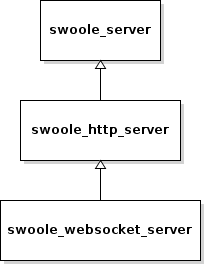
\includegraphics[scale=0.5]{swoole_server.png}
\caption{swoole\_websocket\_server的继承关系}
\end{figure}



下面的示例使用Swoole来实现一个异步非阻塞多进程的WebSocket服务器。

\begin{lstlisting}[language=PHP]
$server = new swoole_websocket_server("0.0.0.0",9501);

$server->on('open',function(swoole_websocket_server $server,$request){
	echo "server: handshake success with fd{$request->fd}\n";
});

$server->on('message',function(swoole_websocket_server $server,$frame){
	echo "receive from {$frame->fd}:{$frame->data}, opcode:{$frame->opcode},fin:{$frame->finish}\n"
	$server->push($frame->fd,"this is server");
});

$server->on('close',function($ser,$fd){
	echo "client {$d} closed\n";
});

$server->start();
\end{lstlisting}

\begin{compactitem}
\item 设置了onRequest回调,websocket服务器也可以同时作为http服务器
\item 未设置onRequest回调,websocket服务器收到http请求后会返回http 400错误页面
\end{compactitem}

\section{onHandShake}

WebSocket建立连接后进行握手,而且WebSocket服务器已经内置了handshake。

如果用户希望自己进行握手处理,可以设置onHandShake事件回调函数。





\begin{lstlisting}[language=PHP]
function onHandShake(swoole_http_request $request, swoole_http_response $response)
\end{lstlisting}

onHandShake事件回调是可选的,而且在设置onHandShake回调函数后不会再触发onOpen事件,需要应用程序代码自行处理。

\section{onOpen}

当WebSocket客户端与服务器建立连接(connect)并完成握手(handshake)后会回调onOpen函数。


\begin{lstlisting}[language=PHP]
function onOpen(swoole_websocket_server $svr,swoole_http_request $req)
\end{lstlisting}

注意,onOpen函数的第2个参数\texttt{swoole\_http\_request \$req}是从1.7.14开始的,之前是\texttt{\$fd}。

\begin{compactitem}
\item \texttt{\$req}是一个Http请求对象,包含了客户端发来的握手请求信息;
\item onOpen事件函数中可以调用push向客户端发送数据或者调用close关闭连接;
\item onOpen事件回调是可选的。
\end{compactitem}

\section{onMessage}

当服务器收到来自客户端的数据帧时会回调onMessage函数。



\begin{lstlisting}[language=PHP]
function onMessage(swoole_server $server, swoole_websocket_frame $frame)
\end{lstlisting}

\begin{compactitem}
\item \texttt{\$frame} 是swoole\_websocket\_frame对象,包含了客户端发来的数据帧信息;
\item onMessage回调必须被设置,不设置onMessage回调则服务器将无法启动。
\end{compactitem}

\subsection{swoole\_websocket\_frame}

swoole\_websocket\_frame共有4个属性,分别是:

\begin{compactitem}
\item \texttt{\$frame->fd},客户端的socket id,使用\texttt{\$server->push}推送数据时需要用到。
\item \texttt{\$frame->data},数据内容,可以是文本内容也可以是二进制数据,可以通过opcode的值来判断。
\item \texttt{\$frame->opcode},WebSocket的OpCode类型,可以参考WebSocket协议标准文档。
\item \texttt{\$frame->finish}, 表示数据帧是否完整,一个WebSocket请求可能会分成多个数据帧进行发送。
\end{compactitem}

如果\texttt{\$data}是文本类型,那么编码格式必然是UTF-8,这是WebSocket协议规定的。

\subsection{OpCode}


\begin{compactitem}
\item \texttt{WEBSOCKET\_OPCODE\_TEXT = 0x1},文本数据
\item \texttt{WEBSOCKET\_OPCODE\_BINARY = 0x2},二进制数据
\end{compactitem}

\section{push}

\texttt{swoole\_websocket\_server->push}用于向websocket客户端连接推送数据,长度最大不得超过2M。


\begin{lstlisting}[language=PHP]
function swoole_websocket_server->push(int $fd, string $data, int $opcode=1,bool $finish=true)
\end{lstlisting}

\begin{compactitem}
\item \texttt{\$fd}是客户端连接的ID,如果指定的\texttt{\$fd}对应的是TCP连接而不是websocket客户端,那么将会发送失败。
\item \texttt{\$data}是要发送的数据内容。

\item \texttt{\$opcode}用于指定发送数据内容的格式,默认为文本。

如果需要发送二进制内容,则需要设置\$opcode参数为WEBSOCKET\_OPCODE\_BINARY\_FRAME。

\item 如果发送成功返回true,发送失败则返回false。

\end{compactitem}


在实际应用中,如果Websocket服务器需要向所有连接的客户端发送广播通知消息,则可以使用foreach循环来实现。


\begin{lstlisting}[language=PHP]
foreach($server->connections as $fd){
	$server->push($fd,json_encode($data));
}
\end{lstlisting}


\subsection{Frame Type}


WebSocket数据帧类型

\begin{compactitem}
\item \texttt{WEBSOCKET\_OPCODE\_TEXT = 0x1},UTF-8文本字符数据
\item \texttt{WEBSOCKET\_OPCODE\_BINARY = 0x2},二进制数据
\end{compactitem}


\subsection{Connection State}

WebSocket连接状态

\begin{compactitem}
\item \texttt{WEBSOCKET\_STATUS\_CONNECTION = 1},连接进入等待握手
\item \texttt{WEBSOCKET\_STATUS\_HANDSHAKE = 2},正在握手
\item \texttt{WEBSOCKET\_STATUS\_FRAME = 3},已握手成功等待浏览器发送数据帧
\end{compactitem}





\begin{lstlisting}[language=PHP]

\end{lstlisting}








\begin{lstlisting}[language=PHP]

\end{lstlisting}




\begin{lstlisting}[language=PHP]

\end{lstlisting}




\begin{lstlisting}[language=PHP]

\end{lstlisting}




\begin{lstlisting}[language=PHP]

\end{lstlisting}



\begin{lstlisting}[language=PHP]

\end{lstlisting}



\begin{lstlisting}[language=PHP]

\end{lstlisting}




\begin{lstlisting}[language=PHP]

\end{lstlisting}




\begin{lstlisting}[language=PHP]

\end{lstlisting}




\begin{lstlisting}[language=PHP]

\end{lstlisting}





\begin{lstlisting}[language=PHP]

\end{lstlisting}



\begin{lstlisting}[language=PHP]

\end{lstlisting}



\begin{lstlisting}[language=PHP]

\end{lstlisting}




\begin{lstlisting}[language=PHP]

\end{lstlisting}




\begin{lstlisting}[language=PHP]

\end{lstlisting}




\begin{lstlisting}[language=PHP]

\end{lstlisting}




\begin{lstlisting}[language=PHP]

\end{lstlisting}



\begin{lstlisting}[language=PHP]

\end{lstlisting}



\begin{lstlisting}[language=PHP]

\end{lstlisting}




\begin{lstlisting}[language=PHP]

\end{lstlisting}




\begin{lstlisting}[language=PHP]

\end{lstlisting}




\begin{lstlisting}[language=PHP]

\end{lstlisting}





\begin{lstlisting}[language=PHP]

\end{lstlisting}



\begin{lstlisting}[language=PHP]

\end{lstlisting}



\begin{lstlisting}[language=PHP]

\end{lstlisting}




\begin{lstlisting}[language=PHP]

\end{lstlisting}




\begin{lstlisting}[language=PHP]

\end{lstlisting}




\begin{lstlisting}[language=PHP]

\end{lstlisting}





\begin{lstlisting}[language=PHP]

\end{lstlisting}



\begin{lstlisting}[language=PHP]

\end{lstlisting}



\begin{lstlisting}[language=PHP]

\end{lstlisting}




\begin{lstlisting}[language=PHP]

\end{lstlisting}




\begin{lstlisting}[language=PHP]

\end{lstlisting}




\begin{lstlisting}[language=PHP]

\end{lstlisting}




\begin{lstlisting}[language=PHP]

\end{lstlisting}



\begin{lstlisting}[language=PHP]

\end{lstlisting}



\begin{lstlisting}[language=PHP]

\end{lstlisting}




\begin{lstlisting}[language=PHP]

\end{lstlisting}




\begin{lstlisting}[language=PHP]

\end{lstlisting}




\begin{lstlisting}[language=PHP]

\end{lstlisting}




\begin{lstlisting}[language=PHP]

\end{lstlisting}



\begin{lstlisting}[language=PHP]

\end{lstlisting}



\begin{lstlisting}[language=PHP]

\end{lstlisting}




\begin{lstlisting}[language=PHP]

\end{lstlisting}




\begin{lstlisting}[language=PHP]

\end{lstlisting}




\begin{lstlisting}[language=PHP]

\end{lstlisting}





\begin{lstlisting}[language=PHP]

\end{lstlisting}



\begin{lstlisting}[language=PHP]

\end{lstlisting}



\begin{lstlisting}[language=PHP]

\end{lstlisting}




\begin{lstlisting}[language=PHP]

\end{lstlisting}




\begin{lstlisting}[language=PHP]

\end{lstlisting}




\begin{lstlisting}[language=PHP]

\end{lstlisting}






\begin{lstlisting}[language=PHP]

\end{lstlisting}



\begin{lstlisting}[language=PHP]

\end{lstlisting}



\begin{lstlisting}[language=PHP]

\end{lstlisting}




\begin{lstlisting}[language=PHP]

\end{lstlisting}




\begin{lstlisting}[language=PHP]

\end{lstlisting}




\begin{lstlisting}[language=PHP]

\end{lstlisting}






\begin{lstlisting}[language=PHP]

\end{lstlisting}



\begin{lstlisting}[language=PHP]

\end{lstlisting}



\begin{lstlisting}[language=PHP]

\end{lstlisting}




\begin{lstlisting}[language=PHP]

\end{lstlisting}




\begin{lstlisting}[language=PHP]

\end{lstlisting}




\begin{lstlisting}[language=PHP]

\end{lstlisting}
%
%
%
\part{Framework}


\chapter{Overview}


与其他Web框架不同,SwooleFramework是一个全功能的后端服务器框架。除了Web方面的应用之外,更广泛的后端程序中都可以使用。


\begin{compactitem}
\item 内置PHP应用服务器,可脱离nginx/php-fpm/apache独立运行
\item 配置化与资源自动工厂,可实现从配置中创建资源对象,完全无需new对象
\item 全面采用命名空间+autoload,代码中无需任何的include/require
\item 全局注册树,所有资源都挂载到全局树上,彻底实现资源的单例管理和懒加载
\item 全栈框架,提供了数据库操作,模板,Cache,日志,队列,上传管理,用户管理等几乎所有的功能
\end{compactitem}

使用内置应用服务器,可节省每次请求代码来的额外消耗,需要安装swoole扩展才能使用SwooleFramework应用服务器。

\begin{compactenum}
\item 使用PECL或手动编译安装Swoole扩展

\begin{lstlisting}[language=bash]
$ sudo pecl install swoole
\end{lstlisting}

\item 修改php.ini加入extension=swoole.so
\end{compactenum}

连接池技术可以很好的帮助存储系统节省连接资源。

Swoole应用服务器支持的特性如下:

\begin{compactitem}
\item 热部署,代码更新后即刻生效,依赖runkit扩展实现。
\item MaxRequest进程回收机制,防止内存泄露
\item 支持使用Windows作为开发环境
\item http KeepAlive,可节省tcp connect带来的开销
\item 静态文件缓存,节省流量
\item 支持Gzip压缩,节省流量
\item 支持MySQL重新连接
\item 支持文件上传
\item 支持POST大文本
\item 支持Session/Cookie
\item 支持Http/FastCGI两种协议
\end{compactitem}

Swoole框架额外提供的网络协议包括WebSocket、HTTP、SOA、SMTP、FTP和异步HTTPClient。

\begin{compactitem}
\item WebSocket协议支持,并附带一个基于websocket协议的webim系统
\item 普通Web服务器,可支持静态文件和普通include php方式的程序
\item SOA逻辑层服务器/客户端,支持并行请求
\item 一个简单的SMTP服务器
\item FtpServer
\item 异步HttpClient
\end{compactitem}



\begin{lstlisting}[language=bash]
<?php
require __DIR__.'/libs/lib_config.php';

$AppSvr = new Swoole\Protocol\AppServer();
$AppSvr->loadSetting(__DIR__."/swoole.ini"); // 加载配置文件
$AppSvr->setAppPath(__DIR__.'/apps/'); // 设置应用所在的目录
$AppSvr->setLogger(new Swoole\Log\EchoLog(false)); // Logger

/**
  * 如果没有安装swoole扩展,这里还可选择
  * 1. BlockTCP 阻塞的TCP,支持windows平台,需要将worker_num设为1
  * 2. SelectTCP 使用select做事件循环,支持windows平台,需要将worker_num设为1
  * 3. EventTCP 使用libevent,需要安装libevent扩展
  */
$server = new \Swoole\Network\Server('0.0.0.0',9501);
$server->setProtocol($AppSvr);
$server->daemonize($AppSvr);
$server->run(array('work_num'=>1,'max_request'=>5000));
\end{lstlisting}

在浏览器中打开\url{http://127.0.0.1:9501/}访问并测试Swoole应用程序。

\begin{lstlisting}[language=bash]
$ sudo php server.php
[2013-07-09 12:17:05]  Swoole. running. on 0.0.0.0:9501
\end{lstlisting}


下面的测试是使用swoole扩展作为底层Server框架的,其他驱动暂未测试。



\begin{lstlisting}
ab -c 100 -n 100000 http://127.0.0.1:9501/hello/index/
This is ApacheBench, Version 2.3 <$Revision: 655654 $>
Copyright 1996 Adam Twiss, Zeus Technology Ltd, http://www.zeustech.net/
Licensed to The Apache Software Foundation, http://www.apache.org/

Benchmarking 127.0.0.1 (be patient)
Completed 10000 requests
Completed 20000 requests
Completed 30000 requests
Completed 40000 requests
Completed 50000 requests
Completed 60000 requests
Completed 70000 requests
Completed 80000 requests
Completed 90000 requests
Completed 100000 requests
Finished 100000 requests


Server Software:        Swoole
Server Hostname:        127.0.0.1
Server Port:            9501

Document Path:          /hello/index/
Document Length:        11 bytes

Concurrency Level:      100
Time taken for tests:   10.717 seconds
Complete requests:      100000
Failed requests:        0
Write errors:           0
Total transferred:      27500000 bytes
HTML transferred:       1100000 bytes
Requests per second:    9330.83 [#/sec] (mean)
Time per request:       10.717 [ms] (mean)
Time per request:       0.107 [ms] (mean, across all concurrent requests)
Transfer rate:          2505.84 [Kbytes/sec] received

Connection Times (ms)
              min  mean[+/-sd] median   max
Connect:        0    1   1.0      1       9
Processing:     1   10   5.6      8      63
Waiting:        0    7   5.4      6      62
Total:          1   11   5.5      9      63

Percentage of the requests served within a certain time (ms)
  50%      9
  66%     11
  75%     12
  80%     13
  90%     17
  95%     22
  98%     28
  99%     32
 100%     63 (longest request)
\end{lstlisting}





\section{URLRewrite}


\subsection{Nginx+FPM+Swoole}



\begin{lstlisting}[language=bash]
server {
  listen 80;
  server_name www.swoole.com;
  root /data/wwwroot/www.swoole.com;
  
  location / {
    if(!-e $request_filename){
       proxy_pass http://127.0.0.1:9501;
    }
  }
}
\end{lstlisting}


\subsection{Apache+Swoole}



\begin{lstlisting}[language=bash]
<VirtualHost *:80>
    ServerName www.swoole.com
    DocumentRoot /data/webroot/www.swoole.com
    DirectoryIndex index.html index.php

    <Directory "/data/webroot/www.swoole.com">
        Options Indexes FollowSymLinks
            AllowOverride None
            Require all granted
    </Directory>

#   ProxyPass /admin !
#   ProxyPass /index.html !
#   ProxyPass /static !
#   ProxyPass / http://127.0.0.1:9501/

    <IfModule mod_rewrite.c>
        RewriteEngine On
        RewriteCond %{DOCUMENT_ROOT}/%{REQUEST_FILENAME} !-f
        RewriteCond %{DOCUMENT_ROOT}/%{REQUEST_FILENAME} !-d
        RewriteRule ^(.*)$ http://127.0.0.1:9501$1 [L,P]
    </IfModule>
</VirtualHost>
\end{lstlisting}










\begin{lstlisting}[language=bash]

\end{lstlisting}






\begin{lstlisting}[language=bash]

\end{lstlisting}






\begin{lstlisting}[language=bash]

\end{lstlisting}





\begin{lstlisting}[language=bash]

\end{lstlisting}





\begin{lstlisting}[language=bash]

\end{lstlisting}





\begin{lstlisting}[language=bash]

\end{lstlisting}





\begin{lstlisting}[language=bash]

\end{lstlisting}






\begin{lstlisting}[language=bash]

\end{lstlisting}






\begin{lstlisting}[language=bash]

\end{lstlisting}





\begin{lstlisting}[language=bash]

\end{lstlisting}





\begin{lstlisting}[language=bash]

\end{lstlisting}





\begin{lstlisting}[language=bash]

\end{lstlisting}





\begin{lstlisting}[language=bash]

\end{lstlisting}






\begin{lstlisting}[language=bash]

\end{lstlisting}






\begin{lstlisting}[language=bash]

\end{lstlisting}





\begin{lstlisting}[language=bash]

\end{lstlisting}





\begin{lstlisting}[language=bash]

\end{lstlisting}





\begin{lstlisting}[language=bash]

\end{lstlisting}





\begin{lstlisting}[language=bash]

\end{lstlisting}






\begin{lstlisting}[language=bash]

\end{lstlisting}

%
%
%
\part{Changelog}


\chapter{Overview}


\begin{compactitem}
\item event-driven
\item asynchronous non-blocking
\item multi-thread reactor
\item multi-process worker
\item multi-protocol
\item millisecond timer
\item async mysql client
\item built-in http/websocket/http2 server
\item async http/websocket client
\item async redis client
\item async task
\item async read/write file system
\item async dns lookup
\item support IPv4/IPv6/UnixSocket/TCP/UDP
\item support SSL/TLS encrypted transmission
\end{compactitem}

swoole从1.5版本开始建立起严格的版本更新记录。平均迭代时间为每半年一个大版本,每2-4周一个小版本。

\begin{compactitem}
\item alpha 特性预览版本,表示开发计划中的任务已完成,进行开放预览,可能会存在较多BUG
\item beta 测试版本,表示已经可以用于开发环境测试,可能存在BUG
\item rc[1-n] 候选发布版本,表示进入发布周期,正在做大范围的测试,在此期间仍可能发现BUG
\item stable 稳定版,表示此版本已完毕,可正式投入使用
\end{compactitem}

单双数版本的意义如下:

\begin{compactitem}
\item 单数版本为特性新增版本,主要工作是新增功能特性、代码重构、结构调整。可能会带来一些BUG。
\item 双数版本为问题修复版本,主要工作是修复现有的已知问题、提升性能、完善细节。稳定性更高
\end{compactitem}



\section{1.5.7}


\begin{compactitem}
\item 不再使用clock\_gettime,不需要如此高精度的时间
\item 增加onWorkerStart/onWorkerStop回调函数
\item 增加onMasterConnect/onMasterClose回调函数
\item 可配置poll线程与worker进程间的通信方式
\end{compactitem}


\section{1.5.8}

\begin{compactitem}
\item 增加swoole\_connection\_list接口,用于遍历所有连接
\item 增加swoole\_connection\_info接口,用于获取连接信息
\item swoole\_server\_send/swoole\_server\_close不再需要传入from\_id参数
\item buffer功能测试通过,已增加到setting中
\item 提供对tcp\_keepalive的支持
\item 增加日志模块,记录运行时的警告和错误信息
\end{compactitem}

\section{1.5.9}


\begin{compactitem}
\item 修复onClose回调\$fd/\$from\_id错误的bug
\item swoole\_framework框架提供WebSocket支持
\end{compactitem}

\section{1.6.0}

\begin{compactitem}
\item 优化UDP实现方式,实现高并发高可靠的UDP Server
\item 可以切换IPC模式,队列或者Unsock
\item close事件处理优化,解决丢失close的bug
\item 使用全局内存池来分配内存
\end{compactitem}


\section{1.6.1}

\begin{compactitem}
\item 增加configure可选参数\texttt{-\/-enable-msgqueue},启用此参数后将使用消息队列作为IPC方式
\item 解决reload后,worker分配错误的bug
\item 抢占式分配bug解决
\item 解决刷warn的问题
\end{compactitem}


\section{1.6.2}


\begin{compactitem}
\item 增加swoole\_event\_add函数,可以将任意一个socket添加到swoole的主事件循环内
\item 增加swoole\_event\_del函数,删除添加的socket
\item 增加examples/proxy.php实例代码,全异步非阻塞的代理服务器
\item 增加examples/async\_mysql.php,实现异步非阻塞的MySQL调用
\end{compactitem}

1.6.2新增的reactor操作接口,使得redis、mysql、mongodb等网络接口整合swoole\_server中,实现全异步化高性能服务器


\section{1.6.3}

\begin{compactitem}
\item SWOOLE\_MODE\_BASE模式重构,由于PHP在多线程下容易发生内存错误,BASE模式修改为单进程单线程模式
\item swoole\_client->on/swoole\_event\_add可以用于任何环境
\item swoole\_server增加面向对象风格
\item swoole\_connection\_info可用于UDP协议
\item 解决php,gcc低版本可能出现的段错误问题
\item 解决swoole扩展导致fpm段错误的问题
\end{compactitem}


\section{1.6.4}


\begin{compactitem}
\item 内存池修改为自动扩容
\item AsyncTask接口
\item 低版本系统bug解决
\item 提供swoole\_lock锁
\end{compactitem}

\section{1.6.5}


\begin{compactitem}
\item 启动100个worker进程时可能crash的问题解决
\item 支持MacOS
\item 定时器重构,支持1ms粒度,并可用于Worker进程
\end{compactitem}


\section{1.6.6}



\begin{compactitem}
\item 对FreeBSD/MacOS下的kqueue做了优化
\item 默认使用epoll/kqueue作为事件轮询
\item swoole\_client内存泄露问题解决
\item 对主动发起close做优化,无需主进程再次发送通知
\item task\_worker使用UnixSock-UDP通信方式
\item 对Epoll的RST事件优化
\end{compactitem}

\section{1.6.7}

\begin{compactitem}
\item 线程的数量加入限制最大不超过CPU数的4倍
\item 进程数量超过CPU数的100倍后会抛一一条警告信息
\item 修复onStart不能addtimer的bug
\item 修复php5.5下异步mysql编译失败问题
\item poll\_thread\_num改为reactor_num
\end{compactitem}

\section{1.6.8}


\begin{compactitem}
\item 解决某些系统下worker进程段错误问题
\item 增加swoole\_server\_taskwait函数
\item 解决UDP多进程在FDMOD模式下的错误问题
\end{compactitem}

\section{1.6.9}

\begin{compactitem}
\item 增加到pecl.php.net,可通过pecl install swoole来安装
\item 修复task模块的bug
\item 增加基于unixsock的争抢模式实现
\end{compactitem}

\section{1.6.10}


\begin{compactitem}
\item 简化异步客户端,当onReceive时不再需要调用\$cli->recv,直接拿到数据。当onClose发生时也不需要再次调用\$cli->close
connect支持填写域名,swoole会自动进行DNS查询
\item 当connect失败时,如果直接仍然调用send/recv,会抛出错误
\item connection信息中增加connect\_time和last\_time,记录连接的时间和最后一次发送数据的时间
\item 增加TCP长连接心跳机制支持
\item 重构data\_buffer功能
\end{compactitem}

\section{1.6.11}


\begin{compactitem}
\item task\_worker启动时也会调用onWorkerStart,可以用worker\_id参数来区分task\_worker还是普通的worker
\item 增加onWorkerError回调,用来捕获worker进程异常退出
\item 使用 \$server->setting属性可以得到运行时配置数组
\item swoole\_server::task和taskwait可以指定发送给哪个task\_worker进程
\item 添加对字节流协议的分包支持,参见 examples/length\_check\_server.php \& length\_check\_client.php
\item 增加 package\_eof 参数,等同于 data\_eof
\end{compactitem}


\section{1.6.13}


\begin{compactitem}
\item 修复异常连接导致服务器死循环的BUG
\item 修复swReactorEpoll\_del抛出WARN的BUG
\end{compactitem}



\section{1.7.0 \& 1.6.12}



\begin{compactitem}
\item reactor线程与writer线程合并
\item 对send优化,加入out\_buffer机制
\item 增加AIO异步读写文件的API
\item 增加DNS异步查询函数
\item swoole\_client在php-fpm或apache mod\_php下支持长连接
\item 增加非Server模式下的异步定时器支持
\item 定时器优化
\item 修复bug
\item 增加sendfile支持
\item onReceive的data变量使用引用方式,减少一次内存复制
\item 消息队列模式增加定时器的支持
\item 增加signalfd的支持,使信号事件也加入到Reactor
\end{compactitem}

\section{1.7.1}

\begin{compactitem}
\item 增加unix sock监听的支持
\item 增加swoole\_event\_set函数
\item client对out\_buffer的支持
\item 修复swoole\_server->send后close发生错误的问题
\item 可动态配置IPC方式, 选择消息队列/UnixSock管道
\end{compactitem}

\section{1.7.2}

\begin{compactitem}
\item 增加swoole\_process模块
\item 支持标准输入输出重定向
\item 修复MacOS/FreeBSD/低版本Linux下时钟无法使用的BUG
\item Task进程可以单独配置为使用消息队列通信
\item 修复心跳检测未关闭socket的BUG
\end{compactitem}

\section{1.7.3}


\begin{compactitem}
\item 增加swoole\_process->exec接口
\item 修复连接后立即关闭的BUG
\item 优化swoole\_server->send发送大包
\item 修复dispatch\_mode = 3不生效问题
\item 修复length\_check错误问题
\end{compactitem}

\section{1.7.4}

\begin{compactitem}
\item reload对task\_worker有效
\item 当管道写满是进行poll等待可写,而不是丢包
\item 增加对clang编译器的支持
\item 修复shutdown过程task\_worker/manager非正常结束问题
\item Task进程支持定时器
\item 修复UDP发送错误的BUG
\item 增加SSL-server的支持
\end{compactitem}

\section{1.7.5}


\begin{compactitem}
\item 增加swoole\_table
\item 增加swoole\_client->sendfile()
\item 增加swoole\_server->stats()函数,用于统计服务器网络请求数
\item 增加worker和master之间unix的内存缓存
\item 增加swoole\_process支持使用消息队列做进程间通信
\item 增加swoole\_client构造函数增加第3个参数,作为长连接的ID
\item 增加swoole\_process::daemon函数
\item 增加Append写的支持,swoole\_async\_write的offset为-1表示追加到文件末尾
\item 增加swoole\_server->gettimer()获取所有定时器设置
\item 增加task进程单独设置max\_requset/ipc\_mode的支持
\item 优化worker和master之间的通信
\item 优化TCP短链接,性能提升50\%
\item 修复connection\_info在UDP客户端下端口号错误问题
\item 修复swoole\_server->master\_pid某些情况下不可用问题
\item 修复定时器第一次设置超过当前时间2倍的BUG
\item 修复异步任务结束后进程无法自动退出问题
\item 修复swoole\_event\_add重复添加相同fd时出错的问题
\item 修复swoole\_process->\$pid不可用的问题,在任何环境下均可获取到正确的pid
\item 移除onMasterClose/onMasterConnect
\end{compactitem}

\section{1.7.6}

1.7.6是针对1.7.5的BUG修复版。

\begin{compactitem}
\item 增加php.ini中可配置aio\_thread\_num,AIO的线程数量
\item 增加Manager进程退出的监控
\item 修复onConnect/onClose无法正确投递到对应worker的BUG
\item 修复消息队列模式发生死循环的BUG
\item 修复swoole\_table->set发生死循环问题
\item 修复enable-ringbuffer后执行错误的问题
\item 移除enable-msgqueue编译参数
\item 修复定时器第一次触发时间错误的BUG
\item sendfile增加nopush的设置
\end{compactitem}


\section{1.7.7}

\begin{compactitem}
\item 增加对cygwin环境的支持,仅支持SWOOLE\_BASE模式
\item 修复swoole\_process子进程接收不到信号的问题
\item 定时器重构,使用EventLoop的超时机制来实现定时器
\item 定时器增加after接口,一次性时间回调
\item onClose事件调整为在close前触发
\item 支持在swoole\_server的worker进程中创建swoole_process子进程
\item 默认package\_max\_length为2M
\item 支持用户设置task临时文件目录
\end{compactitem}

\section{1.7.8}


\begin{compactitem}
\item 修复swoole\_http\_server::on未执行父类方法的问题
\item 修复swoole\_http\_server中COOKIE无法读取的问题
\item 增加swoole\_http\_server对POST RawContent的支持
\item after接口可以传入一个用户参数
\item swoole\_client->recv和onReceive的data变量修改为零拷贝
\item swoole\_client->onReceive改为ET模式
\item 修复swoole\_table->set无法设置超过64K字符串的问题
\item 重构swoole\_table,解决foreach可能存在的数据同步问题
\item 增加在php.ini中的配置项swoole.display\_errors,用于关闭错误信息
\item swoole\_timer\_after/swoole\_server->after接口增加一个可选参数,可以将一个自定义变量传递到回调函数中
\item 修复open\_length\_check连接内存缓冲区未重置的BUG
\item 增加dispatch\_mode=4,按照客户端IP取摸分配worker进程
\item 事件回调函数中捕获到异常错误等级由E\_WARNING调整为E\_ERROR
\end{compactitem}

\section{1.7.9}


\begin{compactitem}
\item 增加内置WebSocket协议支持
\item swoole\_process在构造之后就可以访问到pipe的值
\item 增加swoole\_process::signal/swoole\_async\_signal用于异步信号
\item 增加swoole\_server->addProcess,可以添加用户定义的子进程到Server
\item 增加swoole\_process::name方法
\item 增加swoole\_server::listen方法
\item 增加swoole\_server::sendMessage和onPipeMessage用于操作底层管道通信
\item 增加swoole\_event\_write函数
\item 增加swoole\_process->close方法
\item 增加user/group配置项,可以修改Worker进程的用户和组
\item swoole\_server的task/finish方法可以直接发送任意PHP变量,扩展内对非字符类型自行串化/反串化
\end{compactitem}

\section{1.7.10}



\begin{compactitem}
\item 修复UDP在reload之后发生死循环的BUG
\item 修复Http服务器POST发生段错误的问题
\item 增加swoole\_http\_server->push方法,用于向WebSocket客户端推送消息
\item 增加Http请求头信息到swoole\_http\_server合并全局变量\$\_SERVER中
\item 增加swoole\_process::wait的非阻塞设置
\item 修复合并全局变量未替换中横线为下划线的BUG
\item 修复swoole\_http\_request的key变为大写的BUG
\item 修复pecl脚本无法直接安装的问题
\item 修复swoole\_server->addProcess在未使用管道时发送段错误的问题
\item 修复swoole\_server->sendMessage失败的问题
\item 修复swoole\_process子进程无法打开标准输入的问题
\item 增加swoole\_server->sendto方法,用于向任意IP:PORT发送UDP包
\item 优化swoole\_client/swoole\_event性能,减少hashtable查找
\item 优化swoole\_http\_server性能
\item 修复ARM平台编译错误的问题,1.7.10版本可用于ARM平台
\item 修复task\_tmpdir设置导致投递任务失败的问题
\end{compactitem}


\section{1.7.11}

\begin{compactitem}
\item 修复UDP服务器调用connection\_info发生错误的问题
\item 修复task临时文件磁盘空间未释放的BUG
\item 修复WebSocket服务器onOpen事件回调中执行close导致进程崩溃的问题
\item 修复在task进程中调用sendMessage导致进程崩溃的问题
\item 修复websocket服务器握手时Sec-WebSocket-Accept串偶发错误的问题
\item 修复Http服务器在开启KeepAlive时连续POST数据发生coredump的问题
\item 修复MacOS/FreeBSD在大量并发时出现ENOBUFF错误
\item 增加Http服务器分片(chunk)发送的支持
\item 增加pcre检测,如果未安装pcre库将关闭swoole\_table的foreach遍历接口
\end{compactitem}

\section{1.7.12}


\begin{compactitem}
\item 修复TCP缓存区发生错误的问题
\item 客户端recv方法未启用waitall, buffer\_size最大限制为64K
\item 删除无用的错误日志
\end{compactitem}


\section{1.7.13}


\begin{compactitem}
\item 服务器session\_list尺寸调整为1M
\item connection\_info中的from\_fd, from\_port 修改为 server\_fd, server\_port
\item 服务器只在监听多个端口,connection\_info返回 server\_fd, server\_port
\item connection\_info增加对IPv6 TCP协议的支持
\item connection\_info增加socket\_type项表示客户端的类型
\item 优化Http服务器性能
\item 优化WebSocket服务器性能
\item 修复文件描述符过多后Accept发生死循环的BUG
\item 修复reload期间某个worker进程退出导致管理进程死循环的BUG
\item 增加swoole\_client->getsockname用于获取本地socket的ip和port
\item 增加swoole\_client->getpeername用于获取远程对端socket的ip和port
\item 增加swoole\_client->sendto可向任意UDP服务器发送数据包
\end{compactitem}


\section{1.7.14}


\begin{compactitem}
\item WebSocket服务器onOpen回调函数第2个参数由\$fd调整为\$request对象
\item WebSocket服务器onHandShake回调函数中执行close不回调onOpen
\item PHP5.3不再需要脚本末尾手工加swoole\_event\_wait
\item 增加swoole\_server->tick和swoole\_timer\_tick函数
\item 修复onReceive数据合并失效的BUG
\item Http服务器增加gzip压缩的支持
\item swoole\_server->send支持发送swoole\_buffer对象
\item Http服务器允许发送空body的response
\end{compactitem}



\section{1.7.15}



\begin{compactitem}
\item 修复swoole\_client的waitall参数失效问题
\item 修复swoole\_table发生死循环的BUG
\item 禁用swoole\_websocket\_server->send方法
\item 增加swoole\_table->incr/decr原子自增/自减方法
\item BASE模式支持向任意FD发送数据
\item 修复Accept失败返回Too Many Connection重复打印日志的问题
\item 设置dispatch\_mode = 1, 3 后关闭onClose/onConnect事件回调
\item 修复低版本Linux下Accept未设置阻塞的问题
\item 允许Worker进程内设置非系统保留信号
\item 增加open\_eof\_split配置,使用EOF检测可以支持自动分包
\end{compactitem}


\section{1.7.16}


\begin{compactitem}
\item 修复swoole\_server->addtimer与tick定时器冲突的BUG
\item 增加server统计项request\_count和worker\_request\_count
\item 移除swoole底层对对象资源属性的依赖,直接读取指针,提升性能
\item 解决心跳线程无法强制杀掉遗留连接的问题
\item 增加server的连接迭代器,可以使用foreach遍历服务器的所有连接
\item 增加客户端自动协议处理的支持,可以使用open\_eof\_split/open\_length\_check配置
\item 增加SWOOLE\_PACKET标志位用于支持TCP透传模式
\item 优化dispatch\_mode=3模式,提升任务分配的效率
\item 增加http服务器multipart-form和上传文件的支持
\item 修复task\_max\_request参数失效的问题
\item 增加http服务器请求的query\_string
\end{compactitem}



\section{1.7.17}


\begin{compactitem}
\item 使用pthread\_barrier\_wait代替sleep加快程序启动速度
\item 修复swoole\_client异步模式下send数据不完整的BUG
\item 移除task\_dispatch\_mode配置项
\item 默认task进程的max\_request改为0,不自动退出进程
\item Http服务器上传文件使用mktemp系统调用
\item 修复EOF\_check特性导致主进程coredump的问题
\item 增加pipe\_buffer\_size配置项,用于调整管道通信的缓存区尺寸
\item 管道内存缓存区默认尺寸调整为32M
\item Http服务器Header最大长度由128调整为8192
\item 修复swoole\_process->pop发生错误的问题
\item 修复taskwait接口在MacOS/CygWin环境下超时的问题
\item 增加swoole\_table->exist方法
\end{compactitem}



\section{1.7.18}


\begin{compactitem}
\item 增加onPacket事件回调函数,使UDP包与TCP分离
\item 修复EOF协议处理时发生错误的问题
\item 兼容PHP7版本
\item 修复swoole\_http\_response->header导致内存泄漏的问题
\item 长度检测协议允许0长度无包体的请求
\item swoole\_table支持有符号整数
\item 支持REUSEPORT特性,短连接TCP服务性能提升200\%(仅支持Linux 3.9.0或更高版本)
\item 修复swoole\_client/swoole\_timer内存泄漏问题
\item 增加enable\_unsafe\_event配置,允许在dispatch\_mode=1/3时开启Connect/Close事件
\item 增加swoole\_process::setaffinity方法用于设置CPU亲和性
\item swoole\_client->set增加socket\_buffer\_size配置
\item 增加swoole\_server->exist方法,用于检测\$fd对应的TCP客户端连接是否存在
\item 函数风格的API即将移除
\item swoole\_server->handler方法即将移除
\item addtimer/deltimer/swoole\_timer\_add/swoole\_timer\_del接口即将移除,请使用tick/after定时器
\end{compactitem}


\section{1.7.19}



\begin{compactitem}
\item 增加swoole\_atomic模块,支持原子整数操作
\item 修复定时器在系统休眠后无法恢复运行的BUG
\item 修复SSL服务器在慢速网络中发送超过30K大包失败的问题
\item UDP/UDP6/UNIX\_DGRAM协议支持64K大包
\item 修复addtimer/tick定时器在BASE模式下无法使用的问题
\item 修复swoole\_process子进程退出时消息队列被自动销毁的问题
\item 增加SWOOLE\_BASE模式下对addProcess的支持
\item 修复SWOOLE\_KEEP发生段错误的问题
\end{compactitem}



\section{1.7.20}



\begin{compactitem}
\item swoole\_http\_request->rawContent() 函数在任意情况下都可以取到POST Body
\item 修复swoole\_process::useQueue()第一个参数为0时消息队列泄漏的问题
\item 增加swoole\_http\_server的DELETE包体支持,可以在\$req->post中得到请求参数
\item 增加swoole\_client对SSL/TLS隧道加密的支持
\item 优化RINIT/RSHUTDOWN代码,减少扩展在php-fpm环境下的性能消耗
\item 优化SSL的onConnect事件顺序,在SSL握手完成后回调onConnect函数
\item 增加swoole\_server/swoole\_client的SSL方法配置
\item 修复swoole\_websocket\_server未设置onRequest时coredump的问题
\item 增加swoole\_server->getClientInfo/getClientList别名
\item 修复swoole\_server->finish在BASE模式下不可用的问题
\item 禁止在onStart回调函数中调用swoole\_server->task/taskwait
\item 增加swoole\_client设置SSL证书的支持
\item 修复swoole\_http\_server内存泄漏的问题
\end{compactitem}


\section{1.7.21}

\begin{compactitem}
\item 修复swoole\_client同步模式在服务器主动关闭时发生内存泄漏的问题
\item 修复POST/文件上传超过8K无法处理的问题
\item 增加swoole\_http\_response->sendfile方法,用于发送大文件
\item 修复swoole\_client启用SSL/TLS隧道加密后close发生coredump的问题
\item 增加swoole\_server->getSocket/swoole\_client->getSocket将Socket导出为sockets扩展资源
\item 增加UDP多播(udp multicast)示例
\item 修复MIPS平台编译错误的问题
\item 修复UDP大包在dispatch\_mode=1/3时Worker进程发生死锁的问题
\item 增加swoole\_client->sleep/wakeup方法,用于暂停/恢复数据接收事件
\item 修复UDP大包中间数据异常问题(重要BUG)
\end{compactitem}


\section{1.7.22}


\begin{compactitem}
\item 修复PHP7下HttpServer发生内存泄漏的问题
\item 修复PHP7下core dump的问题
\item 修复swoole\_table->del出现错误的问题(重要问题)
\item 增加swoole\_client->send/recv的socket参数选项
\item 增加swoole\_async\_set新配置socket\_dontwait/socket\_buffer\_size/enable\_signalfd
\item 增加SSL/TLS客户端证书验证支持
\item 修复tick定时器长时间运行整形溢出导致停止运行的问题
\item 增加swoole\_websocket\_server->exist用于判断一个fd是否为正确的连接
\item 增加原生MySQL异步客户端
\end{compactitem}


\section{1.8.0}


\subsection{客户端}


\begin{compactitem}
\item 增加原生异步MySQL客户端
\item 增加原生异步Redis客户端,基于Redis官方提供的hiredis库
\item 增加原生异步Http客户端
\item 增加原生异步WebSocket客户端支持
\item 重构底层swClient,异步TCP客户端实现放到swoole内核中
\item 增加swoole\_client->reuse属性,SWOOLE\_KEEP长连接模式下标识是否为复用的连接
\end{compactitem}

\subsection{服务器端}


\begin{compactitem}
\item 重构websocket服务器代码,底层与length\_check协议复用相同的处理函数,增强稳定性
\item 增加Task进程对tick/after定时器的支持,底层基于高精度的setitimer+信号实现
\item 保存构造函数中传入的host、port参数到swoole\_server对象属性
\item 增加多端口多协议的支持(重要更新)
\item 增加swoole\_server->defer函数用于延时执行一些函数
\item 增加swoole\_server->close强制切断连接的选项,设置第二个参数会true会清空发送队列并立即切断连接
\end{compactitem}

\begin{example}
多端口多协议示例
\begin{lstlisting}[language=PHP]
<?php
$serv = new swoole_server("0.0.0.1",9501);

$port2 = $serv->listen("127.0.0.1",9502,SWOOLE_SOCK_TCP);\

$port2->set(array(
       'open_length_check'=>true,
       'package_length_type'=>'N',
       'package_length_offset'=>0,
       'package_body_offset'=>4,
       'package_max_length'=>2000000,//协议最大长度
   )
);

$port2->on('receive',function(swoole_server $serv, $fd, $from_id, $data){
   echo "ServerPort2\n";
});

$serv->on('connect',function($serv,$fd,$from_id){
   echo "[#" . posix_getpid() . "]\tClient@[$fd:$from_id]: Connect.\n";
});

$serv->on('receive',function(swoole_server $serv, $fd,$from_id,$data){
   echo "[#" . $serv->worker_id . "]\tClient[$fd]: $data\n";
   if($serv->send($fd,"hello\n")==false){
      echo "error\n";
   }
});

$serv->on('close',function($serv,$fd,$from_id){
   echo "[#" . posix_getpid() . "]\tClient@[$fd:$from_id]: Close.\n";
});
\end{lstlisting}
\end{example}

swoole\_table保存Key值会增加内存占用,如table的size为100万,KEY值存储会增加64M内存占用

\begin{compactitem}
\item 增加swoole\_table对key值的存储,foreach遍历table时可以获取到key值
\item 更改swoole\_table的key对比模式,从crc32比对改为直接进行字符串对比
\item 更新utlist.h库到1.9.9版本
\item 修复启用消息队列后发生double-free问题
\item 重构定时器,修复after、tick定时器偶然出现的core dump的问题
\item 定时器使用最小堆数据结构,插入/删除时间复杂度为log(N)
\item 修复swoole\_process::signal在PHP7下发生core dump的问题
\item 修复swoole\_async\_write在PHP7下发生core dump的问题
\item 移除未支持的特性相关历史遗留代码,如heartbeat\_ping、dispatch\_key\_type等
\item 移除swoole\_server->addtimer、swoole\_server->deltimer、swoole\_server->gettimer
\item 移除swoole\_timer\_add、swoole\_timer\_del
\item 移除swoole\_server的onTimer事件
\item 移除task\_worker\_max配置及相关特性代码
\item 移除swoole\_server->handler方法
\end{compactitem}


从1.8.0-rc2开始,swoole\_process只支持cli模式。

\section{1.8.1}


\begin{compactitem}
\item 增加核心类的命名空间别名
\item 增加swoole\_server->protect方法,用于保护某些连接不被心跳线程切断
\item 增加swoole\_websocker\_server::pack和swoole\_websocker\_server::unpack静态方法,用于手工打包/解包websocket数据帧
\item 修复日志打印标准输出被关闭不断产生SIGPIPE信号导致死循环的问题
\item 修复MacOS环境下启用openssl编译失败的问题
\item 增加对redis订阅和发布消息的支持
\item 修复多端口监听未设置监听端口回调发生core dump的问题
\item 修复异步Client发生内存泄漏的问题
\item 修复在其他事件回调函数中关闭异步Client偶然发生core dump的问题
\item 增加swoole\_http\_client对gzip内容压缩的支持
\end{compactitem}


使用命名空间类风格,需要修改php.ini,增加swoole.use\_namespace=On开启。使用命名空间类名后,旧式的下划线风格类名将不可用


\begin{lstlisting}[language=PHP]
use Swoole\Http\Server;
use Swoole\Http\Request;
use Swoole\Http\Response;

$serv = new Server('127.0.0.1',9501);

$serv->on('Request',function(Request $req, Response $resp){
    var_dump($req->header,get_class($req));
    $resp->send("<h1>Hello Swoole</h1>");
});

$serv->start();
\end{lstlisting}


\section{1.8.2}


\begin{compactitem}
\item 增加对Http2的支持(重要更新)
\item 修复WebSocket服务器接收超过64K数据发生崩溃的问题
\item 修复多端口监听未设置回调函数导致程序崩溃的问题
\item 提升SSL/TLS隧道加密的安全等级,现在默认使用TLS1.2/ECDHA_RSA加密算法
\item 修复onFinish事件回调内存泄漏的问题
\item 修复BASE模式下task finish无法使用的问题
\item 增加log\_level设置,可以选择错误日志的等级
\end{compactitem}


\section{1.8.3}


\begin{compactitem}
\item 增加swoole\_server->getLastError方法,用于获取最近一次操作的错误码
\item 增加Http2协议下对COOKIE的支持
\item 增加Http2协议下对form-data的支持
\item 修复reactor\_num设置超过CPU核数时发生崩溃的问题
\item 修复Swoole\textbackslash Client->on设置的回调函数发生内存泄漏问题
\item 修复打开文件未关闭并且task\_worker\_num设置过大超过256导致服务器程序崩溃
\item 增加全异步服务器安全reload的支持
\item 增加http客户端对COOKIE的支持
\item 增加http客户端对SSL/TLS加密的支持
\item 修复BASE模式下启用心跳检测检测后使用swoole\_client出现异常的问题
\end{compactitem}

\section{1.8.4}

\begin{compactitem}
\item 同步客户端禁止使用Swoole\textbackslash Client->on注册异步回调函数
\item 修复Swoole\textbackslash Http\textbackslash Server解析form-data格式数据发生错误的问题
\item 修复Swoole\textbackslash Redis回调函数内存泄漏问题
\item 修复swoole\_mysql\_query回调函数内存泄漏问题
\item 修复Swoole\textbackslash Http\textbackslash Client内存泄漏问题
\item 修复Swoole\textbackslash Client连接关闭时发生崩溃的问题
\item 修复Swoole\textbackslash Client->onError时未设置errCode的问题
\item 修复swoole\_async\_writefile函数未设置回调函数发生coredump的问题
\item 增加Swoole\textbackslashClient对异步unixsock的支持
\item 增加Swoole\textbackslash Http\textbackslash Request对高精度请求时间的支持
\end{compactitem}



\section{1.8.5}


\begin{compactitem}
\item 修复swoole\_mysql\_query执行insert语句时insert\_id错误的问题(严重问题)
\item 修复Swoole\textbackslash WebSocket\textbackslash Server接收小于4字节数据时发生崩溃的问题(严重问题)
\item 增加swoole\_mysql\_query对bigint自增ID的支持
\item 增加swoole\_mysql\_query嵌套回调出现致命错误的问题
\item 增加execinfo模块检测避免在不支持execinfo平台无法编译通过的问题
\item 修改Swoole\textbackslash Server回调函数存储方式,使用对象属性保存callback
\item 修复Swoole\textbackslash WebSocket\textbackslash Server多协议下发生崩溃的问题
\item 禁止异步Swoole\textbackslash Client使用SWOOKE\_KEEP长连接设置
\item 修复同步Swoole\textbackslash Client内存泄漏问题
\item 增加Swoole\textbackslash Client绑定地址和端口的支持
\item 增加Swoole\textbackslash Server->stats方法的Task消息队列数量和字节计数
\item 修复Swoole\textbackslash Http\textbackslash Client连接关闭时发生崩溃的问题
\item 修复Swoole\textbackslash Server->taskwait操作导致tasking\_num计数错误问题
\end{compactitem}

\section{1.8.6}


1.8.6版本是一个重要的BUG修复版本,主要修复了PHP7环境下HttpServer、TCPClient、HttpClient、Redis等客户端存在的内存泄漏、崩溃问题。

另外,1.8.6版本对MySQL进行了彻底重构,提供了全新的面向对象风格API,彻底移除了对PHP的mysqli和mysqlnd的依赖。

建议所有swoole开发者升级至此版本。


\begin{compactitem}
\item 修复Swoole\textbackslash Server->set方法在关联索引数组的Value为NULL时错误地更改了zval类型
\item 更新Swoole\textbackslash Server->task方法第三个参数可以直接传入回调函数
\item 修复Swoole\textbackslash WebSocket\textbackslash Server收到恶意请求时崩溃的问题,提升稳定性
\item 重构Swoole\textbackslash MySQL客户端,移除对mysqli和mysqlnd的依赖,提供了面向对象风格的API
\item 调整Swoole\textbackslash Http\textbackslash Client为内置,不需要额外的编译参数开启
\item 调整Swoole\textbackslash Client和Swoole\textbackslash Http\textbackslash Client内存回收的时机,在连接发送关闭时回收内存资源
\item 增加swoole\_async\_dns\_lookup查询结果缓存
\item 优化Swoole\textbackslash WebSocket\textbackslash Server性能,减少两次内存复制
\item 移除Swoole\textbackslash Http\textbackslash Server->setGlobal方法
\item 修复在Task进程中执行close时onClose回调函数未在Worker进程中执行的问题
\item 修复Swoole\textbackslash Table删除KEY后未清空数据的问题
\item 增加SSL、TLS证书链的支持
\item 移除gcc aio
\item 修复异步文件读写函数的相关问题
\end{compactitem}



\begin{example}
异步MySQL客户端
\begin{lstlisting}[language=PHP]
<?php
$db = new swoole_mysql;
$server = array(
   'host'=>'192.168.56.102',
   'user'=>'root',
   'password'=>'test',
   'database'=>'test',
);

$db->connect($server,function($db,$r){
   if($r===false){
      var_dump($db->connect_errno,$db->connect_error);
      die;
   }
   
   $sql='show tables';
   $db->query($sql,function(swoole_mysql $db,$f){
      global $s;
      if($r === false){
         var_dump($db->error,$db->errno);
      }elseif($r === true){
         var_dump($db->affected_rows,$db->insert_id);
      }
      var_dump($r);
      $db->close();
   });
});
\end{lstlisting}
\end{example}



\section{1.8.7}


\begin{compactitem}
\item 修复Swoole\textbackslash Http\textbackslash Server在PHP7下崩溃的问题(zdata请求数据内存释放问题)
\item 修复Swoole\textbackslash Http\textbackslash Client的WebSocket模块未设置Header发生崩溃的问题
\item 修复Swoole\textbackslash MySQL对unixsock服务器端主机地址解析错误的问题
\item 修复Swoole\textbackslash Http\textbackslash Client在低于Linux-2.6.18版本内核发生崩溃的问题
\item 修复Swoole\textbackslash MySQL在PHP7下嵌套回调发生崩溃的问题
\item 更新Swoole\textbackslash Server最大监听端口数,由128调整为60000
\item 更新Swoole\textbackslash Server主线程使用epoll或kqueue
\item 修复swoole\_async\_dns\_lookup命中缓存时发生崩溃的问题
\item 修复Swoole\textbackslash Table迭代器在并发读写时发生数据读取错误的问题
\item 修复Swoole\textbackslash Timer::after接口初始化添加时执行顺序错乱问题
\item 增加Swoole\textbackslash Timer::exists接口用于查询定时器是否存在
\item 修复Swoole\textbackslash WebSocket\textbackslash Server::exist方法用于判断其他TCP端口时总是返回false的问题
\item 优化Swoole\textbackslash Server关闭服务时Task进程的结束速度
\end{compactitem}



\section{1.8.8}


\begin{compactitem}
\item 增加Swoole\textbackslash Server\textbackslash Port->getSocket方法,可获取监听端口的socket句柄
\item 增加\texttt{Swoole\textbackslash Server->getClientInfo()['close\_errno']}属性,可获取连接关闭的错误码
\item 修复Swoole\textbackslash Server->close无法关闭未完成握手的SSL客户端连接的问题
\item 修复Swoole\textbackslash Server->taskwait在BASE模式下无法使用的问题
\item 增加Swoole\textbackslash Event命名空间与类风格的API
\item 修复Swoole\textbackslash MySQL客户端无法支持超过250字段查询语句的问题
\item 增加Swoole\textbackslash MySQL字符集设置支持
\item 修复Swoole\textbackslash Server->task第三参数传入Callback在PHP7下发生崩溃的问题
\item 修复Swoole\textbackslash Http\textbackslash Server由于外部引用request对象后用户取消请求导致崩溃的问题
\item 增加Swoole\textbackslash Server->taskWaitMulti可以并发执行多个任务
\item 修复Swoole\textbackslash Http\textbackslash Client的WebSocket客户端接收数据粘包的问题
\item 增加Swoole\textbackslash Server\textbackslash Port对Request、Open、HandShake、Message回调函数设置支持
\item 增加Swoole\textbackslash Client->getPeerCert方法
\item 增加Swoole\textbackslash Client->pause和Swoole\textbackslash Client->resume
\item 增加Swoole\textbackslash Http\textbackslash Client更多的客户端设置选项
\item 修复Swoole\textbackslash Http\textbackslash Request->files在PHP7下为NULL时被外部引用发生崩溃的问题
\end{compactitem}



之前的版本taskwait只支持同时执行一个任务,在一些场景下需要同时并发执行多个Task,并返回结果集。最新的1.8.8版本增加了并发Task的支持,可以解决此类问题。


\begin{example}
异步MySQL客户端
\begin{lstlisting}[language=PHP]
<?php
$tasks[] = mt_rand(1000,9999);
$tasks[] = mt_rand(1000,9999);
//等待所有Task结果返回,超时为10s
var_dump($tasks);

$result = $serv->taskWaitMulti($tasks,10.0);
var_dump($result);
\end{lstlisting}
\end{example}


\section{1.8.9}


\begin{compactitem}
\item 增加命名空间别名设置,现在命名空间类和非命名空间类可以同时使用
\item 修复Swoole\textbackslash MySQL连接某些版本MySQL服务器发生错误的问题
\item 修复Swoole\textbackslash Http\textbackslash Client在回调函数中关闭连接发生崩溃的问题
\item 增加Swoole\textbackslash Http\textbackslash Client->addFile接口,支持POST文件
\item 修复Swoole\textbackslash Http\textbackslash Server在PHP7环境上传文件时偶然发生崩溃的问题
\item 修复Swoole\textbackslash MySQL在PHP7下内存泄漏问题
\item 修复Swoole\textbackslash Redis在PHP7下内存泄漏问题
\item 修复Swoole\textbackslash Http\textbackslash Client在PHP7下内存泄漏问题
\item 修复Swoole\textbackslash Server启用SSL加密未输入证书密码导致崩溃的问题
\item 增加Swoole\textbackslash Http\textbackslash Client对没有ContentLength的响应体的支持
\item 增加-\/-with-openssl编译选项,可指定openssl库的路径
\end{compactitem}


\section{1.9.1}


\begin{compactitem}
\item 修复使用addProcess添加用户进程后无法正常shutdown的问题
\item 异步读写文件函数Async::writeFile增加FILE\_APPEND选项支持
\item 异步读写文件函数在进行read、write时对文件加锁
\item 修复Async::write函数未设置回调函数发生崩溃的问题
\item 重构Async::write函数追加模式的实现,使用O\_APPEND
\item 重构reopen log file特性,收到SIGRTMIN信号后重新打开日志文件并重定向标准输出
\item 修复Table迭代器遗漏数据的问题
\item 回调函数onPacket客户端信息参数增加服务器来源端口server\_port
\item 回调函数onReceive和connection\_info方法即将移除对UDP的支持,UDP端口使用这2个特性时会抛出E\_DEPRECATED警告信息
\item 服务器连接迭代器Connection\textbackslash Iterator增加ArrayAccess接口
\item 修复Server在进程管道缓存区塞满后连续发送大数据导致死锁的问题(重要问题)
\item 修复PHP7下启用opcache导致崩溃的问题
\item 修复taskWaitMulti在超时后无法返回执行成功任务结果的问题
\item 定时器使用MONOTONIC单调时间,解决系统时间修改导致定时器错乱的问题
\end{compactitem}


连接ArrayAccess用法的用法如下:

\begin{lstlisting}[language=PHP]
<?php
$serv->on('connect',function($serv,$fd,$reactor_id){
    echo "IP Address: ".$serv->connections[$fd]['remote_ip']."\n";
    if(isset($serv->connections[6])){
        echo "connection 6 is exists.\n";
    }
});
\end{lstlisting}



\section{2.0.5}


计划实现如下的支持协程的回调方法:

\begin{compactitem}
\item onConnect
\item onReceive
\item onPacket
\item onRequest
\item onHandShake
\end{compactitem}


\section{2.0.6}

计划实现如下的支持协程的回调方法:

\begin{compactitem}
\item onMessage
\end{compactitem}

\section{2.0.7}

计划实现如下的支持协程的回调方法:

\begin{compactitem}
\item onOpen
\item Redis\textbackslash Server->handler
\end{compactitem}






%
%
%
%\include{report}
%
%
%
%
%\include{app}
%
%
%
%\include{system}
%
%
%
%\include{IM}
%
%\include{controlpanel}
%
%
%
%\include{password}




\end{document}